 % ******************************* PhD Thesis Template **************************
% Please have a look at the README.md file for info on how to use the template

\documentclass[a4paper,12pt,times,numbered,print,index]{Classes/PhDThesisPSnPDF}

% ******************************************************************************
% ******************************* Class Options ********************************
% *********************** See README for more details **************************
% ******************************************************************************

% `a4paper'(The University of Cambridge PhD thesis guidelines recommends a page
% size a4 - default option) or `a5paper': A5 Paper size is also allowed as per
% the Cambridge University Engineering Deparment guidelines for PhD thesis
%
% `11pt' or `12pt'(default): Font Size 10pt is NOT recommended by the University
% guidelines
%
% `oneside' or `twoside'(default): Printing double side (twoside) or single
% side.
%
% `print': Use `print' for print version with appropriate margins and page
% layout. Leaving the options field blank will activate Online version.
%
% `index': For index at the end of the thesis
%
% `draftclassic': For draft mode without loading any images (same as draft in book)
%
% `draft': Special draft mode with line numbers, images, and water mark with
% timestamp and custom text. Position of the text can also be modified.
%
% `abstract': To generate only the title page and abstract page with
% dissertation title and name, to submit to the Student Registry
%
% `chapter`: This option enables only the specified chapter and it's references
%  Useful for review and corrections.
%
% ************************* Custom Page Margins ********************************
%
% `custommargin`: Use `custommargin' in options to activate custom page margins,
% which can be defined in the preamble.tex. Custom margin will override
% print/online margin setup.
%
% *********************** Choosing the Fonts in Class Options ******************
%
% `times' : Times font with math support. (The Cambridge University guidelines
% recommend using times)
%
% `fourier': Utopia Font with Fourier Math font (Font has to be installed)
%            It's a free font.
%
% `customfont': Use `customfont' option in the document class and load the
% package in the preamble.tex
%
% default or leave empty: `Latin Modern' font will be loaded.
%
% ********************** Choosing the Bibliography style ***********************
%
% `authoryear': For author-year citation eg., Krishna (2013)
%
% `numbered': (Default Option) For numbered and sorted citation e.g., [1,5,2]
%
% `custombib': Define your own bibliography style in the `preamble.tex' file.
%              `\RequirePackage[square, sort, numbers, authoryear]{natbib}'.
%              This can be also used to load biblatex instead of natbib
%              (See Preamble)
%
% **************************** Choosing the Page Style *************************
%
% `default (leave empty)': For Page Numbers in Header (Left Even, Right Odd) and
% Chapter Name in Header (Right Even) and Section Name (Left Odd). Blank Footer.
%
% `PageStyleI': Chapter Name next & Page Number on Even Side (Left Even).
% Section Name & Page Number in Header on Odd Side (Right Odd). Footer is empty.
%
% `PageStyleII': Chapter Name on Even Side (Left Even) in Header. Section Number
% and Section Name in Header on Odd Side (Right Odd). Page numbering in footer

% Uncomment to change page style
%\pagestyle{PageStyleII}

% ********************************** Preamble **********************************
% Preamble: Contains packages and user-defined commands and settings
% ******************************************************************************
% ****************************** Custom Margin *********************************

% Add `custommargin' in the document class options to use this section
% Set {innerside margin / outerside margin / topmargin / bottom margin}  and
% other page dimensions
\ifsetCustomMargin
  \RequirePackage[left=40mm,right=30mm,top=35mm,bottom=30mm]{geometry}
  \setFancyHdr % To apply fancy header after geometry package is loaded
\fi

\usepackage[final]{pdfpages}
\usepackage{float}
\usepackage{color,soul}
\usepackage[utf8]{inputenc}
\usepackage{amsmath}
\usepackage{mathtools}
\usepackage{amssymb}
\usepackage{graphicx}
\usepackage{braket}
%\usepackage{booktabs}
\usepackage{subcaption}
\usepackage{hyperref}
\captionsetup[table]{font={stretch=1.2}}     %% change 1.2 as you like
\captionsetup[figure]{font=onehalfspacing}    %% change onehalfspacing as you like
%\newcommand{\ra}[1]{\renewcommand{\arraystretch}{#1}}
%\defbibentryset{griffiths2008book}{griffiths2008introduction, griffiths2008neutrino1.5, griffiths2008neutrinoOscillations} 

% Add spaces between paragraphs
%\setlength{\parskip}{0.5em}
% Ragged bottom avoids extra whitespaces between paragraphs
\raggedbottom
% To remove the excess top spacing for enumeration, list and description
%\usepackage{enumitem}
%\setlist[enumerate,itemize,description]{topsep=0em}

% *****************************************************************************
% ******************* Fonts (like different typewriter fonts etc.)*************

% Add `customfont' in the document class option to use this section

\ifsetCustomFont
  % Set your custom font here and use `customfont' in options. Leave empty to
  % load computer modern font (default LaTeX font).
  %\RequirePackage{helvet}

  % For use with XeLaTeX
  %  \setmainfont[
  %    Path              = ./libertine/opentype/,
  %    Extension         = .otf,
  %    UprightFont = LinLibertine_R,
  %    BoldFont = LinLibertine_RZ, % Linux Libertine O Regular Semibold
  %    ItalicFont = LinLibertine_RI,
  %    BoldItalicFont = LinLibertine_RZI, % Linux Libertine O Regular Semibold Italic
  %  ]
  %  {libertine}
  %  % load font from system font
  %  \newfontfamily\libertinesystemfont{Linux Libertine O}
\fi

% *****************************************************************************
% **************************** Custom Packages ********************************

% ************************* Algorithms and Pseudocode **************************

%\usepackage{algpseudocode}


% ********************Captions and Hyperreferencing / URL **********************

% Captions: This makes captions of figures use a boldfaced small font.
%\RequirePackage[small,bf]{caption}

\RequirePackage[labelsep=space,tableposition=top]{caption}
\renewcommand{\figurename}{Fig.} %to support older versions of captions.sty


% *************************** Graphics and figures *****************************

%\usepackage{rotating}
%\usepackage{wrapfig}

% Uncomment the following two lines to force Latex to place the figure.
% Use [H] when including graphics. Note 'H' instead of 'h'
%\usepackage{float}
%\restylefloat{figure}

% Subcaption package is also available in the sty folder you can use that by
% uncommenting the following line
% This is for people stuck with older versions of texlive
%\usepackage{sty/caption/subcaption}
%\usepackage{subcaption}
%\usepackage[demo]{graphicx}
%\usepackage{subfig}

% ********************************** Tables ************************************
\usepackage{booktabs} % For professional looking tables
\usepackage{multirow}
\usepackage{hyperref}
\usepackage{lineno}
\linenumbers
\usepackage{amsmath}
\usepackage{rotating}
\usepackage{mathtools}
\usepackage{braket}

%\usepackage{multicol}
%\usepackage{longtable}
%\usepackage{tabularx}


% *********************************** SI Units *********************************
\usepackage{siunitx} % use this package module for SI units


% ******************************* Line Spacing *********************************

% Choose linespacing as appropriate. Default is one-half line spacing as per the
% University guidelines

%\linespread{1.6}
%\doublespacing
\onehalfspacing
%\singlespacing


% ************************ Formatting / Footnote *******************************

% Don't break enumeration (etc.) across pages in an ugly manner (default 10000)
%\clubpenalty=500
%\widowpenalty=500

%\usepackage[perpage]{footmisc} %Range of footnote options


% *****************************************************************************
% *************************** Bibliography  and References ********************

%\usepackage{cleveref} %Referencing without need to explicitly state fig /table

% Add `custombib' in the document class option to use this section
\ifuseCustomBib
   \RequirePackage[square, sort, numbers, authoryear]{natbib} % CustomBib

% If you would like to use biblatex for your reference management, as opposed to the default `natbibpackage` pass the option `custombib` in the document class. Comment out the previous line to make sure you don't load the natbib package. Uncomment the following lines and specify the location of references.bib file

%\RequirePackage[backend=biber, style=numeric-comp, citestyle=numeric, sorting=nty, natbib=true]{biblatex}
%\bibliography{References/references} %Location of references.bib only for biblatex

\fi

% changes the default name `Bibliography` -> `References'
\renewcommand{\bibname}{References}


% ******************************************************************************
% ************************* User Defined Commands ******************************
% ******************************************************************************

% *********** To change the name of Table of Contents / LOF and LOT ************

%\renewcommand{\contentsname}{My Table of Contents}
%\renewcommand{\listfigurename}{My List of Figures}
%\renewcommand{\listtablename}{My List of Tables}


% ********************** TOC depth and numbering depth *************************

\setcounter{secnumdepth}{2}
\setcounter{tocdepth}{2}


% ******************************* Nomenclature *********************************

% To change the name of the Nomenclature section, uncomment the following line

%\renewcommand{\nomname}{Symbols}


% ********************************* Appendix ***********************************

% The default value of both \appendixtocname and \appendixpagename is `Appendices'. These names can all be changed via:

%\renewcommand{\appendixtocname}{List of appendices}
%\renewcommand{\appendixname}{Appndx}

% *********************** Configure Draft Mode **********************************

% Uncomment to disable figures in `draft'
%\setkeys{Gin}{draft=true}  % set draft to false to enable figures in `draft'

% These options are active only during the draft mode
% Default text is "Draft"
%\SetDraftText{DRAFT}

% Default Watermark location is top. Location (top/bottom)
%\SetDraftWMPosition{bottom}

% Draft Version - default is v1.0
%\SetDraftVersion{v1.1}

% Draft Text grayscale value (should be between 0-black and 1-white)
% Default value is 0.75
%\SetDraftGrayScale{0.8}


% ******************************** Todo Notes **********************************
%% Uncomment the following lines to have todonotes.

%\ifsetDraft
%	\usepackage[colorinlistoftodos]{todonotes}
%	\newcommand{\mynote}[1]{\todo[author=kks32,size=\small,inline,color=green!40]{#1}}
%\else
%	\newcommand{\mynote}[1]{}
%	\newcommand{\listoftodos}{}
%\fi

% Example todo: \mynote{Hey! I have a note}
\usepackage{siunitx}




% ************************ Thesis Information & Meta-data **********************
% Thesis title and author information, refernce file for biblatex
% ************************ Thesis Information & Meta-data **********************
\usepackage{graphicx}
\graphicspath{{Fig/}}
\usepackage[parfill]{parskip}
\usepackage{rotating}

%% The title of the thesis
\title{The VIDARR $\Bar{\nu_e}$ Detector Upgrades And Cosmic $\mu$ Tomography At Wylfa}
%\texorpdfstring is used for PDF metadata. Usage:
%\texorpdfstring{LaTeX_Version}{PDF Version (non-latex)} eg.,
%\texorpdfstring{$sigma$}{sigma}

%% Subtitle (Optional)
%\subtitle{Subtitle}

%% The full name of the author
%\author{Richard Moore}

%% Department (eg. Department of Engineering, Maths, Physics)
\dept{Department of Physics}

%% University and Crest
\university{University of Liverpool}
% Crest minimum should be 30mm.
\crest{
\includegraphics[width=0.70\textwidth]{Liverpool_Logo}}
%% Use this crest, if you are using the college crest
%% Crest long miminum should be 65mm
%\crest{\includegraphics[width=0.45\textwidth]{University_Crest_Long}}

%% College shield [optional] 
% Crest minimum should be 30mm.
%\collegeshield{\includegraphics[width=0.2\textwidth]{CollegeShields/Kings}}


%% Supervisor (optional)
%% for multiple supervisors, append each supervisor with the \newline command
%\supervisor{\textbf{Prof. A.B. Supervisor\newline
%Prof. C.D. Supervisor\newline
%Prof. E.F. Supervisor\newline
%Prof. G.H. Supervisor}}

%% Supervisor Role (optional) - Supervisor (default) or advisor
% \supervisorrole{\textbf{Supervisors: }}
%% if no title is desired:
% \supervisorrole{}

%% Advisor (optional)
%% for multiple advisors, append each advisor with the \newline command
%\advisor{Advisor 1\newline
%Advisors 2\newline
%Advisor 3\newline
%Advisor 4}
     
%% Advisor Role (optional) - Advisor (default) or leave empty
% \advisorrole{Advisors: }
%% if no title is required
% \advisorrole{}


%% You can redefine the submission text:
% Default as per the University guidelines:
% ``This dissertation is submitted for the degree of''
\renewcommand{\submissiontext}{Thesis submitted in accordance with the requirements of the University of Liverpool for the degree of Doctor in Philosophy}

\author{Ronald Peter Collins}

%% Full title of the Degree
%\degreetitle{Doctor of Philosophy}

%% Submission date
% Default is set as {\monthname[\the\month]\space\the\year}
%\degreedate{September 2014} 

%% Meta information
\subject{LaTeX} \keywords{{LaTeX} {PhD Thesis} {Physics} {University of
Liverpool}}


% ***************************** Abstract Separate ******************************
% To printout only the titlepage and the abstract with the PhD title and the
% author name for submission to the Student Registry, use the `abstract' option in
% the document class.

\ifdefineAbstract
 \pagestyle{empty}
 \includeonly{Declaration/declaration, Abstract/abstract}
\fi

% ***************************** Chapter Mode ***********************************
% The chapter mode allows user to only print particular chapters with references
% Title, Contents, Frontmatter are disabled by default
% Useful option to review a particular chapter or to send it to supervisior.
% To use choose `chapter' option in the document class

\ifdefineChapter
 \includeonly{Chapter3/chapter3}
\fi

\usepackage{float} 

% ******************************** Front Matter ********************************
\begin{document}

\frontmatter

\maketitle

%% ******************************* Thesis Dedidcation ********************************

\begin{dedication} 

I would like to dedicate this thesis to  \dots

\end{dedication}
% ******************************* Thesis Declaration ***************************

\begin{declaration}

I hereby declare that except where specific reference is made to the work of 
others, the contents of this dissertation are original and have not been 
submitted in whole or in part for consideration for any other degree or 
qualification in this, or any other university. This dissertation is my own 
work and contains nothing which is the outcome of work done in collaboration 
with others, except as specified in the text and Acknowledgements. This 
dissertation contains fewer than 65,000 words including appendices, 
bibliography, footnotes, tables and equations and has fewer than 150 figures.

% Author and date will be inserted automatically from thesis.tex \author \degreedate

\end{declaration}
% ************************** Thesis Acknowledgements **************************

\begin{acknowledgements}      

I would like to thank my family as they have been a great support. In particular, I would like to thank my mother who has put up with many a frustrated phone call. And of course my lovely boyfriend Michael who convinced me to get our two lovely cats, and has been wonderfully supportive and had to put up with years of whining. And I would also like to acknowledge my supervisors Dr. Jon Coleman and Dr. Carl Metelko as well as Dr. Yan-Jie Schnellbach who were a great help during the entirety of my PhD. 


\end{acknowledgements}

\chapter{Author's Contribution}

By it's very nature the scientific procsess is collaborative the work presentd in his thesis is built on the work that has come befor and during the work presented. 
\\\\The initial RMON deployment at Wylfa was done by Jon Coleman, Carl Metelko, Mathew Murdock and Yan-Jie Schnellbach from June 2016 to February 2018. The calibration of the data from wylfa was done by Mathew Murdock. The analysis of the calibrated data for cosmic $\mu$ tomography was done by me (Ronald Collins). Whereas the analysis for the $\Bar{\nu_e}$ was done by Matt Murdock and Yan-Jie Schnellbach. 
\\\\The RMON detector is currently in the processes of being upgraded into the VIDARR detector. The electronics for the upgrade have been handled by Carl Metelko. The new contianment has been handled by Oliver Caunt. Overal managment has been uder the watchfull eye of Jon Coleman. Whereas the assumbly has mostly been handled by myself and Yan-Jie schnellbach. The assembly has included cutting scintillator, painting the ends of bars, putting scintillator in the detector housing, labelling cables, assebmling PCBs, putting the electronics in the detector, 3D pringing fibre holders and sheaths, assembling the multi pixel photon counters into their holders, and attaching and labelling the 2660 coaxial cables that connect the electronics to the detector's instruments. In addition kieran bridges has been behind the improvements to cooling including the new radiators which I have also helped with. 
\\\\The simulation for a single bar and the whole detector was originally started by Matt Murdock and Yan-Jie Schellbach.  I have extended the simulation by quantifying the responce of the detector in simulation. Adding shielding, dead channels, TiO$_2$ coating around the bars. Further I have expanded the cosmic $\mu$  simulation for tomographic purposes including a more realistic distribution and simulating reactor buildings in simulation. The I added data driven effects such as dark noise and attenuation which used measurements from the single bar test stand that George Holt took. 
\\\\I have been the sole coder of the VIDARR analysis chain which has inspired by the RMON analysis chain created by Matt Murdock and Yan-Jie Schnellbach. This analysis chain can analyse measured dat from RMON and simulated data from both RMON and VIDARR. The single bar simulations are analysed by separate code also written by me. 
% ************************** Thesis Abstract *****************************
% Use `abstract' as an option in the document class to print only the titlepage and the abstract.
\begin{abstract}

\normalsize This thesis will focus on the simulation and analysis of the Verification Instrument for the Direct Assay of Radiation at Range (VIDARR). It will cover the aims of the project and the technology used in its design. This is especially relevant as the detector is being upgraded, the process of which will be covered in this thesis as well. In order to quantify this upgrade, a GEANT4-based simulation has been created which includes the improvements to the electronics made in the upgrade as well as the physical effects of quenching and attenuation. In addition, the DICEBOX package is implemented using data from the DANCE calorimeter has been added to the simulation to increase fidelity of the gadolinium cascade which serves as VIDARR's trigger signal. A machine learning technique, an SVM, was used to separate out the generated Gd cascade from conservative noise with 75\,\% efficiency and 92\,\% purity. This trigger logic will be implemented using FPGA boards moving forwards. Finally, data from the RMon prototype deployment at the Wylfa nuclear plant is analysed using a custom built cosmic $\mu$ Tracker. By analysing the azimuthal ($\phi$) and polar angle ($\theta$) determined by this tracker it is possible for RMon or VIDARR to image their surroundings. This is especially true when used in combination with the aforementioned simulation, utilising the CRY $\theta$ distribution \cite{ieee_cry_2007}, which allows for the resolution of many different buildings at the reactor site including height inferences and resolving the reactor core / reactor core shielding with as little as $\sim$ 3 hours of live time data. This will prove useful in aiding VIDARR's goal of reactor monitoring as it guards against the detector being moved. This also serves as a proof-of-concept of VIDARR and RMon as imaging tools and this capability will be incorporated into future deployment plans.\\
\providecommand{\keywordsAbs}[1]{\textbf{\textit{Keywords:}} #1} %Keywords command has to be supplied manually
\keywordsAbs{Monte Carlo, GEANT4, Anti-neutrino, Support Vector Machine (SVM), cosmic $\mu$ tomography, minimiser}

\end{abstract}


% *********************** Adding TOC and List of Figures ***********************

\tableofcontents

\chapter{Author's Contribution}

By it's very nature the scientific procsess is collaborative the work presentd in his thesis is built on the work that has come befor and during the work presented. 
\\\\The initial RMON deployment at Wylfa was done by Jon Coleman, Carl Metelko, Mathew Murdock and Yan-Jie Schnellbach from June 2016 to February 2018. The calibration of the data from wylfa was done by Mathew Murdock. The analysis of the calibrated data for cosmic $\mu$ tomography was done by me (Ronald Collins). Whereas the analysis for the $\Bar{\nu_e}$ was done by Matt Murdock and Yan-Jie Schnellbach. 
\\\\The RMON detector is currently in the processes of being upgraded into the VIDARR detector. The electronics for the upgrade have been handled by Carl Metelko. The new contianment has been handled by Oliver Caunt. Overal managment has been uder the watchfull eye of Jon Coleman. Whereas the assumbly has mostly been handled by myself and Yan-Jie schnellbach. The assembly has included cutting scintillator, painting the ends of bars, putting scintillator in the detector housing, labelling cables, assebmling PCBs, putting the electronics in the detector, 3D pringing fibre holders and sheaths, assembling the multi pixel photon counters into their holders, and attaching and labelling the 2660 coaxial cables that connect the electronics to the detector's instruments. In addition kieran bridges has been behind the improvements to cooling including the new radiators which I have also helped with. 
\\\\The simulation for a single bar and the whole detector was originally started by Matt Murdock and Yan-Jie Schellbach.  I have extended the simulation by quantifying the responce of the detector in simulation. Adding shielding, dead channels, TiO$_2$ coating around the bars. Further I have expanded the cosmic $\mu$  simulation for tomographic purposes including a more realistic distribution and simulating reactor buildings in simulation. The I added data driven effects such as dark noise and attenuation which used measurements from the single bar test stand that George Holt took. 
\\\\I have been the sole coder of the VIDARR analysis chain which has inspired by the RMON analysis chain created by Matt Murdock and Yan-Jie Schnellbach. This analysis chain can analyse measured dat from RMON and simulated data from both RMON and VIDARR. The single bar simulations are analysed by separate code also written by me. 
%\listoftables

% \printnomenclature[space] space can be set as 2em between symbol and description
%\printnomenclature[3em]

\printnomenclature

% ******************************** Main Matter *********************************
\mainmatter

%*******************************************************************************
%*********************************** First Chapter *****************************
%*******************************************************************************

\ifpdf
    \graphicspath{{Chapter1/Figs/Raster/}{Chapter1/Figs/PDF/}{Chapter1/Figs/}}
\else
    \graphicspath{{Chapter1/Figs/Vector/}{Chapter1/Figs/}}
\fi

\chapter{Introduction to Reactor Monitoring} \label{Chap:theAimOfVidarr} %Title of the First Chapter
% This chapter will go over the basic principle of anti-neutrino ($\bar{\nu}$) monitoring and what results are expected from this specific form of monitoring. There will be a light focus on what spectrum of energies will be expected from an $\bar{\nu}$ detector. But this chapter will mainly focus on the results and technology of other experiments currently in the field. This is done to give a grounded realistic view of what can be achieved with particular technology and setups. 
This chapter will go over the basic principles of reactor monitoring and measurement of reactor anti-neutrinos ($\bar{\nu}$) and will review detectors built for this purpose. The $\bar{\nu}$ detectors built at Liverpool, RMon and VIDARR, will be introduced in this chapter. The thesis as a whole will focus on the modelling of the VIDARR detector for future deployments and data analysis of cosmic $\mu$ data from RMon to illustrate the detector's performance in tomography.

\section{Reactor $\bar{\nu}$s} \label{sec:reactorAntiNeutrinos}
Nuclear reactors produce high quantities of $\bar{\nu}$s, with $\sim$ 6 $\bar{\nu}$s emitted by the decay of fission products from each fission \cite{Mueller_2011}. $\bar{\nu}$s are prevalent over neutrinos as the fission products are overwhelmingly neutron rich and decay by $\beta^-$ emission towards stability. A typical nuclear reactor emits $\sim$ 10$^{20}$ $\bar{\nu}$s per GW$_{\textrm{Th}}$ \cite{Mueller_2011} and although only $\sim$3\,\% are above detection thresholds \cite{Mueller_2011}, the intensity of the detectable flux of $\bar{\nu}$ is still high enough for measurement. The first direct measurement of $\bar{\nu}$s was achieved in 1953 by Cowan and Reins using $\bar{\nu}$s from a nuclear reactor \cite{reines1953detection}. The response of $\bar{\nu}$s was measured in cadmium-doped liquid scintillator \cite{reines1953proposed} \cite{Cowan1956Confirmation} via the inverse $\beta$ decay (IBD) reaction. At the Hanford site Cowan and Reins measured a difference due to the pile of $0.41 \pm 0.20$ delayed count/min\cite{reines1953detection}, measuring what was most likely a 250\,MW$_{\textrm{th}}$ reactor, though the stand off does not appear to have been recorded.
%ADD X events were measured in Y time in a Z tonne detector, @ metres from the £ GWTe &&& reactor.

\subsection{Inverse $\beta$ Decay} \label{subSec:IBD}
%The Cowan and Reins and subsequent measurements of reactor $\bar{\nu}$s used 
Subsequent measurements of reactor $\bar{\nu}$s by Cowan, Reins, and others used
the IBD reaction of 1H atoms in their target material \cite{Cowan1956Confirmation} \cite{sno2001} \cite{superK2001}. In the IBD reaction (equation \ref{inverse_beta_decay}, and figure \ref{fig:inverse_beta_diagram}), the $\bar{\nu}$ is absorbed by the proton giving a neutron and positron in  it's final state. This reaction proceeds only via the weak interaction which doesn't conserve flavour as inverse $\beta$ decay seen in figure \ref{fig:inverse_beta_diagram} relies on an up quark transitioning to a down quark (uud (proton) $\rightarrow$ udd (neutron)). And as a consequence has a extremely small cross-section of O(10$^{-42}$) cm$^2$\cite{Vogel_1999}. This also provides the ability for neutrinos to be observed even with significant shielding around the source. With the large mass difference between the positron and neutron, the majority of energy is carried away by the positron with the neutron only having O(10\,keV) of kinetic energy \cite{Vogel_1999}.

%The VIDARR detector observes $\bar{\nu_e}$s via inverse $\beta$ decay  via the weak interaction. The weak interaction doesn't conserve flavour as inverse $\beta$ decay seen in figure \ref{fig:inverse_beta_diagram} relies on an up quark transitioning to a down quark (uud $\rightarrow$ udd), this process can only be enabled through the weak interaction. This process is mediated through the W boson, not the, Z as the interaction has charged particles and charge must still be conserved in weak interactions. Neutrinos only interact with other matter through the weak interaction. This leads to a small cross section of 10$^{-42}$\,cm$^2$\cite{Vogel_1999}, making $\bar{\nu}$s difficult to detect. This also provides the ability for neutrinos to be observed even with significant shielding around the source. 
\begin{equation}
    \Bar{\nu_e} + p^+ \rightarrow n + e^+
    \label{inverse_beta_decay}
\end{equation}

\begin{figure}[!h]
  \centering
  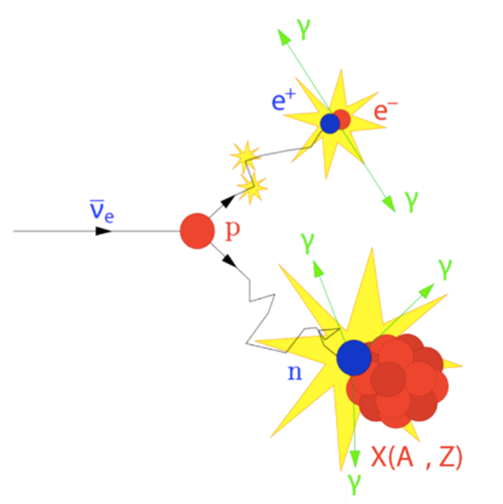
\includegraphics[width=0.5\linewidth]{Chapter2/Figs/Raster/inverse_beta_diagram.png} 
  \captionof{figure}{A diagram of inverse $\beta$ decay 
 (equation \ref{inverse_beta_decay}). The neutrons random walk means it will take (O $\sim$ 10 $\mu$s) before it is detected but the positron emission is prompt. From \cite{ibdPictureLink}.}
  \label{fig:inverse_beta_diagram}
\end{figure}

In a reactor $\sim$ 200\,MeV is released per fission and $\sim$ 6 neutrinos along the $\beta$ decay chain are produced \cite{Mueller_2011}. ``Since unstable fission products are neutron-rich nuclei all $\beta$ decays are of $\beta^-$ type and the neutrino flux is actually pure electronic $\bar{\nu}$s ($\bar{\nu_e}$)''\cite{Mueller_2011}, meaning that the $\bar{\nu_e}$s are the main particles of interest for reactor studies. Neglecting the small kinetic energy of the neutron, the kinetic energy of the positron may be related to the $\bar{\nu}$ via equation \ref{nu_energy_eq}. Which shows the $\bar{\nu_e}$ energy in terms of well known quantities, the kinetic energy and rest mass of the $e^+$ and the masses of the neutron and proton \cite{Vogel_1999}. 
\begin{equation}
 E_{\bar{\nu_e}} = T_{e^+} + m_{e}c^2 + (m_n - m_p)c^2  %E_{e^+} + (M_n - M_p) 
\label{nu_energy_eq}
\end{equation}

\section{$\bar{\nu}$ Reactor Monitoring}
% Obviously the two papers to mention here are vogal and beacom 1999 \cite{Vogel_1999} and muller et al 2011 \cite{Mueller_2011}. They cover the ground pretty well. \cite{Mueller_2011} has the $10^{20}$ $\Bar{\nu_e}$/s per GW$^{Th}$ and \cite{Vogel_1999} has the cross section values. \cite{Vogel_1999} is mostly dealing with stuff to first order, it may be worth addressing how this changes with increasing order. But probably not considering the low number of events $\bar{\nu}$ detection yields. Worth also going over the cowan and riens \cite{Cowan1956Confirmation} \cite{cowan1957test} again just briefly. The songs s1 project is also a necessity in 2007 it marked the beginning of serious reactor monitoring \cite{Bowden_2007}. And of course the original soviet paper which suggested this is as a possibility \cite{Borovoi_1978}. Also need to mention the IAEA and there workshop which suggested the limitations for this \cite{IAEA_2008}. 
% \\\\Probably best to go onto semi chronologically with the Cowan and Reins approach stating that reactor monitoring was one of the original approaches as fuel decays through beta decay (equation \ref{modern_beta_decay}) and the detection occurs through equation \ref{inverse_beta_decay}. It may be worth also mentioning section \ref{Direct_Measurements_section}. Then mentioning the soviet paper \cite{Borovoi_1978} then the move on to the first prototype with SONGS1 and then \cite{Bowden_2007} which then informed the IAEA report \cite{IAEA_2008}. Then talk about vogel \cite{Vogel_1999} and muller \cite{Mueller_2011}.
In 1978 it was proposed that measuring $\bar{\nu}$s from reactors could be used for reactor monitoring \cite{Borovoi_1978}. However, due to the geopolitics of the time, the interest in non-proliferation was not as high as in modern times. It took until 2007 for the SONGS1 prototype to be deployed as proof of concept for reactor monitoring \cite{Bowden_2007}.
%Reactor monitoring was used to prove the existence of neutrinos. In 1953 the direct measurements of $\bar{\nu_e}$ from reactors was done by Cowan and Reins \cite{Cowan1956Confirmation}. The response of $\bar{\nu}$s was measured in cadmium-doped liquid scintillator \cite{Cowan1956Confirmation} which used inverse $\beta$ decay (equation \ref{inverse_beta_decay}). This will be expanded upon in section \ref{Direct_Measurements_section}. $\sim$ 20 years after that experiment %in 1978 it was proposed that measuring $\bar{\nu}$s from reactors could be used for reactor monitoring \cite{Borovoi_1978}. However, due to the geopolitics of the time, the interest in non-proliferation was not as high as in modern times. It took until 2007 for the SONGS1 prototype to be deployed as proof of concept for reactor monitoring \cite{Bowden_2007}. 
\\\\After the deployment of the SONGS1 prototype the International Atomic Energy Agency (IAEA) workshopped a list of positive traits that they would like to see in an $\bar{\nu}$ reactor monitoring detector. These traits include inert construction, non-liquid, easy operation, cheap, portable, robust, above-ground operation, and easy deployment \cite{IAEA_2008}. Whilst these are not requirements, all of these traits can be met in a single detector. For example, VIDARR and RMon meet all of these traits. As they were purpose built to do so. 
\\\\For reactors that operate for long periods without refuelling, $\bar{\nu}$ monitoring has the potential to correlate the measured spectra with build up of $^{239}$Pu in the core, and determine when and how often refuelling occurs. This information is useful for non-proliferation purposes. However, this is not possible for reactors that may refuel online such as Advanced Gas-Cooled Reactors (AGRs) and pebble bed reactors.
% \\\\Reactors produce O $\sim$ $10^{20}$ $\Bar{\nu_e}$/s per GW$^{Th}$ as the fission products in the fuel elements $\beta$ decay \cite{Mueller_2011}. Though these rates are very high, the interaction cross-section to first order is $\sim 10^{-42}$cm$^2$ as can be seen in figure \ref{mullerAndVogelCombined} \cite{Vogel_1999}. In addition to this different fission, fractions will decay at different rates as can be seen in figure \ref{mullerAndVogelCombined}. The combination of these two effects can be seen in figure \ref{fig:anSpectraIsotopes} \cite{Mueller_2011}. From figure \ref{fig:anSpectraIsotopes} the range of $\bar{\nu}$ energies expected to be detected ranges from $\sim$ 1.8\,MeV to $\sim$ 8.5\,MeV. The threshold is 1.804\,MeV as this is the mass difference between the initial and final states \cite{Mueller_2011}. The true threshold energy of the reaction is slightly higher 1.806\,MeV, as the relativistic neutrino momentum requires the neutron and $e^+$ to have some momenta \cite{Vogel_1999}. Immediately after an IBD, the positron will annihilate giving two 511\,keV $\gamma$-rays and the neutron will thermalise in the detector medium before capture. The time taken for thermalisation causes a characteristic double coincidence signal with a delay between a prompt signal from positron interactions and the later neutron capture. This double coincidence may be used to select IBD events from background events. Dependent on the detector media, the mean time between positron and neutron signals is 10\,$\mu$s -- 100\,$\mu$s.

% \begin{table*}[!h]
% \centering
% \begin{tabular}{ll}  
% %\toprule
% %\midrule
% 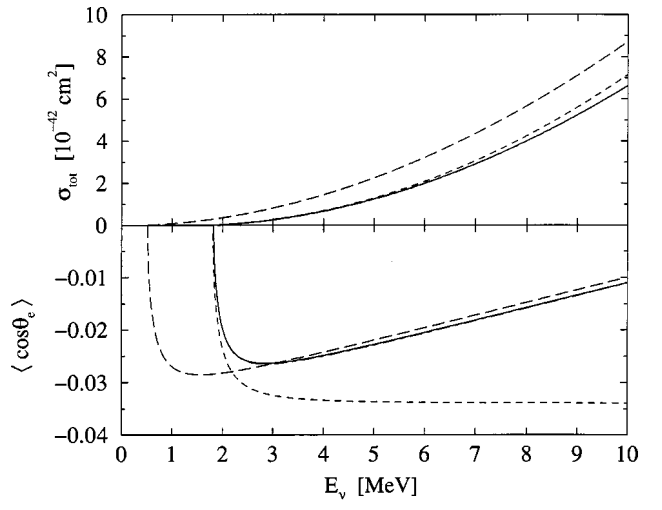
\includegraphics[width=0.49\linewidth]{Chapter1/Figs/Raster/vogelAndBeacomCrossSection.png} &    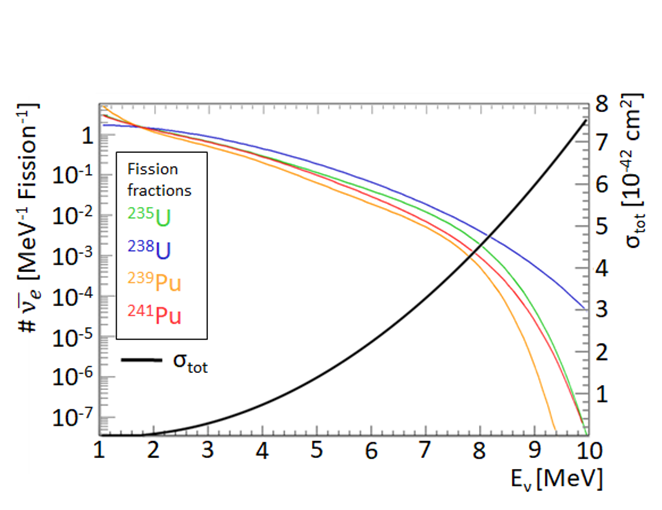
\includegraphics[width=0.49\linewidth]{Chapter1/Figs/Raster/mullerAndVogelCombined.png}\\
%  Upper panel: total cross-section for Inverse $\beta$ decay; bottom panel: $\bra{}\cos(\theta)\ket{}$ for the same reaction; both as a function of the $\bar{\nu}$ energy. The solid line is the O(1/M) result and the short-dashed line is the O(1) result. The long-dashed line is the result of Eq. 3.18. From \cite{smith_1972} \cite{Vogel_1999}. a & fig b\\
% %\bottomrule  
% \end{tabular}
% %\caption{a table figure test}
% \label{tab:figTest}
% \end{table*}

\begin{figure}[!h]
\centering
\begin{minipage}{.45\textwidth}
  \centering 
  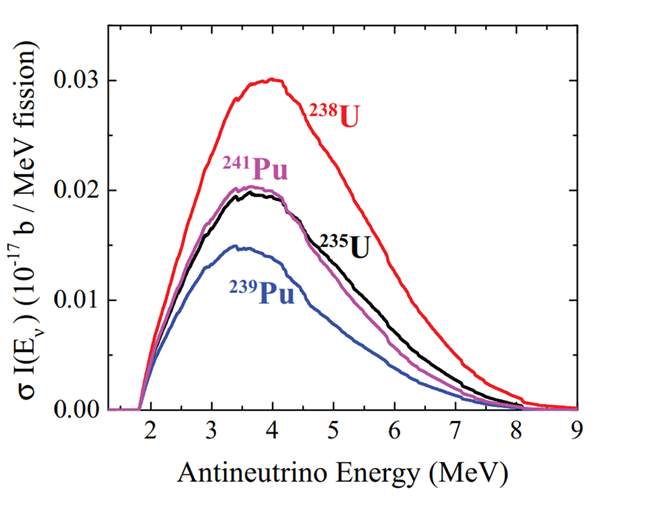
\includegraphics[width=\linewidth]{Chapter1/Figs/Raster/detectedNueSpectrumMultipleIsotopes.png}
  \captionof{figure}{$\bar{\nu}$ spectra multiplied by the $\bar{\nu} + p \rightarrow n + e^+$ cross section for the thermal fission of $^{235}$U and $^{239,241}$Pu and the fast fission of $^{238}$U. From \cite{sonzogni_nucStrcutre_2015}.} 
  \vspace{0.478cm} %1 line = 0.478cm % 2 lines = 0.956cm % 3 lines= 1.434cm % 4 lines = 1.912cm % 5 lines = 2.39cm
  \label{fig:anSpectraIsotopes}
  \end{minipage}
  \qquad
\begin{minipage}{.45\textwidth}
  \centering
  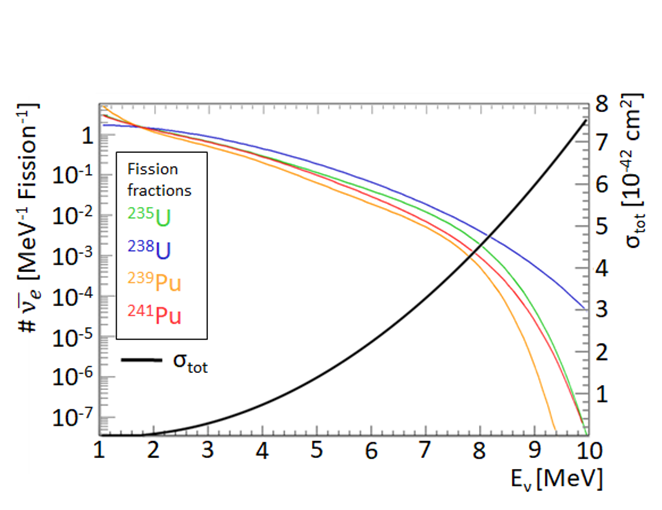
\includegraphics[width=\linewidth]{Chapter1/Figs/Raster/mullerAndVogelCombined.png} 
  \captionof{figure}{A combination of the fission fractions from \cite{Mueller_2011} and the first-order approximation of the cross-section from \cite{Vogel_1999} and their evolution over the energy range where the two distributions cross over.}
  \label{mullerAndVogelCombined}
\end{minipage}%
\end{figure}

% \begin{figure}[!h]
%  \centering
%  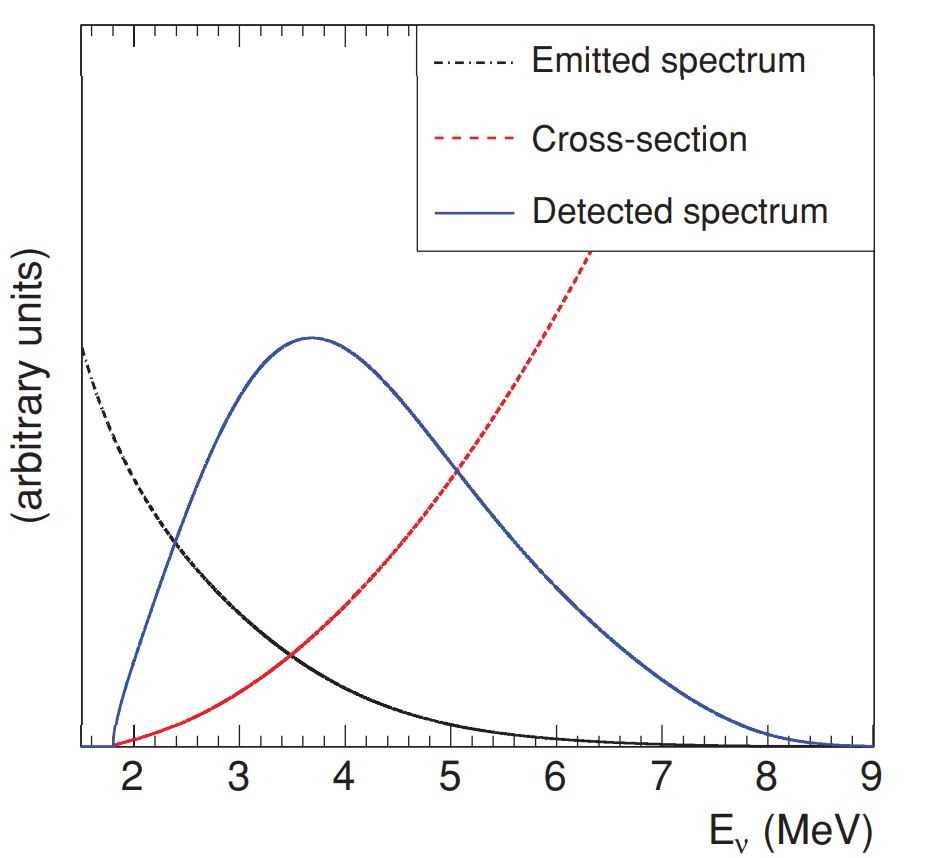
\includegraphics[width=0.4\linewidth]{Chapter1/Figs/Raster/mullerEtAlDetectedSpectrum.png} %height of this plot had to be adjusted because of its unusal diemensions
%  \captionof{figure}{Detected $\bar{\nu}$ spectrum for $^{235}$U fission (blue solid curve). Units are arbitrary and oscillation effects are suppressed. The detected rate rises from the threshold value at about 1.8\,MeV, reaches a maximum around 4\,MeV, and vanishes after 8\,MeV. This shape is the result of folding the emitted spectrum (black dashed-dotted curve), parametrization taken from \cite{Mueller_2011} inverse $\beta$ cross-section (red dashed curve). From \cite{Mueller_2011}} %~can be used as a kind of place holder in latex
%  \label{mullerEtAlDetectedSpectrum}
% \end{figure}

%It may be possible to discern the different fission fraction isotopes from their detected spectra. Providing the energy resolution, statistics, and location of the detector is sufficient. This would be very useful for non-proliferation purposes as measuring the $^{239}$Pu burn-up would lead to a more accurate measure of weapons-grade material than measuring on/off cycles. As online refuelling methods seen in reactors such as the Advanced Gas-cooled Reactors (AGRs) would not work around the measurement of $^{239}$Pu burn-up. The AGR reactor type can refuel online without shutting down. Therefore measure the reactor on/off cycle may not be sufficient for that specific reactor type. This is also true for other types such as pebble beds. As such the measurement of $^{239}$Pu burn-up is desirable. 

\subsection{Reactor $\bar{\nu}$ spectra}
$\sim$ 800 isotopes produced by nuclear reactors $\beta-$ decay and so contribute to $\bar{\nu}$ flux \cite{sonzogni_nucStrcutre_2015}. As each fissioning isotope populates the $\beta$ decaying isotopes differently, the expected $\bar{\nu}$ spectra for the 4 main fissioning isotopes $^{235,238}$U, $^{239,241}$Pu are not identical. The calculated $\bar{\nu}$ spectra produced by Sonzogni et. al. \cite{sonzogni_nucStrcutre_2015} is shown figure \ref{fig:anSpectraIsotopes}. The range of $\bar{\nu}$ energies expected to be detected ranges from $\sim$ 1.8\,MeV to $\sim$ 8.5\,MeV approximately following a exponential drop-off with energy. Above the detection threshold, $^{235}$U and $^{238}$U produce more $\bar{\nu}$s per fission overall than $^{239}$Pu and $^{241}$Pu and there is also a difference in the energy dependence with U isotopes producing harder $\bar{\nu}$s than Pu isotopes. To determine a measurable difference between isotopes, the IDB cross-section needs to be considered. This is also shown in fig \ref{mullerAndVogelCombined}, taken from calculations in \cite{Vogel_1999}. As the IBD cross-section increases with energy, the $\bar{\nu}$ flux decreases, leading to the interaction rate in a detector peaking at $\sim$ 4\,MeV for $^{235}$U, shown in figure \ref{fig:anSpectraIsotopes}.
%With knowledge of the output power of a reactor, $\bar{\nu}$ monitoring has the potential to determined the dominant fissioning isotopes 235U/239Pu and monitor evolution of the core from measurement of the total neutrino flux. By measurement of the $\bar{\nu}$ spectrum, prior knowledge of the power output of the reactor is not necessary.

\subsection{SONGS1 Detector}
The SONGS1 detector \cite{Bowden_2007} was the first $\bar{\nu_e}$ detector to be deployed and prove the technology was viable for non-proliferation purposes. The detector consists of three subsystems; a central detector containing the Gd-doped liquid scintillator target and photomultiplier tube (PMTs), a passive water or polyethylene shield on all sides and a plastic scintillator $\mu$ veto placed outside the water shield on 5 sides of the detector. The central detector seen in figure \ref{fig:SongsS1Detector} consists of four identical stainless steel cells with 0.64 tons of liquid scintillator in total \cite{Bowden_2007}. 
\\\\The SONGS1 detector had a stand off from the reactor core of 24.5 $\pm$ 1\,m \cite{Bowden_2007}. With the 0.64 ton detector a neutrino rate of 407 $\pm$ 75/day was expected according to the SONGS1 collaboration \cite{Bowden_2007}. Figure \ref{subFig:reactorPowerSongsS1} shows the measured $\bar{\nu}$ rate at switch on the reactor, matching the expected rate within error. Figure \ref{subFig:reactorRefulingSongs1} shows the $\bar{\nu}$ rate, over a longer time period encompassing a refuelling cycle. The $\bar{\nu}$ rate is shown to drop with time during periods of constant power output of the reactor, following the predicted change in $\bar{\nu}$ rate due to fuel evolution \cite{Bowden_2008}. Increasing the averaging time to 30 days allowed for the observation of fuel burn-up (see figure \ref{subFig:reactorRefulingSongs1}) \cite{Bowden_2008}. This presents a tantalising opportunity that other collaborations might be able to expand upon with improved energy resolution and event selection. But whether quantifying fuel burn-up is possible with reactor monitoring remains to be seen at time of writing. 

\begin{figure}[!h]
 \centering
 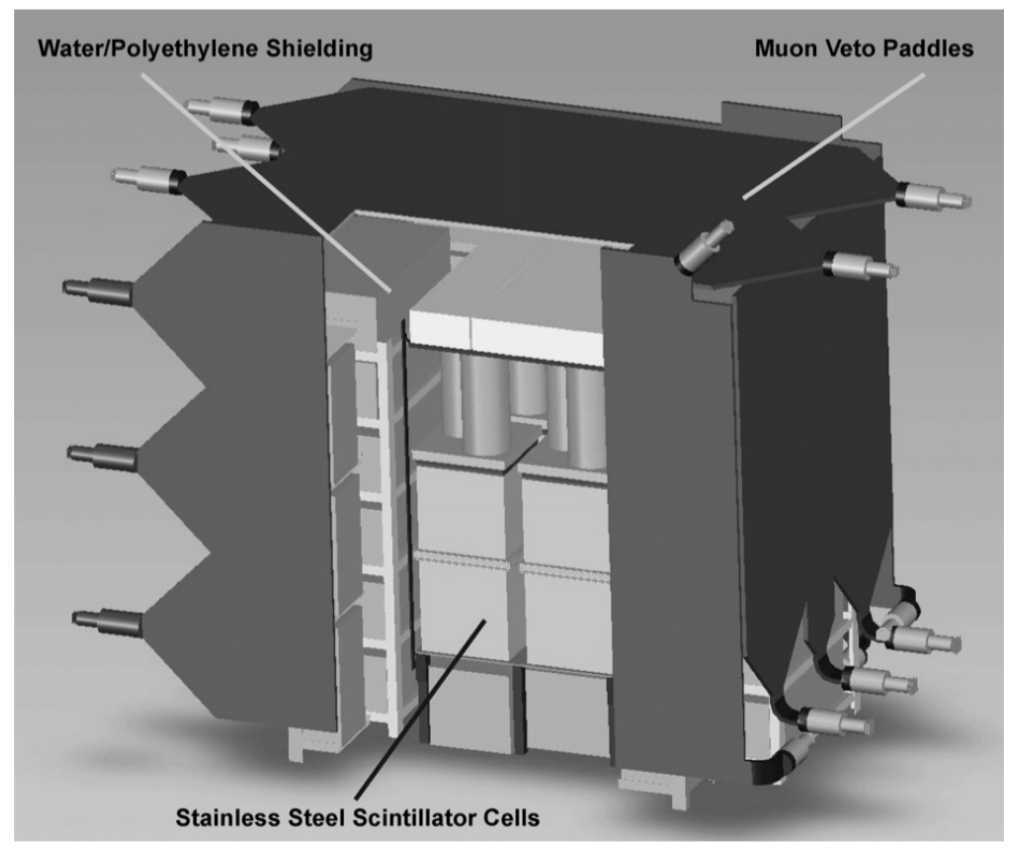
\includegraphics[width=0.5\linewidth]{Chapter1/Figs/SongsS1Detector.jpg}
 \captionof{figure}{A cut away diagram of the SONGS1 detector, showing the major subsystems. From \cite{Bowden_2007}.} 
 \label{fig:SongsS1Detector}
\end{figure}

\begin{figure}[!h]
\centering
\begin{subfigure}{.5\textwidth}
  \centering
  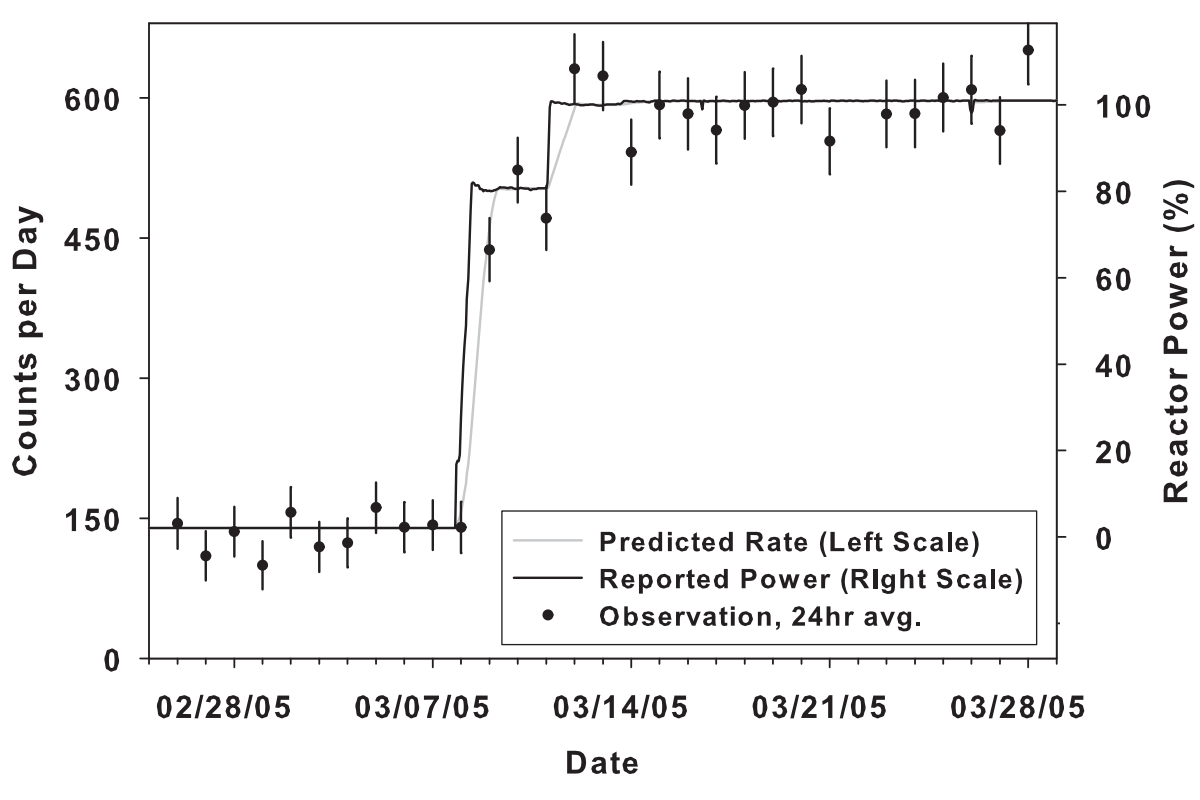
\includegraphics[width=\linewidth]{Chapter1/Figs/reactorPowerSongsS1.png}
  \captionsetup{width=.9\linewidth}
  \caption{}
  \label{subFig:reactorPowerSongsS1}
\end{subfigure}%
\begin{subfigure}{.5\textwidth}
  \centering
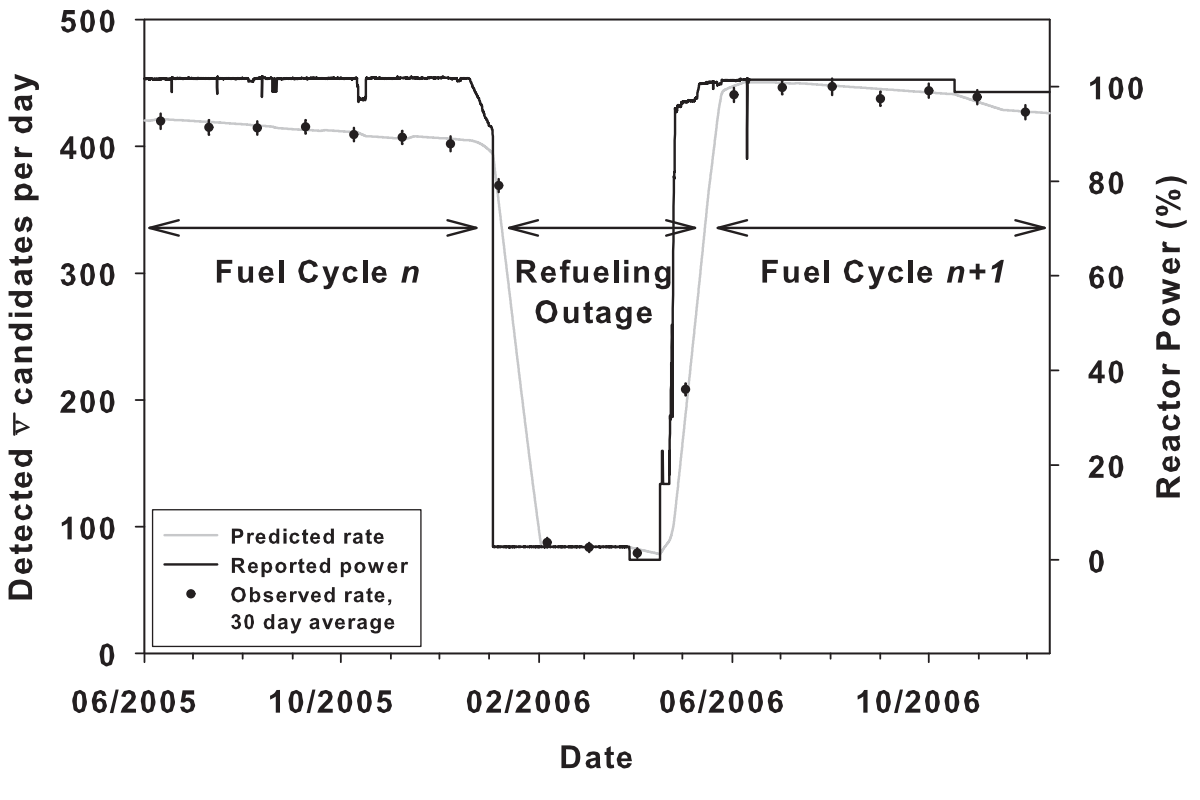
\includegraphics[width=\linewidth]{Chapter1/Figs/reactorRefulingSongs1.png}
  \captionsetup{width=.9\linewidth}
  \caption{}
  \label{subFig:reactorRefulingSongs1}
\end{subfigure}
\caption{Reactor Power and measured $\bar{\nu_e}$ from the SONGS1 core at reactor on in (a) and refuelling in (b). The measured rate approximates power well. From \cite{Bowden_2008}.}
\label{fig:reactorPowerAndRefuelingSongsS1}
\end{figure}

\subsection{PANDA}
The Plastic Anti-Neutrino Detector Array (PANDA) \cite{PANDA_2012}, \cite{PANDA_2014}, \cite{PANDA_tgf}, \cite{IIRIE_Panda_2021}, is a segmented detector that uses plastic scintillator bars and gadolinium embedded in-between the bars shown in figure \ref{subFig:pandaClose}, the gadolinium's interaction with neutrons is shown in equation \ref{equ:gadolinumNAbsorption}. Bars orientations can be seen in figure \ref{subFig:pandaFar} with each layer of bars parallel to each other. The bars have dimensions of 10\,cm$\times$10\,cm$\times$100\,cm with two 10\,cm$\times$10\,cm$\times$10\,cm acrylic cubic light guides glued to both ends of the plastic scintillator with optical cement capped with PMTs at either end of the bars for data collection with Gd doped sheets inserted between bars \cite{PANDA_2014}. The interior of a plastic scintillating bar can be seen in figure \ref{subFig:pandaClose} which also shows the prompt and delayed event of an $\bar{\nu_e}$ event. In addition calibrations and comparison to GEANT4 \cite{Agostinelli:2002hh} have been performed with a baseline of a $^{60}$Co with reasonable agreement between the calibration source and the simulated response \cite{PANDA_2012}. 

\begin{equation}
n + {^{155,157}Gd} \rightarrow {^{156,158} Gd} + \gamma (\sim 8\,MeV)
\label{equ:gadolinumNAbsorption}
\end{equation}

\begin{figure}[!h]
\centering
\begin{subfigure}{.5\textwidth}
  \centering
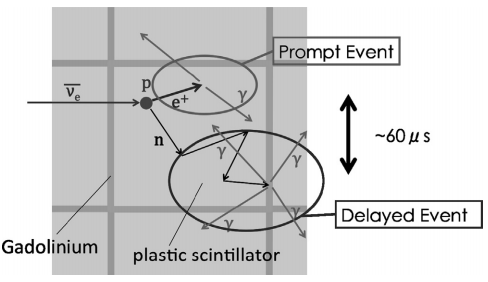
\includegraphics[width=\linewidth]{Chapter2/Figs/Raster/Panda_close.png}
  \captionsetup{width=.9\linewidth}
  \caption{}
  \label{subFig:pandaClose}
\end{subfigure}%
\begin{subfigure}{.5\textwidth}
  \centering
  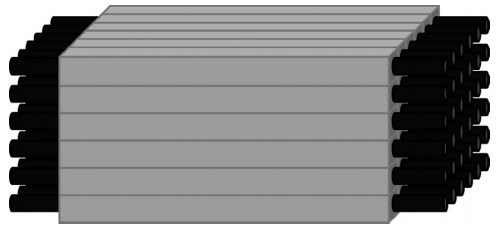
\includegraphics[width=\linewidth]{Chapter2/Figs/Raster/Panda_far.png}
  \captionsetup{width=.9\linewidth}
  \caption{}
  \label{subFig:pandaFar}
\end{subfigure}
\caption{The interior is shown in (a) which also shows a  $\bar{\nu_e}$ interaction with prompt and delayed components. The exterior of PANDA is shown in (b). The bars are clustered together with photon multiplier tubes at the end to measure photons. From \cite{PANDA_2014}.}
\label{fig:pandaCloseFar}
\end{figure}

%The bars are not positioned perpendicularly in the $z$ direction (figure \ref{subFig:pandaFar}). Therefore tracking is more difficult in PANDA, due to not having specific $x$ and $y$ coordinates, this makes vetoing cosmic $\mu$ (a major source of background) potentially harder in PANDA than if the bars were perpendicular. 
%The photon multiplier tubes (PMTs) used in PANDA are also expensive, the PANDA36 shown in figure \ref{subFig:pandaFar} is much smaller than the proposed final design of 100 channels and 1m$^3$ \cite{PANDA_2012} but PANDA is being built in stages because of the expense of these components. However, the potential for measuring many photons with high efficiency makes PMTs attractive. Both Lesser PANDA (16 channels) and PANDA36 have been deployed by van with background measurements and reactor measurements being taken from inside the van \cite{PANDA_2012}, \cite{PANDA_2014}. But due to the flammable nature of petrol and diesel, it is unclear whether reactor operators would be open to having a van stationed indefinitely outside their reactor buildings. PANDA36 has also been used for monitoring Terrestrial $\gamma$-ray Flashes (TGFs) from thunderstorms to allow for further background reduction at nuclear sites\cite{PANDA_tgf}.
Owing to the cost of PMTs, PANDA has been built in stages.  Both Lesser PANDA (16 channels) and PANDA36 have been deployed by van with background measurements and reactor measurements being taken from inside the van \cite{PANDA_2012}, \cite{PANDA_2014}. For example, PANDA36 has been used for monitoring Terrestrial $\gamma$-ray Flashes (TGFs) from thunderstorms to allow for further background reduction at nuclear sites\cite{PANDA_tgf}. In 2016 PANDA was upgraded to its final size, 100 channels. The PANDA100 detector started taking measurements at the Ohi power plant in 2018 for background subtraction and then made measurements of the neutrino events in 2019 from Ohi reactors 3 and 4, at a standoff of 45\,m and 100\,m from the reactor cores \cite{Iwata_2019}. The results of the neutrino measurements from the reactors is shown in figure \ref{subFig:Panda_spectrumOfIbdCandidates} and the background spectrum is shown in \ref{subFig:Panda_SpectrumOfCosmicProducts}. The results from PANDA's deployment are very impressive with an $\bar{\nu}$ rate of 175.8 $\pm$ 34.4 day$^{-1}$ \cite{IIRIE_Panda_2021}. Of particular interest in the PANDA results is the neutrino spectrum produced in figure \ref{subFig:Panda_spectrumOfIbdCandidates} as it resembles the expected shape from Muller 2011 \cite{Mueller_2011} and by Sonzogni \cite{sonzogni_nucStrcutre_2015} (see figure \ref{fig:anSpectraIsotopes}).

\begin{figure}[!h]
\centering
\begin{subfigure}{.4\textwidth}
  \centering
  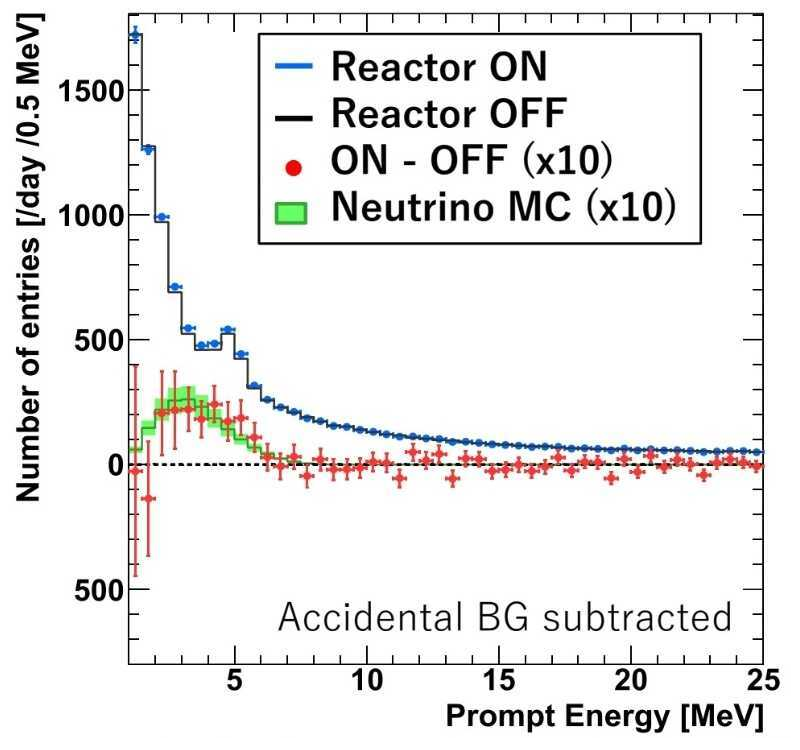
\includegraphics[width=\linewidth]{Chapter1/Figs/Panda_spectrumOfIbdCandidates.png}
  \captionsetup{width=.9\linewidth}
  \caption{}
  \label{subFig:Panda_spectrumOfIbdCandidates}
\end{subfigure}%
\begin{subfigure}{.4\textwidth}
  \centering
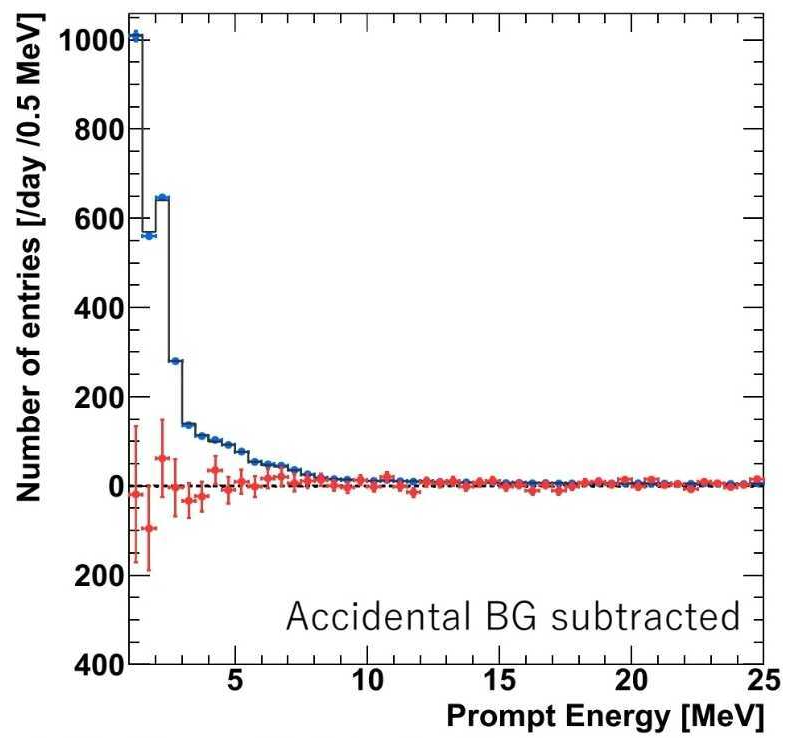
\includegraphics[width=\linewidth]{Chapter1/Figs/Panda_SpectrumOfCosmicProducts.png}
  \captionsetup{width=.9\linewidth}
  \caption{}
  \label{subFig:Panda_SpectrumOfCosmicProducts}
\end{subfigure}
\caption{Results from the PANDA deployment between 2018 -- 2019. In (a) Number of observed neutrinos is 175.8 $\pm$ 34.4 [day$^{-1}$] to within 5.10 $\sigma$. In (b) the spectrum of cosmic products is shown to go to zero once accounting for background. From \cite{IIRIE_Panda_2021}.}
\label{fig:Panda_spectrumOfIbdAndCosmicCandidates}
\end{figure}

% \subsection{SoLid and CHANDLER}
% The SoLid detector is a plastic scintillating detector that uses wavelength shifting (WLS) fibres with MPPCs at the end to read out fibre signals and adjacent 5\,cm $\times$ 5\,cm $\times$ 5\,cm cubes being lit up at similar time intervals to discern particles \cite{Solid_proposal}. There is a prompt signal outputted from the positron in the plastic cubes and a delayed signal from the $^6$LiF:ZnS(Ag) screen interacting with neutrons as shown in figure \ref{fig:SolidCubeDiagram}. The prompt positron response and delayed neutron response is similar to the other experiments mentioned. In SoLid $^6$Li is used as the neutron capture agent (equation \ref{Li_interact_eq}), which produces an $\alpha$ and a 4.78\,MeV $\gamma$ \cite{Solid_readout}. The $\gamma$ signal is ignored because the $\alpha$ signal produced is clear and produces a specific pulse shape signal \cite{Solid_readout} which has a very minimal background due to its specific pulse shape. Setting it apart from other experiments that use the 8\,MeV Gd cascade. 

% \begin{equation}
% n + {^6Li} \rightarrow {^3H} + \alpha +4.78\,MeV
% \label{Li_interact_eq}
% \end{equation}

% \begin{figure}[!h]
%  \centering
%  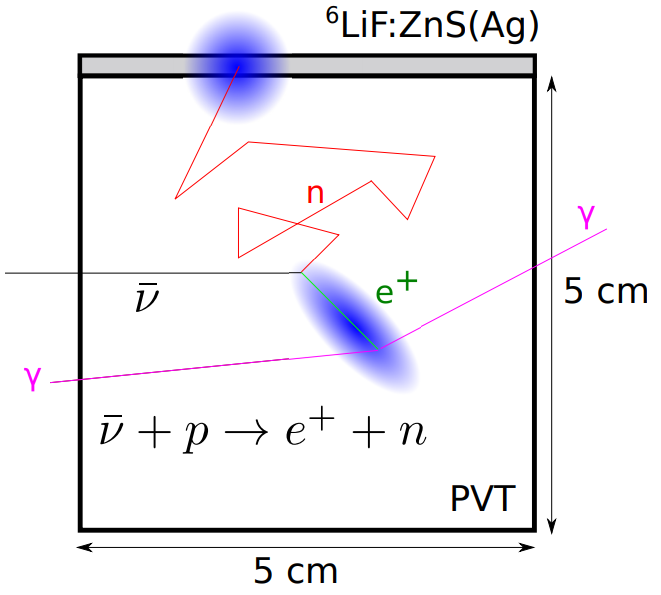
\includegraphics[height=58mm]{Chapter2/Figs/Raster/SoLid_cube.png}
%  \captionof{figure}{SoLid cube during an inverse beta decay event $\bar{\nu}$ decays into a positron and neutron via equation \ref{inverse_beta_decay}, delayed neutron is captured by $^6$LiF:ZnS(Ag) screen, positron gives the prompt response. From \cite{Solid_readout}.} 
%  \label{fig:SolidCubeDiagram}
% \end{figure}

% The challenge with using $^6$Li as a neutron capture agent is producing enough light for pulse shape discrimination (PSD) to be used in the analysis. The $\alpha$s need to be captured by the sulphur in the $^6$LiF:ZnS(Ag) screen which then emits a specific $\gamma$ into the plastic which in turn produces electrons via Compton scattering which are then captured by WLS fibres. An alternative method to this is that proposed by CHANDLER (Carbon Hydrogen $\bar{\nu}$ Detector with a Lithium Enhanced Raghavan-optical-lattice) \cite{aap2015}. Which uses PMT's and a Raghavan-optical-lattice to counter-act the low light issues in SoLid. However, the CHANDLER design also brings challenges as the detector cannot be too large otherwise attenuation and containment of events prevent signals from being read.
% \\\\The SoLid experiment has collected data up to June 2020 and is current deployed at the BR2 reactor in Belgium [6300 mm–8938 mm] from the nominal reactor core \cite{Abreu_2021}. The results from the period of July 2018 -- August 2019. The trigger strategy for for SoLid neutrinos relies solely on triggering on a scintillation signal generated in the
% neutron detection screens (NS). The values for the NS rate for SoLid at BR2 can be seen in figure \ref{fig:solidReults}. As such figure \ref{fig:solidReults} shows how the SoLid detector is triggering as expected for an $\bar{\nu}$ detector. Currently the SoLid collaboration approximates the detector is subject to $\sim$ 1000 per day though the short bursts the BR2 causes difficulty through off-equilibrium effects \cite{Abreu_2021}. 
% \begin{figure}[!h]
%  \centering
%  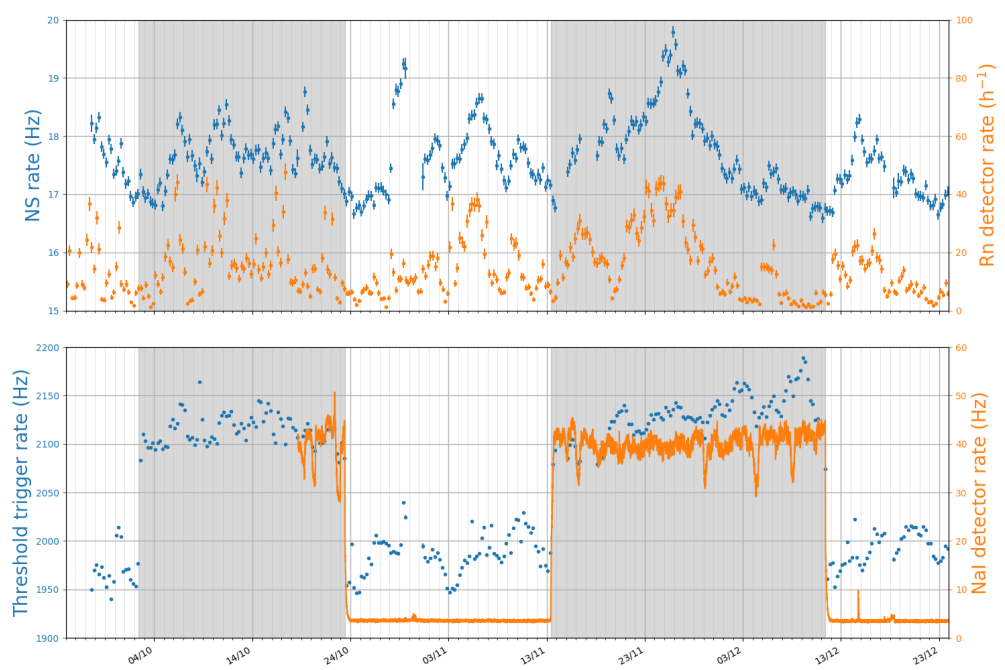
\includegraphics[width=0.7\linewidth]{Chapter1/Figs/SoLidResults.png}
%  \captionof{figure}{Results from SoLid detector at BR2. (Top) Long term trends of the NS rate after muon contamination removal (blue) and the airborne radon detector rate (orange). (Bottom) Long term trends of the threshold trigger rate (blue) and the NaI detector rate (orange). Reactor ON periods are shown as grey bands. From \cite{Abreu_2021}} 
%  \label{fig:solidReults}
% \end{figure}

\subsection{RENO} \label{subSec:reno}
%Papers found by this collaboration include \cite{reno_may_2012}, \cite{reno2013},  \cite{reno_may_2019}. 
RENO was the first long base line experiment to see $\Bar{\nu_e}$ disappearance \cite{Olive_2014}. The RENO experiment consists of two detectors at a distance of 408.56\,m for the near detector, and 1443.99\,m for the far detector \cite{reno_may_2012}. A schematic of the detectors used in RENO can be seen in figure \ref{fig:RENO_detector}, this detection system uses Gd-doped liquid scintillator with PMTs. By measuring the prompt energy from both the near and far RENO detectors a spectrum of energies for both can be produced (figure \ref{fig:RENO_Spectrum}). There is a clear $\bar{\nu_e}$ disappearance visible between the near and far detector spectra in figure \ref{fig:RENO_Spectrum} \cite{reno_may_2012}. Figure \ref{fig:RENO_Spectrum} also shows the ratio between the near and far detectors further highlighting the neutrino deficit. 

\begin{figure}[!h]
\centering
\begin{minipage}{.45\textwidth}
  \centering
  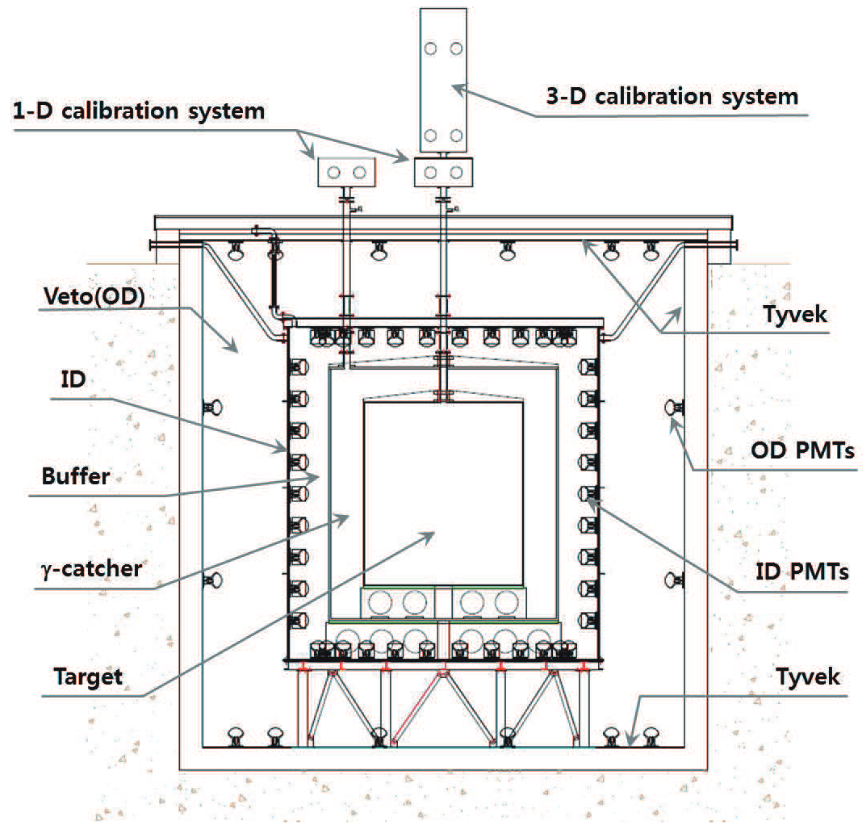
\includegraphics[width=\linewidth]{Chapter2/Figs/Raster/RENO_detector.png}
  \captionof{figure}{schematic view of a RENO detector. The near and far detectors are identical. The detector seen in this figure consists of a main inner detector (ID) and an outer veto detector (OD) from \cite{reno_may_2012}.} 
  \label{fig:RENO_detector}
  \vspace{2.39cm} %1 line = 0.478cm % 2 lines = 0.956cm % 3 lines= 1.434cm % 4 lines = 1.912cm % 5 lines = 2.39cm
\end{minipage}%
\qquad
\begin{minipage}{.45\textwidth}
  \centering
  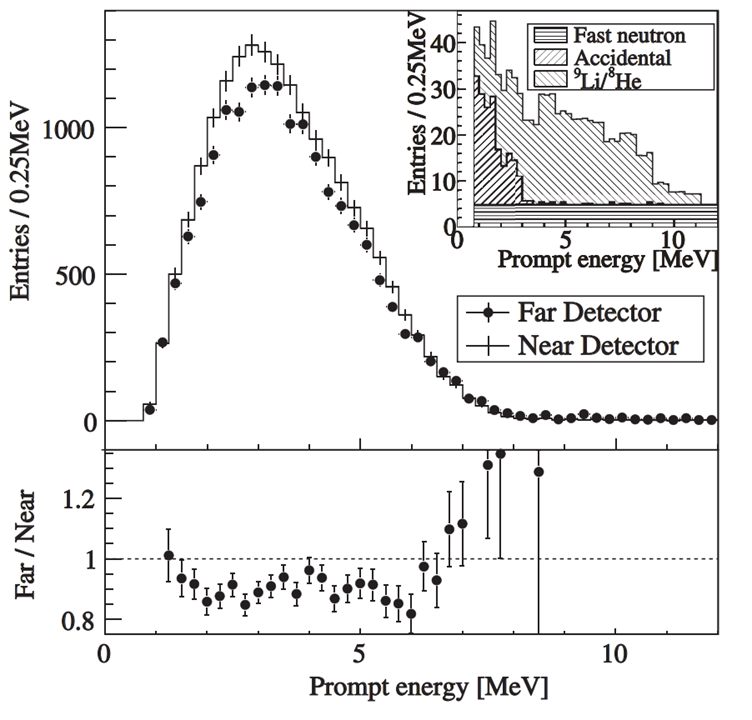
\includegraphics[width=\linewidth]{Chapter1/Figs/Raster/RENO_Spectrum.png} 
  \captionof{figure}{Observed spectrum of the prompt signals in the far RENO
detector compared with the non-oscillation predictions from the measurements in the near RENO detector. The backgrounds shown in the inset are subtracted for the far spectrum. The background fraction is 5.5\,\% (2.7\,\%) for far (near) detector. Errors are statistical uncertainties only. Bottom: The ratio of the measured spectrum of far detector to the non-oscillation prediction. From \cite{reno_may_2012}.}
  \label{fig:RENO_Spectrum}
\end{minipage}
\end{figure}

RENO's results in 2012 were consistent with neutrino oscillations to within 4.9 $\sigma$ from six 2.8\,$GW_{th}$ reactors \cite{reno_may_2012}. RENO was able to constrain the measurement of $\theta_{13}$ (A component Pontecorvo–Maki–Nakagawa–Sakata (PMNS) that will be explained in section \ref{sec:neutrinoFlavours}) in 2012 using a rate based analysis to produce  $\sin^2{2\theta_{13}}$ = 0.113$\pm0.013$(stat.)$\pm0.019$(syst.) which was consistent with the findings that Double Chooz would produce later. These results were revised once again in 2013 using 800 days of live time to $\sin^2{2\theta_{13}}$ = 0.100 $\pm$ 0.010(stat) $\pm$ 0.015 (sys.) corresponding to 6.3 $\sigma$ significance \cite{reno2013}. The focus of the RENO collaboration has since shifted to analysing the 5\,MeV reactor anomaly \cite{reno_may_2019}. 

\subsection{Double Chooz} \label{subSec:doubleChooz}
%I feel like Double Chooz, Reno, KamLAND and Daya Bay are all very similar, liquid scintillating detectors with Gd doping initlally trying to find theta_13 but then transitioned to the 5 MeV reactor bump all of these are not proliforation focussed but measrument focussed experiments 
%Double Chooz is probably one of the most well known reactor monitoring programs. \cite{abe2014improved} goes over some of the details and I have already mentioned it here. Also the \cite{lasserre2006} reference may be useful, used it once before in the first year literature survey. I've also cited \cite{Abe_2012} in the past and that may prove useful here. Further the reference \cite{Olive_2014} may also be of use. Double Chooz is a good one to cite because its clearly not in competition with VIDARR. It requires to be very close and a big hole dug underground and uses gadolinium suspended in liquid organic scintillator. Which is not cheap or portable, it does however give significantly better measurements for the disappearance of $\bar{\nu}$s which the above references mention.

%The Double Chooz experiment is an evolution of the original Chooz experiment which was set up at the Chooz nuclear power plant in France\cite{lasserre2006}. Both of these experiments attempted to measure the $\Bar{\nu_e}$ disappearance from the same reactor however the original Chooz experiment was unable to see any disappearance to a 90$\,\%$ confidence level \cite{Apollonio_2003}. Both experiments used gadolinium doped liquid scintillator with the Double Chooz experiment having a near and far detector at 280\,m and 1050\,m respectively\cite{lasserre2006}. Finally, in 2012 $\Bar{\nu_e}$ disappearance was observed at the Double Chooz experiment \cite{Abe_2012}. These results were improved further in 2014 \cite{abe2014improved}.
The Double Chooz experiment followed the Chooz experiment to measure the disappearance of $\bar{\nu_e}$s from the Chooz nuclear power plant in France \cite{lasserre2006}. With the Chooz experiment failing to measure disappearance to the 90\,\% confidence level \cite{Apollonio_2003}, the upgrade to Double Chooz replaced the detector at standoff of 1050\,m and added a near detector at 280\,m and saw disappearance in 2012 \cite{Abe_2012}. These results were further improved with data taking up to 2014 \cite{abe2014improved}.

\begin{figure}[!h]
 \centering
 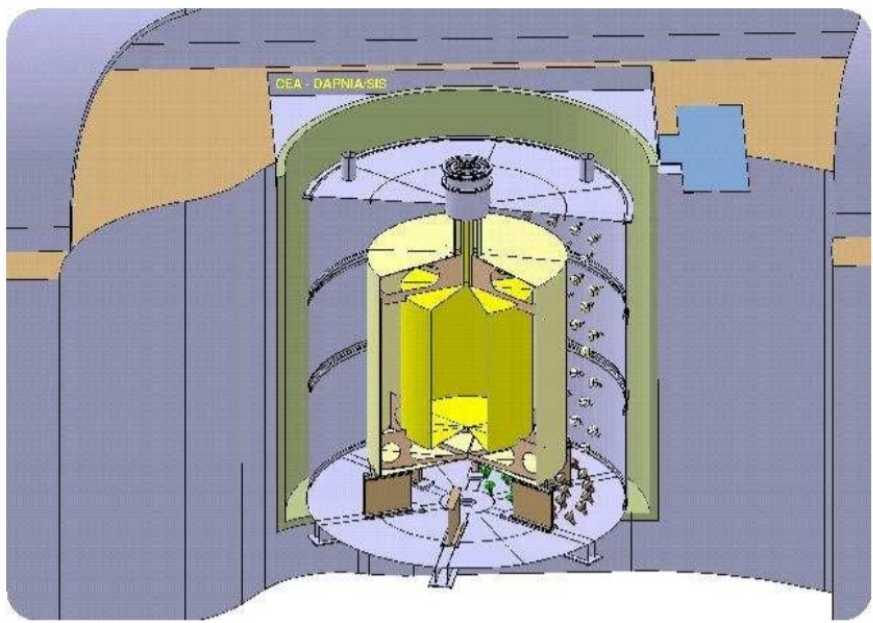
\includegraphics[width=0.5\linewidth]{Chapter1/Figs/doublChoozDetectorDiagram.jpg} %height of this plot had to be adjusted because of its unusal diemensions
 \captionof{figure}{The Double Chooz-far detector at the Chooz underground site (7\,m high and 7\,m in diameter). A total of 10.3\,m$^3$ of dodecane+PXE-based liquid scintillator doped with gadolinium is contained in a transparent acrylic cylinder surrounded by the $\gamma$ region (22.6\,m$^3$) and the buffer (114.2\,m$^3$). From \cite{lasserre2006}.} %~can be used as a kind of place holder in latex
 \label{fig:DoubleChoozFarDetector}
\end{figure}
The Double Chooz experiment uses detectors placed underground to allow for a large amount of overburden to reduce background rates. The overburden for the near detector is 30\,m resulting in 300 water meter equivalent (w.m.e) \cite{lasserre2006}. This high overburden was chosen to keep a high true-neutrino-signal to background ratio. The far detector only has 70-80\,m.w.e and so the outer shielding is different \cite{lasserre2006}. The far detector consists of a 10.3\,m$^3$ volume filled dodecane+PXE based liquid scintillator doped with gadolinium contained in a transparent acrylic cylinder to act of a target, surrounded by a 22.6\,m$^3$ volume to measure background gamma radiations. To minimise background a 114\,m$^3$ buffer region shields the inner-detector. The near and far detectors are identical inside the PMT support structure but the outer shielding is not identical due to the difference in cosmic ray backgrounds at the near and far sites \cite{lasserre2006}. Although the Double Chooz measurement  was not the first to measure the rate of $\bar{\nu}$ disappearance \cite{reno_may_2012} like RENO it was able to produce a spectrum of the disappearance for $\theta_{13}$ which can be seen in figure \ref{doubleChoozSpectrumNoCaption}. The measured energy spectrum (the black points in figure \ref{doubleChoozSpectrumNoCaption}), was best fitted using the parameter of $\sin^2{2\theta_{13}}$ = 0.109 $\pm$0.030(stat)$\pm$0.025(syst) which is shown as the red line in figure \ref{doubleChoozSpectrumNoCaption} \cite{Abe_2012}. The data exclude the no-oscillation hypothesis at 99.8$\%$ CL (2.9$\sigma$)\cite{Abe_2012}. This data was further expanded upon in 2014 producing a result of $\sin^2{2\theta_{13}}$ = 0.090$^{+0.032}_{-0.029}$ using 467.90 live days of data to within $3.0\sigma$ \cite{abe2014improved}.
\begin{figure}[!h]
 \centering
 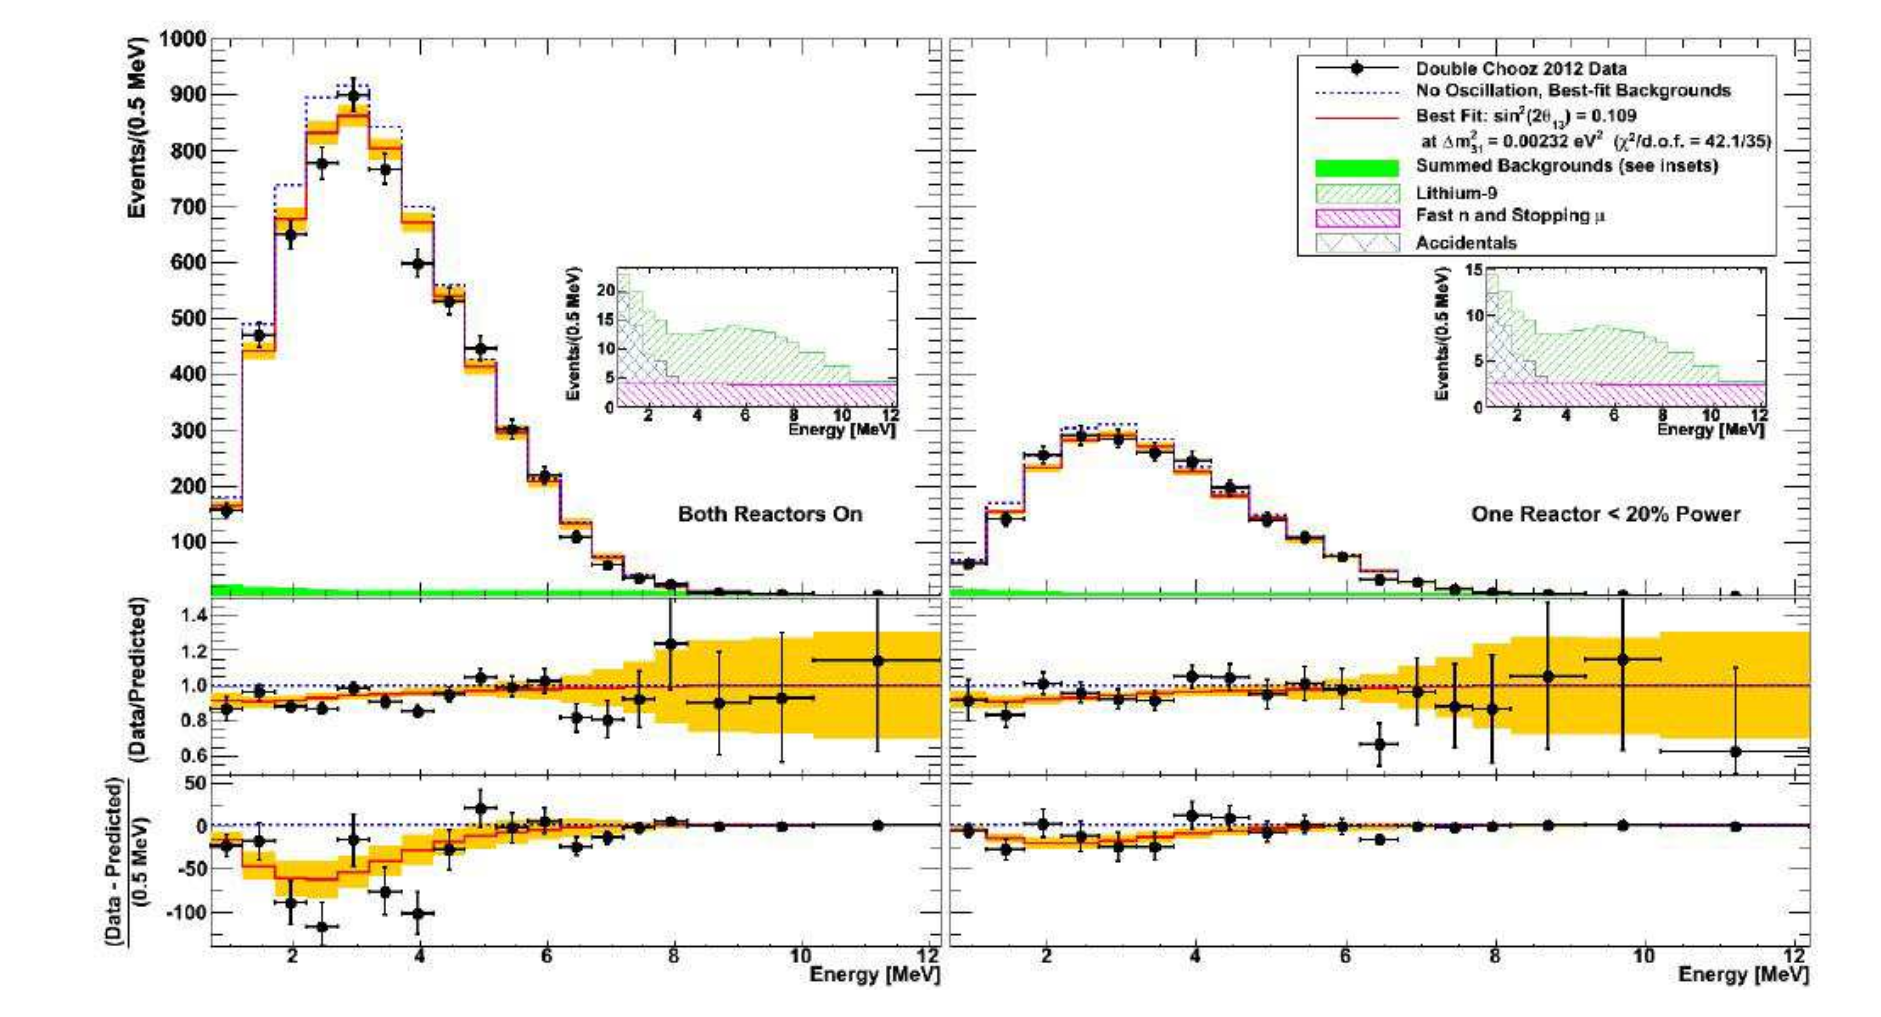
\includegraphics[width=0.8\linewidth]{Chapter2/Figs/Raster/doubleChoozSpectrumNoCaption.png} %Just use linewidth for this one
 \captionof{figure}{Double Chooz measured prompt energy spectrum for each integration period (data points) superimposed on the expected prompt energy spectrum, including backgrounds (green region), for the no-oscillation (blue dotted curve) and best-fit (red solid curve) at $\sin^2{2\theta_{13}}$ = 0.109 and $\Delta$m$^2_{31}$ = 2.32$\times$10$^{-3}$eV$^2$. Inset: stacked spectra of backgrounds. Bottom: differences between data and no-oscillation prediction (data points), and differences between best fit prediction and no-oscillation prediction (red curve).The orange band represents the systematic uncertainties on the best-fit prediction. From \cite{Abe_2012}} %~can be used as a kind of place holder in latex
 \label{doubleChoozSpectrumNoCaption}
\end{figure}

\subsection{Other Experiments}
This list of reactor experiments is not exhaustive near-field examples such as SoLiD \cite{Solid_readout}, CHANDLER \cite{aap2015}, and Nucifer \cite{nucifer2016} were not touched upon. Whilst these experiments may have interesting differences from VIDARR and RMon (both SoLid and CHANDLER use Li instead of Gd and Nucifer is a liquid detector) the utility of these experiments is very similar to the PANDA and SONGS1 examples discussed. The reason SONGS1 was focused on is because it was the first proof of concept for near-field reactor monitoring. Whilst PANDA was focused on as its technology is quite similar to VIDARR's with the near-field ranges of $\sim$ 45\,m -- 100\,m from commercial reactor cores being similar to the expected deployment ranges for VIDARR and the $\sim$ 60\,m range RMon was deployed at. 
\\\\Similarly there are more far-field experiments than Double Chooz and RENO. For example, the Daya Bay experiment in China uses similar technology to both RENO and Double Chooz to measure $\bar{\nu_e}$s from reactors \cite{DayaBay2007Precision}. The Daya Bay experiment has also started to investigate the reactor anomaly at 5\,MeV, similar to RENO \cite{Daya_Bay_2017}. Another experiment of interest is the WATCHMAN collaboration which has the goal of far-field reactor monitoring using $\bar{\nu_e}$s originally planned to be deployed in the U.S.A \cite{askins2015physics} it has since become a joint U.S, U.K project and will be deployed at Boulby mine \cite{burns2018remote}. Its technology is in a state of flux but will use Gd in a fluid detector. There has been some external collaboration between the VIDARR experiment and the WATCHMAN experiment. In particular, the application of the DANCE calorimeter data to form a Dicebox for Gadolinium which VIDARR has also taken advantage of as part of this work. 

%Nucifer is also similar to the other experiments being a scaled-down version of Double Chooz, Daya Bay and RENO using Gd doped liquid scintillator with the goal of near field reactor monitoring \cite{nucifer2016}

% The original prototype to VIDARR deployed at the Wylfa reactor site from June 2014 - Feburary 2016 based on the T2K ND280 ECal was unofficially referred to as RMon by the collaboration. However, the experiment's name has now been finalised as the Verification Instrument for the Direct Assay of Radiation at Range or VIDARR and as such the prototype to VIDARR will be referred to as ProtoV. This naming convention is adopted from the SuperK experiment as the upgrade from Kamiokande to Super Kamiokande is similar in spirit to the upgrade from ProtoV to VIDARR and as such this retroactive naming convention will be applied.
\section{RMon And VIDARR detector for Nuclear Safeguards}
The University of Liverpool has developed a detector to demonstrate the potential usefulness of a $\bar{\nu_e}$ detector for safeguarding purposes. In the modern political climate where nuclear power is seen as a stable form of low carbon power generation, more nations are considering nuclear power once again. As such the concern of atomic weapons proliferation has increased. Current safeguards for non-proliferation are dependent on accurate bookkeeping and estimations from power generation. Whilst these methods are effective, more direct methods of measuring the flux from reactors, and thereby the production of weapons-grade material, would greatly aid international institutions and watchdogs.
\\\\Between 2014 -- 2016 a prototype detector (RMon) based on the T2K ND 280 ECal \cite{Allan_2013} was deployed at the Wylfa reactor site. This deployment proved successful in measuring the reactor on period in 2014. However, there are improvements to the target mass, time resolution, improved Multi-Pixel Photon Counters (MPPCs), and temperature control which would greatly improve these results. An upgrade that implements all of these improvements is in development albeit has experienced delays due to the COVID-19 pandemic. The Verification Instrument for the Direct Assay of Radiation at Range (VIDARR) hopes to provide measurement the $\bar{\nu_e}$ flux with sensitivity and accuracy sufficient for safeguard monitoring whilst fulfilling all the positive traits the IAEA would like to see in a mobile detector \cite{IAEA_2008}.
\\\\In this thesis, the expected performance of the VIDARR detector has been characterised through GEANT4 \cite{Agostinelli:2002hh} simulations to illustrate the potential of the detector. Owing to the high degree of segmentation of the detector compared to other $\bar{\nu_e}$ reactor monitors the tracking of particles especially cosmic $\mu$ through the detector is more accurate. The data taken by the RMon detector at Wylfa has been revisited to demonstrate the detectors capability at cosmic $\mu$ tomography.

% The aim of the Verification Instrument for the Direct Assay of Radiation at Range (VIDARR) project is to demonstrate the potential usefulness of an electron $\bar{\nu}$ ($\bar{\nu_e}$) detector for safeguarding purposes. Between 2014 -- 2016 a prototype detector (RMon) based on the T2K ND 280 ECal \cite{Allan_2013} was deployed at the Wylfa reactor site. This deployment proved successful in measuring the reactor on period in 2014. However, there are improvements to the target mass, time resolution, improved Multi-Pixel Photon Counters (MPPCs), and temperature control which would greatly improve these results. An upgrade that implements all of these improvements is planned and has been characterised through GEANT4 \cite{Agostinelli:2002hh} simulations. In the modern political climate where nuclear power is seen as a stable form of low carbon power generation, more nations are considering the nuclear power once again. As such the concern of atomic weapons proliferation has increased. Current safeguards for non-proliferation are dependent on accurate bookkeeping and estimations from power generation. Whilst these methods are effective, more direct methods of measuring the flux from reactors, and thereby the production of weapons-grade material, would greatly aid international institutions and watchdogs.
% \\\\$\bar{\nu}$ reactor monitoring also has potential benefits for utilising fuel more effectively. Increasing power generation whilst decreasing the amount of nuclear waste to be stored. This potential is not yet fully realised due to the increased complexity of this method as it requires differentiating between different isotopes rather than just measuring reactor $\bar{\nu_e}$ flux. Whether this is feasible will be tested once the upgrades to VIDARR are completed and it is deployed at a new reactor site.  
%!TEX root = ../thesis.tex
%*******************************************************************************
%****************************** Third Chapter **********************************
%*******************************************************************************

% **************************** Define Graphics Path **************************

\ifpdf
    \graphicspath{{Chapter2/Figs/Raster/}{Chapter2/Figs/PDF/}{Chapter2/Figs/}}
\else
    \graphicspath{{Chapter2/Figs/Vector/}{Chapter2/Figs/}}
\fi

%\ref{sec:reactorAntiNeutrinos}

\chapter{Overview of Neutrino Physics}\label{Chp:ABfriefHistoryOfNeutrinos} 
To illustrate the nature and unique properties of the neutrino a historical look at the discovery of the neutrino will be performed in this chapter. This will include the proposal of the neutrino to solve the missing energy in beta decay and the more direct observations in emulsion, as well as an overview of how lepton number and flavour impacted the understanding of the neutrino physics. Then the experimental evidence and theory behind neutrino oscillation will be covered. Finally, how neutrino oscillation might effect reactor neutrino monitoring will be explored. %And the impact of neutrino oscillations on neutrinos and the impact of oscillations on reactor measurements. 

\section{Theoretical Development}
%history of neutrino: \cite{griffiths2008neutrino1.5} \cite{lederman1970resource}
%\\beta decay of tritium (book cannot find, may have to replicate): \cite{lewis1970neutrinos} especially as Fermi mentions it in \cite{Fermi:1934hr}, \cite{wilson1968fermi} 
%\\Neutron proposed by Chadwick in 1932 describing a proton like recoil and odd behaviour of neutrons that can only be described by a neutron or the breaking of conservation of momentum and energy!: \cite{chadwick1932possible}. Important for giving full context to the neutrino discovery
%\\Fermis paper proposing this beta decay after Chadwick's discovery of the neutron is given in \cite{Fermi:1934hr} which proposes a neutrino and is published through Springer and the English translation from 1968 is given in \cite{wilson1968fermi}
%\\So far very little from Pauli need to include him somewhere the neutrino was his idea \cite{lederman1970resource} may have something...
The neutrino was postulated by Pauli in 1931 as a way to conserve both the energy of beta decay and the angular momentum of the products of beta decay  \cite{griffiths2008neutrino1.5}\cite{lederman1970resource}. At the time beta decay was described by equation \ref{oldBetaDecay}. Where $A$ and $B$ represent the decaying particles, as the neutron had not yet been discovered by this point, it was considered a reaction between two nuclei. The conservation of energy dictates that the kinetic energy of the electron should only have a discrete value as shown in equation \ref{constant_ke_e_equation}. However, when the kinetic energy of the electron was measured (see figure \ref{fig:beta_spectrum}) the energy of the electron formed a continuum as seen in figure \ref{fig:beta_spectrum}  \cite{griffiths2008neutrino1.5} \cite{lewis1970neutrinos}. Equation \ref{constant_ke_e_equation} represents the maximum possible energy available to the electron in figure \ref{fig:beta_spectrum} suggesting a third body in beta decay  \cite{griffiths2008neutrino1.5}.


\begin{equation}
    A \rightarrow B + e^-
    \label{oldBetaDecay}
\end{equation}

\begin{equation}
    E = \left( \frac{{m_A}^2 - {m_B}^2 + {m_e}^2}{2m_A}\right) c^2
    \label{constant_ke_e_equation}
\end{equation}

\begin{figure}[!h]
 \centering
 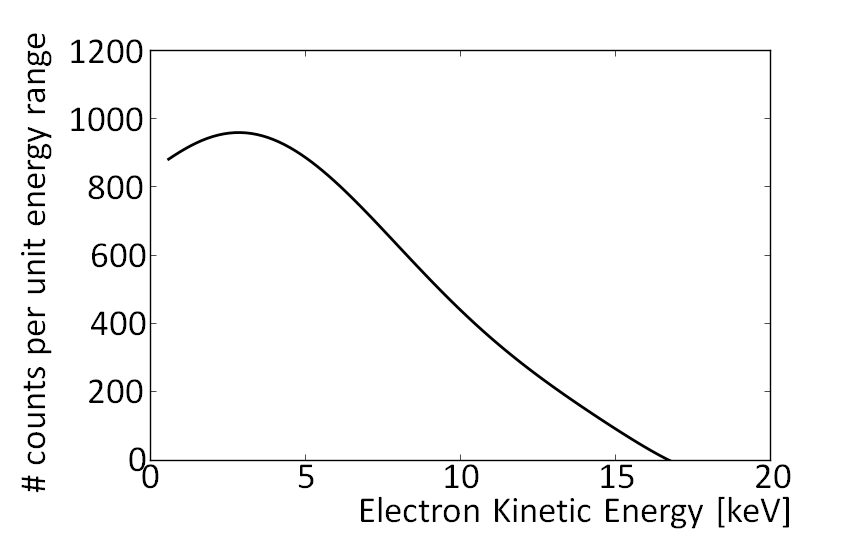
\includegraphics[width=0.7\linewidth]{Chapter1/Figs/Raster/betaSpectrum.png}
 \captionof{figure}[Beta decay spectrum showing electron kinetic energy.]{Beta spectrum reproduced from \cite{griffiths2008neutrino1.5} originally from \cite{lewis1970neutrinos}. The energy of the electron from beta decay varies significantly suggesting a 3 body decay model for beta decay instead of a 2 body model.} %~can be used as a kind of place holder in latex
 \label{fig:beta_spectrum}
\end{figure}

The beta spectrum shown in figure \ref{fig:beta_spectrum} was the first indirect evidence that neutrinos may exist. However, Pauli waited until Chadwick's discovery of the neutron in 1932 \cite{chadwick1932possible} before publishing in 1934 \cite{lederman1970resource}. The complete picture of a proton-neutron nucleus allowed Enrico Fermi to formulate a comprehensive theory of beta decay which incorporated Pauli's neutrino into beta decay\footnote{a translation of Fermi's work was used \cite{wilson1968fermi}} \cite{lederman1970resource} \cite{Fermi:1934hr}. This more complete picture made sure to differentiate the particles of the nucleus (protons and neutrons) from particles that were not bound to it (electrons and neutrinos) \cite{Fermi:1934hr} \cite{wilson1968fermi}. However, this results in a massless neutrino \cite{lederman1970resource}. The discovery of neutrino oscillations (mentioned later in section \ref{section_neutrino_oscillations}) indicates that neutrinos do have mass, but oscillations were discovered long after this  \cite{griffiths2008neutrino1.5}. The more complete picture as illustrated by equation \ref{semi_modern_beta_decay} by Fermi now integrated the neutrino. The discovery of lepton number and the anti-neutrino had not yet been made and so that quantity is not conserved in equation \ref{semi_modern_beta_decay}. 

\begin{equation}
    n \rightarrow p^+ + e^- + \nu
    \label{semi_modern_beta_decay}
\end{equation}

\section{Direct Measurements}\label{Direct_Measurements_section}
%propossal of cowan and riens using a large liquid scintillator detector: \cite{reines1953proposed}
%\\First detection: \cite{reines1953detection}
%\\distingiusing the neutrino and anti-neutrino \cite{davis1959attempt}
%\\Need to find cloud chamber pictures showing the conservation of momentum  \cite{griffiths2008neutrino1.5} shows them, need to find direct source.  \cite{griffiths2008neutrino1.5} also goes on to explain why this matters.
%\\ \cite{michel1949energy} supposedly does show this, but I'm having trouble getting my hands on it, UoL doesn't have access to nature papers! So will just have to include a picture from  \cite{griffiths2008neutrino1.5} and clarifiy it is from \cite{michel1949energy}.
%\\ There is also the suggestion from cowan early on that anti-neutrinos and neutrinos are differing particles,  \cite{cowan1957test}, however this is by no means certain it is possible that neutrinos and anti-neutrinos are differing spin states of the same particle.
%\\ There is also the early suggestion of neutrinos and anti neutrinos being separated by a certain quantity suggested by \cite{konopinski1953universal} under a universal interaction. They use $\mu$ to suggest that certain reactions are not possible, this would later come to be known as lepton number. \\\\
%Suggestions of differing types of neutrino supposedly come from the Soviet union in 1960 but this has been lost to the iron curtain unfortunately I could not find the paper myself. The earliest reference I found is \cite{pontecorvo1963neutrino} in 1963 talking about how this influences astrophysics. 
%\\The direct measurement of differing types of neutrinos was done by \cite{DanbyG1962PhysRevLett.9.36} in 1962. This was done with a pion beam striking a beryllium target and a 10 ton spark chamber behind the target in order to pick up 37 events of one reaction and not another. They also make reference to kions but seem less certain about those due to experimental limitations. They call this the ``The neutrino flip hypothesis.'' This is a really important paper.\\

Experimental evidence for a neutrino had been observed as early as 1949, in figure \ref{pion_path} it is possible to see the change in direction due to the neutrino: the neutrino itself is neutral and so leaves no track in the emulsion. However, the effect of the neutrino can be seen when the anti-pion decays into a muon and when the muon decays into an electron  \cite{griffiths2008neutrino1.5}. Collisions in the emulsion cannot account for the 90$^\circ$ change in direction as the particles decay. Collisions can only account for low angle scattering but not the abrupt changes in direction  \cite{griffiths2008neutrino1.5}. At the time it was practical to assume that the pion decay shown in equation \ref{pion_nolepNo_decay} and the muon decay shown in equation \ref{muon_nolepNo_decay} both produced the same particle when decaying, the neutrino ($\nu$)  \cite{griffiths2008neutrino1.5}. However, as seen in equations \ref{pion_nolepNo_decay} and \ref{muon_nolepNo_decay}, lepton number and neutrino flavour were not yet known and and so are not present in equations \ref{pion_nolepNo_decay} and \ref{muon_nolepNo_decay}.
\begin{equation}
    \pi^- \rightarrow \mu^- + \nu^-
    \label{pion_nolepNo_decay}
\end{equation}
\begin{equation}
    \mu^- \rightarrow e^- + 2\nu
    \label{muon_nolepNo_decay}
\end{equation}
\\
\begin{figure}[!h]
 \centering
 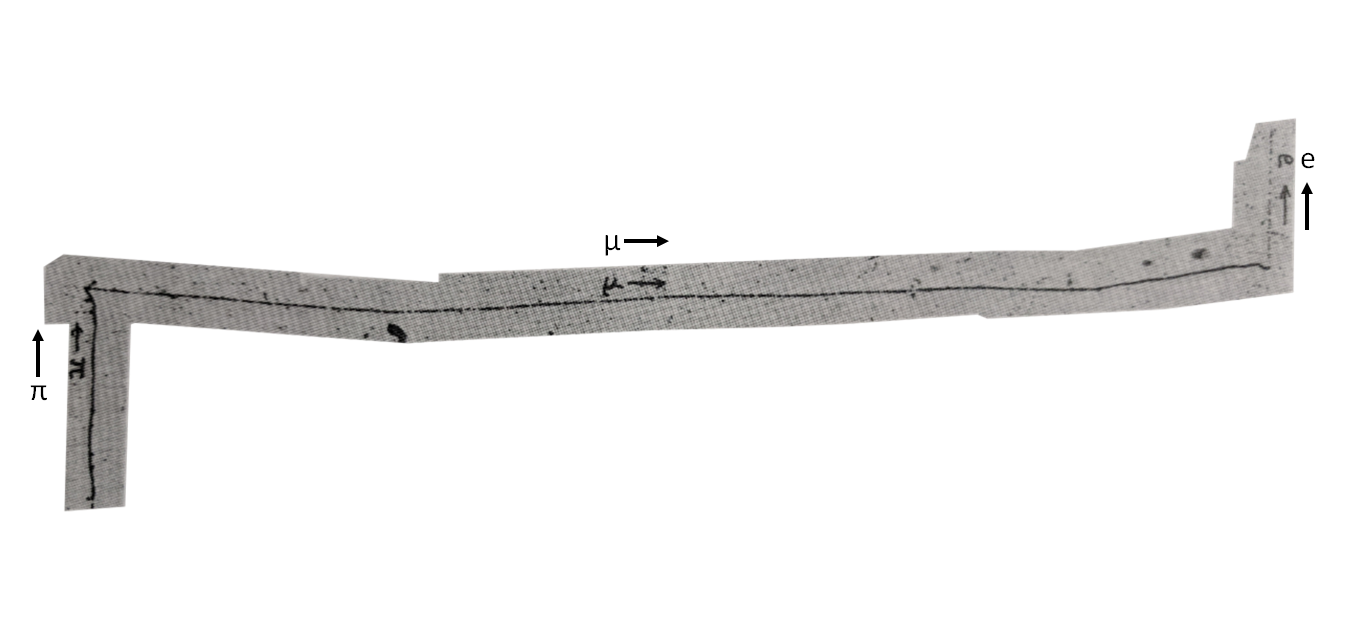
\includegraphics[width=0.8\linewidth]{Chapter1/Figs/Raster/neutrinoInChamberRotated90.png}
 \captionof{figure}[Anti-pion path in emulsion decaying into a muon.]{Path of a anti-pion decaying to a muon emitting one anti-neutrino (equation \ref{pion_nolepNo_decay}) and then that muon decaying into an electron-emitting a neutrino and an anti-neutrino (equation \ref{muon_nolepNo_decay}). The paths at 90$^o$ show particle decay, collisions cannot account for this. From \cite{griffiths2008neutrino1.5} originally published in \cite{michel1949energy}.} %~can be used as a kind of place holder in latex
 \label{pion_path}
\end{figure}
\\The first direct detection of a neutrino would be 22 years after it was proposed in 1931. In 1953, Cowan and Reines proposed a neutrino detector that used a large amount of liquid scintillator to detect neutrinos \cite{reines1953proposed}. Later that same year they constructed a cadmium loaded scintillation detector that used a delayed coincidence measurement of IBD to reduce background \cite{reines1953proposed} \cite{reines1953detection} (result mentioned in section \ref{sec:reactorAntiNeutrinos}). The measurement of neutrino candidates was later reproduced with greater accuracy in 1956 at the Savannah River Plant \cite{Cowan1956Confirmation}. This new detector used a combination of liquid scintillator in three layers and cadmium chloride doped water in another two layers in a ``club-sandwich'' arrangement \cite{Cowan1956Confirmation}. This resulted in an unambiguous measurement of 0.56 $\pm$ 0.06 counts per hour with a signal 20 times higher than the accidental background associated with the reactor \cite{Cowan1956Confirmation}. The delayed coincidence technique assumed $\sim$ 5$\mathrm{\mu}$s between the prompt positron signal and the delayed neutron signal \cite{reines1953detection}. This approach was so successful that its used to this day in many other detector experiments (including the VIDARR detector).
\\\\The difference between neutrinos and anti-neutrinos or their flavours was not yet known. There were two possible hypotheses: Majorana neutrinos where the neutrino and the anti-neutrino are the same particle, and Dirac neutrinos where they are distinct particles  \cite{griffiths2008neutrino1.5} \cite{cowan1957test}. The possibility of Majorana neutrinos was questioned as measurements of double beta decay were found to conflict with the Majorana hypothesis \cite{cowan1957test}. The lifetime of such a particle would be too short compared to measurements made of beta decay \cite{cowan1957test}. A direct attempt at measuring the difference between neutrinos and anti-neutrinos was made in 1959 \cite{davis1959attempt}. The Homestake Mine experiment relied on using $^{37}$Cl and then measuring the amount of $^{37}$Ar produced (equation \ref{neutrino_chlorine_decay}) \cite{davis1959attempt}. From previous experiments the interaction between a neutron and a neutrino (equation \ref{no_lepNo_dirac_nu_capture}) was known to occur \cite{Cowan1956Confirmation}. But whether the anti-neutrino would also act in the same manner (equation \ref{no_lepNo_maj_nu_capture}) was not known. If anti-neutrinos did not act as neutrinos then the Majorana hypothesis was unlikely as neutrinos and anti-neutrinos were probably distinct particles  \cite{griffiths2008neutrino1.5} \cite{davis1959attempt}. Candidates for anti-neutrinos acting as neutrinos (equation \ref{no_lepNo_maj_nu_capture}) were observed 20 times below what would be expected for the Majorana hypothesis \cite{davis1959attempt}. Therefore, Dirac neutrinos were considered to be more consistent with the experiment (though this does not strictly disprove the Majorana hypothesis \cite{griffiths2008neutrino1.5} and searches for neutrino-less double beta decay are ongoing to this day). 
\begin{equation}
    \nu_e + ^{37}Cl \rightarrow  e^- + ^{37}Ar
    \label{neutrino_chlorine_decay}
\end{equation}
\begin{equation}
    n + \nu \rightarrow p^+ + e^-
    \label{no_lepNo_dirac_nu_capture}
\end{equation}
\begin{equation}
    n + \Bar{\nu} \rightarrow p^+ + e^-
    \label{no_lepNo_maj_nu_capture}
\end{equation}
\\This experimental result had been predicted years prior by \cite{konopinski1953universal} which proposed a ``universal interaction'' for ``light'' and ``heavy'' particles. An undetermined phase factor c was represented as $c_P=c_N=c_H$ and $c_e=c_\mu=c_\nu=c_L$ where L and H stand ``light'' and ``heavy'' respectively. In addition to this the muon decays were suggested to give out two differing types of neutrino (equation \ref{noLep_dirac_mu_decay})  \cite{griffiths2008neutrino1.5}, \cite{konopinski1953universal}. Both of these observations would later be consolidated into a quantity known as lepton number with $L=+1$ for electrons, muons and neutrinos but $L=-1$ for positrons, anti-muons and anti-neutrinos \cite{griffiths2008neutrino1.5}. 
\begin{equation}
    \mu^- \rightarrow e^- + \nu + \Bar{\nu}
    \label{noLep_dirac_mu_decay}
\end{equation}
\\However, the conservation of flavours was not yet known hence the lack of neutrino flavours when describing muon decay (equation \ref{noLep_dirac_mu_decay})  \cite{griffiths2008neutrino1.5}. There were hints that flavour conservation was necessary as muon decay into an electron with no neutrinos (equation \ref{mu_forbiden_decay}) was never observed \cite{griffiths2008neutrino1.5}. When a muon decays into an electron two neutrinos must be emitted (equation \ref{noLep_dirac_mu_decay}). The sharp 90$^\circ$ changes in direction with no other particles visible in the emulsion seen in figure \ref{pion_path} strongly suggest neutrino emission. This led to the suggestion that the neutrinos emitted by the decay of muon into electrons were of different types i.e. neutrinos are not anti-neutrinos \cite{Lee:1960tja}  \cite{griffiths2008neutrino1.5}. Thus, redefining lepton numbers to include flavours such that: $L_{e^-} = +1$, $L_{e^+} = -1$, $L_{\mu^-} = +1 $, $L_{\mu^+} = -1 $. With this understanding, equation \ref{noLep_dirac_mu_decay} became equation \ref{proper_mu_decay}.
\begin{equation}
    \mu^- \not\to e^- + \gamma
    \label{mu_forbiden_decay}
\end{equation}
\begin{equation}
    \mu^- \rightarrow e^- + \nu_\mu + \Bar{\nu}_e
    \label{proper_mu_decay}
\end{equation}
\\An experiment to measure the different types of neutrinos was then performed in 1962 \cite{DanbyG1962PhysRevLett.9.36}. This experiment used a pion beam striking a beryllium target and ten 1-ton spark chambers to measure the results. If electron anti-neutrinos and muon anti-neutrinos are the same particle then the production of electrons (equation \ref{test_e_decay}) and the production of muons (equation \ref{test_mu_decay}) should occur at equal rates \cite{DanbyG1962PhysRevLett.9.36}:
\begin{equation}
    \begin{split}
    \nu + n \rightarrow p + e^- \\
    \Bar{\nu} + p \rightarrow n + e^+
    \label{test_e_decay}
    \end{split}
\end{equation}
\begin{equation}
    \begin{split}
    \nu + n \rightarrow p + \mu^-  \\
    \Bar{\nu} + p \rightarrow n + \mu^+
    \label{test_mu_decay}
    \end{split}
\end{equation}
The neutrino ``beam'' used produced 34 muons in the spark chambers 5 of which were considered to be background due to cosmic rays. Therefore $\sim$ 29 electron events were expected to be produced if electron neutrinos and muon neutrinos were the same particle however only 6 candidates were identified \cite{DanbyG1962PhysRevLett.9.36}. To further prove that they were not the same particle two of the 1-ton spark chambers were tested at the electron beams at the Cosmotron, a GeV scale synchrotron, which did produce electrons similar to what would have been expected if they were the same particle. The events from the Cosmotron data set looked very different from the 6 candidate reactions observed from the pion beam being described as ``showers of qualitatively different appearance'' by Danby et. al. \cite{DanbyG1962PhysRevLett.9.36}. The interpretation that electron anti-neutrinos were not muon anti-neutrinos was the most likely conclusion, meaning that there were at least two different flavours of neutrinos \cite{DanbyG1962PhysRevLett.9.36}. And with this information, the modern form of beta decay is shown by equation \ref{modern_beta_decay}.
\begin{equation}
    n \rightarrow p + e^- + \Bar{\nu_e} 
    \label{modern_beta_decay}
\end{equation}

\section{Experimental Evidence For Neutrino Oscillation}\label{sec:neutrinoFlavours}
In the Standard Model it is easier for the neutrino to be assumed as massless, though there is no fundamental reason for neutrinos to be massless, it simplifies much in the standard model if this is the case \cite{griffiths2008neutrinoOscillations}. However, this assumption though simple and neat is now known to be wrong. In particular, the phenomena of neutrino oscillation where neutrinos oscillate between different mass and flavour states proves that neutrinos cannot be massless \cite{griffiths2008neutrinoOscillations}. The first experimental evidence of neutrino oscillations was the solar neutrino problem where the predicted rate by the Standard Solar Model (SSM) by Bahcall in 1968 did not match the measured rate from the previously mentioned Homestake Mine experiment \cite{griffiths2008neutrinoOscillations}. Bahcall attempted to model the expected neutrino rate for the $^{37}$Cl the predicted rate was $3.5 \times 10 ^{-35} \ \textrm{sec}^{-1} \ \textrm{per} \ ^{37}\textrm{Cl} \ \textrm{atom}$ \cite{bahcall1968present}. This conflicted with the measured result from the Homestake Mine of 2.0 $\pm$ 1.2 $\times$ 10 $^{-35}$ sec$^{-1}$ per $^{37}$Cl atom \cite{davis1968homestake}. At the time the large uncertainty on each of these predictions provided some possibility of reconciliation. 
\\\\However, as the Homestake experiment continued to take measurements a discrepancy of about one third became more pronounced over time \cite{griffiths2008neutrinoOscillations}. The Homestake experiment continued to take data until 1995 and produced the result $\Phi$Cl = 2.56 $\pm$ 0.16 Solar Neutrino Unit (SNU) \cite{Bellerive:2003rj}. The SSM continued to be improved and the predicted rate for $\Phi$Cl was 7.6$^{+ 1.3}_{-1.1}$ SNU \cite{Bellerive:2003rj} \hl{talk about what a solar neutrino unit is}. But chlorine is not the only way in which neutrinos can be measured. The Sudbury Neutrino Observatory (SNO) used heavy water to measure neutrino interaction and the Kamiokande and later Super-Kamiokande (SuperK) experiments would use normal water to measure neutrino interactions \cite{Bellerive:2003rj}. These experiments are sensitive to different parts of the solar neutrino spectrum with SuperK and SNO being more sensitive to higher energies than the chlorine experiments \cite{Bellerive:2003rj}. The SuperK experiment used neutrino scattering to detect any type of neutrino but is 6.5 times more sensitive to electron neutrinos \cite{griffiths2008neutrinoOscillations}. SNO also works through neutrino scattering but also works through the charged-current (CC) interaction and  the neutral-current (NC) interaction) \cite{sno2001}\cite{Bellerive:2003rj} \cite{griffiths2008neutrinoOscillations}. 
\\\\By combining the results from SuperK which uses exclusively neutrino scattering and the SNO results for CC it is possible to solve the solar neutrino problem. SuperK found 45.1\,\% $\pm$ 0.5\,\% (stat)$^{+1.6\,\%}_{-1.4\,\%}$ (syst) according to the BP2000 standard solar model \cite{superK2001}. Whereas the CC interaction results from SNO found 34.7\,\% $\pm$ 2.9\,\% of the expected electron neutrino flux\cite{sno2001}. There is a $\sim$ 10\,\% discrepancy between these two results. But this does not mean 10\,\% of the neutrinos were muon neutrinos and tau neutrinos, as the SuperK detector is 6.5 times more sensitive to electron neutrinos. 10\,\% $\times$ 6.5 = 65\,\%, therefore 65\,\% of the neutrinos are muon and tau flavoured neutrinos. And so all neutrinos are now accounted for as the Cl results from SNO accounted for the other 35\,\% and thus the solar neutrino problem was deemed solved  \cite{griffiths2008neutrinoOscillations}. The results showed that neutrino oscillations had a clear experimental basis for their existence proving that the solar neutrinos were changing flavours as they traversed through space. 
\\\\In addition, atmospheric neutrino oscillation has also been observed. Atmospheric neutrino production is dominated by production from equations \ref{equ:pi+AtmosNu} and \ref{equ:mu+AtmosNu} (and their charge conjugates):
\begin{equation}
    \pi^+ \rightarrow \mu^+ + \nu_\mu
    \label{equ:pi+AtmosNu}
\end{equation}
\begin{equation}
    \mu^+ \rightarrow e^+ + \Bar{\nu_\mu} + \nu_e
    \label{equ:mu+AtmosNu}
\end{equation}
This gives an expected ratio of muon neutrinos and muon anti-neutrinos to electron neutrinos and electron anti-neutrinos of $\sim$ 2 (equation \ref{equ:ratioAtmosNu}) \cite{fukuda_skAtmosAnnounce_1998}:
\begin{equation}
    R_{\textrm{data}/\textrm{MC}} = (N_\mu/N_e)_{\textrm{data}}/(N_\mu/N_e)_{\textrm{MC}} \approx 2
    \label{equ:ratioAtmosNu}
\end{equation}
But instead more equal numbers were found \cite{fukuda_skAtmosAnnounce_1998} \cite{KAJITA_sk_atmospheric_2016}. Atmospheric neutrino disappearance was found in the IMB detector in 1986 \cite{tjHaines_AtmosModel_1986} and was also observed in SuperK in 1988 \cite{Hirata_sk_atmosStudy_1988} \cite{KAJITA_sk_atmospheric_2016}. By 1986 and 1988 the theory of oscillations was quite well known and this was suggested in 1986 as a possible explanation \cite{tjHaines_AtmosModel_1986}. But it took until 1998 when SuperK calculated an R$_{\textrm{data}/\textrm{MC}}$ value of $\approx = 0.63 - 0.65$, depending on energy range \cite{fukuda_skAtmosAnnounce_1998}. 
\\\\These results show how the theory of neutrino oscillations has strong experimental backing. This is important as the simplest scenario of massless neutrinos cannot explain the results of atmospheric and solar neutrino disappearance and reappearance that oscillations can. And as such this subsequent rejection of massless neutrinos and strong favouring of neutrino oscillations highlights why the theory of oscillations needs to be considered for any neutrino experiment. 

% \section{Solar Neutrinos}
% %This section will mainly be on the solar neutrino problem and how it was solved. The main players here are the homestake %experiment for detecting a certain number of neutrinos  \cite{davis1968homestake}. Bahcall for predicting three times more %solar neutrinos than were detected from that experiment \cite{bahcall1968present}. As well as the Kamiokande-II experiment %which made measurements in 1989 \cite{Kamiokande-II1989} which predicted $\sim$ 0.46 times the predicted $\nu$ flux from %the sun. And then finally the SNO and superK experiments in 2001 which are considered the final confirmation. SuperK %reference being \cite{superK2001}. And \cite{sno2001} for SNO.
% %\\This section may also be well served by explaining the proton-proton chain briefly as well as mentioning the CNO cycle %that isn't the power mechanism for our sun, if only because the 1968 papers mention it. Also figure out how to do sub %references for  \cite{griffiths2008neutrinoOscillations}. 
% %\\ \cite{Bellerive:2003rj} presents some good plots and a nice overview of the neutrino experiments that lead up to the %discovery of the neutrino oscillations. A nice overview.
% Whilst the neutrino flavous were being confirmed \cite{DanbyG1962PhysRevLett.9.36} preperations to measure the solar neutrino flux were also underway. The first measurement in the Homestake mine in 1968 found 31 $\pm$ 10 neutrinos from the sun \cite{davis1968homestake} by using $^{37}$Cl which interacts with $\nu_e$ as shown in equation \ref{neutrino_chlorine_decay} \cite{Bellerive:2003rj}. Which measured the production of $\nu_e$ from $^8$B interactions in the sun ($^8$B neutrino production is preferred due to the higher energy of neutrinos produced \cite{griffiths2008neutrinoOscillations}). Originally, this measurement was attempting to conclude whether the CNO cycle played a significant role in the sun's power production, concluding that it was less than 9\% of the power produced \cite{davis1968homestake}. However, when Bahcall attempted to model the expected neutrino rate for the $^{37}$Cl the predicted rate was 3.5 $\times$ 10 $^{-35}$ sec$^{-1}$ per $^{37}$Cl atom. Which conflicted with the measured result from the Homestake mine of 2.0 $\pm$ 1.2 $\times$ 10 $^{-35}$ sec$^{-1}$ per $^{37}$Cl atom \cite{davis1968homestake}. This is considered to be the birth of the solar neutrino problem \cite{griffiths2008neutrinoOscillations}. But it is worth pointing out this is somewhat of a retroactive view. At the time it was hoped that these discrepancies would be resolved as the errors were significant. In fact the prediction paper concluded ``...there is no irreconcilable discrepancy between our predictions and the experiment of Davis, Harmer, and Hoffman when the uncertainties in the various parameters that enter the calculation are taken into account'' \cite{bahcall1968present}.
% \\\\However, as the Homestake experiment continued to run a discrepancy of $\sim 1/3$ became more pronounced over time \cite{griffiths2008neutrinoOscillations}. The Homestake experiment continued to take data until 1995 and produced the result $\Phi$Cl = 2.56 $\pm$ 0.16 Solar Neutrino Unit (SNU) \cite{Bellerive:2003rj}. The standard solar model (SSM) continued to be improved and the predicted rate for $\Phi$Cl was 7.6$^{+ 1.3}_{-1.1}$ SNU \cite{Bellerive:2003rj}. However, chlorine is not the only way in which neutrinos can be measured the Sudbury Neutrino Observatory (SNO) used heavy water to measure neutrino interaction and the Kamiokande and later SuperKamiokande (SuperK) experiments would use normal water to measure neutrino interactions \cite{Bellerive:2003rj}. These experiments are sensitive to different parts of the solar neutrino spectrum as seen in figure \ref{neutrino_emmision_graph} with SuperK and SNO being more sensitive to higher energies than the chlorine experiments. The SuperK experiment used neutrino scattering (equation \ref{neutrino_scattering}) to detect any type of neutrino but is 6.5 times more sensitive to electron neutrinos  \cite{griffiths2008neutrinoOscillations}. SNO also works through neutrino scattering but also works through the charged-current (CC) reaction (equation \ref{charged-current_reaction}) and  the neutral-current (NC) reaction (equation \ref{neutral-current_reaction}) \cite{sno2001}\cite{Bellerive:2003rj}  \cite{griffiths2008neutrinoOscillations}. 
% \begin{figure}[!h]
%  \centering
%  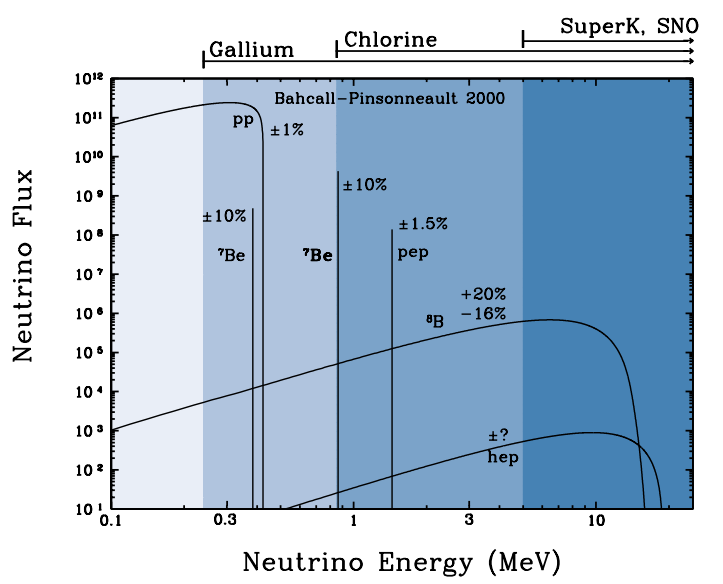
\includegraphics[width=0.7\linewidth]{Chapter1/Figs/Raster/neutrino_emmision_graph.png}
%  \captionof{figure}{The solar neutrino spectra predicted by the SSM. From \cite{Bellerive:2003rj}. The neutrino fluxes at one astronomical unit from continuum sources are given in units of cm$^{-2}$ s$^{-1}$ MeV$^{-1}$ , and the line fluxes are given in cm$^{-2}$ s$^{-1}$.} %~can be used as a kind of place holder in latex
%  \label{neutrino_emmision_graph}
% \end{figure}
% \begin{equation}
%     \nu + e \rightarrow  \nu + e
%     \label{neutrino_scattering}
% \end{equation}
% \begin{equation}
%     \nu_e + d \rightarrow p + p + e 
%     \label{charged-current_reaction}
% \end{equation}
% \begin{equation}
%     \nu + d \rightarrow  n + p + \nu
%     \label{neutral-current_reaction}
% \end{equation}
% \\By combining the results from SuperK which uses exclusively neutrino scattering and the SNO results for CC it is possible to solve the solar neutrino problem. SuperK found 45.1\,\% $\pm$ 0.5\,\% (stat)$^{+1.6\,\%}_{-1.4\,\%}$ (syst) according to the BP2000 standard solar model \cite{superK2001}. Whereas the CC results from SNO found 34.7\,\% $\pm$ 2.9\,\% of the $\nu_e$ expected as seen in figure \ref{sno_superK_comparision_plot} \cite{sno2001}. There is a $\sim$ 10\,\% discrepancy between these two results. But this does not mean 10\,\% of the neutrinos were $\nu_\mu$ and $\nu_\tau$, as the SuperK detector is 6.5 times more sensitive to $\nu_e$. 10\,\% $\times$ 6.5 = 65\,\%, therefore 65\,\% of the neutrinos are $\nu_\mu$ and $\nu_\tau$. And so all neutrinos are now accounted for as the Cl results from SNO accounted for the other 35\,\% and thus the solar neutrino problem was deemed solved  \cite{griffiths2008neutrinoOscillations}. The result was that neutrino oscillations had a clear experimental basis for their existence. As it was clear that the solar neutrinos were changing flavours as they traversed through space. 

% %\cite{Ashenfelter:2015tpm} %prospect citation

% \begin{figure}[!h]
%  \centering
%  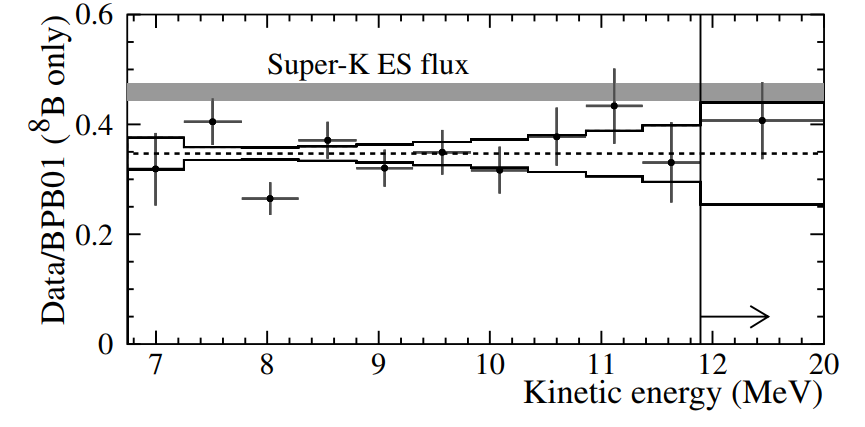
\includegraphics[width=0.7\linewidth]{Chapter1/Figs/Raster/superKSnoComparison.png} %height of this plot had to be adjusted because of its unusal diemensions
%  \captionof{figure}{The ratio of the data to the expected kinetic energy distribution with correlated systematic errors for the $^8$B charged current interactions. Notice the $\sim$ 10 \,\% discrepancy in data between the super K elastic scattering flux (in shaded grey) and the SNO charged current flux (the dashed line). From \cite{sno2001}.} %~can be used as a kind of place holder in latex
%  \label{sno_superK_comparision_plot}
% \end{figure}


% %\begin{figure}[!h]
% % \centering
% % 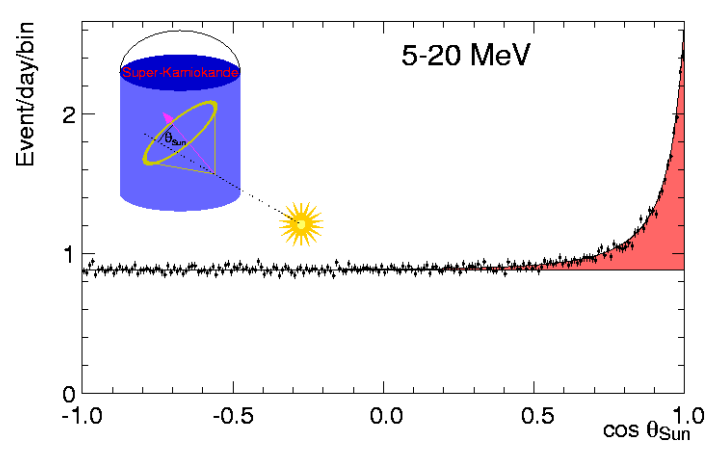
\includegraphics[height=90mm]{sk_angular_neutrinos.png}
% % \captionof{figure}{from \cite{Bellerive:2003rj}} %~can be used as a kind of place holder in latex
% % \label{sk_angular_neutrinos}
% %\end{figure}

\section{Two Neutrino Oscillation Theory} \label{section_neutrino_oscillations}
% Neutrino oscillations were proposed in 1968 after the Davis experiment \cite{davis1968homestake}. A man called Pontecorvo discussed the possibility of oscillations in 1957 and revived the idea in 1968 as a solution to the solar neutrino problem \cite{griffiths2008neutrinoOscillations}. With the original 1958 paper being \cite{pontecorvo1958_OscillationProposal}, suggesting the transformation of Kiaons. And the suggestion for the solution to the solar neutrino problem being here \cite{pontecorvo_gibov_1969_solar_oscillation}. Note these are a little hard to get hold of but some old russian servers still have them, Googling not too hard. 
% \\Most of this section will follow  \cite{griffiths2008neutrinoOscillations}. There is a more in depth explanation using \cite{sassaroli1999neutrino} in which  \cite{griffiths2008neutrinoOscillations} follows the standard treatment for neutrino oscillations. \cite{sassaroli1999neutrino} also goes through a relativistic treatment but that's probably too much for this overview and not really necessary for explaining the phenomena of oscillations, it should still be mentioned though. Wavelength of neutrino and kaon oscillations mentioned before are outlined by \cite{burkhardt2003wavelength}, it goes through the kinematics and shows that the oscillations do account for the mass difference, again quite in depth maybe overkill... should talk to one of my supervisors about this... 
% \\Also there is the MSW (named after the people who found it) effect however the exact papers appear to be a bit difficult to find but I was able to get something very detailed from Mikheev 1987 which goes into interactions with matter \cite{Mikheev_1987}.
Neutrino oscillations had been proposed in 1958 by Pontecorvo by analogy with neutral kaons and neutral anti-kaons   \cite{griffiths2008neutrinoOscillations} \cite{pontecorvo1958_OscillationProposal}. This approach was later revived when as a solution to the solar neutrino problem in 1969 \cite{pontecorvo_gibov_1969_solar_oscillation}. When the Davis and Harmer experiment in 1968 failed to produce the number of expected neutrinos in comparison to the SSM the idea of neutrino oscillations was revisited to explain this discrepancy \cite{pontecorvo_gibov_1969_solar_oscillation}. At the time, the reactor based neutrino experiments excluded an oscillation length smaller than a few metres but to measure the true oscillation length would require measuring the neutrino production from the sun. This was due to the lengths involved ($\mathcal{O} \sim$ 10$^6$\,km) \cite{pontecorvo_gibov_1969_solar_oscillation} and as seen in table \ref{solar_nuetrino_table} the mechanisms for solar neutrinos all produce electron neutrinos so if any oscillations occur a discrepancy would be visible. 

\begin{table*}[!h]
\centering
\begin{tabular}{lllll}  
\toprule
\multicolumn{1}{c}{Reaction} & \multicolumn{1}{c}{Label} & \multicolumn{1}{c}{Flux [cm$^{-2}$s$^{-1}$]}
\\
\cmidrule(r){1-1}
\cmidrule(r){2-2}
\cmidrule(r){3-3}
p+p $\rightarrow$ $^2$H+e$^+$+$\nu_e$           & pp                & 5.95 $\times$ 10$^{10}$\\
p+e$^-$+p$\rightarrow$ $^2$H+ $\nu_e$           & pep               & 1.40 $\times$ 10$^{8}$\\
$^3$He+p $\rightarrow$ $^4$He+e$^+$+ $\nu_e$    & hep               & 9.3  $\times$ 10$^{3}$\\
$^7$Be+e$^-$ $\rightarrow$ $^7$Li+ $\nu_e$      & $^7$Be            & 4.77 $\times$ 10$^{9}$\\
$^8$B $\rightarrow$ $^8$Be$^*$+e$^+$+ $\nu_e$   & $^8$B             & 5.05 $\times$ 10$^{6}$\\
\bottomrule   
\end{tabular}
\caption{Neutrino production from fusion reactions in the Sun from \cite{Bellerive:2003rj} }
\label{solar_nuetrino_table}
\end{table*}

%Then there is the full quantum mechanical treatment of neutrino oscillations which uses ``Diagonalization of the two coupled Dirac equations'' and ``Field quantization, anticommutation relations and flavour wave functions'' \cite{sassaroli1999neutrino}

In order to predict the number of neutrinos oscillating between one state and another, there are two approaches that can be taken. The approach that will be taken is to treat the two systems as a linear combination of eigenstates electron neutrinos and muon neutrinos which is considered the ``standard treatment'' \cite{sassaroli1999neutrino}  \cite{griffiths2008neutrinoOscillations}.
\\\\Begin with two eigenstates, 1 and 2: 
\begin{equation}
    \begin{bmatrix}
        \ket{\nu_1} \\
        \ket{\nu_2}
    \end{bmatrix}
    =
    \begin{bmatrix}
        \cos\theta & -\sin\theta \\
        \sin\theta & \cos\theta 
    \end{bmatrix}
        \begin{bmatrix}
        \ket{\nu_e} \\
        \ket{\nu_\mu}
    \end{bmatrix}
    \label{linear_combination_eq_1}
\end{equation}
We then introduce the amplitudes for detecting an electron neutrino ($C_e$) and a for detecting a muon neutrino ($C_\mu$). Then the two amplitudes ($C_1$, $C_2$) for the neutrino energy states ($E_1$, $E_2$) are introduced. These two amplitudes evolve over time as:
%Then introduce $C_1$ and $C_2$ which are the amplitudes for finding the neutrino in the energy states $E_1$ and $E_2$ , respectively. The coefficients $C_1$ and $C_2$ evolve over time as:
\begin{equation}
    C_1(t) = C_1(0)e^{-iE_1t}, \quad  C_2(t) = C_2(0)e^{-iE_2t}
    \label{linear_combination_eq_1.5}
\end{equation}
Which is known from the Schrödinger equation \cite{sassaroli1999neutrino} \cite{griffiths2008neutrinoOscillations}. We then introduce the rotation matrix between the flavour and mass eigenstates (equation \ref{linear_combination_eq_1}) yielding the following relation between the energy and flavour amplitude:
\begin{equation}
    \begin{bmatrix}
        C_1(t) \\
        C_2(t)
    \end{bmatrix}
    =
    \begin{bmatrix}
        \cos\theta & -\sin\theta \\
        \sin\theta & \cos\theta 
    \end{bmatrix}
        \begin{bmatrix}
        C_e(t) \\
        C_\mu(t)
    \end{bmatrix}
    \label{linear_combination_eq_2}
\end{equation}
By then multiplying by the inverse of the sine cosine matrix and substituting in using equation \ref{linear_combination_eq_1.5} the following relation follows:
\begin{equation}
    \begin{bmatrix}
        C_e(t) \\
        C_\mu(t)
    \end{bmatrix}
    =
    \begin{bmatrix}
        \cos\theta & -\sin\theta \\
        \sin\theta & \cos\theta 
    \end{bmatrix}
        \begin{bmatrix}
        C_1(0)e^{-iE_1t} \\
        C_2(0)e^{-iE_2t}
    \end{bmatrix}
    \label{linear_combination_eq_3}
\end{equation}
A boundary condition is imposed corresponding to the neutrino flavour at the time of production. At time of 0 a muon neutrino is produced and this corresponds to:
\begin{equation}
    C_\mu(0) = 1, \quad C_e(0) = 0
    \label{linear_combination_eq_4}
\end{equation}
By inserting these values into equation \ref{linear_combination_eq_2} the following is obtained:
\begin{equation}
    C_1(0) = -\sin\theta, \quad C_2(0) = \cos\theta
    \label{linear_combination_eq_5}
\end{equation}
In order to get the time evolution of the flavour amplitudes, equation \ref{linear_combination_eq_5} is substituted into equation \ref{linear_combination_eq_3} to receive the following relations for electron and muon neutrinos: 
\begin{equation}
    C_e(t)=\sin\theta\cos\theta(e^{-iE_2t}-e^{-iE_1t})
    \label{linear_combination_eq_6}
\end{equation}
\begin{equation}
    C_\mu(t)=\sin^{2}e^{-iE_1t} + \cos^{2}e^{-iE_2t}
    \label{linear_combination_eq_7}
\end{equation}
%side note what is l I think griffiths talks about it...
Space and therefore momentum are then introduced by assuming in equations \ref{linear_combination_eq_6}, \ref{linear_combination_eq_7}: 
\begin{equation}
   E_1^2=m_1^2 + p^2, \quad E_2^2=m_2^2  , \quad L \approx t
    \label{linear_combination_eq_8}
\end{equation}
(Note that L $\approx ct$ but in the following $c$ is assumed to be 1 i.e natural units are used). 
\\Thus, the probability for the neutrino flavour oscillations between muon and electron neutrinos is as follows: 
\begin{equation}
   {\mid{C_e}\mid}^2 = \sin^2(2\theta)\sin^2[(E_2-E_1)t/2] \approx \sin^2(2\theta)\sin^2\left[\frac{(m_1^2-m_2^2)L}{4E}\right]
    \label{linear_combination_eq_9}
\end{equation}
\begin{equation}
    {\mid{C_\mu}\mid}^2 = 1 - \sin^2(2\theta)\sin^2[(E_2-E_1)t/2] \approx 1 - \sin^2(2\theta)\sin^2\left[\frac{(m_1^2-m_2^2)L}{4E}\right]
    \label{linear_combination_eq_10}
\end{equation}
Note that for equation \ref{linear_combination_eq_9} and equation \ref{linear_combination_eq_10} that energy equals momentum, these equations also have to be averaged over the energy distribution of particles involved. Also, the assumption that the muon neutrino is created with a definite momentum is only an approximation \cite{sassaroli1999neutrino}. This explanation follows \cite{sassaroli1999neutrino} which also gives the full quantum mechanical treatment as well. In equation \ref{linear_combination_eq_9} a distance dependant term ($L$) is now present, specifically at equation \ref{equ:maxConversionToElectronNeutrinos}: 
\begin{equation}
    L = (4E\pi) / (m_1^2 - m_2^2)
    \label{equ:maxConversionToElectronNeutrinos}
\end{equation}
there will be a maximum conversion to electron neutrinos and at twice the length in equation \ref{equ:maxConversionToElectronNeutrinos} there will be a maximum conversion to muon neutrinos, the oscillations vary with distance and energy. When converting from natural units to MeV/m the equations \ref{equ:peToPmu} and \ref{equ:pmuToPe} are produced (conversion from natural units to MeV/m taken from \cite{steveBoydLectureNotes}). Then values from equation \ref{equ:sinSqTheta21}: 
\begin{equation}
\sin^2(\theta_{12}) = 0.307\hspace{1cm} \Delta m^2_{21} = 7.53 \times 10^{-5}\,\textrm{eV}^2
\label{equ:sinSqTheta21}
\end{equation}
are taken from the PDG \cite{Zyla_pdg_2020} so that a graph of oscillation probabilities can be created. When modelling energies in figure \ref{fig:probabilityNeutrinoTransition} for reactor monitoring a detector needs to be placed at $\sim$~1000\,m to measure standard neutrino oscillations. This is in line with the distance required for Double Chooz to see neutrino disappearance in the far detector (a distance of 1050\,m) \cite{lasserre2006} \cite{Abe_2012} \cite{abe2014improved}. In figure \ref{fig:probabilityNeutrinoTransition} it is assumed that the minimum detectable neutrino energy from a reactor is 1.8\,MeV and the maximum is 8.5\,MeV and the range for near-field varies between 10\,m -- 100\,m. The highlighted area in figure \ref{fig:probabilityNeutrinoTransition} shows that for near-field reactor monitoring standard neutrino oscillations should not be a concern and so are not a concern for VIDARR a detector placed. \hl{I have a note here to look through boyds lecture notes and talk about the mass eigenstates and how they interact through the weak eigenstates}

\begin{equation}
    P(\nu_e \rightarrow \nu_\mu) = \sin^2(2\theta)\sin^2\left[1.27\frac{({\Delta m_{21}}^2)L}{E}\right]
    \label{equ:peToPmu}
\end{equation}
\begin{equation}
    P(\nu_\mu \rightarrow \nu_e) = 1 -  \sin^2(2\theta)\sin^2\left[1.27\frac{({\Delta m_{21}}^2)L}{E}\right]
    \label{equ:pmuToPe}
\end{equation}

\begin{figure}[!h]
  \centering
  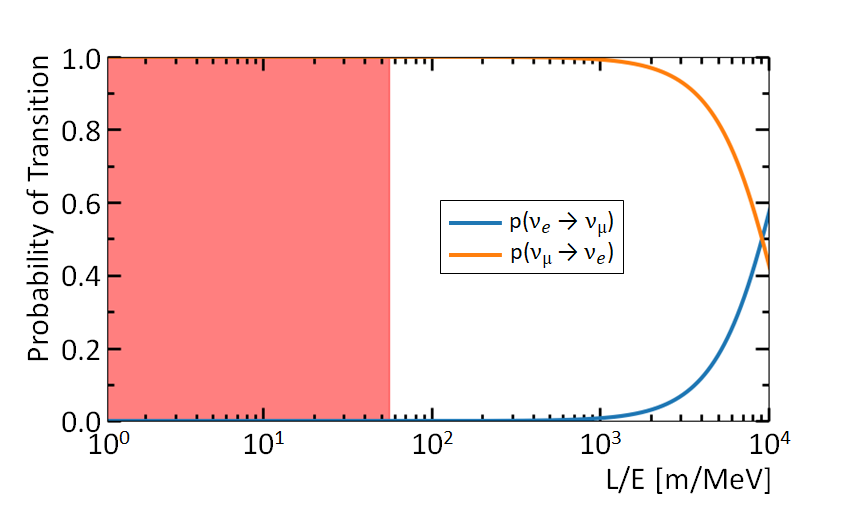
\includegraphics[width=0.8\linewidth]{Chapter2/Figs/neutrinoLOverE_0-2000_ReactorRanges_10-8.5_100-1.8_Log_Adjusted_MedText.png}
  \captionof{figure}[L/E values for the two neutrino case.]{L/E values for the two neutrino case. Assuming near-field ranges between 10\,m -- 100\,m and reactor anti-neutrino energies of 1.8\,MeV -- 8.5\,MeV \cite{Mueller_2011} L/E values of 1.18\,m/MeV -- 55.6\,m/MeV are produced and shown via the highlighted area. In the highlighted area there is no significant probability of standard neutrino oscillation.}%The L/E values for neutrino transition for a two neutrino case. The highlighted area represents reactor neutrinos assuming a minimum detectable neutrino energy of 1.8\,MeV and maximum of 8.5\,MeV for reactors \cite{Mueller_2011}. Near-field reactor monitoring distances are assumed to vary between 10\,m to 100\,m. This leads to a minimum L/E of 10\,m/8.5\,MeV = 1.18\,m/MeV and a maximum L/E of 100\,m/1.8\,MeV = 55.6\,m/MeV. The expected range for neutrino oscillation is significantly above the reactor monitoring range and as such typical neutrino oscillations will not be a significant effect for near-field reactor monitoring between 10\,m -- 100\,m.}
\label{fig:probabilityNeutrinoTransition}
\end{figure}

%white space
%\vspace{5cm}

\section{Mixing Angles}
% Firstly it would be a good idea to pull from \cite{griffiths2008neutrinoOscillations} which does mention that according to equations \ref{linear_combination_eq_9} and \ref{linear_combination_eq_9} the masses must be unequal and cannot be zero. i.e. $m_i \neq m_j$ and $\Delta m_\theta \neq 0$. \\
% The review of particle physics 2014 is probably quite useful here\cite{Olive_2014}, this may also start to bleed into the other sections, results from T2K, dayabay, double CHOOZ and KamLand may need to be added here. As this is quite a difficult section, lot of potential pit falls and I need to make sure the info I give is up to date because the information is changing frequently. 
% \\I need to show the neutrino mixing matrix and how the dirac and Majorana components work with the mixing angles as shown below (the PMNS matrix) 
% \begin{equation}
% U
%     =
%     \begin{bmatrix}
%         c_{12}c_{13} & s_{12}c_{13} & s_{13}e^{-i\delta}\\
%         -s_{12}c_{23} - c_{12}s_{23}s_{13}e^{i\delta} & c_{12}c_{23} - s_{12}s_{23}s_{13}e^{i\delta} & s_{23}c_{13} \\
%         s_{12}s_{23} - c_{12}c_{23}s_{13}e^{i\delta} & -c_{12}s_{23} - s_{12}c_{23}s_{13}e^{i\delta} & c_{23}c_{13} 
%     \end{bmatrix}
%     \\ \times \text{diag}(1, e^{\frac{i\alpha21}{2}} , e^{\frac{i\alpha31}{2}})
%     \label{neutrino_mixing_matrix}
% \end{equation}
% The dirac CP violation phases are represented by the $\delta$ components the Majorana CP violation is represented by the $\alpha$ components this was taken from \cite{Olive_2014}, which extrapolated it from \cite{Bilenky_1980}, \cite{Schechter_and_Valle_1980} both of which are heavily cited articles themselves.It may be a good idea to mention the CKM quark mixing matrix too. and also cite it. 
% \\I also need to cite double chooz whilst \cite{Olive_2014} has a good handle on $\theta_{12}$ (solar) and $\theta_{23}$ (atmosphere) the value of $\theta_{13}$ (reactor) was before the latest results of the double chooz experiments. So I need to hunt down there most recent paper of which I found was \cite{abe2014improved}, but that was in 2014... It is also worth pointing out as \cite{Olive_2014} does that the oscillations for neutrinos will be very different to the oscillations that quarks undergo these mixing angles are very different. Also worth pointing out that so far no evidence for Majorana neutrinos has be found. Mention neutrino-less double beta decay as a possibility for Majorana neutrinos or at least an exclusion of dirac neutrinos \cite{Schechter_and_Valle_1982}. latest. 
According to equations \ref{linear_combination_eq_9} -- \ref{equ:pmuToPe} for oscillations to occur there must be mass differences between the two neutrino types. If neutrinos were massless then the oscillations could not occur as the values for the probabilities would be zero according to equations \ref{linear_combination_eq_9} -- \ref{equ:pmuToPe}. Therefore, the existence of neutrino oscillations shows that the assumption of massless neutrinos is incorrect \cite{griffiths2008neutrinoOscillations} \cite{sassaroli1999neutrino}. It is assumed that the neutrino flavours follow lepton flavour giving: electron neutrinos, muon neutrinos, and tau neutrinos. The flavour eigenstates dictate neutrino interactions, but neutrinos propagate as flavour eigenstates of the free-particle Hamiltonian - the mass eigenstates 1, 2 and 3. The flavour mass eigenstates evolve complexly due to the three different masses contributing to the pattern   \cite{griffiths2008neutrinoOscillations}. 
\\\\These flavour changes can be represented by three different angles, the solar angle ($\theta_{12}$), the atmospheric angle ($\theta_{23}$), and the reactor angle ($\theta_{13}$) \cite{Olive_2014}  \cite{griffiths2008neutrinoOscillations}. These angles can be represented by the following  matrix in equation \ref{PMNS_matrix} which is referred to as the Pontecorvo–Maki–Nakagawa–Sakata (PMNS) matrix.
\begin{equation}
U
    =
    \begin{bmatrix}
        c_{12}c_{13} & s_{12}c_{13} & s_{13}e^{-i\delta}\\
        -s_{12}c_{23} - c_{12}s_{23}s_{13}e^{i\delta} & c_{12}c_{23} - s_{12}s_{23}s_{13}e^{i\delta} & s_{23}c_{13} \\
        s_{12}s_{23} - c_{12}c_{23}s_{13}e^{i\delta} & -c_{12}s_{23} - s_{12}c_{23}s_{13}e^{i\delta} & c_{23}c_{13} 
    \end{bmatrix}
    \\ \times \text{diag}(1, e^{\frac{i\alpha21}{2}} , e^{\frac{i\alpha31}{2}})
    \label{PMNS_matrix}
\end{equation}
Where $s_{ij}$ and $c_{ij}$ represent $\sin(\theta_{ij})$ and $\cos(\theta_{ij})$ respectively. The equation is also parameterized by the CP violation phases $\delta$ and $\alpha$ which represent the Dirac and Majorana phases respectively \cite{Olive_2014}. However, at this time experiments to prove the Majorana over Dirac neutrinos have not proven fruitful as neutrino-less double beta decay has not been observed due to the challenging theoretical and experimental requirements (though experiments are improving their precision) \cite{Cardani_2019}.  So the above PNMS matrix is often written without the Majorana component ($\text{diag}(1, e^{\frac{i\alpha21}{2}} , e^{\frac{i\alpha31}{2}})$). 
\\\\Reducing the errors on the mixing angles has been ongoing effort in neutrino physics. As a result, there are many experiments that have contributed to the improvements in angles which can be seen in figure \ref{neutrino_angles_experiments_variations} 
 which shows the regions favoured or excluded by the oscillation experiments. The measurement of solar neutrinos and the resulting solar neutrino problem has already been covered. And due to the abundance of solar neutrinos the solar angle has been measured frequently as seen in figure \ref{neutrino_angles_experiments_variations}. There is also an abundance of terrestrial muon neutrinos which are produced in the atmosphere from cosmic proton interactions which in turn produce pions which decay into muons and muon neutrinos \cite{griffiths2008neutrinoOscillations} (see equations \ref{pi_plus_neutrino_production}, \ref{pi_minus_neutrino_production}).
\begin{equation}
    \pi^+ \rightarrow \mu^+ + \nu_\mu,\quad \mu^+ \rightarrow e^+ + \nu_e + \Bar{\nu}_\mu 
    \label{pi_plus_neutrino_production}
\end{equation}
\begin{equation}
    \pi^- \rightarrow \mu^- + \nu_\mu, \quad \mu^- \rightarrow e^- + \nu_e + \Bar{\nu}_\mu 
    \label{pi_minus_neutrino_production}
\end{equation}
\begin{figure}[!h]
 \centering
 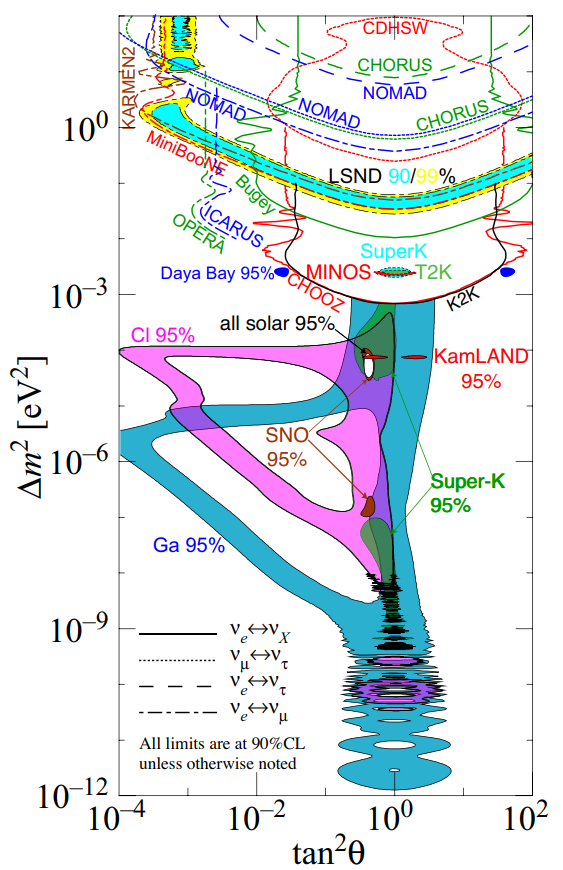
\includegraphics[height=100mm]{Chapter1/Figs/Raster/neutrino_angles_experiments_variations.png} %height of this plot had to be adjusted because of its unusal diemensions
 \captionof{figure}[Regions of squared-mass splitting and mixing angle.]{The regions of squared-mass splitting and mixing angle favoured or excluded by various experiments based on two-flavour neutrino oscillation analyses. From \cite{Olive_2014}.} %~can be used as a kind of place holder in latex
 \label{neutrino_angles_experiments_variations}
\end{figure}
Therefore, there has been an increase in the number of experiments measuring the reactor neutrino angle however due to the production of electron neutrinos from the sun this presents a unique challenge \cite{Olive_2014}. The solution is to use reactor produced electron anti-neutrinos at a baseline of $\sim$ 1\,km such that oscillations driven by the solar mass neutrino difference are negligible. The first experiment to do this was the Chooz experiment, however, it was unable to find any evidence of electron anti-neutrino disappearance \cite{Olive_2014}. But the experiment was revised into the Double Chooz experiment which has been able to measure electron anti-neutrino disappearance (see section  \ref{subSec:doubleChooz}). These results are also corroborated by RENO (see section \ref{subSec:reno}). The current values are $\sin^2(\theta_{12}) = 0.307 \pm 0.013$, $\sin^2(\theta_{23}) = 0.546 \pm 0.021$, and $\sin^2(\theta_{13}) = 0.0220 \pm 0.0007$ according to the PDG at time of writing \cite{Zyla_pdg_2020}.


\section{Sterile Neutrinos}
%micro boone paper\cite{Karagiorgi_2012}, neutrino 4 paper \cite{neutrino4_2021}, micro boone arxiv for sterile search \cite{denton2021sterile}
Sterile neutrinos are a dark matter candidate that are theorised to potentially occur at short base lines and are currently being investigated using near-field reactor monitoring. Results from Neutrino 4 have suggested sterile neutrino oscillations in the 6\,m -- 12\,m range \cite{neutrino4_2021}. However, considering the recent nature of these results and their lack of replication at time of writing the existence of sterile neutrinos is still hotly debated. Even so, the oscillations proposed are < $\sim$ 10\,m \cite{neutrino4_2021} (see figure \ref{fig:neutrino4Plot}) and so would not be a concern for  VIDARR which will be deployed $\sim$ 50\,m from a reactor. However, it would be possible to mount the VIDARR detector on rails or lorry and attempt to replicate the Neutrino 4 results if shielding was sufficient. 
\\\\In addition, a 100 ton liquid Argon detector called MicroBooNE \cite{Karagiorgi_2012} is currently taking measurements at time of writing. Again preliminary results suggest that sterile neutrinos are plausible but only to within 2.2 $\sigma$ \cite{denton2021sterile}. But these results are from a preprint and so are currently waiting for the rest of the physics community to peer review them. It must be stressed that at present the existence and nature of sterile neutrinos is up for debate. They are included here to show that their proposed nature should not impact reactor monitoring at a distance > $\sim$ 10\,m  where VIDARR will be situated. And that it may be possible to use VIDARR, once it is constructed, to investigate this avenue of new physics.

\begin{figure}[!h]
 \centering
 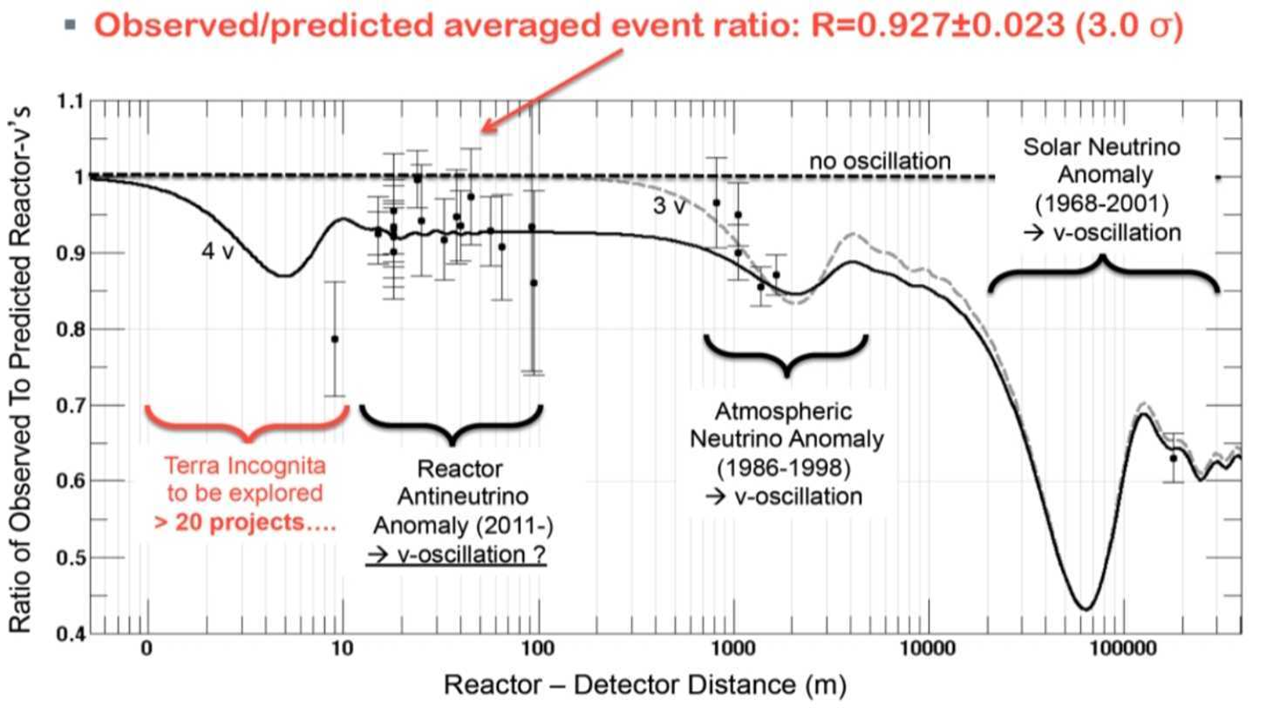
\includegraphics[width=0.8\linewidth]{Chapter2/Figs/neutrino4PlotStretched.jpg}
 \captionof{figure}[Possible areas of interest for sterile neutrinos according to Neutrino-4.]{The possible process of oscillations to a sterile state at small distances of Neutrino-4 from the active zone of the SM-3 reactor other $\nu_e$ oscillations and anomalies are shown for completeness. From \cite{neutrino4_2021}.} 
 \label{fig:neutrino4Plot}
\end{figure}

%There is also a micro boone internal note that may be of use for sterile neutrinos\cite{microboonecollaboration2021search} 

\section{Reactor Neutrino Anomaly And 5\,MeV ``Shoulder''}
% In figure \ref{fig:neutrino4Plot} between 10\,m -- 100\,m there is an area dedicated to the reactor neutrino anomaly. This anomaly was \cite{mention_anAnomaly_2011}, 
% \\\\(papers: double chooz paper \cite{Abe_2012}, reno paper \cite{reno_may_2012}, Daya Bay paper \cite{dayaBay2016_anFlux}, rmills paper \cite{Hayes_implicationsShoulder_2015}, neutron energies on fission spectra \cite{littleJohn_fissionAnSpectra_2018}, Revealing fine an structure from a reactor \cite{AaSonzogni_fineAnSpectra_2017}, microBoone serach \cite{microboonecollaboration2021search}, \cite{Ashenfelter_PROSPECT_2016}).  
Modelling reactor neutrinos is also an active field of research. There are multiple data bases that describe neutrino energies. For example there are the Huber-Muller, Huber-Haag, JEFF-3.1.1, and ENDF/B-VII.1 spectra \cite{Hayes_implicationsShoulder_2015}. These spectra and others like them help to produce an expected neutrino rate. The expected neutrino theory/data ratio should be $\sim 1$, but it is not. Figure \ref{fig:neutrino4Plot} shows between the range from 10\,m -- 100\,m the expected neutrino averaged rate is 0.927 $\pm$ 0.023 to within $3 \sigma$ \cite{neutrino4_2021}. This is the ongoing ``Reactor Neutrino Anomaly'' \cite{mention_anAnomaly_2011}.  This anomaly is possible evidence for a fourth sterile neutrino \cite{mention_anAnomaly_2011}. But considering that the anomaly maybe due to incomplete modelling it is not definitive proof. %But the existence of sterile neutrinos is still awaiting conformation and replication at time of writing.
\\\\In addition, there is the 5\,MeV ``shoulder'' or ``bump.'' This ``bump'' is an excess at $\sim$~5\,MeV in the measured reactor neutrino rates as shown by figure \ref{fig:5MevBumps_DB_R_DC}. The Daya-Bay collaboration has found a 5\,\%~--~10\,\% deviation in their measured anti-neutrino flux between 4.5\,MeV and 5.5\,MeV when compared to the Huber-Muller prediction (figure \ref{subFig:DayaBay5MevBump}. This excess at $\sim$~5\,MeV has been verified up to 4$\sigma$ \cite{dayaBay2016_anFlux}, and has also been observed by the RENO collaboration (figure \ref{subFig:Reno5MevBump}) \cite{Hayes_implicationsShoulder_2015} \cite{dayaBay2016_anFlux} \cite{reno_recentResults_2014}. Although the Double Chooz comparison (figure \ref{subFig:DoubleChooz5MevBump}) is less pronounced depending on the chosen data base \cite{Hayes_implicationsShoulder_2015}. It has been suggested that deviations in the anti-neutrino spectrum could be caused by decay of certain nuclei (namely $^{95}\textrm{Y}$, $^{98,101}\textrm{Nb}$ and $^{102}\textrm{Tc}$). But to test this hypothesis a new generation of detectors such as PROSPECT \cite{Ashenfelter_PROSPECT_2016} will be required. As they will allow for 0.1\,MeV binning or less as opposed to the current 0.25\,MeV binning (i.e better energy resolution) \cite{AaSonzogni_fineAnSpectra_2017}. Both of these effects will have an impact on the results of VIDARR as the detector will likely be deployed at $\sim$ 50\,m from the reactor core. The observed/predicted neutrino rate is expected to be $\sim$~0.93 of what the current reactor models suggest and there will likely be a bump at 5\,MeV in the data sets when compared to current reactor models. These effects will likely be in any reactor spectra that VIDARR measures and as they are expected the impact should be minimal or accounted for.
%This 5\,MeV bump was shown by the Daya-Bay collaboration by $\sim 4 \sigma$ in the 4\,MeV -- 6\,MeV range when comparing to the Huber-Muller spectrum \cite{dayaBay2016_anFlux} (see figure \ref{subFig:DayaBay5MevBump}) this bump is also clearly seen by the  RENO collaboration (figure \ref{subFig:Reno5MevBump}) \cite{Hayes_implicationsShoulder_2015} \cite{dayaBay2016_anFlux} \cite{reno_recentResults_2014}

\begin{figure}[!h]
\centering
\begin{subfigure}{.48\textwidth}
  \centering
  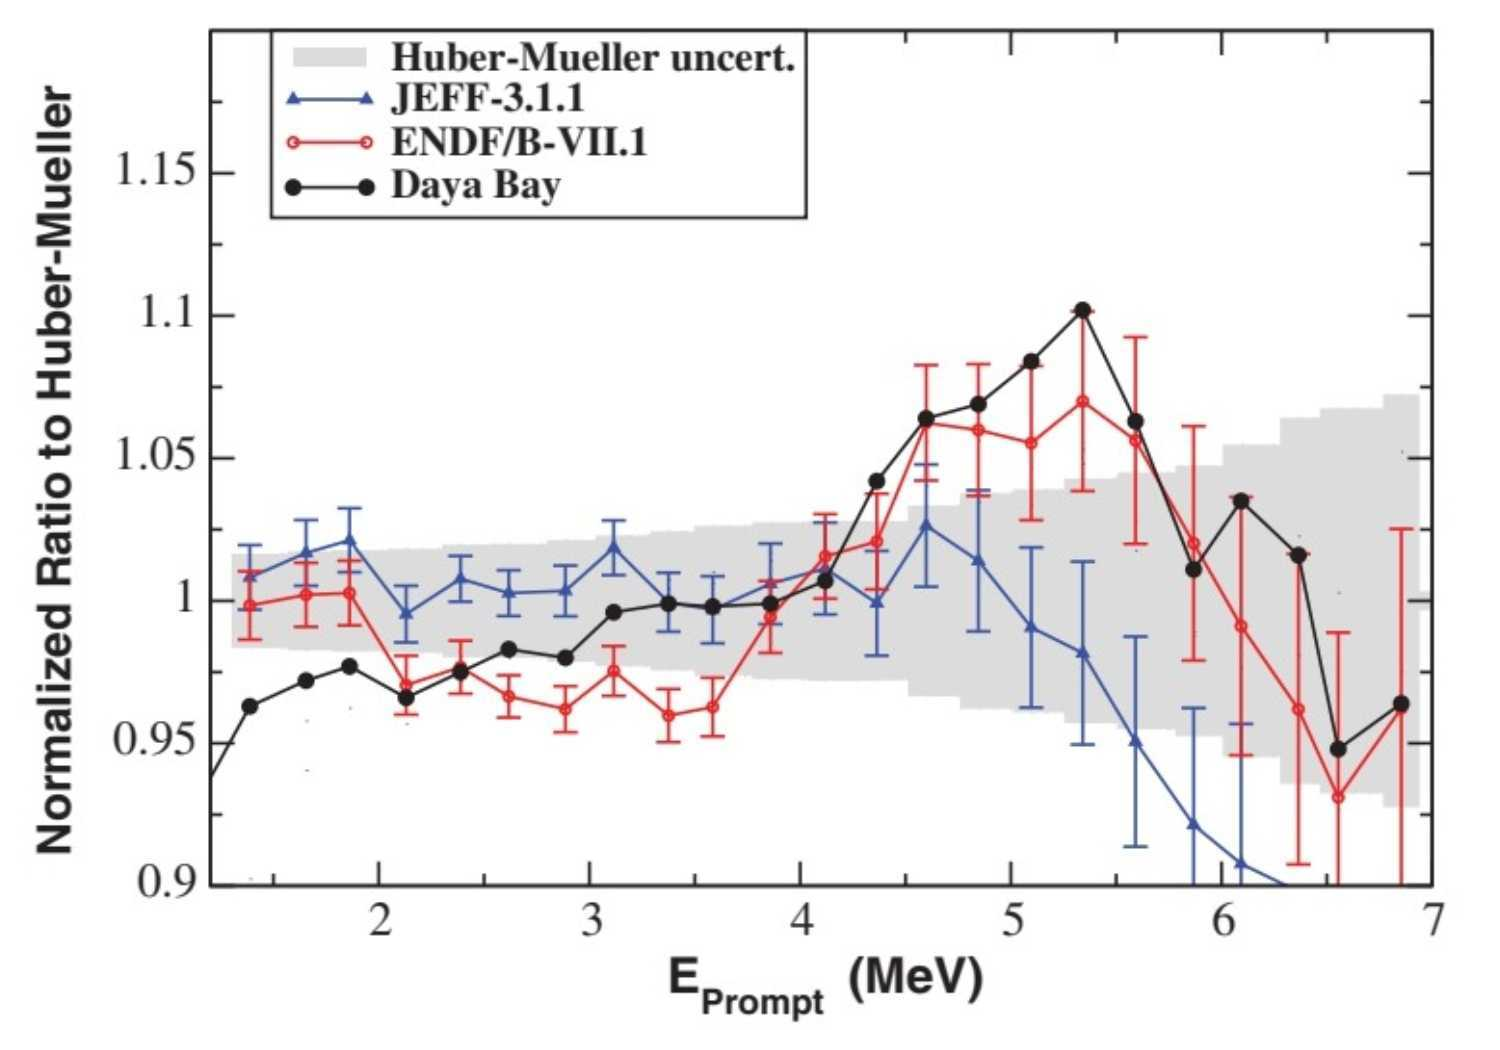
\includegraphics[width=\linewidth]{Chapter2/Figs/Raster/huberMueller_DayaBay_Rmills2015.png}
  \captionsetup{width=.9\linewidth}
  \caption{}
  \label{subFig:DayaBay5MevBump}
\end{subfigure}%
\begin{subfigure}{.48\textwidth}
  \centering
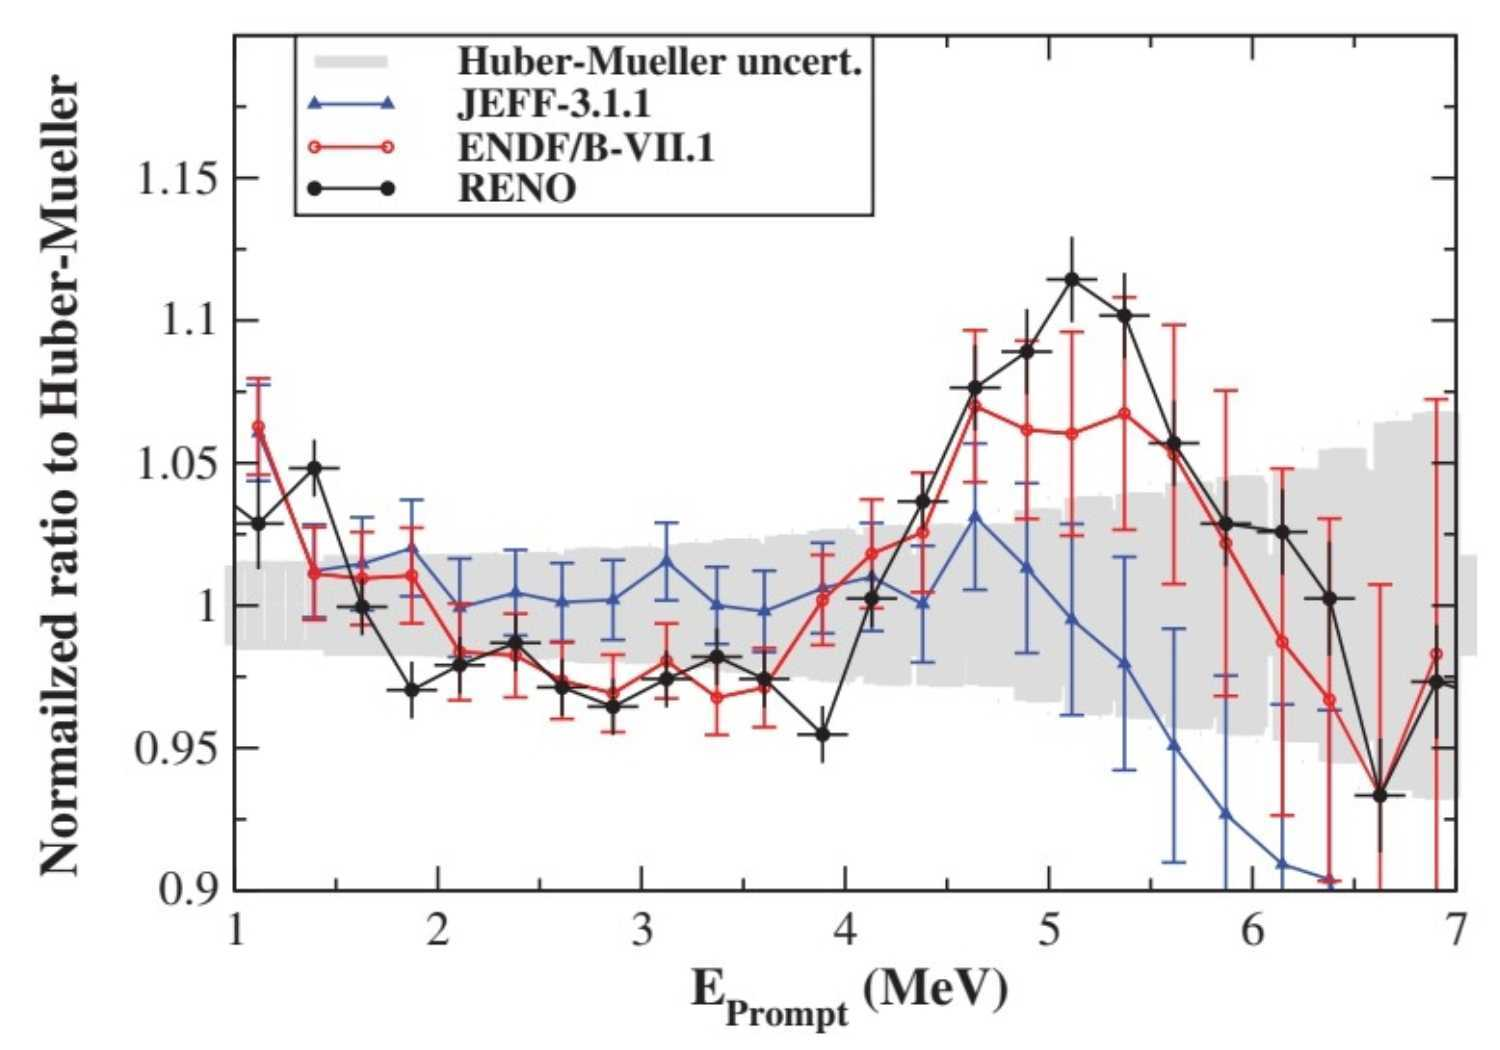
\includegraphics[width=\linewidth]{Chapter2/Figs/Raster/huberMueller_Reno_Rmills2015.png}
  \captionsetup{width=.9\linewidth}
  \caption{}
  \label{subFig:Reno5MevBump}
\end{subfigure}
\begin{subfigure}{.48\textwidth}
  \centering
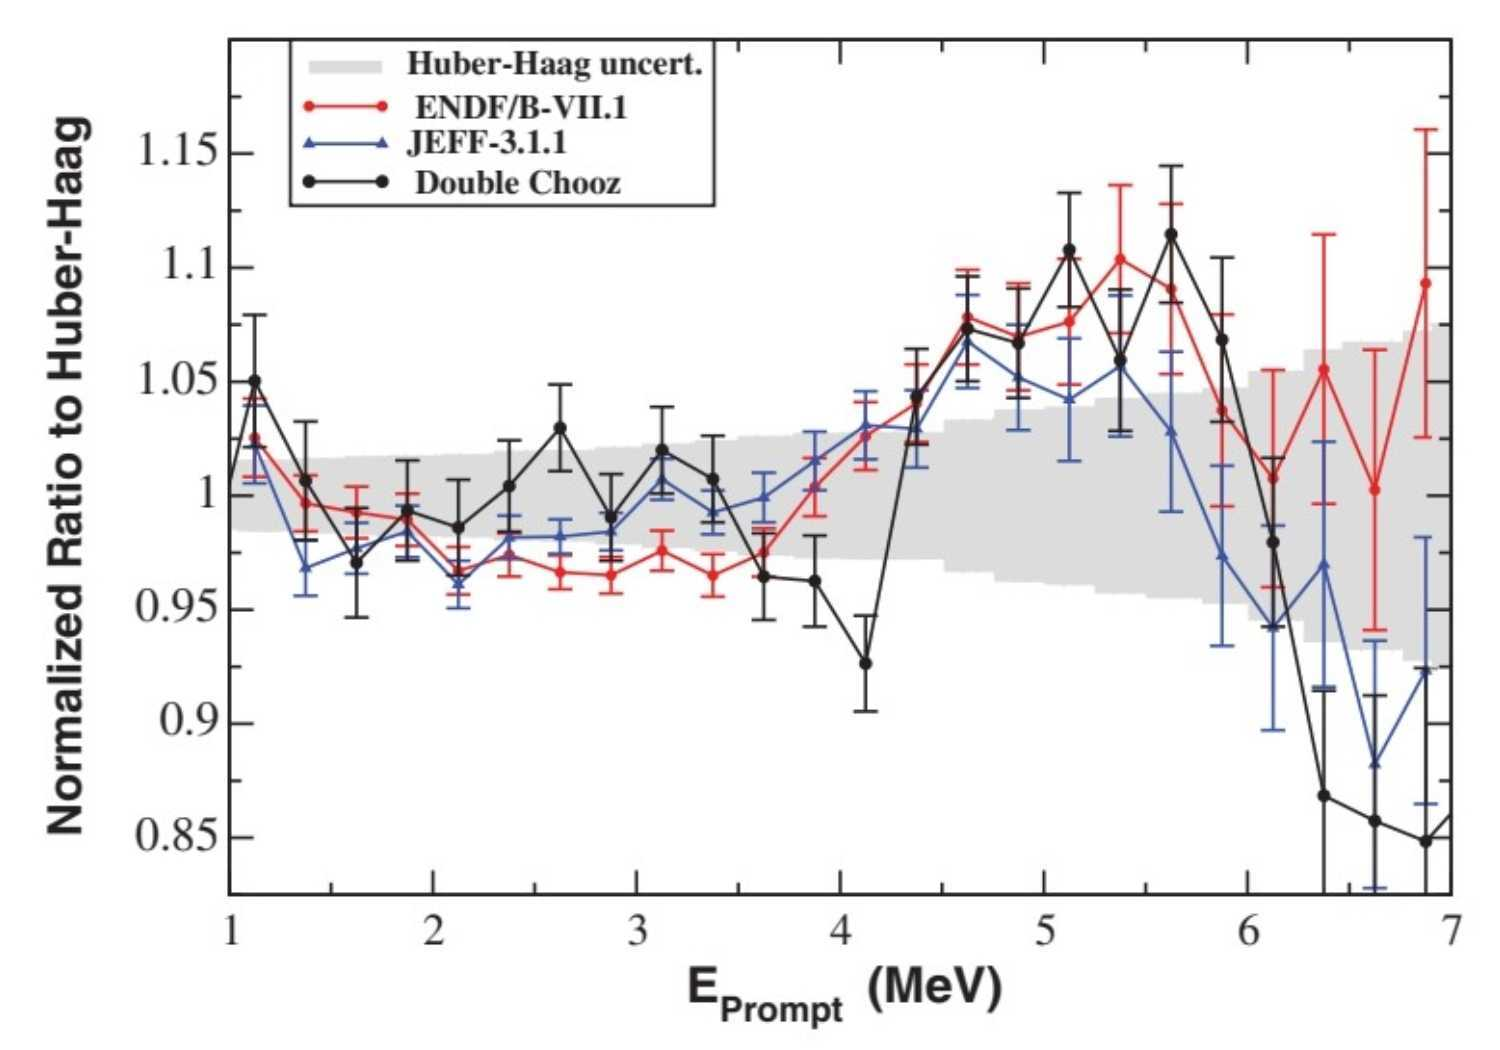
\includegraphics[width=\linewidth]{Chapter2/Figs/Raster/huberHaag_DoubleChooz_Rmills2015.png}
  \captionsetup{width=.9\linewidth}
  \caption{}
  \label{subFig:DoubleChooz5MevBump}
\end{subfigure}
\caption[The 5\,MeV ``shoulder'' for differing experiments.]{The 5\,MeV ``shoulder'' for differing experiments. In (a) the Huber-Mueller spectrum is compared to the Daya Bay results \cite{dayaBay2016_anFlux}. In (b) the Huber-Mueller spectrum is compared to the RENO results \cite{reno_recentResults_2014}. In (c) the Huber-Haag spectrum is compared to the Double Chooz results \cite{abe2014improved}. In all cases a clear peak at 5\,MeV can be seen. However, differing data bases such as JEFF-3.1.1 and ENDF/B-VII.1 can exacerbate or flatten the peak. These are in the window $E_\nu$ = 2--8\,MeV ($E_\nu \approx E_{\textrm{prompt}}$ + 0.782\,MeV). From  \cite{Hayes_implicationsShoulder_2015}.}
\label{fig:5MevBumps_DB_R_DC}
\end{figure} 

%!TEX root = ../thesis.tex
%*******************************************************************************
%****************************** Third Chapter **********************************
%*******************************************************************************

% **************************** Define Graphics Path **************************
\ifpdf
    \graphicspath{{Chapter3/Figs/Raster/}{Chapter3/Figs/PDF/}{Chapter3/Figs/}}
\else
    \graphicspath{{Chapter3/Figs/Vector/}{Chapter3/Figs/}}
\fi

%*******************************************************************************
%****************************** Second Chapter *********************************
%*******************************************************************************

\chapter{The RMon and VIDARR Detectors}\label{Chp:ThePrototypeDetector}
This chapter will discuss the prototype VIDARR detector (RMon) and the on going upgrade of that detector into VIDARR proper. In addition, the initial basis for both detectors the T2K ND 280 will also be covered. As well as a brief mentioning of the background at reactor sites. The upgrade progressed steadily until the COVID-19 pandemic. Despite the ongoing uncertainty the detector has had a $\sim$ 50\,\% increase in mass and new cooling and containment. At time of writing the electronics are currently awaiting upgrade. 

\section{Technology And Results Of RMon}
This thesis will cover consider RMon and the upgraded detector VIDARR. RMon the original prototype detector was re-purposed technology from the T2K ND280 (Near Detector (at) 280\,m) Electromagnetic Calorimeter (ECal) \cite{Allan_2013}. The VIDARR detector uses the same detection media but upgraded electronics and containment which will be referred to as the VIDARR detector. This section will focus on the RMon detector.
\\\\The ND280 detector located at JPARC for the T2K experiment was particularly used to study the $\nu_\mu$ beam used for neutrino oscillation measurements. The detector consists of central sub-detectors comprising of time guarded scintillator bus fine-grained detectors (FGDs) and time projection chambers (TPCs) using lead as the interaction medium surrounded by ECals to stop and measure particles leaving the central detector (see figure \ref{fig:nd280Fig}). The ECals used lead sheets as a conversion material as well as a secondary target. 
%\\\\As it is the basis for the other detectors a quick overview of the T2K ND280 ECal will be required. The ND280 is a series of detectors from the neutrino oscillation experiment T2K which relies on a $\nu_\mu$ beam entering the detector shown in figure \ref{fig:nd280Fig}. This detector was comprised of several different detectors including time projection chambers (TPCs) and fine-grained detectors (FGDs) and electromagnetic calorimeters (ECals) \cite{Allan_2013}. The ECals are of particular interest as they are the basis for the RMon and VIDARR detector due to their robust design inert nature and high precision.  

\begin{figure}[!h]
 \centering
 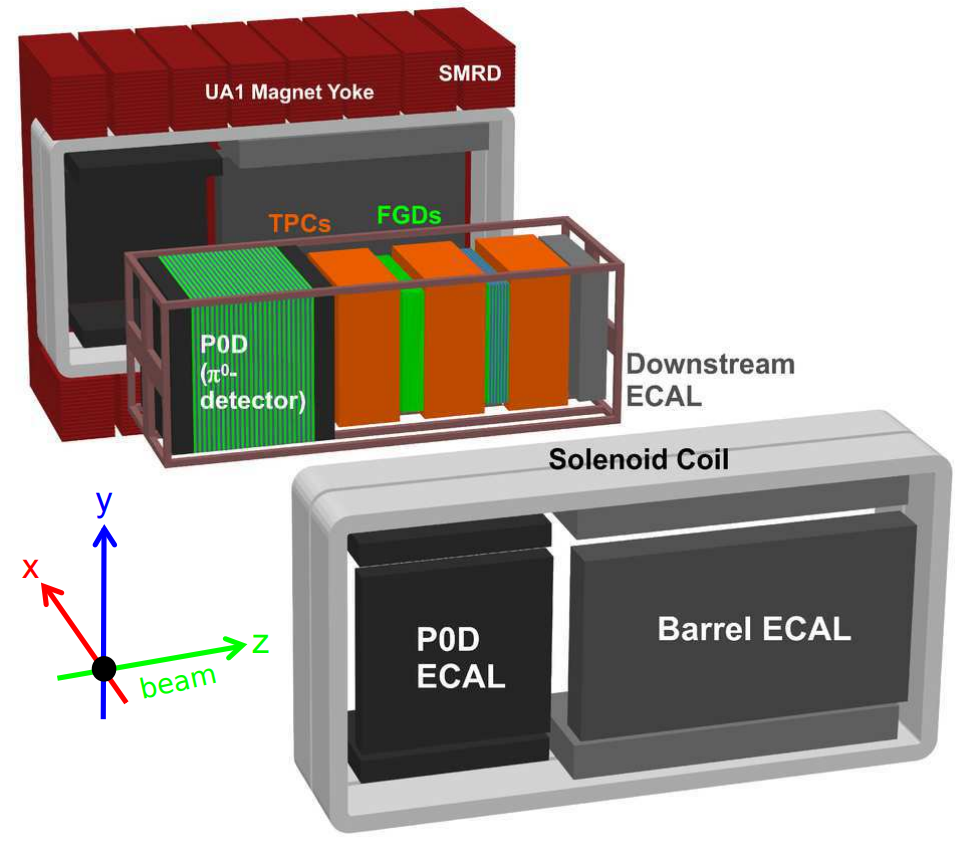
\includegraphics[width=\linewidth/2]{Chapter2/Figs/Raster/ND280Fig.png} 
 \captionof{figure}{Diagram of the ND280 detector. From \cite{Allan_2013}} %~can be used as a kind of place holder in latex
 \label{fig:nd280Fig}
\end{figure}

The T2K ECals were made from plastic scintillating bars measuring 4\,cm by 1\,cm with varying lengths arranged in alternating layers at 90 degrees to each other (see figure \ref{fig:vidarrDiagram}) \cite{Allan_2013}. Wavelength shifting (WLS) fibres were placed in the centre of the scintillating bars to measure light collection which shift the wavelength from blue to green to increase the quantum efficiency of the sensors \cite{Allan_2013}. These wavelength shifting fibres are then connected to multi-pixel photon counters (MPPCs) which produce pulses of charge $\sim$ proportional to the number of photons detected. This in turn is related to the energy deposited in the bar. This signal is then read in by Trip-T front-end electronic boards (TFBs) which integrates the charged received into an array of 23 time buckets of programmable width (480\,ns for ND280, 1.5\,$\mu$s for RMon). 
\\\\However, a crucial difference between the ECals of the ND280 and the RMon detector is that the lead sheets have been replaced with a layer of Mylar coated with gadolinium sulphate so that neutrons produced in IBD (equation \ref{inverse_beta_decay}) are captured. RMon was also designed to fit inside of a shipping container each bar having a length of 152\,cm and the whole detector measuring 152\,cm $\times$ 152\,cm with 49 layers of plastic scintillating bars giving a height of 49\,cm and a total of 1862 bars. The electronic systems were also adapted from the T2K ECal. They were configured such that they were triggered from a neutron-induced gadolinium cascade from IBD by looking for a large number of hits in the trigger cycle. Of the 23 cycles 0 -- 17 are considered "prompt" and cycle 18 is the trigger cycle. Cycles 19 -- 22 were left as control so that they could be compared in case time-dependent issues arose from the altered system. As will be discussed later in chapter \ref{chp:cosmicMuonTomography} these cycles were used to diagnose a time dependant issue with the cosmic $\mu$ data set.
\\\\$\Bar{\nu_e}$s are detected by their absorption by a proton and decay into a $e^+$ and a neutron as shown in figure \ref{fig:inverse_beta_diagram}. The e$^+$ and subsequent annihilation $\gamma$ rays leave short tracks in the detector. Th annihilation particles may be used to distinguish the e$^+$ from the $\beta$ decay e$^-$ backgrounds. The neutron interaction shown in figure \ref{fig:inverse_beta_diagram} the neutron is absorbed by the Gadolinium sheets in the detector which then causes an 8\,MeV $\gamma$ cascade which will be expanded upon in section \ref{sec:GEANT4Simulation_modellingGadolinium}. Gadolinium is one of the most preferred neutron capture agents due to it's extremely high capture cross-section of its isotopes especially $^{155}$Gd ($\sigma$ = 61000 b) and $^{157}$Gd ($\sigma$ = 255000 b) \cite{gadFoilsThermalNeut}. 

\begin{figure}[!h]
\centering
  \centering
  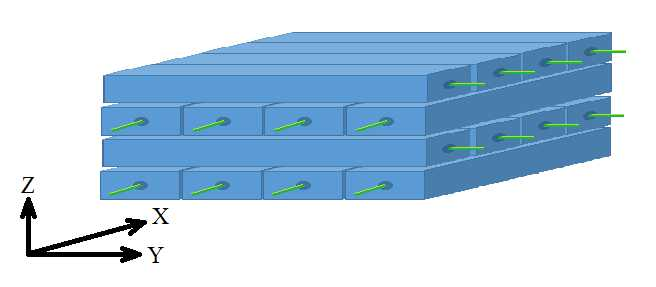
\includegraphics[width=0.6\linewidth]{Chapter2/Figs/Raster/VIDARR_diagram.jpeg}
  \captionof{figure}{A cutaway diagram showing the structure of the RMon and VIDARR detectors. The segments are 4\,cm wide $\times$ 152\,cm long by 1\,cm tall. The Gadolinium sheets in-between the RMon/VIDARR segments are not shown. From \cite{GeorgeHoltDiagram}.}
  \label{fig:vidarrDiagram}
\end{figure}

The original detector was deployed at the Wylfa power station in Anglesey Wales for an 18-month period. This run proved successful in measuring the power from the reactor to within good agreement of the measured reactor flux. Figure \ref{fig:prototypeMeasumentFlux} compares the measured $\bar{\nu_e}$ flux with the reported power output and shows how good the agreement is. A measured anti-neutrino rate of 172.1 $\pm$ 4.6 candidates per day is observed when the reactor is off and 203.7 $\pm$ 19.6 when the reactor is on \cite{Carroll_2018}. These results line up with the expectation from the SONGS1 deployment (figure \ref{subFig:reactorPowerSongsS1}) where a increase in $\bar{\nu_e}$ candidates correlates with an increase in reactor power. %Unfortunately due to cooling issues with the RMon detector the reactor shutdown was not observed. This is one of the main motivating factors behind the upgrade of the detector as the first generation MPPCs and repurposed electronics were susceptible to high levels of noise if the temperature was not carefully controlled. 
\begin{figure}[!h]
 \centering
 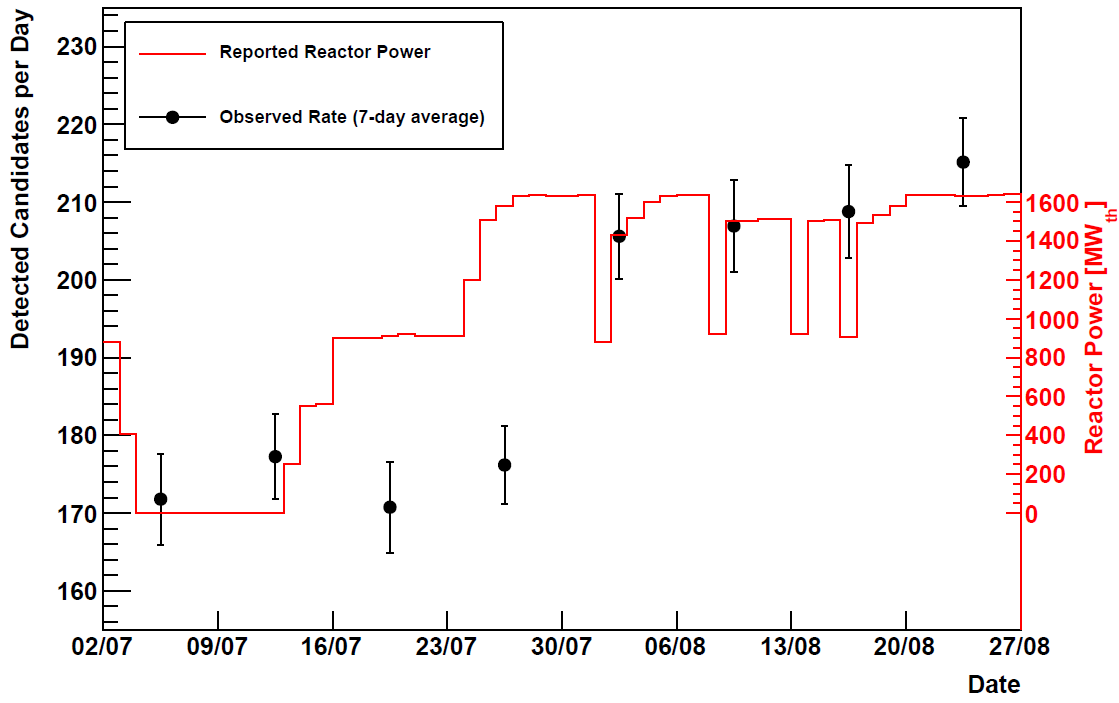
\includegraphics[width=0.7\linewidth]{Chapter2/Figs/Raster/prototypeMeasureOnFig.png} 
 \captionof{figure}{Measured anti-neutrino flux compared to the power generation from the Wylfa power station. The increase in $\bar{\nu_e}$ candidates correlates with an increase in power generation. These results demonstrate the success of the RMon deployment and technology. From \cite{Carroll_2018}} %~can be used as a kind of place holder in latex
 \label{fig:prototypeMeasumentFlux}
\end{figure}

Considering the re-purposed nature and rapid development cycle of RMon the deployment at Wylfa and subsequent neutrino measurement (see figure \ref{fig:prototypeMeasumentFlux}) is a good demonstration of the detection media and experimental setup. However, whilst these results are highly encouraging the response measurement can still be improved, for example the SONGS1 measurement is more accurate (see figure \ref{fig:reactorPowerAndRefuelingSongsS1}). In addition, the PANDA collaboration has been able to measure a neutrino spectrum the from Ohi power plant at a distance of $\sim$ 50\,m \cite{IIRIE_Panda_2021} (see figure \ref{subFig:Panda_spectrumOfIbdCandidates}). With an upgraded version of the RMon detector it should be possible to achieve similar results to SONGS1 and PANDA and might be possible to distinguish particular isotopes of nuclear fuel.

\section{Studies Of Background At Reactor Sites}
Backgrounds at reactor sites are important to quantify as it helps to guide shielding requirements. The results from SONGS1, PANDA, and RMon all show low count rates per day of $\sim$ 100 per ton. These low count rates necessitate a good understanding of background. The PROSPECT experiment has done a  study looking into the background at two research reactor locations difference between the National Bureau of Standards Reactor (NBSR) at NIST and the High Flux Isotope Reactor (HFIR) at ORNL \cite{Ashenfelter_2016}. Another site was considered by the PROSPECT the ATR at INL but the increased altitude of that site leads to a significantly higher cosmogenic neutron flux \cite{Ashenfelter_2016}. An example of how reactors affect the background can be seen in figure \ref{fig:Prospect_NSBR_gammaSpec} which shows how the $\gamma$ spectrum varies when the NBSR is on and off, it shows how the spectrum between 3\,MeV -- 9\,MeV is mostly dominated by reactor noise. 
\\\\Another component is neutron measurements caused by the reactor which is shown in figure \ref{fig:prospectNeutronMap} for thermal neutrons which are an issue for $\bar{\nu_e}$ detectors but should be somewhat negated through robust e$^+$ identification and accurate double coincident measurements. Another more important background is fast neutrons because they cause a false double coincident signal by potentially interacting with protons and then thermalising and being absorbed. The measurement of cosmogenic neutron background has been done by JEDEC in 2006 \cite{JEDEC_2006} as well as PROSPECT in figure \ref{fig:Prospect_HFIR_NBSR_nearFarPlots} which shows similar rates at different locations this is unsurprising as this is largely a function of altitude more than any other factor \cite{Ashenfelter_2016}. \\\\However, a type of background that is easy to mitigate (for VIDARR) but also extremely useful are cosmic $\mu$. Cosmic $\mu$ have a large number of events of $\sim$ 119\,s$^{-1}$m$^{-2}$ according to the CRY library \cite{ieee_cry_2007} (also see figure \ref{fig:CRY_rates}). These particles can be detected by very simple detector requiring only a series of paddles as seen in figure \ref{fig:Prospect_MuonPaddels}. This cosmic $\mu$ background is useful as they are highly penetrating particles tracks that can be approximated to be straight lines (later discussed in chapter \ref{chp:cosmicMuonTomography}). The range of angles incident cosmic $\mu$ posses make them useful for tomographic purposes as will be discussed in chapter \ref{chp:cosmicMuTelescopes}. % The angles of incidence of cosmic $\mu$ can have many useful applications and as such these cosmic $\mu$ should not be excluded as mere noise as will be shown in section \ref{sec:cosmicMuTelescopes}.


\begin{figure}[!h]
\centering
\begin{minipage}{.45\textwidth}
  \centering
  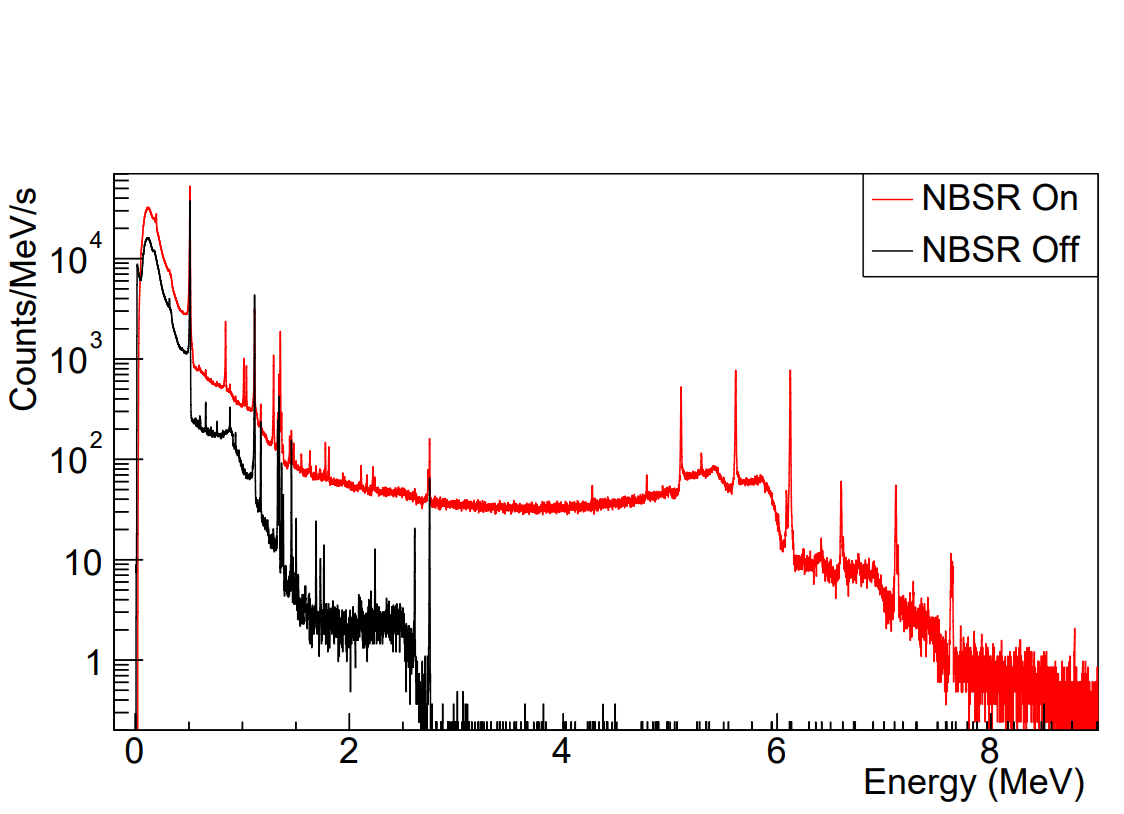
\includegraphics[width=\linewidth]{Chapter2/Figs/Raster/Prospect_NSBR_gammaSpec.png}
  \captionof{figure}{Example HPGe $\gamma$-ray spectra taken with the NBSR on and off. Prominent lines, and associated escape peaks and Compton continua, are evident. From \cite{Ashenfelter_2016} (table 2 in \cite{Ashenfelter_2016} shows line sources).} 
  \label{fig:Prospect_NSBR_gammaSpec}
  \vspace*{3.1635cm} %1line = 0.633(3 is recurring)cm  %%% 2lines = 1.2666cm(6 is recurring) %%% 3lines = 1.90cm exactly %%% 5lines is 3.1635cm exactly
\end{minipage}%
\qquad
\begin{minipage}{.45\textwidth}
  \centering
  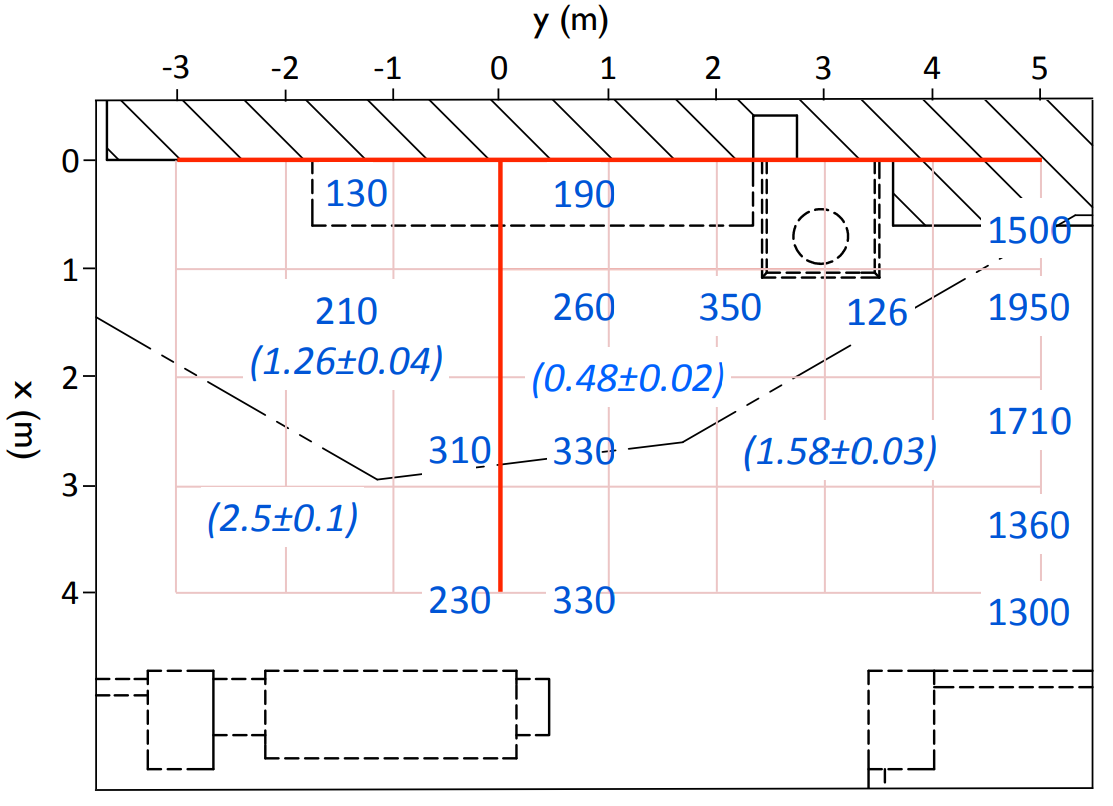
\includegraphics[width=\linewidth]{Chapter2/Figs/Raster/prospectNeutronMap.png} 
  \captionof{figure}{A pictorial representation of neutron dose rates (measured in nSv/h) and thermal neutron rates in italics (cm$^{-2}$ s${^-1}$) at the HFIR near location roughly 15\,cm (z = 0.15) above the floor. Measurements are plotted on a one meter square grid referenced to the reactor wall (x = 0) and the smallest baseline (y = 0). The reactor core is centred at (x,y,z) = (-4.06,0,-3.85). From \cite{Ashenfelter_2016}.}
  \label{fig:prospectNeutronMap}
\end{minipage}
\end{figure}

% \begin{figure}[!h]
%  \centering
%  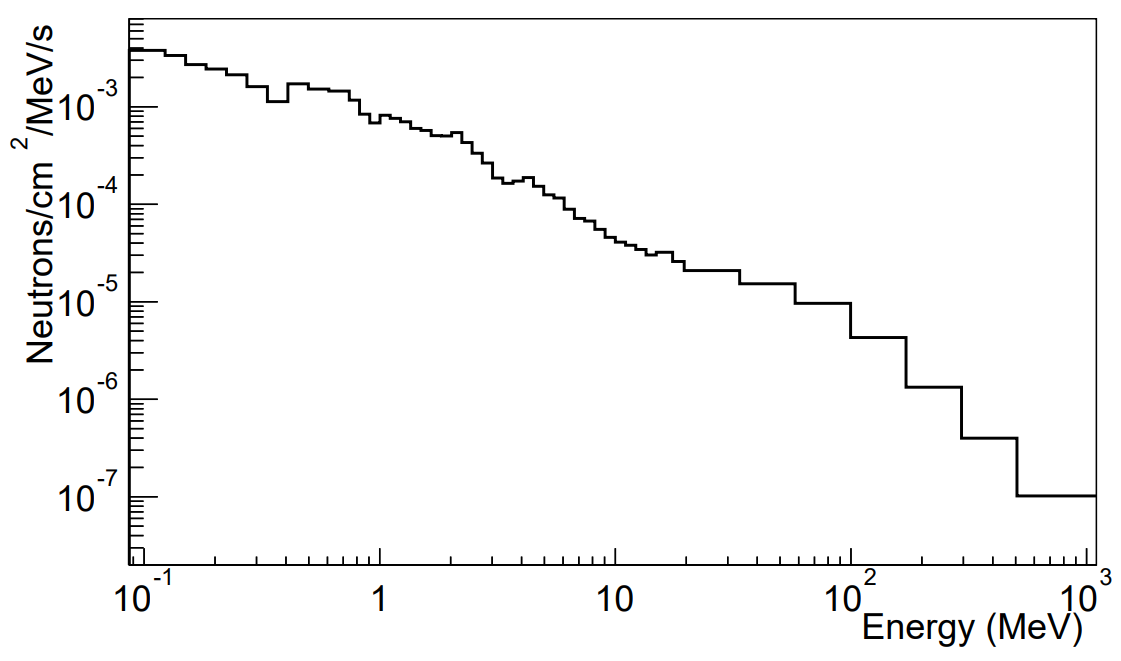
\includegraphics[width=0.7\linewidth]{Chapter2/Figs/Raster/JDEC_neutronSpec.png}
%  \captionof{figure}{The JEDEC standard fast neutron spectrum recorded at sea
% level in New York. From \cite{JEDEC_2006}. } 
%  \label{fig:JDEC_neutronSpec}
% \end{figure}

\begin{figure}[!h]
\centering
\begin{subfigure}{.5\textwidth}
  \centering
  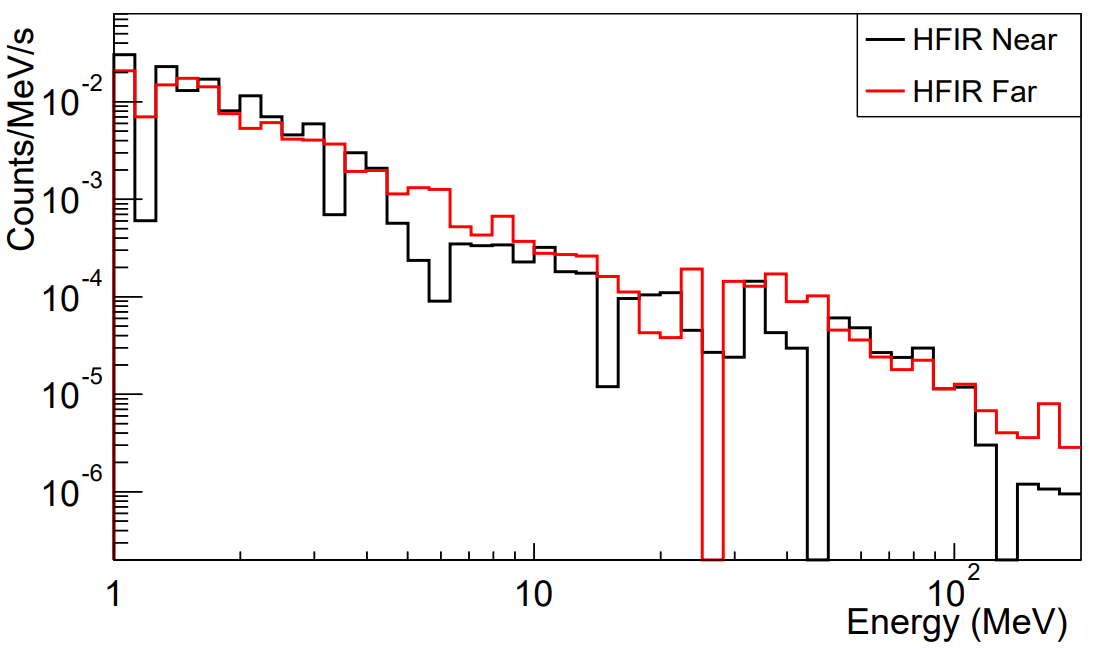
\includegraphics[width=\linewidth]{Chapter2/Figs/Raster/Prospect_HFIR_nearFarPlot.png}
  \captionsetup{width=.9\linewidth}
  \caption{}
  \label{subFig:Prospect_HFIR_nearFarPlot}
\end{subfigure}%
\begin{subfigure}{.5\textwidth}
  \centering
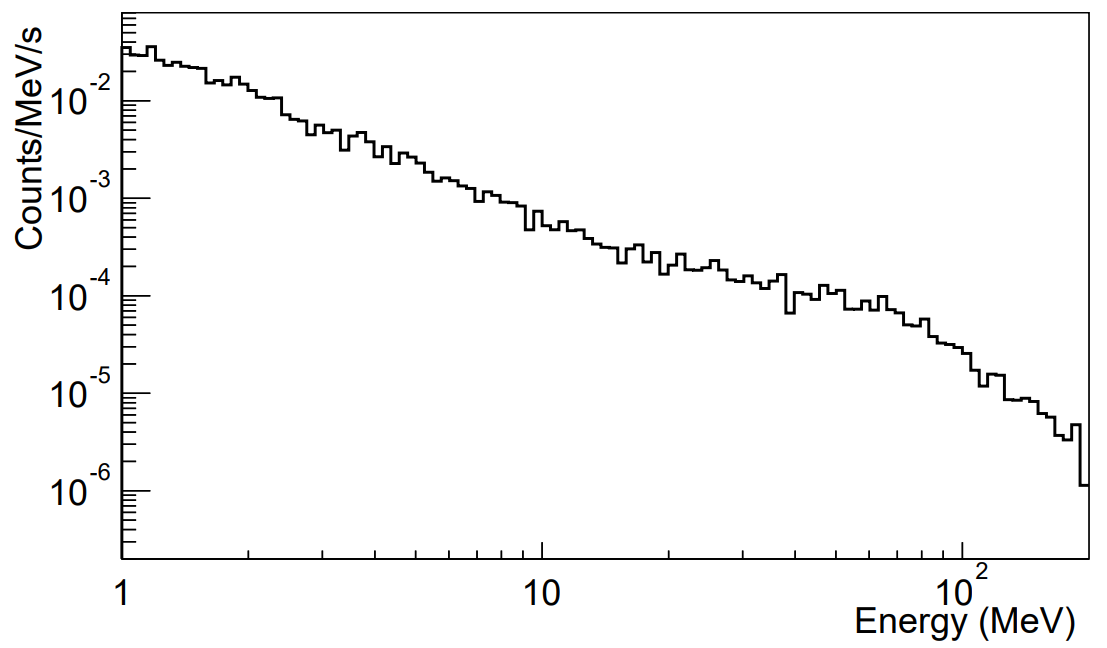
\includegraphics[width=\linewidth]{Chapter2/Figs/Raster/Prospect_NBSR_farPlot.png}
  \captionsetup{width=.9\linewidth}
  \caption{}
  \label{subFig:Prospect_NBSR_farPlot}
\end{subfigure}
\caption{The cosmogenic neutron-induced energy spectrum was recorded at the (a) HFIR near and far locations and (b) NBSR far location. From \cite{Ashenfelter_2016}.}
\label{fig:Prospect_HFIR_NBSR_nearFarPlots}
\end{figure}

\begin{figure}[!h]
 \centering
 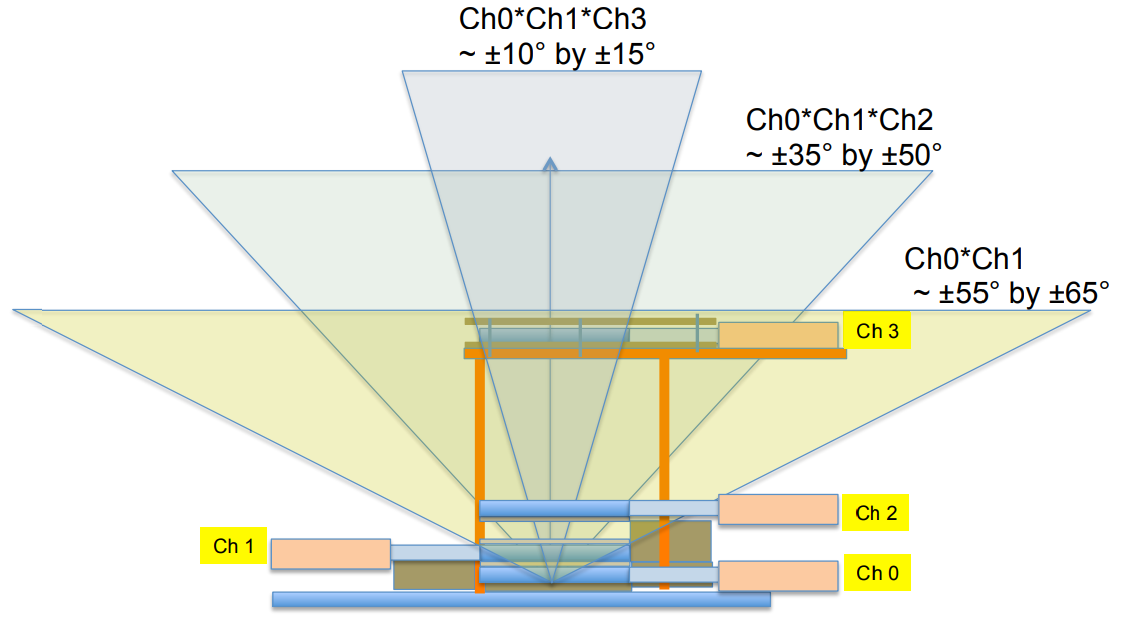
\includegraphics[width=0.7\linewidth]{Chapter2/Figs/Raster/Prospect_MuonPaddels.png}
 \captionof{figure}{The angular acceptances for the $\mu$ telescope instrument
used at all sites is determined by the coincidence requirement enforced
between the 4 plastic scintillator paddles. These detectors were deployed by the PROSPECT experiment at both the NBSR and HFIR sites. From \cite{Ashenfelter_2016}.} 
 \label{fig:Prospect_MuonPaddels}
\end{figure}

\clearpage
\section{The VIDARR Detector Upgrade}\label{sec:theUpgradedDetector}
The deployment of RMon demonstrated that the choice of detector media (scintillating bars Gd doped sheets and wavelength recorded by WLS fibres) worked well. However, the detector would benefit from more mass, higher efficiency sensors and dedicated electronics. The upgraded detector will have 21 more layers than the RMon detector going from 49 to 70 layers and the 3 missing columns on side A are also now instrumented (see figure \ref{fig:detectorUpgradedmassOutlined}). This means the number of channels has increased from 1793 to 2660 which results in a mass increase of $\sim$ 50\,\%, thus improving the fiducial volume of the detector. The increase in layers will increase the amount of the 8\,MeV Gd cascade contained on average in the detector allowing for more effective background reduction when triggering. The MPPCs are also a new generation with 2 $\times$ the efficiency going from RMon to VIDARR. %The increase in layers will not yield a significant increase in e$^+$ efficiency as e$^+$s are effectively contained to a $\sim$ 99\,\% level with both 1793 channels and 2660 channels as they are contained within 1-2 bars.

\begin{figure}[!h]
 \centering
 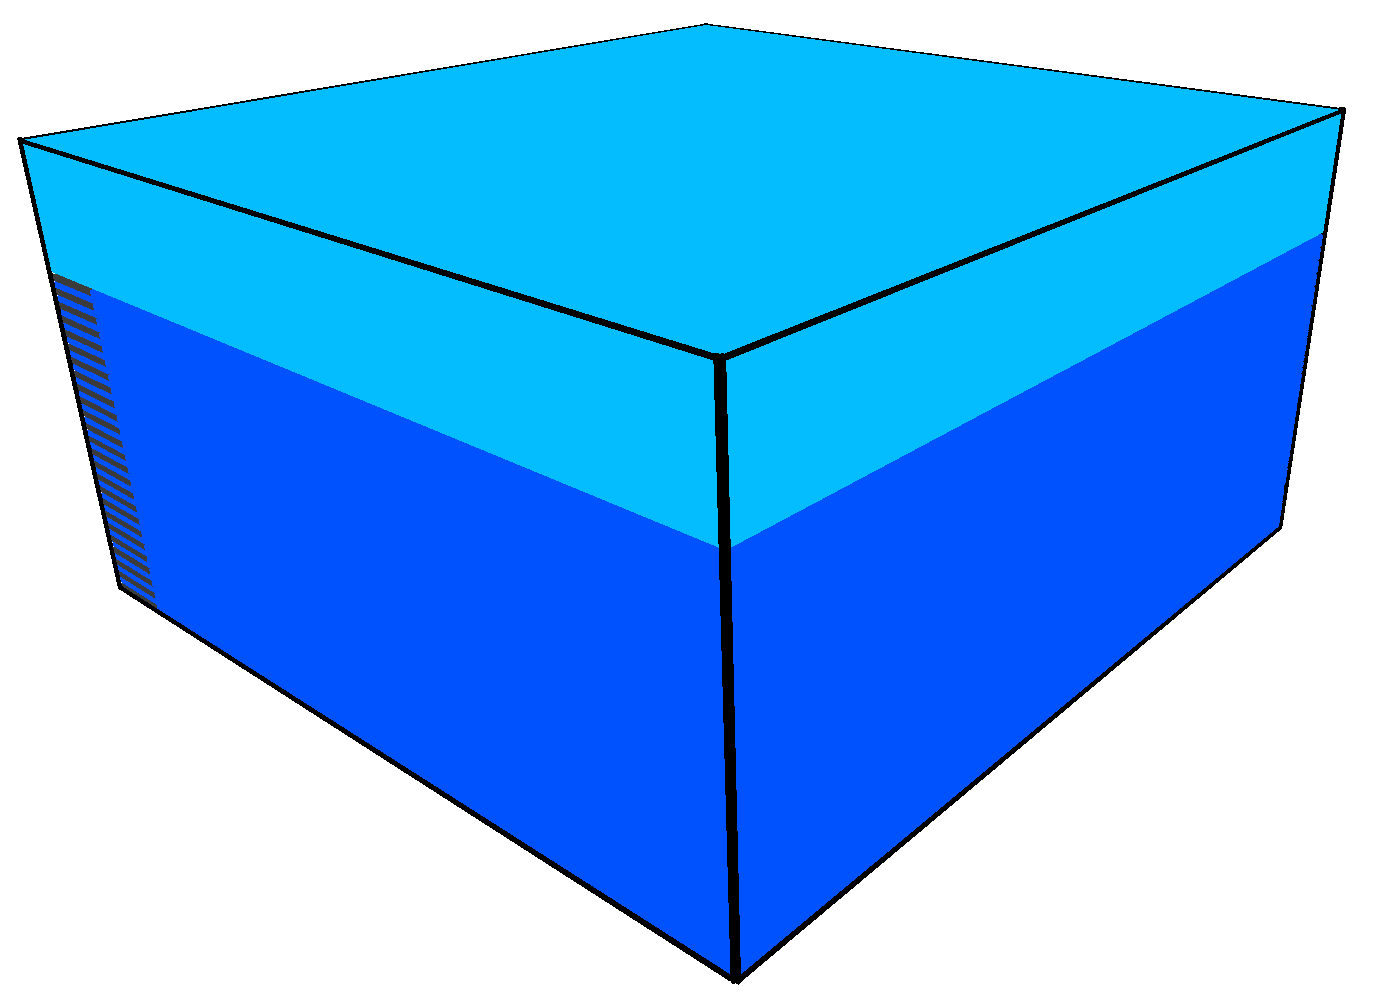
\includegraphics[width=0.5\linewidth]{Chapter3/Figs/detectorUpgradedmassOutlined.png}
 \captionof{figure}{The upgraded detector mass (light blue) on top of the original mass (dark blue). The greyed out channels on the left hand side of side A were those left un-instrumented in the original deployment but are now instrumented in the upgrade.} 
 \label{fig:detectorUpgradedmassOutlined}
\end{figure}

The electronics have been improved significantly when compared to the original detector. The original electronics and sensors were taken from the T2K ECal. The MPPCs were the first generation of this technology with relatively low efficiency and high noise rates compared to the current generation used in the VIDARR detector. The energy resolution of the detector has been greatly improved by using more modern, higher efficiency MPPCs. In addition, the upgraded detector will have channel by channel trigger output to Field-Programmable Gate Array (FPGA) boards that connect with analogue boards in turn connecting to the MPPCs. The use of FPGA boards will allow for more complex trigger functions to be used and trigger on the detector as a whole. This will be achieved by looking at the summed energy and the number of bars hit past each threshold. As will be expanded upon later in section \ref{sec:MachineLearningTrigger} the improvement to energy resolution has a significant effect on the S/N ratio as well. During the analysis the lowest available threshold of $\sim$ 0.1\,MeV was the most effective in distinguishing signal from noise. This improvement is only possible due to the upgraded sensors and electronics. Both generations of MPPCs are highly temperature sensitive, and this did cause stability issues for the RMon detector. %The use of two thresholds as opposed to one on the RMon also proved useful for improving generated neutron efficiency. 
%\\\\A basic cut investigation used a form of machine learning called a support vector machine (SVM) to determine the best cut and which dimensions gave the best separation. The cut was dominated by the number of bars hit at the lower threshold of 0.1\,MeV, the most accurate cut would have been utilising the number of bars hit above 0.1\,MeV and the summed energy above the 0.1\,MeV threshold. However due to the structure of the FPGA boards and their programming it was more prudent to use the number of bars hit above both the 0.1\,MeV thresholds and 0.5\,MeV threshold. The cost in classifier accuracy was minimal and it allowed for faster development of the FPGA firmware. 
\\\\To lessen temperature fluctuations in the VIDARR detector the cooling in and around the detector module has been greatly increased from the RMon prototype. The original detector had six radiator fins on 2 sides of the detector which were primarily aimed at cooling the TFBs on each fin (see figure \ref{fig:detCon002_OldTearAway}). The upgraded VIDARR detector will also have cooling fins which will take heat away from the new boards but on the same 2 sides as the fins, there will also be two new radiators behind the fins which run the width and height of a side figure \ref{fig:detCon_RadiatorConstruction_RadiatorPiping} shows the radiators being constructed. The new active cooling the radiators will provide cooling to the cavity housing to the MPPCs and shield them from heat generated by the active electrons. This will allow for a more consistent temperature and reduce dark noise from the MPPCs below the original detector's levels. In addition temperature monitoring has also been added to ensure the MPPCs are maintained at the correct temperature.

\section{Detector Construction}\label{sec:DetectorConstruction}
The detector construction was a process that was sadly disrupted due to the COVID-19 pandemic which is still ongoing. The detector construction originally started in November of 2018 with the cutting and painting of scintillation bars. This process was completed by December 2018. Also in December of 2018, the original detector was moved out of the shipping container which housed it (figure \ref{fig:detCon000_TakeOut1}). It was then placed inside an ISO class 7 cleanroom opened and disassembled (figure \ref{fig:detCon002_OldTearAway}). The RMon detector had much space that could be further utilised. The internal space of RMon was also filled 1\,m long cables connecting the sensors to the electronics (see figure \ref{fig:detCon002_OldTearAway}). By using the internal shell of RMon more efficiently additional channels and cooling was added. New scintillator was purchased from Fermilab which was $\sim$ twice as long as required. This new scintillator was then cut (figure \ref{subFig:detCon003bb_CuttingScint}) so its dimensions match the old scintillating bars (152\,cm $\times$ 4\,cm $\times$ 1\,cm) and fit exactly inside the detector casing. Once this was done, the edges of the freshly cut scintillator were arranged and painted with TiO$_2$ paint (figure \ref{subFig:detCon005b_PaintingEnds}) to help reflect the light. The cut and painted scintillator were then placed inside the housing for the detector  whilst it was in the cleanroom environment to minimise background/contamination (figure \ref{fig:detCon006_RonInCleanRoom}). 

\begin{figure}[!h]
\centering
\begin{minipage}{.45\textwidth}
  \centering
  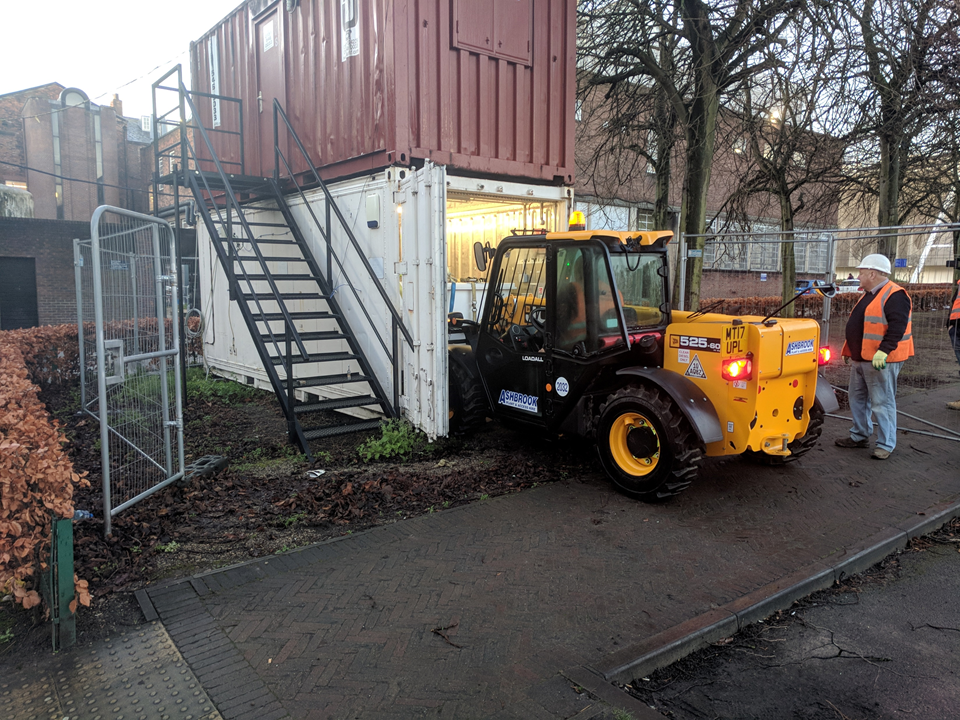
\includegraphics[width=\linewidth]{Chapter3/Figs/Raster/detCon000_TakeOut1.png} 
  \captionof{figure}{The RMon detector being taken out of the original shipping container which was a standard cooled shipping container.}
  \label{fig:detCon000_TakeOut1}
\end{minipage}
\qquad
\begin{minipage}{.45\textwidth}
  \centering
  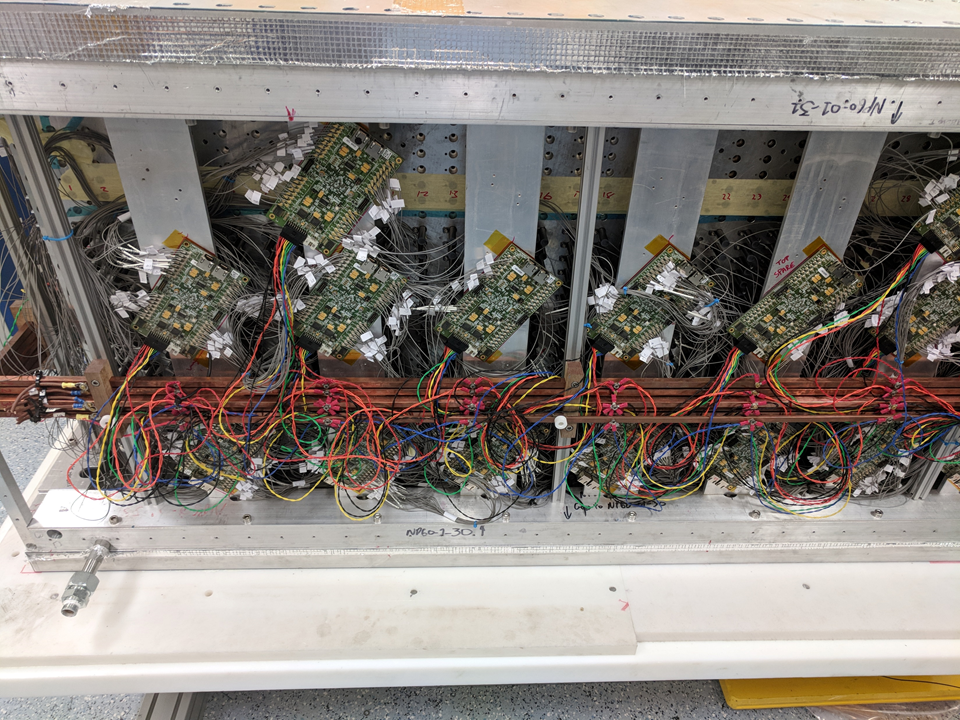
\includegraphics[width=\linewidth]{Chapter3/Figs/Raster/detCon002_OldTearAway.png}
  \captionof{figure}{A view of the electronics in the RMon detector. There is much available space between the boards and the detector itself. The cables are 100\,mm long.} 
  \label{fig:detCon002_OldTearAway}
\end{minipage}%
\end{figure}

\begin{figure}[!h]
\centering
\begin{subfigure}{.5\textwidth}
  \centering
  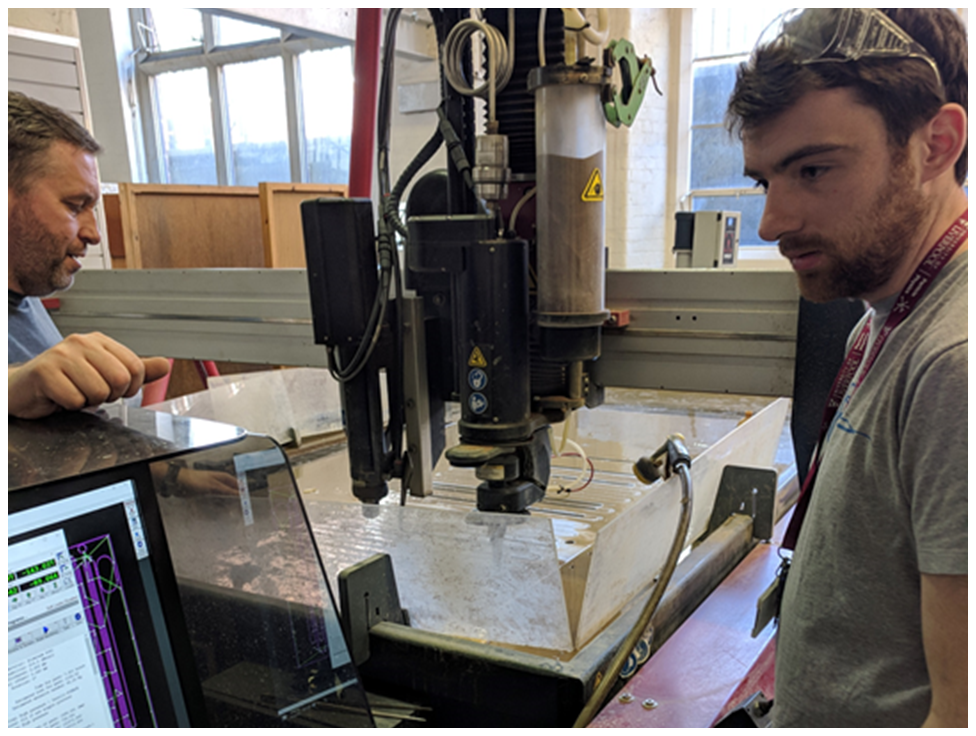
\includegraphics[width=\linewidth]{Chapter3/Figs/Raster/detCon011b_RadiatorConstruction.png}
  \captionsetup{width=.9\linewidth}
  \caption{}
  \label{subFig:detCon011b_RadiatorConstruction}
\end{subfigure}%
\begin{subfigure}{.5\textwidth}
  \centering
  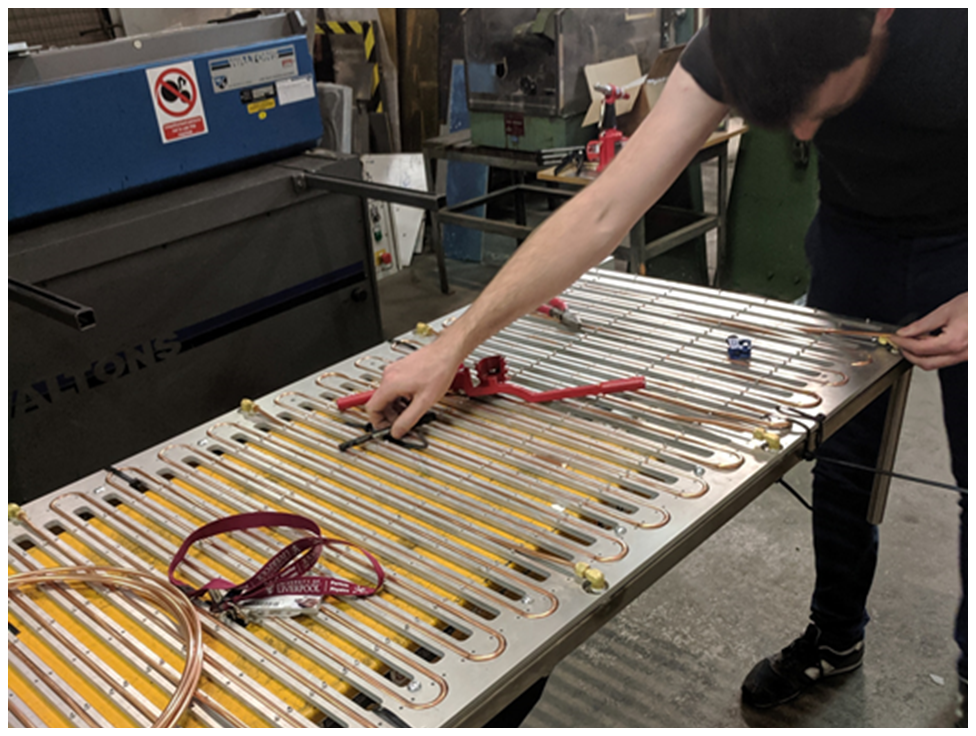
\includegraphics[width=\linewidth]{Chapter3/Figs/Raster/detCon012b_RadiatorPiping.png}
  \captionsetup{width=.9\linewidth}
  \caption{}
  \label{subFig:detCon012b_RadiatorPiping}
\end{subfigure}
\caption{The construction of the new radiator has more active cooling and a larger surface area than the original radiator. The radiator is being cut in (a) and the piping is inserted in (b).}
\label{fig:detCon_RadiatorConstruction_RadiatorPiping}
\end{figure}

\begin{figure}[!h]
\centering
\begin{subfigure}{.5\textwidth}
  \centering
  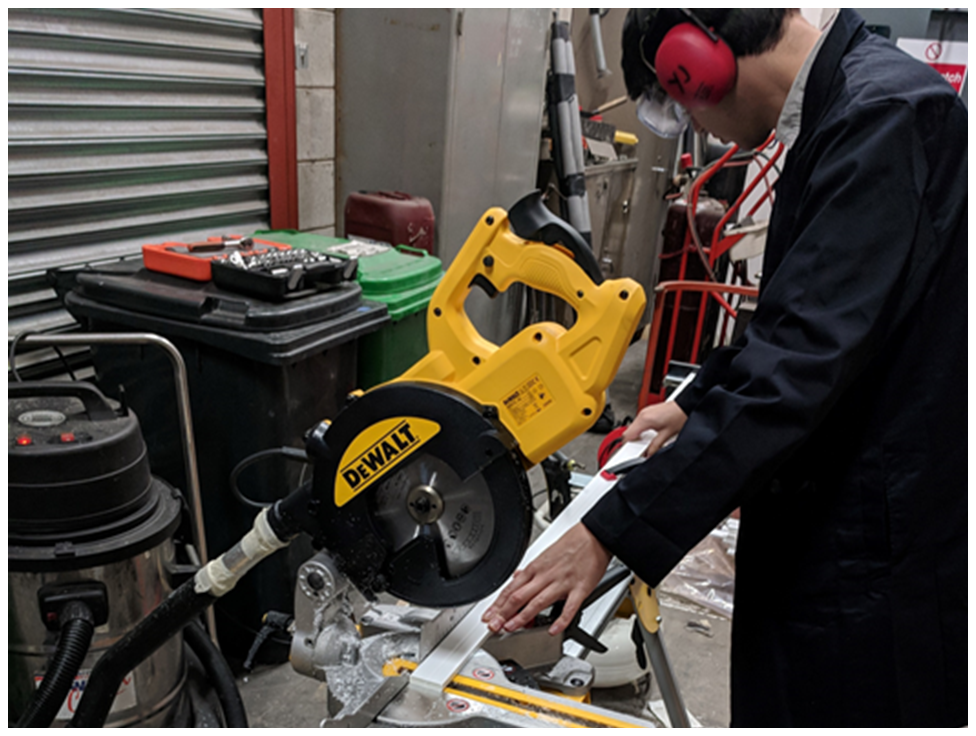
\includegraphics[width=\linewidth]{Chapter3/Figs/Raster/detCon003bb_CuttingScint.png}
  \captionsetup{width=.9\linewidth}
  \caption{}
  \label{subFig:detCon003bb_CuttingScint}
\end{subfigure}%
\begin{subfigure}{.5\textwidth}
  \centering
  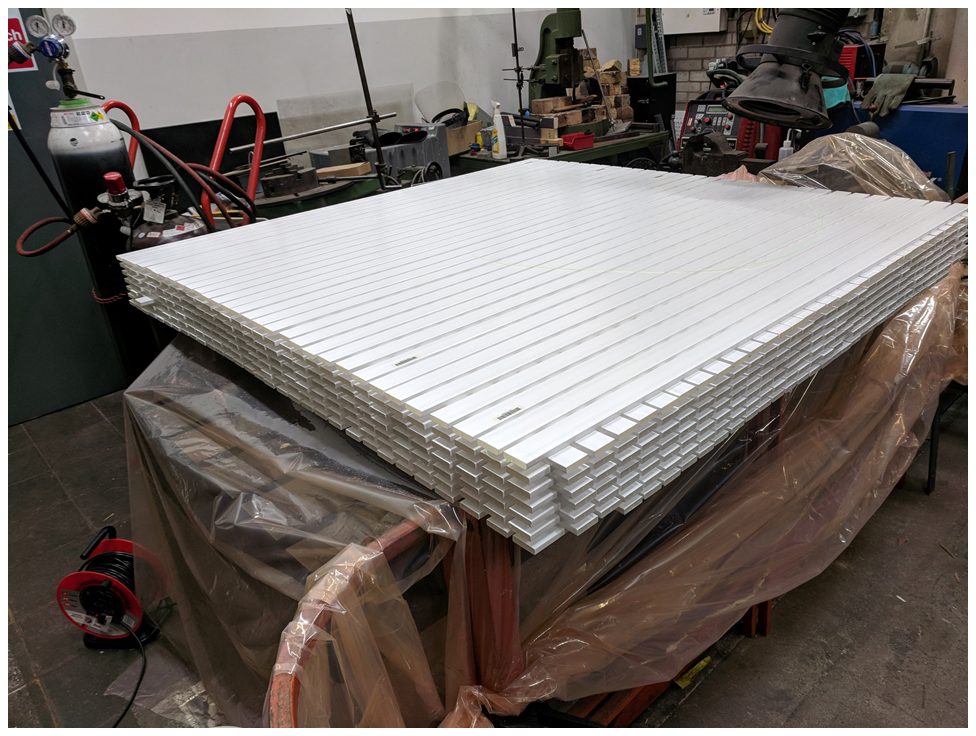
\includegraphics[width=\linewidth]{Chapter3/Figs/Raster/detCon005b_PaintingEnds.png}
  \captionsetup{width=.9\linewidth}
  \caption{}
  \label{subFig:detCon005b_PaintingEnds}
\end{subfigure}
\caption{Scintillator preparation for being placed inside the detector casing. The scintillator is being cut in (a) with arranged for painting the ends in (b).}
\label{fig:detCon_CuttingScint_PaintingEnds}
\end{figure}

\begin{figure}[!h]
\centering
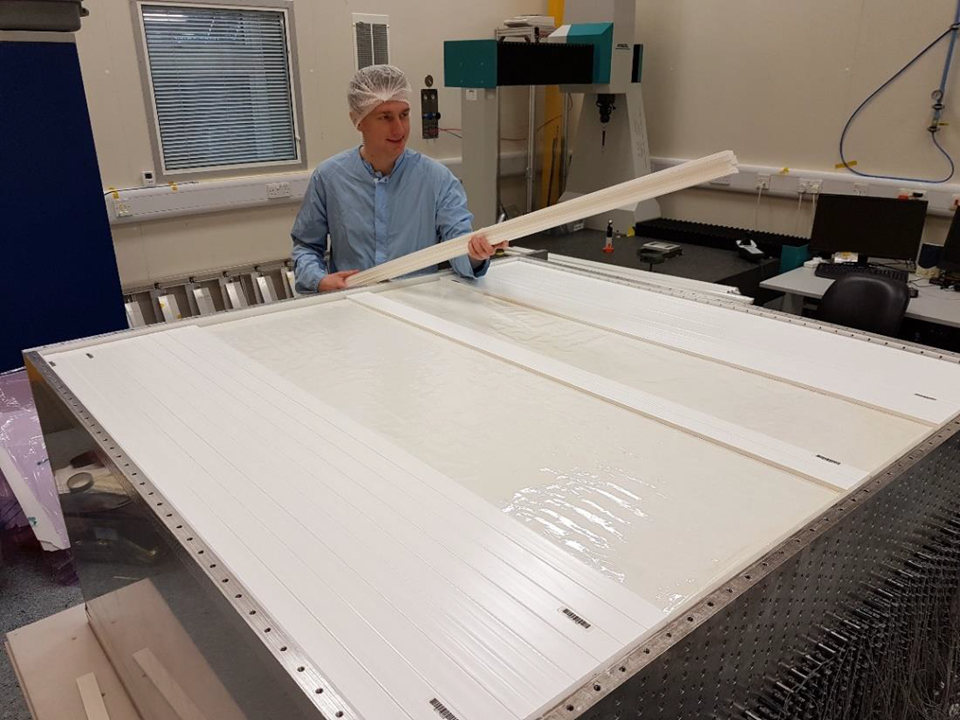
\includegraphics[width=0.7\linewidth]{Chapter3/Figs/Raster/detCon006_RonInCleanRoom.png}
\captionof{figure}{The author (Ronald Collins) in the cleanroom putting scintillator into the detector. The white sheet of Gadolinium Oxide in-between the layers is also visible.} 
\label{fig:detCon006_RonInCleanRoom}
\end{figure}

One of the major improvements made during the upgrade of the VIDARR detector was an increase in cooling. The original detector had much space between the electronic boards and the MPPCs with the electronic boards placed directly on cooling fins (see in figure \ref{fig:detCon002_OldTearAway}). In addition to the cooling fins seen in figure \ref{fig:detCon002_OldTearAway} large radiators have now been added in-between the cooling fins and the MPPCs for each side. These new radiators are comprised of large stainless steel plates which were cut shown in figure \ref{subFig:detCon011b_RadiatorConstruction}. Then copper piping was placed through the sections seen in figure \ref{subFig:detCon012b_RadiatorPiping}. This copper piping will face the MPPCs and the detector scintillator whilst the radiator fins will be attached behind the radiator away from the MPPCs and behind the insulation. As in RMon, the electronic boards will be placed on the fins similar to figure \ref{fig:detCon002_OldTearAway}. This should improve the cooling in the detector significantly as the heat from the electronic boards should be isolated from the scintillator and the MPPCs when compared to the RMon. 

Once the scintillator is in the detector casing several individual components need to be assembled so that the light emitted by the scintillator can then be analysed. A small amount of light emitted by the scintillator upon particle interaction is trapped by the WLS fibres . These fibres are threaded through the centre of the scintillator and capture light and shift it to green light seen in figure \ref{subFig:detCon013b_WlsFibres}. These WLS fibres then have 3D printed connectors glued to the ends of them as seen in figure \ref{subFig:detCon014b_WlsWithEnds}. 3D printing was done as more vacuum moulded parts couldn't be obtained from the original supply chain which RMon used. The 3D printing was done by a Formlabs Form2 resin printer, the components were similar in quality but slightly more brittle and much easier to obtain. Then the MPPCs connectors are 3D printed seen both with the support struts in figure \ref{subFig:detCon015b_3dPrintedHolders} and without in figure \ref{subFig:detCon016b_3dPrintedFreed}. Then the holders for the MPPCs which attach to the Then PCBs which connect the MPPCs to the coaxial cables need to be produced. A sheet of which can be seen in figure \ref{subFig:detCon008b_PlacingPcbs}. These PCBs have to have a coaxial cable connector soldered on to them and pins pushed through them so they can pick up the signals that the MPPCs produce. A finished example of one of these PCBs can be seen in figure \ref{subFig:detCon009b_SoloPcb}. The holders PCBs and MPPCs all fit together as shown in figure \ref{fig:detCon017b_HoldersWithParts}.

\begin{figure}[!h]
\centering
\begin{subfigure}{.5\textwidth}
  \centering
  \includegraphics[width=\linewidth]{Chapter3/Figs/Raster/detCon013b_WlsFibres.png}
  \captionsetup{width=.9\linewidth}
  \caption{}
  \label{subFig:detCon013b_WlsFibres}
\end{subfigure}%
\begin{subfigure}{.5\textwidth}
  \centering
  \includegraphics[width=\linewidth]{Chapter3/Figs/Raster/detCon014b_WlsWithEnds.png}
  \captionsetup{width=.9\linewidth}
  \caption{}
  \label{subFig:detCon014b_WlsWithEnds}
\end{subfigure}
\caption{The WLS fibres will funnel light from the scintillator to the MPPCs. They are assembled on cardboard and have 3d printed ends glued onto them. In (a) the WLS fibres are prepared for their ends by lying on cardboard. In (b) the ends have been glued on.}
\label{fig:detCon_WlsFibres_WlsWithEnds}
\end{figure}

\begin{figure}[!h]
\centering
\begin{subfigure}{.5\textwidth}
  \centering
  \includegraphics[width=\linewidth]{Chapter3/Figs/Raster/detCon015b_3dPrintedHolders.png}
  \captionsetup{width=.9\linewidth}
  \caption{}
  \label{subFig:detCon015b_3dPrintedHolders}
\end{subfigure}%
\begin{subfigure}{.5\textwidth}
  \centering
  \includegraphics[width=\linewidth]{Chapter3/Figs/Raster/detCon016b_3dPrintedFreed.png}
  \captionsetup{width=.9\linewidth}
  \caption{}
  \label{subFig:detCon016b_3dPrintedFreed}
\end{subfigure}
\caption{The holders for the MPPCs and the PCBs. Holders for the additional channels needed to be 3D printed as more from the original supply chain could not be procured. In (a) the holders have the support struts attached and in (b) they have been removed.}
\label{fig:detCon_3dPrintedHolders_3dPrintedFreed}
\end{figure}

\begin{figure}[!h]
\centering
\begin{subfigure}{.5\textwidth}
  \centering
  \includegraphics[width=\linewidth]{Chapter3/Figs/Raster/detCon008b_PlacingPcbs.png}
  \captionsetup{width=.9\linewidth}
  \caption{}
  \label{subFig:detCon008b_PlacingPcbs}
\end{subfigure}%
\begin{subfigure}{.5\textwidth}
  \centering
  \includegraphics[width=\linewidth]{Chapter3/Figs/Raster/detCon009b_SoloPcb.png}
  \captionsetup{width=.9\linewidth}
  \caption{}
  \label{subFig:detCon009b_SoloPcb}
\end{subfigure}
\caption{The assembly of the PCBs which attach to the MPPCs through pins. (a) shows the sheet which had them manufactured and (b) shows a completed component. The connector at the top of the PCBs is where the cables are attached. }
\label{fig:detCon_PlacingPcbs_SoloPcb}
\end{figure}

Each of the coaxial cables that connect the MPPCs to the analogue boards are labelled with heat shrink labels to ensure the labels are secure. The label syntax is side-row-column with the bottom left of each side being the coordinate for (0,0). An example of this syntax would be B-10-37 indicating side B row 10 and column 37. These labels are then slid onto the coaxial cables 8\,cm from the end that connects to the analogue boards. A heat gun is used to shrink the labels onto the coaxial cables. These cables are then connected to the holders where the PCB connector seen in figure \ref{subFig:detCon009b_SoloPcb} connects firmly to the cable. The holder is also put into a sheath so that it is held firmly in place once inside the detector, as seen in figure \ref{fig:detCon023b_HoldersConnectedZoom}.

\begin{figure}[!h]
\centering
\begin{minipage}{.45\textwidth}
  \centering
  \includegraphics[width=\linewidth]{Chapter3/Figs/Raster/detCon017b_HoldersWithParts.png}
  \captionof{figure}{Holder next to MPPC and PCB (Top) and holder with assembled components (Bottom). Note the MPPC in the top right is actually reversed from its correct orientation, the prongs of the MPPC go through the PCB board pins.} 
  \label{fig:detCon017b_HoldersWithParts}
\end{minipage}%
\qquad
\begin{minipage}{.45\textwidth}
  \centering
  \includegraphics[width=\linewidth]{Chapter3/Figs/Raster/detCon023b_HoldersConnectedZoom.png} 
  \captionof{figure}{The holder is connected to a cable and put inside a sheath.}
  \label{fig:detCon023b_HoldersConnectedZoom}
  \vspace*{2.5308cm} %1line = 0.633(3 is recurring)cm  %%% 2lines = 1.2666cm(6 is recurring) %%% 3lines = 1.90cm exactly %%% 4 lines is 2.5308cm exactly  %%% 5lines is 3.1635cm exactly
\end{minipage}
\end{figure}

% \begin{figure}[!h]
% \centering
% \begin{subfigure}{.5\textwidth}
%   \centering
%   \includegraphics[width=\linewidth]{Chapter3/Figs/Raster/detCon018b_HeatLabelsPrinted.png}
%   \captionsetup{width=.9\linewidth}
%   \caption{Heat shrink labels being printed out.}
%   \label{subFig:detCon018b_HeatLabelsPrinted}
% \end{subfigure}%
% \begin{subfigure}{.5\textwidth}
%   \centering
%   \includegraphics[width=\linewidth]{Chapter3/Figs/Raster/detCon019b_CutLabels.png}
%   \captionsetup{width=.9\linewidth}
%   \caption{Individual labels for specific cables.}
%   \label{subFig:detCon019b_CutLabels}
% \end{subfigure}
% \caption{Heat-shrink labels are used to identify cables. Labels are printed out in the form side-Row-Column where the bottom left is (0,0) }
% \label{fig:detCon_HeatLabelsPrinted_CutLabels}
% \end{figure}

% \begin{figure}[!h]
% \centering
% \begin{subfigure}{.5\textwidth}
%   \centering
%   \includegraphics[width=\linewidth]{Chapter3/Figs/Raster/detCon020b_LabelsLoose.png}
%   \captionsetup{width=.9\linewidth}
%   \caption{}
%   \label{subFig:detCon020b_LabelsLoose}
% \end{subfigure}%
% \begin{subfigure}{.5\textwidth}
%   \centering
%   \includegraphics[width=\linewidth]{Chapter3/Figs/Raster/detCon021b_LabelsHeated.png}
%   \captionsetup{width=.9\linewidth}
%   \caption{}
%   \label{subFig:detCon021b_LabelsHeated}
% \end{subfigure}
% \caption{Labels are threaded through at 8\,cm from the end of the cables as seen in (a) then a heat gun is used on the cables to shrink the labels and they are bunched as seen in (b).}
% \label{fig:detCon_LabelsLoose_LabelsHeated}
% \end{figure}



All of the MPPC holders in their sheaths with connected cables are then attached to the WLS fibres and their 3D printed connectors shown in figure \ref{subFig:detCon014b_WlsWithEnds}. There are two distinct sheath types: grey made via injection moulding and orange sheaths which were 3d printed. These sheaths protect the rest of the components and can be seen clearly in figure \ref{fig:detCon_HaningOffRadiator_RadiatorTopDown} as they protrude from the detector casing. The radiator was slowly moved into position as cables were threaded through the insulation as can be seen in figure \ref{subFig:detCon026b_HaningOffRadiator}. Once the radiator was moved into position the space between the radiator and sheaths was checked to ensure that no undue pressure was being applied to the sheaths, which as figure \ref{subFig:detCon028b_RadiatorTopDown} shows there wasn't. Once the radiator was in position the cooling fins were also attached as seen in figure \ref{fig:detCon030b_RadiatorWithFins}. Also in figure \ref{fig:detCon030b_RadiatorWithFins} the x shaped analogue board holders have been attached via thermal paste to the cooling fins. An example of how the analogue boards are attached to the cooling fins can be seen in figure \ref{fig:detCon032_ConnectedBoard}. Which shows how the cables are connected to the analogue boards and aligned through an orange cable comb. 

\begin{figure}[!h]
\centering
\begin{subfigure}{.5\textwidth}
  \centering
  \includegraphics[width=\linewidth]{Chapter3/Figs/Raster/detCon026b_HaningOffRadiator.png}
  \captionsetup{width=.9\linewidth}
  \caption{}
  \label{subFig:detCon026b_HaningOffRadiator}
\end{subfigure}%
\begin{subfigure}{.5\textwidth}
  \centering
  \includegraphics[width=\linewidth]{Chapter3/Figs/Raster/detCon028b_RadiatorTopDown.png}
  \captionsetup{width=.9\linewidth}
  \caption{}
  \label{subFig:detCon028b_RadiatorTopDown}
\end{subfigure}
\caption{As part of the upgrade, the radiators are significantly larger and do not leave much space between the detector and the electronics. In (a) the side A radiator is positioned as the cables are threaded through the insulation on the radiator. In (b) the side A radiator is now in position with all the cables threaded through the insulation.}
\label{fig:detCon_HaningOffRadiator_RadiatorTopDown}
\end{figure}

% \begin{figure}[!h]
% \centering
% \begin{subfigure}{.5\textwidth}
%   \centering
%   \includegraphics[width=\linewidth]{Chapter3/Figs/Raster/detCon029b_coolantFin.png}
%   \captionsetup{width=.9\linewidth}
%   \caption{Board holders that connect the analogue boards to the cooling fins.}
%   \label{subFig:detCon029b_coolantFin}
% \end{subfigure}%
% \begin{subfigure}{.5\textwidth}
%   \centering
%   \includegraphics[width=\linewidth]{Chapter3/Figs/Raster/detCon030b_RadiatorWithFins.png}
%   \captionsetup{width=.9\linewidth}
%   \caption{Cooling fins and board holders attached to the radiator.}
%   \label{subFig:detCon030b_RadiatorWithFins}
% \end{subfigure}
% \caption{The analogue board holders and cooling fins are attached after the cables are threaded through the radiator insulation.}
% \label{fig:detCon_coolantFin_RadiatorWithFins}
% \end{figure}

\begin{figure}[!h]
\centering
\begin{minipage}{.45\textwidth}
  \centering
  \includegraphics[width=\linewidth]{Chapter3/Figs/Raster/detCon030b_RadiatorWithFins.png}
  \captionof{figure}{The radiator on side A with the cooling fins and analogue board holders attached with cables pushed through the insulation and bunched.} 
  \label{fig:detCon030b_RadiatorWithFins}
\end{minipage}%
\qquad
\begin{minipage}{.45\textwidth}
  \centering
  \includegraphics[width=\linewidth]{Chapter3/Figs/Raster/detCon032_ConnectedBoard.png} 
  \captionof{figure}{An analogue board with some of the cables connected to it. A 3D printed cable ``comb'' is used to align the cables.}
  \label{fig:detCon032_ConnectedBoard}
  \vspace{0.6327cm}%1line = 0.6327cm exactly %%% 2lines = 1.2654cm %%% 3lines = 1.8981cm exactly %%% 4 lines is 2.5308cm exactly  %%% 5lines is 3.1635cm exactly
\end{minipage}
\end{figure}

The upgraded container was delivered September 2019 which can be seen in figure  \ref{subFig:detCon037c_ContainerArrives}. But it wasn't until November 2020 that the detector was placed inside its new container (figure \ref{subFig:detCon039b_PutIn2}). The detector upgrade was not complete at this point and currently remains incomplete this is largely due to the COVID-19 pandemic. The upgrade's progress ceased around the same time as the container arrived during September of 2019 as an issue with electronics was discovered. Currently, this remains unresolved. Due to the issues in the electronics supply chain caused by the COVID-19 crisis and the small size of the VIDARR collaboration obtaining replacement electronics has been impossible up to September of 2021. Though in recent months there has been some movement in obtaining the relevant components. 

\begin{figure}[!h]
\centering
\begin{subfigure}{.5\textwidth}
  \centering
  \includegraphics[width=\linewidth]{Chapter3/Figs/Raster/detCon037c_ContainerArrives.png}
  \captionsetup{width=.9\linewidth}
  \caption{}
  \label{subFig:detCon037c_ContainerArrives}
\end{subfigure}%
\begin{subfigure}{.5\textwidth}
  \centering
  \includegraphics[width=\linewidth]{Chapter3/Figs/Raster/detCon039b_PutIn2.png}
  \captionsetup{width=.9\linewidth}
  \caption{}
  \label{subFig:detCon039b_PutIn2}
\end{subfigure}
\caption{The new container arrives in (a) and the partially upgraded detector is deposited inside of it in (b).}
\label{fig:detCon_ContainerArrives_PutIn}
\end{figure}

The upgraded container has much improved airflow when compared to the original including air conditioning and an improved ventilation system. The upgraded container should be able to keep the temperature consistent and thus reduce the uncertainties caused by temperature fluctuations. In addition, there has been a significant improvement to computational power with an upgraded computer rack to read out detector information and a new computer with 64 total threads and 64\,GB of RAM to assist with analysis. Neither of these are currently in the container due to the issues with COVID-19 previously discussed as they are being used to diagnose any issues with the electronics and analyse older data sets.  

% \begin{figure}[!h]
% \centering
% \includegraphics[width=0.7\linewidth]{Chapter3/Figs/Raster/detCon035b_ContainerAirCon.png}
% \captionof{figure}{The new container has air conditioning and an air circulatory system to help keep a consistent temperature.} 
% \label{fig:detCon035b_ContainerAirCon}
% \end{figure}

% \begin{figure}[!h]
% \centering
% \includegraphics[width=0.8\linewidth]{Chapter3/Figs/Raster/detCon037b_ContainerArrives.png}
% \captionof{figure}{The new container arrives at the University of Liverpool.} 
% \label{fig:detCon037b_ContainerArrives}
% \end{figure}

% \begin{figure}[!h]
% \centering
% \includegraphics[width=0.8\linewidth]{Chapter3/Figs/Raster/detCon039_PutIn2.png}
% \captionof{figure}{The new detector being placed in the new container. (The upgrade was only partially completed at this time)} 
% \label{fig:detCon039_PutIn2}
% \end{figure}

% \begin{figure}[!h]
% \centering
% \includegraphics[width=0.7\linewidth]{Chapter3/Figs/Raster/detCon042b_Rack1.png}
% \captionof{figure}{The computer rack for the upgraded detector from the back (left) and front (right).} 
% \label{fig:detCon042b_Rack1}
% \end{figure}

% \begin{figure}[!h]
% \centering
% \includegraphics[width=0.8\linewidth]{Chapter3/Figs/Raster/detCon044_NewComputer.png}
% \captionof{figure}{The new computer for the upgraded detector. It has two 32 core CPUs and 64\,Gb of Ram.} 
% \label{fig:detCon044_NewComputer}
% \end{figure}

% \begin{figure}[!h]
% \centering
% \includegraphics[width=0.7\linewidth]{Chapter3/Figs/Raster/detCon045b_PowerCabels1.png}
% \captionof{figure}{Power cables for the analogue boards that will attach to the central bus bars. \hl{may need to add some finer details remember to check with Carl}} 
% \label{fig:detCon045b_PowerCabels1}
% \end{figure}
%*******************************************************************************
%****************************** Fourth Chapter *********************************
%*******************************************************************************


\chapter{GEANT4 Simulation}\label{chp:geant4Simulation}
\ifpdf
    \graphicspath{{Chapter4/Figs/Raster/}{Chapter4/Figs/PDF/}{Chapter4/Figs/}}
\else
    \graphicspath{{Chapter4/Figs/Vector/}{Chapter4/Figs/}}
\fi

\section{GEANT4 Overview}\label{sec:geant4Simulation_g4Overview}
The VIDARR detector is also represented in a GEANT4 simulation which is a provident physics simulation package. According to the GEANT4 collaboration GEANT4 ``covers a comprehensive range including electromagnetic, hadronic and optical processes and a large set of long-lived particles materials and elements over a wide energy range starting in some cases from 250\,eV and extending in others to the TeV range'' \cite{Agostinelli:2002hh}. Considering that the energy range for inverse $\beta$ decay is 2\,MeV-8\,MeV \cite{Mueller_2011} this simulation package appears to meet the needs of the VIDARR collaboration. However whilst the simulation of the resulting positrons is reasonably simplistic the simulation of the neutrons is more challenging due to the difficulty in simulating the Gadolinium cascade. 

\section{Modelling The VIDARR Upgrade}

\begin{figure}[htbp]
 \centering
 \includegraphics[width=0.7\linewidth]{Chapter4/Figs/Raster/containment_Energy.png}
 \captionof{figure}{Quality of the containment of event energy in the 1862 bars detector and the 2660 bars detector where the containment is defined as the percentage of $\gamma$ cascade reconstructed energy compared to the $\gamma$ cascade generated energy.} %~can be used as a kind of place holder in latex
 \label{fig:containment_comparison}
\end{figure} 

\section{Gadolinium Cascade}\label{sec:geant4Simulation_gdCascade}
The Gadolinium cascade is difficult to measure and accurately simulate for for two main reasons. The first is that the gadolinium nuclei that have good neutron capture are isotopes $^{155}$Gd and $^{157}$Gd which have 155 and 157 nucleons respectively. Both of these nuclei are large and as such it is difficult to accurately model the individual interactions between each of the nucleons. So, there is no agreed upon model at present for the absorption and emission of the 8\,MeV $\gamma$ cascade. The second issue is that the high energy $\gamma$ rays emitted by the cascade are very difficult to contain. Therefore, getting accurate measurements and energy efficiencies for the cascade is also very difficult. These two problems compound one another it is difficult to measure the cascade so it is difficult to model which, in turn, makes it difficult to know the energies expected to be emitted by the nuclei. Further issues are caused by highly penetrative making efficiency estimates even less accurate. \hl{(No references... whilst this is all reasonably straight forward some more concrete numbers and figures would be nice...)}. Gadolinium is used because of its high efficiency (10$\%$ - 40$\%$) compared to other neutron capturing materials such as $^6$Li which only has about $1\%$ \cite{Abdushukurov_2010}. 
\\\\The simulation has several distinct modes: cosmic $\mu$, noise, and inverse $\beta$ decay. The cosmic mode has a realistic distribution \hl{what paper did Matt Murdock use to form the realistic distribution?} and a cosmic hemisphere distribution. The cosmic hemisphere distribution is used to check that the analysis chain is functioning as expected and for testing simulated reactor shadows. In all other cases the realistic cosmic distribution is used when simulating cosmic $mu$s. The noise distributions are random uniform distributions from 0 - 10\,MeV simulating which cover $p$,$\bar{p}$,$\pi^+$,$\pi^-$,$e^-$,$e^+$, $\alpha$,$\bar{\alpha}$,$n$. The IBD simulation is done by simulating a positron between 0 - 10\,MeV and then simulating at $\sim$ 10 $\mu$s later a neutron. \hl{Timing plot required!}. The range 0 - 10\,MeV is used instead of 2 - 8\,MeV to allow the testing of edge cases and for better fitting and or particle identification later down the road. \hl{need figures for both cosmic and ibd, this requires access to OLL however...}.
\section{Modelling Attenuation}\label{sec:geant4Simulation_ModellingAttenuation}
In order to characterise the physical effects of the detector at test stand was set up by fellow collaborator George Holt. This test stand contained a single plastic scintillating bar where a caesium 137 source was placed at 11 intervals across the bar from which attenuation of the 662\,KeV peak could then be measured. This is then shown in figure \ref{fig:attenuationPlot} this exponential decay is then put into the simulation so that the amount of light produced is more physical. 
\begin{figure}[htbp]
 \centering
 \includegraphics[width=1.0\linewidth]{result_from_attnPlotter.png} 
 \captionof{figure}{The attenuation plot for test stand produced by George Holt. The attenuation length is 580 $\pm$ 60 \hl{units!}} 
 \label{fig:attenuationPlot}
\end{figure}

\section{Modelling Dark Noise}\label{sec:geant4Simulation_ModellingDarkNoise}
Another data driven physical effect modelled in the simulation is the dark noise. Depending on the temperature of the room the electronics in an MPPC will give signals that are non-physical. The dark noise was measured at room temperature by George Holt over a 12 hour period the results in figure \ref{fig:pureDarkNoise} show peaks in units of photo-electrons (PE) with peaks for 1\,PE, 2\,PE and 3\,PE being clearly visible. The MPPC was put inside a container where no light would reach the sensor. 
\begin{figure}[htbp]
 \centering
 \includegraphics[width=0.8\linewidth]{pureDarkNoise_output.png}
 \captionof{figure}{Dark Noise from the MPPC taken over a period of $\sim$ 12\,hrs. The PE peaks for 1\,PE 2\,PE and 3\,PE can be seen at 4.1\,mv, 8.2\,mv and 12.3\,mv respectively. } 
 \label{fig:pureDarkNoise}
\end{figure}

The dark noise has two distinct components, the peaks and the background surrounding the peaks. The background surrounding the peaks can be modelled using an exponential fit and is done so in figure \ref{subFig:expFitOfDark}. The pedestal peak is also removed and then the exponential is used past 13.7\,mV which can be seen in figure \ref{subFig:fittedDarkNoise}. 
\begin{figure}[htbp]
\centering
\begin{subfigure}{.5\textwidth}
  \centering
  \includegraphics[width=\linewidth]{fit_of_dark_noise.png}
  \captionsetup{width=.9\linewidth}
  \caption{Fit of exponential function using TFit to fit the after-pulsing of the MPPCs}
  \label{subFig:expFitOfDark}
\end{subfigure}%
\begin{subfigure}{.5\textwidth}
  \centering
  \includegraphics[width=\linewidth]{fittedDarkNoise_output.png}
  \captionsetup{width=.9\linewidth}
  \caption{Fitted exponential past 13.7\,mv once the number of events dropped below 10.}
  \label{subFig:fittedDarkNoise}
\end{subfigure}
\caption{Dark Noise from the MPPC taken over a period of $\sim$ 12\,hrs with an exponential fitted, with a $\chi ^2$ /DOF = 159.748}
\label{fig:fitting_of_non_peak_dark_noise}
\end{figure}

The results from \ref{fig:fitting_of_non_peak_dark_noise} can then be used to construct a cumulative distribution seen in figure \ref{fig:cumulative_prob_dark}, this cumulative distribution is what is used by the simulation in order to visnstruct the dark noise distribution. During the simulation a random dice is thrown that probability is then converted back into a dark noise value which is then assigned to a random bar in the detector. Values past 13.7\,mV use the exponential fit.
\begin{figure}[htbp]
 \centering
 \includegraphics[width=0.8\linewidth]{cumulative_prob_dark_noise.png}
 \captionof{figure}{cumulative probability of the dark noise, which is converted to a table and then searched using the golden section search} 
 \label{fig:cumulative_prob_dark}
\end{figure}
\hl{would be really nice if I could produce a histo of the simulated dark noise and quantify what that looks like and how much we're expecting when we deploy}

\section{Modelling Light Emission}\label{sec:geant4Simulation_ModellingLightEmission}
In order to measure light for a given amount of scintillating material we need to consider several factors. For organic scintillators the type of particle has a significant effect on the absolute light yield. The response of organic scintillators to charged particles can best be described by a relation between $dL/dx$ the fluorescent energy emitted per unit path length and $dE/dx$ the specific energy loss for the charged particle.  A widely used relation first suggested by Birks \cite{birks_1964} is based on the assumption that a high intonation density along the track of the particle leads to quenching from damaged molecules and a lowering of the scintillation efficiency. If we assume that the density of damage molecules along the wake of the particle is directly proportional to the ionisation density we can represent their density by $B(dE/dx)$ where $B$ is a proportionality constant. Birks assumes that some fraction $k$ of theses will lead to quenching\cite{knoll_2010}. A further assumption is that in absence of quenching the light yield is proportional to energy loss shown in equation \ref{equ:light_yield_proportional}. $S$ is the normal scintillation efficiency. To account for the probability of quenching birks then writes equation \ref{equ:Birks_formula}. Equation \ref{equ:Birks_formula} is commonly referred to as Birks formula. As a practical matter the product $kB$ is treated as an adjustable parameter to fit experimental data for a specific scintillator whereas $S$ is particle specific which provides absolute normalisation \cite{knoll_2010}.  
\begin{equation}
\frac{dL}{dx} = S\frac{dE}{dx}
\label{equ:light_yield_proportional}
\end{equation}
\begin{equation}
\frac{dL}{dx} = \frac{S\frac{dE}{dx}}{1 + kB \frac{dE}{dx}}
\label{equ:Birks_formula}
\end{equation}
\\\\In this model molecules in the ionisation column are labelled ``damaged'' and ``undamaged'' for convenience where ``damaged'' molecules are those which dissipate ionisation energy nonradiatively (quenching) and so lower scintillation efficiency\cite{craun_1970} \cite{knoll_2010}. ``Damaged'' molecules occupy highly ionised or excited states, they de-excite quickly ($<$ 1 ns) to the ``undamaged'' condition \cite{craun_1970}. Some permanent damage will occur and does contribute to long term degradation of the scintillator but is not relevant for quenching\cite{craun_1970}. From this B is the ratio of ``damaged''/``undamaged'' molecules and k is the relative probability of quenching. kB is treated as a single adjustable parameter as there is no way to measure k or B separately \cite{craun_1970} \cite{knoll_2010}. Where kB is scintillator dependant only and will be refereed to as a single entity as Birk's constant. The response for electrons above $\sim$ 125\,keV is linear \cite{craun_1970}. This is also seen in Birk's law which also becomes linear for fast electrons \cite{knoll_2010}. This is important for modelling electrons. 
\section{MINERvA Birk's Constant}\label{sec:geant4Simulation_MINERvABirksConstant}
In equation \ref{equ:Birks_formula} the parameters $kB$ and $S$ are empirically determined. $S$ is a normalisation parameter that is particle dependent and kB is the birks constant for the scintillator and is particle independent. The MINERvA collaboration \cite{aliaga_2015} also uses the same scintillator as the VIDARR detector \cite{aliaga_2014}, the collaboration determined the value of the of kB to be 0.0905 $\pm$ 0.015\,mm/MeV at best fit. This Birks parameter was obtained by using GEANT4 MC data, which is the same approach by which VIDARR has obtained its birks parameter.
Both the VIDARR and MINERvA approach use the Geant4 bertini cascade model when attempting to measure the \\\\Birks parameter $kB$ \cite{Heikkinen_2003}. In addition both use the QGSP physics list which applies the quark gluon string model when simulating particles \cite{Patrick_2018}. The steps have to remain course in Geant4 otherwise the $kB$ parameter changes  \cite{aliaga_2015}. This is why the EMY physics lists were not used, even though they simulate smaller steps and so would potentially simulate stopping better. Then energy range for the MINERvA signal is of order $\sim$ 1\,GeV, whereas the energy range for VIDARR's signal is 0-10\,MeV. However a major source of noise for VIDARR are cosmic muons which have energies $\sim$ 1\,GeV and protons with energies between 0-10\,MeV as a result of fast neutrons. Using the minerva data requires going to higher energies (lower $dE/dx$) in order to ensure similar results in the $dL/dx$ fit.  
\\\\The results of the MINERvA Birks law investigation concluded that a birks constant of 0.0905 $\pm$ 0.015\,mm/MeV was the most accurate value for the scintillator \cite{aliaga_2015}. Whilst the MINERvA experiment measures protons with an energy range of 0\,MeV-500\,MeV and the particles of VIDARR's interest are $\overline{\nu_{e}}$s with energy range between 0\,MeV-10\,MeV the Birk's constant is the same regardless. This is because the Birk's law is a representation of the scintillator itself and therefore is not particle or energy dependent, the amount of saturation in the scintillator that the Birks constant represents is constant in all cases. 

\section{Loss of Deposited Energy due to Quenching}\label{sec:geant4Simulation_quenchingLoss}
\hl{Very Important!: This work is currently not replicable, the collection of scripts is on my hepstore somewhere and needs to be backed up and put onto git as soon as possible!}
\\\\The effect of quenching varies greatly depending on the particle it is a function of both energy and mass. By considering three example particles and their corresponding anti-particles the scale of quenching can be observed. The first particle to consider would be electrons as they are one of the most common sources of noise and have a large charge to mass ratio when compared to other particles that could be potential background for this experiment. The level of quenching for electrons and positrons is very minimal which can be seen in figure \ref{fig:electron_positron_quenched_and_not}. This was simulated using a ``slab'' of material, figure \ref{fig:electrons_viewed_in_slab}, instead of using a bar or a full detector this was done to ensure that all of the energy was kept inside the plastic scintillator so that the full energy loss due to quenching could be measured. 

\begin{figure}[htbp]
\centering
\begin{subfigure}{.5\textwidth}
  \centering
  \includegraphics[width=\linewidth]{quench_eng_LinElectrons.png}
  \captionsetup{width=.9\linewidth}
  \caption{Visible electron energy deposition with and without quenching}
  \label{subFig:electron_quenched_and_not}
\end{subfigure}%
\begin{subfigure}{.5\textwidth}
  \centering
  \includegraphics[width=\linewidth]{quench_eng_LinPositrons.png}
  \captionsetup{width=.9\linewidth}
  \caption{Visible positron energy deposition with and without quenching}
  \label{subFig:positron_quenched_and_not}
\end{subfigure}
\caption{Electrons and positrons visible energy with and without quenching in a ``slab'' of material}
\label{fig:electron_positron_quenched_and_not}
\end{figure}

\begin{figure}[htbp]
\centering
\begin{subfigure}{.5\textwidth}
  \centering
  \includegraphics[width=\linewidth]{e-_10MeV_Length_on_view.png}
  \captionsetup{width=.9\linewidth}
  \caption{electrons side on view in ``slab''}
  \label{subFig:electron_side_slab}
\end{subfigure}%
\begin{subfigure}{.5\textwidth}
  \centering
  \includegraphics[width=\linewidth]{e-_10MeV_side_on_view.png}
  \captionsetup{width=.9\linewidth}
  \caption{electron length on view in ``slab''}
  \label{subFig:electron_length_slab}
\end{subfigure}
\caption{Electron side and length on view in ``slab'' of material, the electrons are not leaving the material.}
\label{fig:electrons_viewed_in_slab}
\end{figure}

The effect of quenching on protons is much more significant than for electrons, this is because the charge for protons is equal and opposite for electrons but the mass is $\sim$ 2000 times greater than for electrons. This results in a large amount of energy no longer being deposited in the scintillator which can be seen in figure \ref{fig:proton_Apronton_quenched_and_not} which shows both the energy deposition of protons and anti-protons. In figures \ref{subFig:proton_quenched_and_not}, \ref{subFig:Aproton_quenched_and_not} the energy deposition is linear for protons and anti-protons without quenching this suggests that the majority of the energy lost is lost via quenching. For $\alpha$ particles the effect is even more significant $\alpha$ particles which are 4 times more massive than protons but have twice the charge. The effect of quenching is $\sim$ 4 times greater for $\alpha$ particles than for protons which can be seen when comparing the energy deposited in the slab for figures \ref{fig:proton_Apronton_quenched_and_not} and \ref{fig:alpha_Aalpha_quenched_and_not}. 

\begin{figure}[htbp]
\centering
\begin{subfigure}{.5\textwidth}
  \centering
  \includegraphics[width=\linewidth]{quench_eng_protons.png}
  \captionsetup{width=.9\linewidth}
  \caption{Visible proton energy deposition with and without quenching}
  \label{subFig:proton_quenched_and_not}
\end{subfigure}%
\begin{subfigure}{.5\textwidth}
  \centering
  \includegraphics[width=\linewidth]{quench_eng_Aprotons.png}
  \captionsetup{width=.9\linewidth}
  \caption{Visible anti-proton energy deposition with and without quenching}
  \label{subFig:Aproton_quenched_and_not}
\end{subfigure}
\caption{protons and anti-protons visible energy with and without quenching in a ``slab'' of material}
\label{fig:proton_Apronton_quenched_and_not}
\end{figure}

\begin{figure}[htbp]
\centering
\begin{subfigure}{.5\textwidth}
  \centering
  \includegraphics[width=\linewidth]{quench_eng_Alpha.png}
  \captionsetup{width=.9\linewidth}
  \caption{Visible alpha particle energy deposition with and without quenching}
  \label{subFig:alpha_quenched_and_not}
\end{subfigure}%
\begin{subfigure}{.5\textwidth}
  \centering
  \includegraphics[width=\linewidth]{quench_eng_AAlpha.png}
  \captionsetup{width=.9\linewidth}
  \caption{Visible anti-alpha particle energy deposition with and without quenching}
  \label{subFig:Aalpha_quenched_and_not}
\end{subfigure}
\caption{alpha and anti-alpha particles visible energy with and without quenching in a ``slab'' of material}
\label{fig:alpha_Aalpha_quenched_and_not}
\end{figure}

\section{Monte Carlo Modelling of Birks Law}\label{sec:geant4Simulation_MonteCarloBirksLaw}
\hl{Very Important!: This work is currently not replicable, the collection of scripts is on my hepstore somewhere and needs to be backed up and put onto git as soon as possible!}
\\\\The photon model in Geant4 is computationally expensive as the simulation toolkit simulates optical photon tracks at every energy deposition for a given amount of energy. With a scintillation yield of $10^5$\,ph/MeV as in this simulation the slowdown observed at higher energies is extreme. This slowdown can be somewhat alleviated by counting the number of photons and then killing the optical photon tracks, as it is the number of photons produced that determines quenching, but even this is still computationally expensive. So whilst the count and kill method was used for determining Birk's law, once the light was characterised the count and kill method was abandoned due to its high computational load.
\\\\In order to accurately quantify the response of Birks law Monte Carlo modelling was used in Geant4. This was done so that the value of $S$ in equation \ref{equ:Birks_formula} could be found for each particle. The Geant4 physics list of QGSP\_\_BERT\_\_HP allows for good repdouction of Birk's law \cite{Patrick_2018},\cite{aliaga_2015}. However, two new models of the scintillator were required in order to accurately quantify the effects of the Birk's constant, both of them required the removal of all wavelength shifting fibres and MPPCs and so are just scintillator. The first model was a ``slice model'' that was 1\,mm thick and had a cross section of 0.2\,m by 0.2\,m, this allowed for the approximations $dL/dx \approx \Delta L / \Delta x$ and $dE/dx \approx \Delta E / \Delta x$ to be used. The second model was a ``slab'' model (figure \ref{fig:electrons_viewed_in_slab}) that was 2\,m thick and had a cross section of 0.2\,m by 0.2\,m, this model was used for determining how effective the Birk's approximation was. Both models had particle energy ranges of 0\,MeV-100\,MeV.
The ``slice'' model was used to determine the $S$ values for every particle in equation \ref{equ:Birks_formula}, once those had been obtained the $kB$ value of 0.0905 $\pm$ 0.015\,mm/MeV obtained from MINERvA was also used. By using the approximations $dL/dx \approx \Delta L / \Delta x$ and $dE/dx \approx \Delta E / \Delta x$ and using $\Delta L = L_{\textrm{end}} - L_{\textrm{start}} $ where in the simulation it is known the light at the start of the step $L_{\textrm{start}} = 0$ and $L_{\textrm{end}}$ is the Light at the end of each Geant4 step allows for equation \ref{equ:light_produced} to be created. Using equation \ref{equ:light_produced} the light yeild can now be calculated, the following particles were simulated: $e^-$,$e^+$,$p$,$\overline{p}$,$\pi^+$,$\pi^-$,$\mu^-$,$\mu^+$,$\alpha$,$\overline{\alpha}$. 
\begin{equation}
L_{\textrm{end}}\approx \Delta x \left(\frac{S\frac{\Delta E}{\Delta x}}{1 + kB \frac{\Delta E}{\Delta x}}\right) 
\label{equ:light_produced}
\end{equation}
The approximations that the Birks law predicts for $p$,$\overline{p}$,$\pi^+$,$\pi^-$,$\mu^-$,$\mu^+$,$\alpha$,$\overline{\alpha}$ are very close to the model of light that Geant4 predicts. The deviation from Geant4 is at the worst at 100\,MeV where there is a deviation of $\sim$ $3\%$ in light output between Geant4 and the Birks approximation of protons and anti-protons seen in figure \ref{fig:proton_aproton_light} with \ref{subFig:proton_light} representing protons and \ref{subFig:aproton_light} representing anti-protons. The Brik's approximation proves to be a closer fit to the data than the simulated light fit which is a square function ($L = aE^2 + bE+ c$). \hl{IMPORTANT NOTE TO SELF: The chisq/ndf are awful in both cases, but there must be a way to show one is better than the other.}
\begin{figure}[htbp]
\centering
\begin{subfigure}{.5\textwidth}
  \centering
  \includegraphics[width=\linewidth]{light_of_protons0-100mev.png}
  \captionsetup{width=.9\linewidth}
  \caption{proton light produced by Geant4 compared to the Birks approximation of that light, the simulated light fit is the square funciton $L = aE^2 + bE+ c$ and is fit to the Geant4 simulated light}
  \label{subFig:proton_light}
\end{subfigure}%
\begin{subfigure}{.5\textwidth}
  \centering
  \includegraphics[width=\linewidth]{light_of_Aprotons0-100mev.png}
  \captionsetup{width=.9\linewidth}
  \caption{anti-proton light produced by Geant4 compared to the Birks approximation of that light, the simulated light fit is the square funciton $L = aE^2 + bE+ c$ and is fit to the Geant4 simulated light}
  \label{subFig:aproton_light}
\end{subfigure}
\caption{proton and anti-proton light output compared to the birks approximation and a square fit to the light out put in Geant4}
\label{fig:proton_aproton_light}
\end{figure}
However the light yield for electrons and positrons seen in figure \ref{fig:electron_positron_light} varies more significantly. A variation of $\sim$ 15\,\% is seen in the electrons, figure \ref{subFig:electron_light}, and a variation and a variation of $\sim$ 20\,\% is seen in positrons, figure \ref{subFig:positron_light} at maximum energy values. In figure \ref{fig:electron_positron_light}, the simulated light fit, which is a square fit to the data in the form $L = aE^2 + bE+ c$ fits the data far closer. Figure \ref{fig:square_electron_positron_light} shows this approximation inputted instead, there is a slight variation between the simulated light fit and the square approx. seen in figures \ref{subFig:square_electron_light} and \ref{subFig:square_positron_light}. This is because the simulated light fit is fitted to the whole light distribution whereas the light of the square approximation is produced per Geant4 step. Despite this, the square approximation of light for electrons ($L = 0.9347E^2 + 10340E - 0.1000$) had a variation of 0.7\,\% at maximum energy and the square approximation of the light for the positrons ($L = 0.9716E^2 + 10350E -0.1000$) had a variation of 0.3\,\% at maximum energy. 
\begin{figure}[htbp]
\centering
\begin{subfigure}{.5\textwidth}
  \centering
  \includegraphics[width=\linewidth]{light_of_electrons0-100mev.png}
  \captionsetup{width=.9\linewidth}
  \caption{Electron light produced by Geant4 compared to the Birks approximation of that light, the simulated light fit is the square funciton $L = aE^2 + bE+ c$ and is fit to the Geant4 simulated light}
  \label{subFig:electron_light}
\end{subfigure}%
\begin{subfigure}{.5\textwidth}
  \centering
  \includegraphics[width=\linewidth]{light_of_positrons0-100mev.png}
  \captionsetup{width=.9\linewidth}
  \caption{Positron light produced by Geant4 compared to the Birks approximation of that light, the simulated light fit is the square funciton $L = aE^2 + bE+ c$ and is fit to the Geant4 simulated light}
  \label{subFig:positron_light}
\end{subfigure}
\caption{Electron, Positron light output compared to the birks approximation and a square fit to the light out put in Geant4}
\label{fig:electron_positron_light}
\end{figure}
\begin{figure}[htbp]
\centering
\begin{subfigure}{.5\textwidth}
  \centering
  \includegraphics[width=\linewidth]{light_of_electronsLin0-100mev.png}
  \captionsetup{width=.9\linewidth}
  \caption{Electron light simulated by Geant4 compared to the square approximation $L = aE^2 + bE+ c$ }
  \label{subFig:square_electron_light}
\end{subfigure}%
\begin{subfigure}{.5\textwidth}
  \centering
  \includegraphics[width=\linewidth]{light_of_positronsLin0-100mev.png}
  \captionsetup{width=.9\linewidth}
  \caption{Positron light simulated by Geant4 compared to the square approximation $L = aE^2 + bE+ c$}
  \label{subFig:square_positron_light}
\end{subfigure}
\caption{Electron and positron light output from simulation compared to a Geant4 step square approximation}
\label{fig:square_electron_positron_light}
\end{figure}
The conversion for light into energy for electrons in figure \ref{subFig:square_electron_light} is defined by equation \ref{equ:MeV_electron_equivalent_square}. The light of an electron is the highest amount of light per MeV that a particle can deposit this MeV electron equivalent (MeVee) is a special nomenclature used to describe the absolute light yeild \cite{knoll_2010}. As the squared term $ << $ the linear term, the squared term is ignored for the purposes of light conversion, producing equation \ref{equ:MeV_electron_equivalent_linear}. By rearranging equation \ref{equ:MeV_electron_equivalent_linear} for energy production we then get equation \ref{equ:MeV_electron_equivalent_light} which allows for the conversion from the Birks approximation of light into the energy or the square approximation of light into energy for the electrons and positrons. With equation \ref{equ:MeV_electron_equivalent_light} it is possible to show the energy loss due to quenching, once the L in equation \ref{equ:MeV_electron_equivalent_light} is substituted with the light at the end of the Geant4 step shown in equation \ref{equ:light_produced}. \hl{IMPORTANT NOTE TO SELF: Again chisqs for this are very very poor, but I don't know how to make better, must return to this at a later date!} 
\begin{equation}
L = 0.9347E^2 + 10340E - 0.1000
\label{equ:MeV_electron_equivalent_square}
\end{equation}
\begin{equation}
L = 10340E - 0.1000
\label{equ:MeV_electron_equivalent_linear}
\end{equation}
\begin{equation}
E = \frac{L +0.1000}{10340} 
\label{equ:MeV_electron_equivalent_light}
\end{equation}

\section{Counting Statistics} \label{sec:geant4Simulation_countingStats}
When a particle passes through the scintillating plastic it produces photons as it interacts. These photons then travel through the bar until they meet the wavelength shifting fibres (wls). The photons then travel down the wls until they encounter the MPPC  this signal is them amplified by the MPPC producing a signal of 4.2\,mV which is equivalent for one photon see figure \ref{fig:pureDarkNoise} which is called a photo-electron equivalent (PE). So for n number of photo-electron equivalents there will be a Poisson distribution (equation \ref{equ:possionProb}) associated with it due to counting statistics. This only holds true if there is a small probability of a given outcome which is true for this case. For this distribution $pn = \overline{x}$ where $\overline{x}$ is the expectation value, substituting this into equation \ref{equ:possionProb} we get equation \ref{equ:possionExpectation} \cite{knoll_2010}.
\begin{equation}
P(x) = \frac{(pn)^x e^{-pn}}{x!}  
\label{equ:possionProb}
\end{equation}

\begin{equation}
P(x) = \frac{(\overline{x})^x e^{-\overline{x}}}{x!}  
\label{equ:possionExpectation}
\end{equation}

Further the variance of this model can thus be explained using equation  \ref{equ:possionVar} which also gives $\sigma^2 = \overline{x}$ and thus gives a standard deviation of $\sigma = \sqrt{\overline{x}}$ \cite{knoll_2010}. This definition is also of the standard deviation is also true for the Gaussian distribution. The Gaussian distribution which uses this standard deviation can be seen in equation \ref{equ:guassianExpectation}. When n is high enough the Poisson distribution will approximate to a Gaussian distribution this is useful when simulating light counting statistics because a Gaussian distribution is much less computationally intensive as there is no factorial. The point where Gaussian is used instead of Poisson in the simulation is at a value of 10 photons seen in figure \ref{fig:CoutingStats10}, this is when 99.9\,\% of the distribution having 2 photons which is the limit for hits to be considered. 

\begin{equation}
\sigma ^2 \equiv \sum_{x=0}^{n} (x-\overline{x})^2 P(x) = pn = \overline{x} 
\label{equ:possionVar}
\end{equation}

\begin{equation}
P(x) = \frac{1}{\sigma \sqrt[]{2 \pi}} \exp \left(-\frac{1}{2}\left(\frac{x-\overline{x}}{\sigma}\right)^{2}\right)
\label{equ:guassianExpectation}
\end{equation}

\begin{figure}[htbp]
 \centering
 \includegraphics[width=0.8\linewidth]{countingStats10.png}
 \captionof{figure}{Counting statistics for poission and normal distribution for an expectation value of 10 photons the normal distribution is used past when the expectation value is 10 photons or higher to save on computational load.} 
 \label{fig:CoutingStats10}
\end{figure}

\section{Simulated Results With Physical and Electronic Effects}\label{sec:geant4Simulation_resultsPhysicalElectronics}
The impact of physical and electronic effects on simulated data is quite significant especially for heavier particles such as protons and $\alpha$s. The heaviest particle we expect to see in statistically significant quantities is the $\alpha$ in order to show the maximum difference between generated and more realistic simulation generated $\alpha$ particles are used for this section. 
\\\\If these effects are left out of the simulation then the results look nonphysical in figure \ref{fig:alpha_summed_vs_truth} the summed energy inside the detector is equal to the truth energy in most cases. The only events which do not have all the energy summed in the detector are those which were generated near the edges of the bar, these events are absorbed by the TiO$_2$ coating and so deposit less energy in the detector. The modelling of quenching (see section \ref{sec:geant4Simulation_MonteCarloBirksLaw}) and attenuation (see figure \ref{fig:attenuationPlot}) therefore cause a large decrease in the summed energy inside the detector seen in figure \ref{fig:alphaVisVsTruthZoom}. This version of the data can be seen as what an idealistic version of the VIDARR detector could produce. The detector response is longer linear due to he effects described by Birk's Law. 
\begin{figure}[htbp]
 \centering
 \includegraphics[width=0.7\linewidth]{truth_vs_summed_alpha.png}
 \captionof{figure}{The energy deposited in a simulated detector by $\alpha$ particles without physical and electronic effects taken into account, this is the maximum possible energy that can be deposited.} 
 \label{fig:alpha_summed_vs_truth}
\end{figure}
\begin{figure}[htbp]
 \centering
 \includegraphics[width=0.7\linewidth]{Chapter4/Figs/Raster/truth_vs_visSummed_alpha_zoom.png}
 \captionof{figure}{The energy deposited in a simulated detector by $\alpha$ particles with only the physical effects of quenching and attenuation taken into account. The detector effects of dark noise and counting statistics are not taken into account} 
 \label{fig:alphaVisVsTruthZoom}
\end{figure}


Finally the effects caused by the electronics and the counting statistics (figure \ref{fig:CoutingStats10}) gives the simulated distribution a more realistic shape. The results for this can be seen in figure \ref{fig:alphaRecoVsTruthZoom}. With the data driven effects taken into account the simulation should give a more realistic result. Unfortunately due to the outbreak of Covid-19 the detector construction was delayed and so the accuracy of this simulation can only be benched marked against the individual components rather than the detector as a whole. 
\begin{figure}[htbp]
 \centering
 \includegraphics[width=0.7\linewidth]{Chapter4/Figs/Raster/truth_vs_recoSummed_alpha_zoom.png}
 \captionof{figure}{The energy deposited in a simulated detector by $\alpha$ particles with physical effects of quenching and attenuation taken into account as well as the detector effects of dark noise and counting statistics.} 
 \label{fig:alphaRecoVsTruthZoom}
\end{figure}

\section{Modelling Gadolinium}\label{sec:geant4Simulation_modellingGadolinium}
Gadolinium is useful for measuring inverse $\beta$ decay as when the neutron is given off and subsequently absorbed by the layer of gadolinium in between the layers of scintillating plastic in the VIDARR detector a delayed 8\,MeV $\gamma$ cascade is released. This is the trigger signal for the VIDARR detector. After the cascade has been triggered the detector looks backwards in time to determine the positron cluster. 
\\\\Gadolinium has two models in Geant 4 the photon evaporation model seen in \ref{subFig:differentGeant4Models_photonEvaporationGd} and the final state model seen in  \ref{subFig:differentGeant4Models_finalStateGd}. These two models have different strengths and weaknesses the photon evaporation model conserves energy by ``boiling off'' the known decay energies of Gadolinium until there is no more energy left to disperse. This approach attempts to match the multiplicity of the gadolinium cascade but in so doing the high energy $\gamma$ rays that are the most indicative of the gadolinium cascade are not present. The other model in Geant 4 is the final state model which tries to match the spectrum of measured energy rays. However, by using this approach the conservation of energy is violated. Of the two models the final state would be preferred in the case of inverse $\beta$ decay because the high energy $\gamma$ rays are used to distinguish the gadolinium cascade from background.

\begin{figure}[htbp]
\centering
\begin{subfigure}{.5\textwidth}
  \centering
  \includegraphics[width=\linewidth]{Chapter4/Figs/Raster/gadolinium/photonEvaporationGd.png}
  \captionsetup{width=.9\linewidth}
  \caption{GEANT4 photon evaporation model.}
  \label{subFig:differentGeant4Models_photonEvaporationGd}
\end{subfigure}%
\begin{subfigure}{.5\textwidth}
  \centering
  \includegraphics[width=\linewidth]{Chapter4/Figs/Raster/gadolinium/FinalStateGd.png}
  \captionsetup{width=.9\linewidth}
  \caption{GEANT4 final state model.}
  \label{subFig:differentGeant4Models_finalStateGd}
\end{subfigure}
\caption{Individual $\gamma$ rays for two different models for gadolinium cascade in GEANT4. The photon evaporation model which conserves energy but does not produce high energy $\gamma$ rays (figure \ref{subFig:differentGeant4Models_photonEvaporationGd}). The final state model produces high energy $\gamma$ rays but breaks the conservation of energy to do so (figure \ref{subFig:differentGeant4Models_finalStateGd}). Both plots from \cite{YuChen_2015}.}
\label{fig:differentGeant4Models}
\end{figure}

%I'm not sure how useful this plot is... Natural Gadolinium is mentioned later with more context
% \begin{figure}[htbp]
%  \centering
%  \includegraphics[width=0.7\linewidth]{Chapter4/Figs/Raster/gadolinium/naturalGd.png}
%  \captionof{figure}{Natural Gadolinium gamma spectra from \cite{molnar_2004}} 
%  \label{fig:naturalGd.png}
% \end{figure}

However, whilst the final state model is preferable to the photon evaporation model there is another alternative from the DANCE collaboration which produced a dicebox model of $^{157}$Gd \cite{Chyzh_2011}. DANCE is a $\gamma$ calorimeter consisting of 160 BaF$_2$ scintillation detectors. The multiplicities of the cascade from the dicebox are counted as the number of clusters that are observed rather than the number of crystals that fire in order to give a more accurate form of multiplicity due to the high noise rate observed in the detectors below 3\,MeV \cite{Chyzh_2011}. The shape of the spectrum at low sum energies (below about 3 MeV) is strongly influenced by the background from natural $\beta$ activity in the BaF2 crystals, especially for low multiplicities \cite{Chyzh_2011}. The breakdown for the multiplicity cascade can be seen in figure \ref{fig:gadoliniumMultipliciesBreakdownCascade} where both the $\gamma$ and e$^-$ multiplicities are shown. Most of the multiplicities are driven by the $\gamma$ rays but the some e$^-$s are produced unlike the models in GEANT4. 

\begin{figure}[htbp]
 \centering
 \includegraphics[width=0.7\linewidth]{Chapter4/Figs/Raster/gadolinium/gadoliniumMultipliciesBreakdownCascade.png}
 \captionof{figure}{Multiplicities from the DANCE dicebox based on the DANCE experimental data for $^{157}$Gd \cite{Chyzh_2011}. } 
 \label{fig:gadoliniumMultipliciesBreakdownCascade}
\end{figure}

The breakdown for all the energies for the DANCE dicebox is shown in figure \ref{fig:gadoliniumEnergiesCascade} where most of the energies produced are also $\gamma$ rays. The dominance of the $\gamma$ rays is not surprising when comparing the dicebox to the photon evaporation and final state models in GEANT4 seen in figure \ref{fig:differentGeant4Models}. The generated energies for all of the particles can be seen in figure \ref{fig:energyOfCascadeOfCascadeGd} these energies are what is put into the GEANT4 simulation as well as the type of particle. This was originally done by the WATCHMAN collaboration as the cancelling of the 8\,MeV $\gamma$ cascade and re-generation of the cascade in GEANT4 is complex, the implementation was copied by the VIDARR collaboration. In figure \ref{fig:energyOfCascadeOfCascadeGd} high energy $\gamma$ rays are visible unlike in the photon evaporation model (figure \ref{subFig:differentGeant4Models_photonEvaporationGd}). However, the DANCE dicebox model also conserves energy as the total amount of energy is set which can be seen in figure  \ref{fig:conservationOfCascadeGd} the total generated energy matches the summed energy of the particles produced. 

\begin{figure}[htbp]
 \centering
 \includegraphics[width=0.7\linewidth]{Chapter4/Figs/Raster/gadolinium/gadoliniumEnergiesCascade.png}
 \captionof{figure}{Energies from the DANCE dicebox based on the DANCE experimental data for $^{157}$Gd \cite{Chyzh_2011}. } 
 \label{fig:gadoliniumEnergiesCascade}
\end{figure}

% \begin{figure}[htbp]
%  \centering
%  \includegraphics[width=0.7\linewidth]{Chapter4/Figs/Raster/gadolinium/pe_vs_fs_models_summed.png}
%  \captionof{figure}{blah.} 
%  \label{fig:pe_vs_fs_models_summed}
% \end{figure}

\begin{figure}[htbp]
 \centering
 \includegraphics[width=0.7\linewidth]{Chapter4/Figs/Raster/gadolinium/energyOfCascadeOfCascadeGd.png}
 \captionof{figure}{Energy of all particles from the $^{157}$Gd dicebox based on the DANCE experiment \cite{Chyzh_2011} which is then worked into GEANT4 using an implementation created by the WATCHMAN collaboration which was then copied by the VIDARR collaboration.} 
 \label{fig:energyOfCascadeOfCascadeGd}
\end{figure}

\begin{figure}[htbp]
 \centering
 \includegraphics[width=0.7\linewidth]{Chapter4/Figs/Raster/gadolinium/conservationOfCascadeGd.png}
 \captionof{figure}{The summed energy for the Dicebox gadolinium $\gamma$ cascade. There is no violation of the conservation of energy 8\,MeV energy is generated and 8\,MeV is observed by the simulation.} 
 \label{fig:conservationOfCascadeGd}
\end{figure}

The photon evaporation model and final state model were overlapped with he measured spectrum from natural gadolinium as well as $^{155}$Gd,$^{157}$Gd in figure \ref{fig:comparisonGd}. The high energy $\gamma$ rays observed in the natural and specific isotopes of Gd are present in the final state model which reads from a data base ENDF and tries to replicate the final state of the neutron \cite{koiTatsumi_2006}. With the final state model events in the low energy tail break Q-value (conservation of energy) \cite{YuChen_2015}. When the dicebox from DANCE is overlaid on top of the photon evaporation model and the final state model as shown in figure  \ref{fig:comparisonAndDiceBoxGd} the dicebox seems very similar to the photon evaporation model but extends further producing more higher energy $\gamma$ rays. The dicebox shown in figure \ref{fig:comparisonAndDiceBoxGd} only represents $^{157}$Gd. The DANCE dicebox was based on data measured from a sample that was  99.7\,\% $^{157}$Gd \cite{Chyzh_2011}. 

\begin{figure}[htbp]
 \centering
 \includegraphics[width=0.7\linewidth]{Chapter4/Figs/Raster/gadolinium/comparisonGd.png}
 \captionof{figure}{How the photon evaporation and final state models in GEANT 4 compare to the measured spectra for natural gadolinium and Gd 155,157. High energy gammas are only present in the final state model.  * \cite{kandlakunta_2012} ** \cite{bollinger_1970} from \cite{YuChen_2015}.} 
 \label{fig:comparisonGd}
\end{figure}

\begin{figure}[htbp]
 \centering
 \includegraphics[width=0.7\linewidth]{Chapter4/Figs/Raster/gadolinium/comparisonAndDiceBoxGd.png}
 \captionof{figure}{Figure \ref{fig:comparisonGd} \cite{YuChen_2015} but with the Dicebox individual $\gamma$ rays overlaid on top. The Dicebox has similar low energy $\gamma$ rays to the photon evaporation model but has more high energy $\gamma$ rays as would be expected of the Gd cascade. \ref{fig:energyOfCascadeOfCascadeGd} * \cite{kandlakunta_2012} ** \cite{bollinger_1970}.}
 \label{fig:comparisonAndDiceBoxGd}
\end{figure}

The $\gamma$ rays produced by the simulation are shown in figure \ref{fig:gdCascadeVsAllGammas} where the energies produced by the simulation can be seen. The Gd Cascade is from a simulation of natural Gadolinium which uses the DANCE/WATCHMAN dicebox when $^{157}$Gd captures a neutron and uses the final state model when other isotopes of Gd capture a neutron. In figure \ref{fig:gdCascadeVsAllGammas} the vast majority of the gamma rays produced are from the $^{157}$Gd dicebox final state model hybrid. However, there is also a significant peak caused by hydrogen neutron capture. The effect of adding the the dicebox to the final state model can be seen in figure \ref{fig:TotalGeneratedEnergyOfCascadeFinalStateDicebox}. Compared to the final state model the peaks in the dicebox final state hybrid are much more pronounced with more energy being produced overall. The focus on the high energy $\gamma$ rays also means that more energy is deposited in the scintillator as well which figure \ref{fig:finalStateAndDiceBoxBarsDepositedEnergy} shows. This is very useful for the VIDARR simulation, not only is the dicebox-final state hybrid more realistic than the pure final state model it also shows that the trigger signal for the VIDARR detector is even more unique than expected. Not only deposits more energy in the scintillator than would be expected from pure final state model (figure \ref{fig:finalStateAndDiceBoxBarsDepositedEnergy}) but also hits more bars as seen in figure \ref{fig:numberOfBarsHitCascadeFinalStateDicebox}. This is especially useful for separating out the trigger signal from the noise as will be shown in section \ref{sec:MachineLearningTrigger}.

\begin{figure}[htbp]
 \centering
 \includegraphics[width=0.7\linewidth]{Chapter4/Figs/Raster/gadolinium/gdCascadeVsAllGammas.png}
 \captionof{figure}{The individual $\gamma$ rays seen in the simulated VIDARR detector from generated neutrons with 0.025\,eV kinetic energy. The majority of the distribution is dominated by gadolinium cascade but a small peak is caused by the hydrogen absorption of the neutron.} 
 \label{fig:gdCascadeVsAllGammas}
\end{figure}

\begin{figure}[htbp]
 \centering
 \includegraphics[width=0.7\linewidth]{Chapter4/Figs/Raster/finalStateAndDiceBoxBarsGeneratedEnergy.png}
 \captionof{figure}{Total generated energy of the cascade the dicebox based on the DANCE detector data \cite{Chyzh_2011}.}
 \label{fig:TotalGeneratedEnergyOfCascadeFinalStateDicebox}
\end{figure}

\begin{figure}[htbp]
 \centering
 \includegraphics[width=0.7\linewidth]{Chapter4/Figs/Raster/finalStateAndDiceBoxBarsDepositedEnergy.png}
 \captionof{figure}{The total energy deposited in the simulated VIDARR detector. Slightly more energy is deposited by the final state + Dicebox model. (0th bin for Final state No $^{157}$Gd goes up to 80000)} 
 \label{fig:finalStateAndDiceBoxBarsDepositedEnergy}
\end{figure}

\begin{figure}[htbp]
 \centering
 \includegraphics[width=0.7\linewidth]{Chapter4/Figs/Raster/finalStateAndDiceBoxBarsHit.png}
 \captionof{figure}{The number of bars hit in the simulated VIDARR detector for different models. The final state model with the dicebox Gd157 was chosen and hits slightly more bars.} 
 \label{fig:numberOfBarsHitCascadeFinalStateDicebox}
\end{figure} 
 
\section{Machine Learning Neutron Trigger}\label{sec:MachineLearningTrigger}
Using simulated data is is possible to test weather a machine learning trigger would be advantageous to the analysis. The machine learning technique used was a Support Vector Machine (SVM) \cite{Boser92atraining} \cite{cortes1995support}. SVMs were considered after comparing several other simple techniques that are typically used such as a decision tree and k nearest neighbours the results of this can be seen in figure \ref{fig:sklearnReleventExamples}. As seen in figure \ref{fig:sklearnReleventExamples} the SVM can be used in its pure linear classification form or with a kernel the radial basis function (RBF) kernel is one of the most common. In figure \ref{fig:sklearnReleventExamples} the generalised boundaries, high accuracy, and well defined confidence space seen in the RBF SVM makes it the clear standout. The SVM has used the kernel trick since at least 1992 \cite{Boser92atraining} in figure \ref{fig:svmBoser92LinearSVM} how the support vectors influence the best separating hyper-plane can be seen. SVMs can have different kernels used with them as figure \ref{fig:svmBoser92KernelSVM} shows the results are similar weather a polynomial or RBF kernel is used. Providing the kernel can effectively transform data so that it becomes linearly separable the SVM will be able to separate the data as shown by figure \ref{fig:kernelRBF_fromWeB}. A further test of the RBF SVM's capabilities was done in figure \ref{fig:svmExp_GausseExamples} which tested exponential noise in the x-y plane and two signal Gaussian peaks. As a result it is possible to see that the RBF SVM can draw complicated boundaries around complex signal and noise. 
\\\\A support vector machine is also convexly optimised which means the solutions are easier to solve for as there is only one global minimum \cite{cortes1995support}. The draw backs of SVMs are the long training times relative to other machine learning techniques  due to the maths behind the solution for the SVM being a squared problem to solve\cite{cortes1995support}. This means that for data with many dimensions and many statistics training times and memory usage can be very high to the point of being unusable \cite{cortes1995support}. Data must also be completely labelled and optimisation for training whilst possible through sequential minimal optimisation is somewhat limited \cite{platt1998sequential}. These drawbacks are not a significant issue for the trigger data but they should be bared in mind for more complex cases such as image recognition.
 
\begin{figure}[htbp]
\centering
\includegraphics[width=\linewidth]{Chapter4/Figs/Raster/svmLinAndRbf/sklearnReleventExamples.png}
\captionof{figure}{Some example classifiers taken from scikit-learn that show how different techniques draw boundaries and how confident they are in those boundaries. Decision trees and k nearest neighbours are common simplistic classifiers used in physics but the boundaries they produce are often susceptible to over-training. The linear SVM is generalised but is quite limited in its utility. The SVM with the RBF kernel consistently draws the most accurate boundaries and they are well generalised. The accuracy of each technique is shown in the bottom right of each plot from \cite{scikit-learn}.} 
\label{fig:sklearnReleventExamples}
\end{figure}

\begin{figure}[htbp]
\centering
\includegraphics[width=\linewidth]{Chapter4/Figs/Raster/svmLinAndRbf/svmBoser92LinearSVM.png}
\captionof{figure}{An example of a how a support vector machine (SVM) separates two different distributions that are linearly separable. The maths behind the classifier finds the best separating line/hyper-plane between two distributions from \cite{Boser92atraining}.} 
\label{fig:svmBoser92LinearSVM}
\end{figure}

\begin{figure}[htbp]
\centering
\includegraphics[width=\linewidth]{Chapter4/Figs/Raster/svmLinAndRbf/svmBoser92KernelSVM.png}
\captionof{figure}{How a support vector machine (SVM) operates with a kernel being applied using a squared polynomial kernel on the left and a radial basis function (RBF) on the right . By using the ``kernel trick'' it is now possible to separate non-linear data from \cite{Boser92atraining}.} 
\label{fig:svmBoser92KernelSVM}
\end{figure}

\begin{figure}[htbp]
\centering
\includegraphics[width=\linewidth]{Chapter4/Figs/Raster/svmLinAndRbf/kernelRBF_fromWeB.png}
\captionof{figure}{An online example that shows how the kernel trick is used to make non-linear data linearly separable by transforming it through a kernel. From \url{https://medium.com/@zxr.nju/what-is-the-kernel-trick-why-is-it-important-98a98db0961d}.} 
\label{fig:kernelRBF_fromWeB}
\end{figure}

\begin{figure}[htbp]
\centering
\begin{subfigure}{.5\textwidth}
  \centering
  \includegraphics[width=\linewidth]{Chapter4/Figs/Raster/svmLinAndRbf/svmExp_2GaussExample.png}
  \captionsetup{width=.9\linewidth}
  \caption{How LIBSVM draws boundaries around complex signal and noise data sets with an RBF kernel. Support vectors highlighted in orange.}
  \label{subFig:svmExp_2GausseExample}
\end{subfigure}%
\begin{subfigure}{.5\textwidth}
  \centering
  \includegraphics[width=\linewidth]{Chapter4/Figs/Raster/svmLinAndRbf/exp_2NysGaussExample.png}
  \captionsetup{width=.9\linewidth}
  \caption{How LIBLINEAR draws boundaries around complex signal and noise sets with a Nystrom approximation of the RBF kernel with a sampling of 100.}
  \label{subFig:exp_2NysGaussExample}
\end{subfigure}
\caption{SVM examples showing how to separate data sets with two Gaussian signals (blue) from exponential noise (red). For both an RBF kernel was used with c = 1e4 and $\gamma$ = 1.}
\label{fig:svmExp_GausseExamples}
\end{figure}

Figures \ref{fig:sklearnReleventExamples} \ref{fig:svmBoser92LinearSVM} \ref{fig:svmBoser92KernelSVM} \ref{fig:kernelRBF_fromWeB} \ref{fig:svmExp_GausseExamples} are sufficient reason to believe that an SVM with an RBF kernel should be a suitable classifier for separating trigger data which only has four dimensions. The four dimensions that need to be optimised are: the summed energy above a threshold of 1.5\,PE (0.06\,MeV), summed energy above a threshold of 12.5\,PE (0.5\,MeV), Numbers of bars hit above a threshold of 1.5\,PE (0.06\,MeV), Numbers of bars hit above threshold 12.5\,PE (0.5\,MeV). The libraries used were LIBSVM and LIBLINEAR both of which are highly provident and are often cited as reason for the SVMs gain in popularity \cite{chang2011libsvm} \cite{fan2008liblinear} \cite{murty2016support}. The wrapper in sci-kit learn was the preferred method due to its ease of use and its convenient application of the Nystrom approximation \cite{williams2001using} of the kernel. The Nystroem approximation is useful as the amount of computation required for complete kernel SVMs scales $\sim$ O (n$^3$) where n is the number of training examples \cite{williams2001using}. By using a sample of size m to compute an approximation of the kernel the amount of computation required scales $\sim$ O (m$^2$n) instead \cite{williams2001using}. This approach will work even when m $\ll$ n \cite{williams2001using}. The example data shown in \ref{fig:svmExp_GausseExamples} shows how LIBLINEAR when combined with with an RBF Nystroem approximated kernel performs in comparison to LIBSVM with a complete RBF kernel the boundaries are very similar. From this point the LIBLINEAR library and the Nystroem approximation will be used to speed up training and to prevent memory overflow which can happen when the SVM isn't converging and when large data sets are used. 
\\\\Kernel SVMs have two factors that can be tweaked to give more accurate results. The soft margin C where high values minimise error as much as possible and low values try to generalise as much possible which approach is best will depend on the data set being analysed \cite{cortes1995support}. Typically C can vary from 10$^{-6}$ to 10$^6$ but can be even higher or even lower. The other factor is $\gamma$ and is part of the RBF kernel shown in equation \ref{equ:RbfKernelFunc} and is taken from \cite{Boser92atraining}. The value for $\gamma$ must be $>$ 0. For an example of what non linear data looks like when searching for suitable C and $\gamma$ values figure \ref{fig:GammaCGridSearchExp2Gauss} was produced which shows how the values for figure \ref{subFig:exp_2NysGaussExample} where chosen. A higher value of $\gamma$ corresponds to higher non-linearity and a higher value of C corresponds to a lower overlap. With this information we can see that there is some overlap in figure \ref{subFig:exp_2NysGaussExample} and is very non linear so this search for relevant C and $\gamma$ values corroborates what can be seen in the example data. In contrast the generated neutron and noise data shows clear linearity as low $\gamma$ values are preferred and has small overlap as high C values are preferred. This shows that the generated neutron data is very easy to separate with a linear classifier and so using anything more than a support vector machine would be unlikely to yield better results.

\begin{equation}
K(\mathbf{x,x'}) = \exp{(\gamma \mathbf{x \cdot x'})} - 1
\label{equ:RbfKernelFunc}
\end{equation}

\begin{figure}[htbp]
\centering
\includegraphics[width=0.9\linewidth]{Chapter4/Figs/Raster/GammaCGridSearchExp2Gauss.png}
\captionof{figure}{SVMs being trained on varying values of C and $\gamma$ for figure \ref{subFig:exp_2NysGaussExample}. Higher values of $\gamma$ represent non-linear data separation which the SVMs settle on. Higher values of C represent more overlap in the data. This is less clear but ultimately a higher value of C was settled due to a high preference for isolating boundaries as much as possible. A $\gamma$ = 1e0 and C of 1e4 was chosen.} 
\label{fig:GammaCGridSearchExp2Gauss}
\end{figure}

\begin{figure}[htbp]
\centering
\includegraphics[width=0.9\linewidth]{Chapter4/Figs/Raster/GammaCGridSearchNeutron.png}
\captionof{figure}{SVMs being trained on varying values of C and $\gamma$ for figure generated noise and neutron data. Lower values of $\gamma$ represent a linear data separation which the SVMs settle on. Higher values of C represent more overlap in the data. This data set is linearly separable with minimal overlap. A $\gamma$ = 1e-6 and C of 1e6 was chosen.} 
\label{fig:GammaCGridSearchNeutron}
\end{figure}

In addition it is then possible to perform a basic form of dimensional reduction by seeing how the various dimensions effect the accuracy of the classifier which can be seen in figure \ref{fig:accNeutronSVMC1e6_g1e-6}. In figure \ref{fig:accNeutronSVMC1e6_g1e-6} the addition of more dimensions beyond 2 dimensions does not seem to increase accuracy suggesting that not all of the information provided by the emulated trigger is useful. This is also true for efficiency as seen in figure \ref{fig:effNeutronSVMC1e6_g1e-6} and purity as seen in figure \ref{fig:purNeutronSVMC1e6_g1e-6}. The most accurate would be the summed energy above a threshold of 1.5\,PE and the number of bars hit above 1.5\,PE. However, the easier to implement option would be to use the number of bars hit above 1.5\,PE and the number of bars hit above 12.5\,PE for the electronics on VIDARR. As the drop in accuracy efficiency and purity was relatively low for this combination this was the preferred option. The result of which can be seen in figure \ref{fig:signalAndNoiseNeutronSVM_C1e6_g1e-6}.

\begin{figure}[htbp]
\centering
\includegraphics[width=\linewidth]{Chapter4/Figs/Raster/accNeutronSVMC1e6_g1e-6.png}
\captionof{figure}{The accuracy for Nystroem SVM classifiers with approximate RBF kernel with sample of 100 for generated neutron and noise data. With C = 1e6 and $\gamma$ = 1e-6. Separation don't improve above 2 dimensions.} 
\label{fig:accNeutronSVMC1e6_g1e-6}
\end{figure}

\begin{figure}[htbp]
\centering
\includegraphics[width=\linewidth]{Chapter4/Figs/Raster/effNeutronSVMC1e6_g1e-6.png}
\captionof{figure}{The efficiency for Nystroem SVM classifiers with approximate RBF kernel with sample of 100 for generated neutron and noise data. With C = 1e6 and $\gamma$ = 1e-6. Separation don't improve above 2 dimensions.} 
\label{fig:effNeutronSVMC1e6_g1e-6}
\end{figure}

\begin{figure}[htbp]
\centering
\includegraphics[width=\linewidth]{Chapter4/Figs/Raster/purNeutronSVMC1e6_g1e-6.png}
\captionof{figure}{The purity for Nystroem SVM classifiers with approximate RBF kernel with sample of 100 for generated neutron and noise data. With C = 1e6 and $\gamma$ = 1e-6. Separation don't improve above 2 dimensions.} 
\label{fig:purNeutronSVMC1e6_g1e-6}
\end{figure}

In figure \ref{fig:signalAndNoiseNeutronSVM_C1e6_g1e-6} anything to the left of the line is considered noise event and anything to the right of the line is considered a neutron event. The effect of this selection criteria can be seen in figure \ref{fig:summedEnergyPastTriggerGdDicebox} which shows the summed energy that makes it past the emulated trigger. The amount of summed energy past the emulated trigger is overwhelmingly dominated by the 8\,MeV $\gamma$ cascade from neutron absorption. The only events that are able to make it past the emulated trigger are the electrons with initial high kinetic energies as seen in figure \ref{fig:GeneratedEnergyPastTriggerGdDicebox} but they are unlikely to be present when in sufficient quantities when the detector is deployed. 

\begin{figure}[htbp]
\centering
\begin{subfigure}{.5\textwidth}
  \centering
  \includegraphics[width=\linewidth]{Chapter4/Figs/Raster/noiseNeutronSVM_C1e6_g1e-6.png}
  \captionsetup{width=.9\linewidth}
  \caption{Generated noise data mainly concentrated at a small number of bar hits.}
  \label{subFig:noiseNeutronSVM_C1e6_g1e-6}
\end{subfigure}%
\begin{subfigure}{.5\textwidth}
  \centering
  \includegraphics[width=\linewidth]{Chapter4/Figs/Raster/signalNeutronSVM_C1e6_g1e-6.png}
  \captionsetup{width=.9\linewidth}
  \caption{Generated neutron $\gamma$ cascade signal which hits many bars.}
  \label{subFig:signalNeutronSVM_C1e6_g1e-6}
\end{subfigure}
\caption{A 2d SVM classifier trained on signal and noise data with number of bars hit above 1.5\,PE (0.06\,MeV) and number of bars hit above 12.5\,PE (0.5\,MeV) with a Nystrom approximate RBF kernel with sampling of 100, C value of 1e6 and $\gamma$ value of 1e-6.}
\label{fig:signalAndNoiseNeutronSVM_C1e6_g1e-6}
\end{figure}

\begin{figure}[htbp]
 \centering
 \includegraphics[width=0.7\linewidth]{Chapter4/Figs/Raster/gadolinium/summedEnergyPastTriggerGdDicebox.png}
 \captionof{figure}{The summed energy past the simulated neutron trigger shown in figure \ref{fig:signalAndNoiseNeutronSVM_C1e6_g1e-6}. 25\,PE = 1\,MeV overall giving an Efficiency = 75.6\,\% and purity = 93.5\,\%. Purity is determined from noise of 4 million noise evetns and 1 million signal events.} 
 \label{fig:summedEnergyPastTriggerGdDicebox}
\end{figure}

\begin{figure}[htbp]
 \centering
 \includegraphics[width=0.7\linewidth]{Chapter4/Figs/Raster/gadolinium/GeneratedEnergyPastTriggerGdDicebox.png}
 \captionof{figure}{The generated kinetic energy for particles which make it past the simulated neutron trigger. The only particles of concern are electrons that produce high enough energy to hit many bars and produce showers. Background electrons with energies > 5\,MeV are unlikely to be prevalent during deployment.} 
 \label{fig:GeneratedEnergyPastTriggerGdDicebox}
\end{figure}

%*******************************************************************************
%***************************************  End  *********************************
%*******************************************************************************

\chapter{Full Detector Simulation And Evaluation}\label{chp:DataAnalysisTechniques}

\section{Modelling The Mass Increase}
The number of layers in the RMon detector was 49 out of a possible 70 the upgrade will therefore add $\sim$ 43\,\% additional mass into the detector compared to the RMon detector. In reality, out of a possible 1862 channels in RMon, only 1793 were instrumented due to limitations in securing enough parts. Never the less the simulation will focus on the theoretical maximum number of bars in both cases for the sake of simplicity. As can be seen from figure \ref{fig:prototypeMeasumentFlux} there is an expectation of $\sim$ 200 $\Bar{\nu_e}$ a day and so from the upgraded detector, it is reasonable to assume a rate of $\sim$ 300 $\Bar{\nu_e}$ a day with the additional mass. But in addition, the quality of each event will also improve as more of the energy from the 8\,MeV $\gamma$ cascade is kept within the bounds of the detector. The amount of energy deposited in the detector will be considered the ``containment'' of the cascade where containment of 100\,\% would mean 100\,\% of the energy is deposited in the detector. And as figure \ref{fig:containment_comparison} shows the quality of the containment improves with more mass. %In figure \ref{fig:containment_comparison} it can be seen that the quality of the containment increases when the additional mass has been added. 

\begin{figure}[!h]
 \centering
 \includegraphics[width=0.7\linewidth]{Chapter4/Figs/cascadeContainmentCompare.png}
 \captionof{figure}{Percentage of neutron induced Gd $\gamma$ cascade deposited energy to $\gamma$ cascade generated energy for 1862 bar (49 layers) and 2660 bars (70 layers). The quality of the events improves with the taller detector as expected. Cascade containment $\leq$ 0.1\,\% is treated as 0\,\%. }
 \label{fig:containment_comparison}
\end{figure} 

When simulating e$^-$s and e$^+$s with 0\,MeV -- 10\,MeV kinetic energy the amount of energy contained inside is $\sim$ 100\,\% but slowly decreases as the energy increases. The amount of energy generated (E$_\textrm{{Gen}}$) versus the energy deposited  (E$_\textrm{{Dep}}$) for these two particles is shown in figure \ref{fig:recon_gen_ele_pos} contains the energy of charged particles, even small mass particles such as e$^-$ and e$^+$. Then e$^+$ particles are simulated from 1\,MeV -- 10\,MeV to determine efficiencies in figure \ref{fig:2000_3000_p_secs} for both 1862 bars (figure \ref{subFig:2000_p_sec}) and 2660 bars (figure \ref{subFig:3000_p_sec}) above a 0.1\,MeV threshold. In both cases the efficiency doesn't fall below 99\,\% for positrons this is due to the fact that positrons typically don't escape the detector without depositing $>$ 0.1\,MeV in at least a single bar. As such e$^+$ efficiencies don't significantly improve with the mass increase but are extremely high regardless.  

\begin{figure}[!h]
 \centering
 \includegraphics[width=0.7\linewidth]{Chapter4/Figs/summedVsTruth_1862_2660_e-e+_eBars_Adjusted.png}
 \captionof{figure}{Energy response of the simulated detector for both electrons and positrons in the full detector in comparison to E$_\textrm{{Dep}}$ = E$_\textrm{{gen}}$. The positron's annihilation $\gamma$s causes E$_\textrm{{Dep}}$ $>$ E$_\textrm{{Dep}}$ at low generated energies. Generated energy has no error. The number of Generated events per point is 10$^5$ Errors for E$_\textrm{{Dep}}$ are determined by standard error on the mean and are small but are shown on this plot.}
 \label{fig:recon_gen_ele_pos}
\end{figure} 

\begin{figure}[!h]
\centering
\begin{subfigure}{.5\textwidth}
  \centering
  \includegraphics[width=\linewidth]{Chapter4/Figs/Raster/year1Plots/2000_1-10MeV_sec_p_spread_run_medText.png}
  \captionsetup{width=.9\linewidth}
  \caption{}
  \label{subFig:2000_p_sec}
\end{subfigure}%
\begin{subfigure}{.5\textwidth}
  \centering
  \includegraphics[width=\linewidth]{Chapter4/Figs/Raster/year1Plots/3000_1-10MeV_sec_p_spread_run_medText.png}
  \captionsetup{width=.9\linewidth}
  \caption{}
  \label{subFig:3000_p_sec}
\end{subfigure}
\caption{Positron hit efficiencies for the original 1862 barred detector (see (a)) and the upgraded 2660 barred detector (see (b)) above a 0.1\,MeV threshold both have $\sim$ 99\,\% efficiencies are similar in both errors are too small to be shown Generated energy O $\sim$ $10^{-8}$ efficiency error O $\sim$ $10^{-3}$. }
\label{fig:2000_3000_p_secs}
\end{figure}

\section{Machine Learning Neutron Trigger}\label{sec:MachineLearningTrigger}
There are several machine learning techniques available to analyse different types of data. Typically the physics field uses decision trees (DT), k-nearest neighbours (knn), and deep learning neural networks (DLNN). One technique which is often neglected is the support vector machine (SVM) \cite{Boser92atraining}, \cite{cortes1995support}. An SVM is a linear classifier that uses particular points (support vectors) in two data sets to find the best separating ``hyperplane'' an n-dimensional line that finds the maximum separation between the two data sets (see figure \ref{fig:svmBoser92LinearSVM}). Whilst the SVM is a linear classifier it is possible to use a function to distort non-linear data such that it becomes linearly separable. Theses functions are called kernels an example of how they are used can be seen in figure \ref{fig:kernelRBF_fromWeB}. The kernel used in figure \ref{fig:kernelRBF_fromWeB} is the radial base function (RBF) kernel described by equation \ref{equ:RbfKernelFunc}. The method of transforming data through a kernel via the ``kernel trick'' is well established and has been a common technique since at least 1992 \cite{Boser92atraining}.
% Using simulated data it is possible to test whether a machine learning trigger would be advantageous to the analysis. The machine learning technique considered the most appropriate was the Support Vector Machine (SVM) \cite{Boser92atraining} \cite{cortes1995support}, as SVMs were compared to several other simple techniques typically used in physics namely a decision tree and k-nearest neighbours (see figure \ref{fig:sklearnReleventExamples}). As seen in figure \ref{fig:sklearnReleventExamples} the SVM linearly or with a kernel. The radial basis function (RBF) kernel is one of the most common. In figure \ref{fig:sklearnReleventExamples} the generalised boundaries, high accuracy, and well-defined projection space seen in the RBF SVM make it the clear standout. The SVM utilises the RBF kernel via the kernel trick since at least 1992 \cite{Boser92atraining}. 
% \\\\SVMs work by finding the best separating hyperplane between two opposing data sets. In figure \ref{fig:svmBoser92LinearSVM} the best separating hyperplane is calculated for a simple data set. The SVM works by finding the maximum distance between each data set and creating an n-dimensional line the ``hyperplane'' to separate the data. In order to separate non-linear data the kernel trick is used which figure \ref{fig:kernelRBF_fromWeB} shows. Figure \ref{fig:kernelRBF_fromWeB} also shows how two different kernels achieve the same result. How the decision surface is manipulated to separate data sets is shown in figure \ref{fig:kernelRBF_fromWeB}. As figure \ref{fig:kernelRBF_fromWeB} shows the kernel transforms the data set so it becomes linearly separable for the SVM. A further test of the SVMS's capabilities is done in figure \ref{fig:svmExp_GausseExamples} which tests the separation of multiple Gaussian data sets from 2D exponential noise. This is as complex ass trigger data could reasonably be expected to be. This means that the SVM should be suitable for separating neutron trigger data. 
% \\\\An SVM is also convexly optimised which means the solutions are easier to solve as there is only one global minimum \cite{cortes1995support}. This feature allows SVMs to train on sparse data sets with low statistics. SVMs are fast to train on small data sets but as data sets grow larger the squared nature of the SVM solution increases training times dramatically \cite{cortes1995support}. This means that for data with many dimensions and many statistics training times and memory usage can be very high to the point of being unusable \cite{cortes1995support}. Data must also be completely labelled and optimisation for training whilst possible through sequential minimal optimisation is somewhat limited \cite{platt1998sequential}. These drawbacks are not a significant issue for the trigger data but they should be bared in mind for more complex cases such as image recognition.
\begin{equation}
K(\mathbf{x,x'}) = \exp{(\gamma \mathbf{x \cdot x'})} - 1
\label{equ:RbfKernelFunc}
\end{equation}

\begin{figure}[!h]
\centering
\includegraphics[width=0.9\linewidth]{Chapter4/Figs/Raster/svmLinAndRbf/svmBoser92LinearSVM.png}
\captionof{figure}{An example of how a support vector machine (SVM) separates two different distributions that are linearly separable. The maths behind the classifier finds the best separating line/hyper-plane between two distributions. From \cite{Boser92atraining}.} 
\label{fig:svmBoser92LinearSVM}
\end{figure}

% \begin{figure}[!h]
% \centering
% \includegraphics[width=0.7\linewidth]{Chapter4/Figs/Raster/svmLinAndRbf/svmBoser92KernelSVM.png}
% \captionof{figure}{How a support vector machine (SVM) operates with a kernel being applied using a squared polynomial kernel on the left and a radial basis function (RBF) on the right. By using the ``kernel trick'' it is possible to separate non-linear data. From \cite{Boser92atraining}.} 
% \label{fig:svmBoser92KernelSVM}
% \end{figure}

\begin{figure}[!h]
\centering
\includegraphics[width=0.9\linewidth]{Chapter4/Figs/Raster/svmLinAndRbf/kernelRBF_fromWeB.png}
\captionof{figure}{An online example that shows how the kernel trick is used to make non-linear data linearly separable by transforming it through a kernel. From \cite{kernelTrickWeb}.} 
\label{fig:kernelRBF_fromWeB}
\end{figure}
 
A direct comparison between DT, knn, linear (no kernel) SVM and RBF SVM classifiers is done in figure \ref{fig:sklearnReleventExamples}. In figure \ref{fig:sklearnReleventExamples} the generalised boundaries, high accuracy and well defined projection space of the RBF SVM make it the clear standout. However, each machine learning technique has its drawbacks. Whilst SVMs are convexly optimised only having one global minimum \cite{Boser92atraining} (see figures \ref{fig:svmBoser92LinearSVM} and \ref{fig:sklearnReleventExamples}) this comes at the cost of parallelisation. In order to achieve the well defined projection space with such a simple algorithm the SVM must be able to observe the whole of the data at once. his is somewhat mitigated by sequential minimal optimisation \cite{platt1998sequential} but not completely. This means that for very large data sets with thousands of dimensions an SVM might not always be suitable as training times become too long. However, the trigger data for the VIDARR detector only has a maximum of 4 dimensions shown in table \ref{tab:triggerDims}. Data must also be labelled for SVMs as well but this is not a significant limitation for VIDARR data sets, as labelling of data is likely to be done regardless of machine learning.
 
\begin{figure}[!h]
\centering
\includegraphics[width=0.9\linewidth]{Chapter4/Figs/Raster/svmLinAndRbf/sklearnReleventExamplesMedText.png}
\captionof{figure}{Some example classifiers taken from scikit-learn that show how different techniques draw boundaries and how confident they are in those boundaries. Decision trees and k nearest neighbours are common simplistic classifiers used in physics but the boundaries they produce are often susceptible to over-training. The linear SVM is generalised but is quite limited in its utility. The SVM with the RBF kernel consistently draws the most accurate boundaries and they are well generalised. The accuracy of each technique is shown in the bottom right of each plot. From \cite{scikit-learn}.} 
\label{fig:sklearnReleventExamples}
\end{figure}

\begin{table*}[!h]
\centering
\begin{tabular}{lll}  
\toprule
Dimension               & Th 1.5\,PE (0.06\,MeV) & Th 12.5\,PE (0.5\,MeV)\\
\midrule
\# of Bars Hit Above Th &  NBATh$_{1.5}$         & NBATh$_{12.5}$\\
Summed Energy Above Th  &  SEATh$_{1.5}$         & SEATh$_{12.5}$\\
\bottomrule  
\end{tabular}
\caption{A table showing the 4 dimensions that the trigger can have. The word threshold is abbreviated to Th for convenience.}
\label{tab:triggerDims}
\end{table*}

%Nyström
% Figures \ref{fig:sklearnReleventExamples} \ref{fig:svmBoser92LinearSVM} \ref{fig:kernelRBF_fromWeB} \ref{fig:kernelRBF_fromWeB} \ref{fig:svmExp_GausseExamples} are sufficient reason to believe that an SVM with an RBF kernel should be a suitable classifier for separating trigger data that only has four dimensions. The four dimensions that need to be optimised are: the summed energy above a threshold of 1.5\,PE (0.06\,MeV), summed energy above a threshold of 12.5\,PE (0.5\,MeV), Numbers of bars hit above a threshold of 1.5\,PE (0.06\,MeV), Numbers of bars hit above threshold 12.5\,PE (0.5\,MeV). The libraries used were LIBSVM and LIBLINEAR both of which are highly provident and often cited as the reason for the SVMs gain in popularity \cite{chang2011libsvm} \cite{fan2008liblinear} \cite{murty2016support}. The wrapper in sci-kit learn was the preferred method due to its ease of use and its convenient application of the Nystrom approximation \cite{williams2001using} of the kernel. The Nystroem approximation is useful as the amount of computation required for a complete kernel SVMs scales $\sim$ O (n$^3$) where n is the number of training examples \cite{williams2001using}. By using a sample of size m to compute an approximation of the kernel the amount of computation required scales $\sim$ O (m$^2$n) instead \cite{williams2001using}. This approach will work even when m $\ll$ n \cite{williams2001using}. The example data shown in figure \ref{fig:svmExp_GausseExamples} shows how LIBLINEAR when combined with with an RBF Nystroem approximated kernel performs in comparison to LIBSVM with a complete RBF kernel the boundaries are very similar. From this point, the LIBLINEAR library and the Nystroem approximation will be used to speed up training and to prevent memory overflow which can happen when the SVM isn't converging and when large data sets are used. The simulated data set has 1 million neutron signal events and 4 million background events.

There is also another issue when using a kernel SVM, the kernel itself greatly increase computational requirement. A linear (no kernel) SVM requires computational power that scales O $\sim$ n$^2$ (where n is the number of training samples) \cite{cortes1995support}. But when a kernel is used the computational power required scales with O $\sim$ n$^3$ instead \cite{williams2001using}. In order to mitigate this an approximate kernel is created via the Nyström method. By using a sample size of m to compute this approximate kernel the computation requirement scales with O $\sim$ mn$^2$ \cite{williams2001using}. This approach will work effectively even when m << n \cite{williams2001using}. 
\\\\Due to it's preexisting implementation of the Nyström kernel approximation the wrapper scikit-learn was chosen as it saved development time \cite{scikit-learn}. Scikit-learn uses LIBSVM \cite{chang2011libsvm} and LIBLINEAR \cite{fan2008liblinear} both of which are highly provident and often cited as the reason for the SVM's gain in popularity \cite{murty2016support}. In figure \ref{fig:svmExp_GausseExamples} a non-linear data set with two Gaussian signal distributions and an exponential distribution in (x,y) for noise is separated with LIBSVM using an RBF kernel (figure \ref{subFig:svmExp_2GausseExample}) and LIBLINEAR using an approximated Nyström kernel (figure \ref{subFig:exp_2NysGaussExample}). The example data shown in figure \ref{fig:svmExp_GausseExamples} shows how LIBLINEAR when combined with a Nyström approximated kernel performs to a similar standard to LIBSVM with a full RBF kernel, the boundaries are extremely similar. It also shows that scikit-learn's implementation of the Nyström method is quite accurate and can be trusted. From this point the LIBLINEAR library and the Nyström approximated RBF kernel will be used to speed up training and prevent an excess use of computational resource. Considering the strengths of SVMs, the low dimensionality of the trigger data, and the effective use of available computational resource the approximate RBF SVM should be more than sufficient for separating out the 1 million generated signal events and the 4 million generated background events. 

\begin{figure}[!h]
\centering
\begin{subfigure}{.5\textwidth}
  \centering
  \includegraphics[width=\linewidth]{Chapter4/Figs/adjustedSvmPlots/adjusted_exp_2GaussExample.png}
  \captionsetup{width=.9\linewidth}
  \caption{}
  \label{subFig:svmExp_2GausseExample}
\end{subfigure}%
\begin{subfigure}{.5\textwidth}
  \centering
  \includegraphics[width=\linewidth]{Chapter4/Figs/adjustedSvmPlots/adjusted_exp_2NysGaussExample.png}
  \captionsetup{width=.9\linewidth}
  \caption{}
  \label{subFig:exp_2NysGaussExample}
\end{subfigure}
\caption{SVM examples showing how to separate data sets with two Gaussian signals (blue) from exponential noise (red). For both an RBF kernel was used with c = 10$^3$ and $\gamma$ = 1. In (a) LIBSVM is used with an RBF kernel and support vectors are highlighted in orange. In (b) LIBLINEAR is used with a Nyström approximation of the RBF kernel with a sampling (m) of 100.}
\label{fig:svmExp_GausseExamples}
\end{figure}

Kernel SVMs have two factors that can be tuned to give more accurate results. The soft margin C, and $\gamma$ which is part of the RBF kernel described by equation \ref{equ:RbfKernelFunc} \cite{Boser92atraining}. Higher values of C correspond to a lower amount of signal and noise overlap and vice versa \cite{cortes1995support}. Typically C can vary from 10$^{-6}$ to 10$^6$ but can be even higher or even lower providing its $>$ 0. Values for $\gamma$ must also be $>$ 0 and will vary depending on the linearity of the data. For an example of what non-linear data looks like when searching for suitable C and $\gamma$ values figure w\ref{fig:GammaCGridSearchExp2Gauss} was produced which shows how the values for figure \ref{subFig:exp_2NysGaussExample} where chosen. A higher value of $\gamma$ corresponds to higher non-linearity. With this information, we can see that there is some overlap in figure \ref{subFig:exp_2NysGaussExample} and is very non-linear so this search for relevant C and $\gamma$ values corroborates what can be seen in the example data. In contrast, the generated neutron and noise data shows clear linearity as a low $\gamma$ value of 1 is preferred and has a small overlap as a high C value of 10$^6$ is preferred (see figure \ref{fig:GammaCGridSearchNeutron}). This shows that the generated neutron data is very easy to separate with a linear classifier and so using anything more complex than an SVM would be unlikely to yield better results.

\begin{figure}[!h]
\centering
\begin{minipage}{.45\textwidth}
  \centering
  \includegraphics[width=\linewidth]{Chapter4/Figs/Raster/GammaCGridSearchExp2Gauss_adjustMedText.png}
  \captionof{figure}{SVMs being trained on varying values of C and $\gamma$ for figure \ref{subFig:exp_2NysGaussExample}. Higher values of $\gamma$ represent non-linear data separation which the SVMs settle on. Higher values of C represent more overlap in the data. C choice is less clear but ultimately a higher value of C was settled due to a high preference for isolating boundaries as much as possible. A $\gamma$ = 1 and C of 10$^3$ was chosen.} 
  \label{fig:GammaCGridSearchExp2Gauss}
\end{minipage}%
\qquad
\begin{minipage}{.45\textwidth}
  \centering
  \includegraphics[width=\linewidth]{Chapter4/Figs/Raster/GammaCGridSearchNeutron_adjustMedText.png}
  \captionof{figure}{SVMs being trained on varying values of C and $\gamma$ for figure generated background and neutron data. Lower values of $\gamma$ represent a linear data separation which the SVMs settle on. Higher values of C represent more overlap in the data. This data set is linearly separable with minimal overlap. A $\gamma$ = 10$^{-6}$ and C of 10$^6$ was chosen.}
  \vspace{0.478cm} %1 line = 0.478cm % 2 lines = 0.956cm % 3 lines= 1.434cm % 4 lines = 1.912cm % 5 lines = 2.39cm
  \label{fig:GammaCGridSearchNeutron}
\end{minipage}
\end{figure}

%NBATh$_{1.5}$ & NBATh$_{12.5}$ SEATh$_{1.5}$ & SEATh$_{12.5}$\\
Once C and $\gamma$ have been chosen a basic form of dimensional reduction was done to assess the impact each dimension has on the classifier (see figure \ref{fig:accNeutronSVMC1e6_g1e-6}). In figure \ref{fig:accNeutronSVMC1e6_g1e-6} the addition of more dimensions beyond 2 does not seem to increase accuracy suggesting that not all of the information provided by the emulated trigger is useful. This is also true for the efficiency as seen in figure \ref{fig:effNeutronSVMC1e6_g1e-6} and the purity as seen in figure \ref{fig:purNeutronSVMC1e6_g1e-6}. This shows that not only is the data linearly separable, it is actually 2d linearly separable, meaning it is extremely easy for any machine learning algorithm to separate. Let alone one as powerful as the RBF SVM, this technique is overkill for this particular data set, hence why a DLNN has not been pursued for this data set. The most accurate would be the SEATh$_{1.5}$ + NBATh$_{1.5}$. However, the option: NBATh$_{1.5}$ + NBATh$_{12.5}$ is easier to implement for the electronics on VIDARR. The drop in accuracy, efficiency, and purity is relatively low for this combination and therefore it is the preferred option. 

\begin{figure}[!h]
\centering
\includegraphics[width=0.8\linewidth]{Chapter4/Figs/Raster/accNeutronSVMC1e6_g1e-6MedText.png}
\captionof{figure}{Accuracy for Nyström SVM classifiers with approximate RBF kernel with a sample of 100 for generated neutron and noise data. With C = 10$^6$ and $\gamma$ = 10$^{-6}$. Separation doesn't improve above 2 dimensions.} 
\label{fig:accNeutronSVMC1e6_g1e-6}
\end{figure}

\begin{figure}[!h]
\centering
\begin{minipage}{.45\textwidth}
  \centering
  \includegraphics[width=\linewidth]{Chapter4/Figs/Raster/effCombSVMAdjustMedText.png}
  \captionof{figure}{Efficiency for Nyström SVM classifiers with approximate RBF kernel with a sample of 100 for generated neutron and noise data. With C = 10$^6$ and $\gamma$ = 10$^{-6}$. Separation doesn't improve above 2 dimensions.} 
  \label{fig:effNeutronSVMC1e6_g1e-6}
\end{minipage}%
\qquad
\begin{minipage}{.45\textwidth}
  \centering
  \includegraphics[width=\linewidth]{Chapter4/Figs/Raster/purCombSVMAdjustMedText.png}
  \captionof{figure}{Purity for Nyström SVM classifiers with approximate RBF kernel with a sample of 100 for generated neutron and noise data. With C = 10$^6$ and $\gamma$ = 10$^{-6}$. Separation doesn't improve above 2 dimensions.}
  \label{fig:purNeutronSVMC1e6_g1e-6}
\end{minipage}
\end{figure}

The chosen classifier is seen in figure \ref{fig:signalAndNoiseNeutronSVM_C1e6_g1e-6}, which as figure \ref{fig:purNeutronSVMC1e6_g1e-6} indicates is a linear classifier with minimal overlap between the signal noise. In figure \ref{fig:signalAndNoiseNeutronSVM_C1e6_g1e-6} anything to the left of the line is considered a noise event and anything to the right of the line is considered a neutron event. The effect of this selection criteria can be seen in figure \ref{fig:summedEnergyPastTriggerGdDicebox} which shows the summed energy that makes it past the emulated trigger. The amount of summed energy past the emulated trigger is overwhelmingly dominated by the 8\,MeV $\gamma$ cascade from the neutron absorption. The only events that are able to make it past the emulated trigger are the electrons with high generated kinetic energies (past $\sim$ 4\,MeV) as seen in figure \ref{fig:GeneratedEnergyPastTriggerGdDicebox} but they are unlikely to be present when in sufficient quantities when the detector is deployed. 
\\\\ 
\\\\These results show two points. The first is that the RBF SVM is significantly more capable than required for separating the trigger data. The seconds is that the VIDARR trigger should be very effective at distinguishing the $\gamma$ cascade from background expected at reactor sites. This is highly encouraging as it indicates that VIDARR's segmentation and technology are well suited to resolving the trigger signal from noise. It is possible that smaller segmentation will yield better results but considering the high simulated efficiency (75.6\,\%) it is unlikely to improve significantly. As a result, it can be concluded that VIDARR's segmentation is in a ``sweet spot'' where the signal is easy to separate whilst retaining relevant information. So much so that machine learning cannot improve upon it. This conclusion will also be reinforced by the cosmic $\mu$ tomography results in chapter \ref{chp:cosmicMuonTomography}.

\begin{figure}[!h]
\centering
\begin{subfigure}{.5\textwidth}
  \centering
  \includegraphics[width=\linewidth]{Chapter4/Figs/Raster/noiseNeutronSVM_C1e6_g1e-6MedText.png}
  \captionsetup{width=.9\linewidth}
  \caption{}
  \label{subFig:noiseNeutronSVM_C1e6_g1e-6}
\end{subfigure}%
\begin{subfigure}{.5\textwidth}
  \centering
  \includegraphics[width=\linewidth]{Chapter4/Figs/Raster/signalNeutronSVM_C1e6_g1e-6MedText.png}
  \captionsetup{width=.9\linewidth}
  \caption{}
  \label{subFig:signalNeutronSVM_C1e6_g1e-6}
\end{subfigure}
\caption{A 2d SVM classifier trained on signal and noise data with the number of bars hit above 1.5\,PE (0.06\,MeV) and the number of bars hit above 12.5\,PE (0.5\,MeV) with a Nystrom approximate RBF kernel with a sampling of 100, C value of 10$^6$ and $\gamma$ value of 10$^{-6}$. The generated noise is seen in (a) the generated signal (neutron induced Gd cascade) is shown in (b). Support vectors are shown by the dashed lines. The decision boundary is shown by the solid line.}
\label{fig:signalAndNoiseNeutronSVM_C1e6_g1e-6}
\end{figure}

\begin{figure}[!h]
\centering
\begin{minipage}{.45\textwidth}
  \centering
  \includegraphics[width=\linewidth]{Chapter4/Figs/Raster/summedEnergyPastTriggerGdDiceboxMedText.png}
  \captionof{figure}{The summed energy of the neutron events that survive past the trigger. The simulated neutron trigger shown in figure \ref{fig:signalAndNoiseNeutronSVM_C1e6_g1e-6}. 25\,PE = 1\,MeV overall giving an Efficiency = 75.6\,\% and purity = 93.5\,\%. Purity is determined from a background of 4 million noise events and 1 million signal events.} 
  \label{fig:summedEnergyPastTriggerGdDicebox}
\end{minipage}%
\qquad
\begin{minipage}{.45\textwidth}
  \centering
  \includegraphics[width=\linewidth]{Chapter4/Figs/Raster/GeneratedEnergyPastTriggerGdDiceboxMedText.png}
  \captionof{figure}{The generated kinetic energy for particles which make it past the simulated neutron trigger. The only particles of concern are electrons that produce high enough energy to hit many bars and produce showers. Background electrons with energies > $\sim$4\,MeV are unlikely to be prevalent during deployment.}
  \label{fig:GeneratedEnergyPastTriggerGdDicebox}
\end{minipage}
\end{figure}

\section{Modelling $\mu$}
$\mu$ are high energy particles with high penetration. As a result atmospheric $\mu$ act as minimally ionising particles (MIPs), which means that the amount of energy deposited per cm ($dE/dx$) is largely independent of the generated energy in-between 100[MeV/$c$] -- 100[GeV/$c$] (see figure \ref{fig:pdg_MuonMomentumStopping}). Whilst figure \ref{fig:pdg_MuonMomentumStopping} shows many different effects and when they take effect for $\mu$ this figure only shows the effect incident on a copper surface. The detector is not comprised of Cu it is comprised of hydrocarbons, specifically polythene. By mass polythene is more C than H so by looking at the momentum ranges 0.1\,GeV/$c$ to 100\,GeV/$c$ in figure \ref{fig:pdg_dedx_gcm2} it is reasonable to assume a dE/dx of $\sim$ 2 g$^{-1}$ cm$^2$ for $\mu$ on C. 

\begin{figure}[!h]
 \centering
 \includegraphics[width=0.7\linewidth]{Chapter4/Figs/Raster/pdg_MuonMomentumStopping.png}
 \captionof{figure}{Mass stopping power for positive $\mu$ in copper as a function of $\beta$ $\gamma$ = $\rho/Mc$ over nine orders of magnitude in momentum (12 orders of magnitude in kinetic energy). From \cite{Olive_2014}.} 
 \label{fig:pdg_MuonMomentumStopping}
\end{figure}

\begin{figure}[!h]
 \centering
 \includegraphics[width=0.7\linewidth]{Chapter4/Figs/Raster/pdg_dedx_gcm2.png}
 \captionof{figure}{Mean energy loss rate in liquid (bubble chamber) hydrogen, gaseous
helium, carbon, aluminium, iron, tin, and lead. Radiative effects, relevant for
$\mu$ and $\pi$, are not included. From \cite{Olive_2014}.} 
 \label{fig:pdg_dedx_gcm2}
\end{figure}

By simulating a single scintillating bar of dimensions 4\,cm $\times$ 152\,cm $\times$ 1\,cm (X,Y,Z) and firing a $\mu$ directly down in the Z plane it is possible to measure the $dE/dx$ in simulation. The energy deposition approximates $dE/dx$ in units of MeV/cm. By simulating the generated kinetic $\mu$ energy from 0.1\,MeV -- 250\,MeV in figure \ref{fig:muon_0_250} the mean energy deposition settles to MIP levels of $\sim$ 2 MeV/cm between 100\,MeV -- 200\,MeV. The CRY library \cite{ieee_cry_2007} can then be used to approximate the expected energies from cosmic $\mu$ which is shown in figure \ref{fig:keMevCryMuons}. In figure \ref{fig:keMevCryMuons} > 99\,\% of the $\mu$ particles produced by the CRY library are between 0.1\,GeV -- 40\,GeV. This coupled with figures \ref{fig:pdg_MuonMomentumStopping} and \ref{fig:pdg_dedx_gcm2} make it reasonable to assume that > 99\,\% of the expected $\mu$ distribution will be MIP like in its behaviour. The distribution for the energy loss of fast particles by ionisation was quantified by Landau in 1944 \cite{landau1944energy}. The Landau distribution represents the energy deposited and is characterised by a sharp peak with a long tail. When simulating high energy $\mu$ this Landau distribution is visible in the events that deposit in the bar which is shown by figure \ref{fig:mev_per_cm_muons}. The offset for measuring the value of dE/dx is shown in figure \ref{fig:lengthAndSideViewBarMuon}. Using the points previously discussed it is reasonable to assume that $>$ 99\,\% of events will have a Landau distribution. %and can be seen in the simulated bar results in figure \ref{fig:mev_per_cm_muons}. More than 99\,\% of the $\mu$ distribution will have the Landau distribution shown in figure \ref{fig:mev_per_cm_muons}. 

\begin{figure}[!h]
\centering
\begin{minipage}{.45\textwidth}
  \centering
  \includegraphics[width=\linewidth]{Chapter4/Figs/Raster/Muon_TiO2_med_engMedText.png}
  \captionof{figure}{$\mu$ mean energy deposition inactive component of the single bar, the sharp decrease in the energy deposited and varying deposition below 20\,MeV was due to the TiO$_2$ coating absorbing $\mu$ at lower energies.} 
  \label{fig:muon_0_250}
  \vspace{0.478cm} %1 line = 0.478cm % 2 lines = 0.956cm % 3 lines= 1.434cm % 4 lines = 1.912cm % 5 lines = 2.39cm
\end{minipage}%
\qquad
\begin{minipage}{.45\textwidth}
  \centering
  \includegraphics[width=\linewidth]{Chapter4/Figs/Raster/keMevCryMuonsMedText.png} 
  \captionof{figure}{Generated kinetic energy $\mu$ particles using the CRY library \cite{ieee_cry_2007} at sea level with latitude 53$^\circ$ (Liverpool's latitude) and date: 01 -- March -- 2021. 99\,\% + of generated $\mu$ particles are between 0.1\,GeV (100\,MeV) and 40\,GeV (40000\,MeV) kinetic energy.}
  \label{fig:keMevCryMuons}
\end{minipage}
\end{figure}

\begin{figure}[!h]
 \centering
 \includegraphics[width=0.5\linewidth]{Chapter4/Figs/Raster/year1Plots/muons_per_mev_cmMedText.png}
 \captionof{figure}{dE/dx of $\mu$ through single plastic bar assuming a density of plastic of 1\,g\,cm$^{-3}$. Measurements for plastic are similar to carbon. For carbon $\sim$ 2\,MeV\,cm$^{-1}$ is expected for dE/dx {\cite{Olive_2014}. Mean dE/dx for 250\,MeV, 500\,MeV, 750\,MeV, 1000\,MeV are respectively 1.9907 $\pm$  0.0005\,MeV\,cm$^{-1}$, 1.9387 $\pm$  0.0005\,MeV\,cm$^{-1}$, 1.9374 $\pm$  0.0005 MeV\,cm$^{-1}$, 1.9407 $\pm$  0.0005 MeV\,cm$^{-1}$.\\}}
 \label{fig:mev_per_cm_muons}
\end{figure}

As mentioned before the CRY library is very useful as it contains a large amount of relevant physics information with the latest version being 1.7 produced in 2012 \cite{hagmann2012cosmicCry}. The CRY library splits up the directions in the x,y and z by using cosine directions u (see equation\ref{equ:cos_u}), v (see equation \ref{equ:cos_v}) and w (see equation \ref{equ:cos_w}) respectively. However, whilst the generated cosine direction for u and v were very fine the binning for $\cos{w}$ was coarse. As a result, an 8-dimensional polynomial function was fitted to the $\cos{w}$ distribution in figure \ref{fig:Cry_GeneratedFit} to smooth out the distribution. The improvement to the distribution can be seen in figure \ref{fig:CrySmoothingCosTheta} where the finer binning of the cosine direction w in figure \ref{subFig:CrySmoothingCosine} leads to a smoother more accurate $\theta$ distribution in figure \ref{subFig:CrySmoothingTheta}. 

\begin{equation}
\alpha = \cos{u} = \frac{v_x}{\sqrt{v_x^2+v_y^2+v_z^2}}
\label{equ:cos_u}
\end{equation}

\begin{equation}
\beta = \cos{v} = \frac{v_y}{\sqrt{v_x^2+v_y^2+v_z^2}}
\label{equ:cos_v}
\end{equation}

\begin{equation}
\gamma = \cos{w} = \frac{v_z}{\sqrt{v_x^2+v_y^2+v_z^2}}
\label{equ:cos_w}
\end{equation}

\begin{figure}[!h]
 \centering
 \includegraphics[width=0.5\linewidth]{Chapter4/Figs/CryFitCosWMedText.png}
 \captionof{figure}{The generated angles for cosine direction W (z-axis) from the CRY library \cite{hagmann2007cosmic} for 1 million particles. Binning in CRY is 0.05 so an 8-dimensional polynomial was fitted to smooth the distribution.}
 \label{fig:Cry_GeneratedFit}
\end{figure}

\begin{figure}[!h]
\centering
\begin{subfigure}{.5\textwidth}
  \centering
  \includegraphics[width=\linewidth]{Chapter4/Figs/Raster/CryPlots/CrySmoothingCosineMedText.png}
  \captionsetup{width=.9\linewidth}
  \caption{}
  \label{subFig:CrySmoothingCosine}
\end{subfigure}%
\begin{subfigure}{.5\textwidth}
  \centering
  \includegraphics[width=\linewidth]{Chapter4/Figs/Raster/CryPlots/CrySmoothingThetaMedText.png}
  \captionsetup{width=.9\linewidth}
  \caption{}
  \label{subFig:CrySmoothingTheta}
\end{subfigure}
\caption{How the smoothing affects the CRY distribution in $\cos{w}$ (see (a)) and $\theta$ (see (b)). The nonphysical peaks seen in the non-smoothed $\theta$ distribution are a direct result of CRY's coarse binning in $\theta$.}
\label{fig:CrySmoothingCosTheta}
\end{figure}

Now the $\theta$ distribution has been smoothed out accordingly the cosmic $\mu$ particles need to be back-projected. Back projection is where positions that CRY generates (see figure \ref{fig:cryxm_vs_cryym}) is taken as a ``target'' and then the $\phi$ values (a flat distribution between 0 -- 360$^\circ$) and smoothed $\theta$ values (see figure \ref{subFig:CrySmoothingTheta}) are used to project backwards to a point as a start vertex for a given radius. The larger the back projection radius the more accurate the simulation but the more computationally intensive it becomes. A back-projection of 100\,m is a reasonable approximation to simulate all incoming side on and top-down events. Figure \ref{fig:BackProjectionXY} shows how this looks in the x and y from a top-down perspective. The ``halo'' in figure \ref{fig:BackProjectionXY} is a result of the $\theta$ distribution seen in figure \ref{subFig:CrySmoothingTheta}. The rest of the simulated dome can be seen in figure \ref{fig:BackProjection_XZ_YZ} where the XZ and YZ distributions are very similar to each other. 


\begin{figure}[!h]
\centering
\begin{minipage}{.45\textwidth}
  \centering
  \includegraphics[width=\linewidth]{Chapter4/Figs/Raster/CryPlots/cryxm_vs_cryymMedText.png}
  \captionof{figure}{Generated CRY X and Y positions in the simulation. A circle has been cut out of the generated square to give a flat $\phi$ distribution. All particles in CRY are generated at Z = 0.} 
  \label{fig:cryxm_vs_cryym}
\end{minipage}%
\qquad
\begin{minipage}{.45\textwidth}
  \centering
  \includegraphics[width=\linewidth]{Chapter4/Figs/Raster/CryPlots/BackProjectionXYMedText.png} 
  \captionof{figure}{Back projection of 100\,m in the (x,y) plane for the CRY library this represents the starting vertex for each particle generated in (x,y).}
  \label{fig:BackProjectionXY}
\end{minipage}
\end{figure}

\begin{figure}[!h]
\centering
\begin{subfigure}{.5\textwidth}
  \centering
  \includegraphics[width=\linewidth]{Chapter4/Figs/Raster/CryPlots/BackProjectionXZMedText.png}
  \captionsetup{width=.9\linewidth}
  \caption{}
  \label{subFig:BackProjectionXZ}
\end{subfigure}%
\begin{subfigure}{.5\textwidth}
  \centering
  \includegraphics[width=\linewidth]{Chapter4/Figs/Raster/CryPlots/BackProjectionYZMedText.png}
  \captionsetup{width=.9\linewidth}
  \caption{}
  \label{subFig:BackProjectionYZ}
\end{subfigure}
\caption{Starting positions for the generated CRY distribution for (x,z) (see (a)) and (y,z) (see (b)) with a back projection of 100\,m.}
\label{fig:BackProjection_XZ_YZ}
\end{figure}

The impact of back-projection is relatively small when looking at where the particles cross the z Axis. As shown in figure \ref{fig:Crossed_atZ_XY_AndShort} when comparing a back projection of 1\,cm (figure \ref{subFig:CrossedZAxisShort}) to 100\,m (figure \ref{subFig:Crossed_atZ_XY}) both reproduce the circular distribution seen in figure \ref{fig:cryxm_vs_cryym} there is more scattering with more back-projection but this is a suitable trade-off for vastly more accurate tracks. 

\begin{figure}[!h]
\centering
\begin{subfigure}{.5\textwidth}
  \centering
  \includegraphics[width=\linewidth]{Chapter4/Figs/Raster/CryPlots/CrossedZAxisShortMedText.png}
  \captionsetup{width=.9\linewidth}
  \caption{}
  \label{subFig:CrossedZAxisShort}
\end{subfigure}%
\begin{subfigure}{.5\textwidth}
  \centering
  \includegraphics[width=\linewidth]{Chapter4/Figs/Raster/CryPlots/Crossed_atZ_XYMedText.png}
  \captionsetup{width=.9\linewidth}
  \caption{}
  \label{subFig:Crossed_atZ_XY}
\end{subfigure}
\caption{How the generated CRY distribution crosses the Z-axis with only 1\,cm of back-projection (see (a)) vs 100\,m of back projection (see (b)). When the GEANT4 environment emulates the vacuum of space.}
\label{fig:Crossed_atZ_XY_AndShort}
\end{figure}

In addition, atmospheric effects need to be modelled. The atmosphere produces two main effects: it increases particle scattering (see figure \ref{fig:gen-scat_PhiTheta} and it increases the rate of secondaries produced (see figure \ref{fig:CRY_rates}). The CRY simulation takes the atmosphere into account \cite{hagmann2007monteCry} but only produces the particles that cross the Z axis at z = 0. As a result the secondaries produced by GEANT4 are also simulated by CRY thus resulting in some secondary particles being ``double simulated.'' This effect is most visible in figure \ref{fig:CRY_rates} where the rates in simulated air are overall $\sim$ 25\,\% higher than in \texttt{G4$\textunderscore$Galactic} (an environment in GEANT4 designed to emulate the vacuum of space). However, the paths of these particles are more accurate in the air and the secondaries produced inside a detector still need to be taken into account. For the most accurate cosmic modelling the air should be used whilst removing all secondaries that occur in the air i.e outside the detector. However, due to time constraints atmospheric scattering without ``double simulated'' secondaries was unable to be added to the simulation. 

\begin{figure}[!h]
\centering
\begin{subfigure}{.5\textwidth}
  \centering
  \includegraphics[width=\linewidth]{Chapter4/Figs/Raster/CryPlots/genPhi-scatPhiMedText.png}
  \captionsetup{width=.9\linewidth}
  \caption{}
  \label{subFig:genPhi-scatPhi}
\end{subfigure}%
\begin{subfigure}{.5\textwidth}
  \centering
  \includegraphics[width=\linewidth]{Chapter4/Figs/Raster/CryPlots/genTheta-scatThetaMedText.png}
  \captionsetup{width=.9\linewidth}
  \caption{}
  \label{subFig:genTheta-scatPhi}
\end{subfigure}
\caption{How the Generated $\theta$ - scattered $\theta$ varies for air and galactic world material in GEANT4 (see (a)). And how the Generated $\phi$ - scattered $\phi$ varies for air and galactic world material in GEANT4 (see (b)).}
\label{fig:gen-scat_PhiTheta}
\end{figure}

\begin{figure}[!h]
 \centering
 \includegraphics[width=0.7\linewidth]{Chapter4/Figs/Raster/CryPlots/CRY_ratesMedText.png}
 \captionof{figure}{How the rates vary depending on the world material in GEANT4. For Galactic world materials, secondary production is minimal. The rates are most accurate for Galactic world material but the paths will be more accurate for Air. Measured from a PVT block of 1\,m $\times$ 1\,m $\times$ 1\,cm to approximate particles s$^{-1}$ m$^{-2}$.} 
 \label{fig:CRY_rates}
\end{figure}

In conclusion, $\mu$ modelling is important becomes for above ground reactor operation they are a key aspect of noise due to their highly penetrating nature and large number of interactions per second. However, the MIP like nature of these particles makes them ideal for calibration as their response is consistent ($\sim$ 2\,MeV/cm). In addition, modelling the $\mu$ distribution with CRY \cite{ieee_cry_2007} allows for a more accurate $\theta$ distribution. As a result, it should be possible to use this simulated distribution as a control data set which is done in section \ref{sec:usingSimulatedDataAsControlData} when attempting to highlight cosmic $\mu$ deficits caused by buildings. This is done whilst ensuring that \texttt{G4$\textunderscore$Air} is simulated in the world to ensure a more accurate scattering model. 

\section{Creating A $\mu$ Tracker Through The Simulation Of A Cosmic $\mu$ Hemisphere}\label{sec:SimulationOfCosmics}
% Before the data could be analysed a simulation of cosmic $\mu$ using a cosmic hemisphere was used in order to quantify segmentation and other detector effects. These effects can be quite significant as seen in figures \ref{subFig:phiGenVsRecoHem} and \ref{subFig:cirPhiGenVsRecoHem} the reconstruction of the RMon detector can be quite adversely affected by vertical events. If an event is vertical in one side of the detector then the other side will dominate as such it results in spikes at $\phi$ = 0$^\circ$, $\phi$ = 90$^\circ$, $\phi$ = 180$^\circ$, $\phi$ = 270$^\circ$. This bin migration is caused by the detector being a segmented cuboid. Any segmented cuboid detector will not cleanly represent a hemispherical distribution. Figures \ref{fig:cosmicBinMigrationSideA} and \ref{fig:cosmicBinMigrationSideB} show how the segmentation of the RMon/VIDARR detectors cause bin migration. For figure \ref{fig:cosmicBinMigrationSideA} angles of $\phi$ are solely determined by the direction in side A the same is true for side B in figure \ref{fig:cosmicBinMigrationSideB}. 
Any segmented cuboid detector will not cleanly represent a hemispherical distribution. 
A cuboid detector will have a different ``footprint'' in $\phi$ as $\theta$ increases towards the sky. When tracks are vertical ($\theta = 90^\circ$) the footprint is a 1.5\,m$^2$ in $\phi$ resulting in peaks at $\theta$ of 45$^\circ$, 135$^\circ$, 225$^\circ$, 315$^\circ$ and troughs $\theta$ of 0$^\circ$, 90$^\circ$, 180$^\circ$, 270$^\circ$. In figure \ref{fig:linCirPhiGenVsRecoHem} a clear oscillating pattern can be seen peaking at $\phi$ values of 45$^\circ$, 125$^\circ$, 275$^\circ$, 315$^\circ$ in the reconstruction which is not present in the generated. This is a result of the cuboid shape of the detector. The small square footprint slowly morphs into a circle with an almost infinite radius when the events are horizontal ($\theta = 0^\circ$). As such any cuboid detector will have a morphing $\phi$ distribution from square at $\theta = 90^\circ$ to circle at $\theta = 0^\circ$.
\begin{figure}[!h]
\centering
\begin{subfigure}{.5\textwidth}
  \centering
  \includegraphics[width=\linewidth]{Chapter6/Figs/Raster/hemispherePhi_linHistMedText.png}
  \captionsetup{width=.9\linewidth}
  \caption{} 
  \label{subFig:phiGenVsRecoHem}
\end{subfigure}%
\begin{subfigure}{.5\textwidth}
  \centering
\includegraphics[width=\linewidth]{Chapter6/Figs/Raster/hemispherePhi_cirHistMedText.png}
  \captionsetup{width=.9\linewidth}
  \caption{}
  \label{subFig:cirPhiGenVsRecoHem}
\end{subfigure}
\caption{(a) Generated $\phi$ vs reconstructed $\phi$ with the online track fitter for a cosmic hemisphere distribution.(b) Circular plot of the reconstructed $\phi$ for a simulated cosmic hemisphere.}
\label{fig:linCirPhiGenVsRecoHem}
\end{figure}

Segmentation causes pooling at specific angles. To test the segmentation effect a simulation of cosmic $\mu$ using a cosmic hemisphere was used. If an event is vertical in one side of the detector than the other side will solely determine the $\phi$ component, it will dominate, figure  \ref{fig:cosmicBinMigrationSideA} shows an example of what side A dominating event looks like, whilst figure \ref{fig:cosmicBinMigrationSideB} shows a side B dominating event. This results in a migration of events at $\phi$ values of $0^\circ$, $90^\circ$, $180^\circ$, and $270^\circ$. This bin migration can be clearly seen in figures \ref{subFig:phiGenVsRecoHem} and \ref{subFig:cirPhiGenVsRecoHem} as the distribution spikes at the expected $\phi$ values. But this segmentation effect is also compounded by the cuboid shape of the detector. These bin migrations are not a significant concern provided they are properly understood, but it results in the the data in $\phi$ being significantly distorted.  
 
\begin{figure}[!h]
 \centering
 \includegraphics[width=\linewidth]{Chapter6/Figs/Raster/phiSideABinMigrationMedText.png}
 \captionof{figure}{Side A bin migration due to the segmentation size of the detector. In this example side B has no $\phi$ component and so any value on side A determines $\phi$ exclusively warping the distribution.} 
 \label{fig:cosmicBinMigrationSideA}
\end{figure}

\begin{figure}[!h]
 \centering
 \includegraphics[width=\linewidth]{Chapter6/Figs/Raster/phiSideBBinMigrationMedText.png}
 \captionof{figure}{Side B Bin migration due to the segmentation size of the detector. In this example side A has no $\phi$ component and so any value on side B determines $\phi$ exclusively warping the distribution.} 
 \label{fig:cosmicBinMigrationSideB}
\end{figure}

However, bin migration is significantly less pronounced in $\theta$. As shown by figure \ref{fig:thetaGenVsRecoHem} significant bin migration is is only seen in binned $\theta$ values of 0$^\circ$, 5$^\circ$, 80$^\circ$, 85$^\circ$, 90$^\circ$ but bins 10$^\circ$ -- 75$^\circ$ are accurately reconstructed. The large discrepancy in bin migration between $\phi$ and $\theta$ is due to the size of the segments in the detector. The segments are 4\,cm wide by 1\,cm tall so they are able to more accurately reconstruct information vertically than in any other direction. Which is useful for reconstructing vertical information such as the height of buildings. Though as will be outlined in section \ref{sec:cosmicTrackerUncertainties} the segmentation and effect of corner clipping events makes reconstruction of $\theta$ more difficult than expected. When comparing the generated hits for a cosmic hemisphere (figures \ref{subFig:rawHemisphereFiducialBarsSideA} and \ref{subFig:rawHemisphereFiducialBarsSideB}) to the reconstructed hits (figures \ref{subFig:hemisphereFiducialBarsSideA} and \ref{subFig:hemisphereFiducialBarsSideB}) they appear to match closely. Therefore, it is reasonable to assume that the tracker does not introduce any biases into the generated data set.

\begin{figure}[!h]
 \centering
 \includegraphics[width=0.5\linewidth]{Chapter6/Figs/Raster/hemisphereThetaCompareMedText.png}
 \captionof{figure}{Generated $\theta$ vs reconstructed $\theta$ for a cosmic hemisphere distribution, biasing is minimal except at 0$^\circ$, 5$^\circ$, 80$^\circ$, 85$^\circ$ and 90$^\circ$ bins.} 
 \label{fig:thetaGenVsRecoHem}
\end{figure}

\begin{figure}[!h]
\centering
\begin{subfigure}{.5\textwidth}
  \centering
  \includegraphics[width=\linewidth]{Chapter6/Figs/Raster/rawHemisphereFiducialBarsSideAMedText.png}
  \captionsetup{width=.9\linewidth}
  \caption{}
  \label{subFig:rawHemisphereFiducialBarsSideA}
\end{subfigure}%
\begin{subfigure}{.5\textwidth}
  \centering
\includegraphics[width=\linewidth]{Chapter6/Figs/Raster/rawHemisphereFiducialBarsSideBMedText.png}
  \captionsetup{width=.9\linewidth}
  \caption{}
  \label{subFig:rawHemisphereFiducialBarsSideB}
\end{subfigure}
\begin{subfigure}{.5\textwidth}
  \centering
  \includegraphics[width=\linewidth]{Chapter6/Figs/Raster/hemisphereFiducialBarsSideAMedText.png}
  \captionsetup{width=.9\linewidth}
  \caption{}
  \label{subFig:hemisphereFiducialBarsSideA}
\end{subfigure}%
\begin{subfigure}{.5\textwidth}
  \centering
\includegraphics[width=\linewidth]{Chapter6/Figs/Raster/hemisphereFiducialBarsSideBMedText.png}
  \captionsetup{width=.9\linewidth}
  \caption{}
  \label{subFig:hemisphereFiducialBarsSideB}
\end{subfigure}
\caption{Hemisphere bars hit when using the generated $\phi$ seen in figure \ref{subFig:phiGenVsRecoHem} and generated $\theta$ seen in figure \ref{fig:thetaGenVsRecoHem}. (a) and (b) show the generated bar hits for side A in (a) and side B in (b). The reconstructed tracker hits are shown in (c) and (d) with side A in (c) and side B in (d). The tracker is not disrupted by the dead channels and accurately reconstructs the hits with minimal detector corner clipping events removed. Dead and uninstrumented channels are simulated to improve accuracy and the simulation bounds match the fiducial bounds.}
\label{fig:HemisphereFiducialBarsSideAB}
\end{figure}

The cosmic hemisphere distribution was chosen as it covers all possible angles in the ($\phi$,$\theta$) space that the detector will encounter. When reconstructing the ($\phi$,$\theta$) distribution of the cosmic hemisphere (figure \ref{fig:simulatedHemisphereDist}) a clear bin migration is visible. The reconstruction artefacts are shown in figures \ref{subFig:phiGenVsRecoHem} and \ref{fig:thetaGenVsRecoHem} can be seen to have a dependence on one another in figure \ref{fig:simulatedHemisphereDist}. Apart from the uncertainties introduced from the segmentation and shape of the detector no other uncertainties are significantly visible in figure \ref{fig:simulatedHemisphereDist}. However, this does not mean that other uncertainties are not present just that the most noticeable uncertainty is due to the segmentation and shape of the detector. 
\\\\For positional reconstruction, showers are kept but for online use where calibration is the goal showers are discarded. In this analysis, the reconstruction is optimised for the angle-of-incidence extraction (both $\phi$ and $\theta$) as the key analysis variable. The reconstruction steps for fitting each individual track are as follows: 
\begin{enumerate}
  \item \textbf{Remove Small Events:} If < 8 are hit above a threshold of 0.693\,MeV discard that event (see figure \ref{fig:cosmic8BarSignalNoiseCutSVM}) (efficiency $\sim$ 99\,\% for simulation, efficiency $\sim$ 99\,\% for measured)
  \item \textbf{Energy Threshold:} Exclude all hits below 0.345\,MeV
  \item \textbf{Track Width:} Exclude hits that are 4 bars away from any other hit 
  \item \textbf{Hit Threshold:} Exclude events that have $<$ 4 bars per side that are above a 0.69\,MeV threshold (efficiency $\sim$ 98\,\% for simulation, efficiency $\sim$ 95\,\% for measured)
  \item \textbf{Basic Fit:} Find a basic gradient and intercept using top and bottom hit of the event
  \item \textbf{First Fit:} First fit of the track 
  \item \textbf{Track Width 2:} Exclude hits that are 4.5 bars away from the track
  \item \textbf{Second Fit:} second fit of the track
  \item \textbf{Track Width 3:} Exclude any hits that are 0.5 bars away from the track
  \item \textbf{Third Fit:} Third and final fit of the track
  \item \textbf{Exclude Bad Events:} Events that have < 50\,\% of the total energy as signal energy are removed (efficiency $\sim$ 95\,\% for simulation, efficiency $\sim$ 65\,\% for measured)
  \item \textbf{Exclude Empty Events:} Any Events that have no signal energy are removed (used if other cuts are disabled) 
\end{enumerate}
A selection of $\sim$ 200 cosmic $\mu$ candidates from Wylfa were also checked against this logic to ensure that real world events would not be excluded. Resulting in a data and simulation driven tracker. The fitter is minimised via the GNU simplex algorithm \cite{galassi2002gnu} in order to solver for $y = mx + c$ for each side. The minimiser tries to minimise the value of a pseudo $\chi^2$. The $\chi^2$ is approximated by adding (y$_\textrm{{Data}}$ -- y$_\textrm{{Prediction}}$)$^4$ to the pseudo $\chi^2$ when (y$_\textrm{{Data}}$ -- y$_\textrm{{Prediction}}$)$^2$ < 1, and adding (y$_\textrm{{Data}}$ -- y$_\textrm{{Prediction}}$)$^2$ to the pseudo $\chi^2$ otherwise. The quartic function (y$_\textrm{{Data}}$ -- y$_\textrm{{Prediction}}$)$^4$ is used when predictions are accurate to give a flatter function to fit as its more ``bar like.'' Using this pseudo $\chi^2$ to discriminate against poorly fitted events is tempting. But when trailing this in figure \ref{fig:dedxGenVsRecoHem} there is no approachable difference even though $\sim$ 90\,\% the worst fitted events are removed. As a result for calibration purposes the minimum number of bars to be considered would likely be increase from 8 to 40 to speed up fitting. If this is even required at all, as the tomographic tracker is very fast as will be discussed later. 
% When reconstructing the ($\phi$, $\theta$) space there is no $\chi^2$ discrimination. This is because many cosmic $\mu$ may shower when inside the detector and as a result may have a high $\chi^2$ but are still an accurate representation of cosmic $\mu$ direction. But a $\chi^2$ cut is effective when trying to accurately measure the $dE/dx$ as seen in figure \ref{fig:dedxGenVsRecoHem}. Showers produce many secondaries in the detector which when divided by the same length causes an increase in $dE/dx$ as shown by figure \ref{fig:dedxGenVsRecoHem}. This is because more energy is produced in a track's length than the energy deposited by the MIP like cosmic. As mentioned previously this analysis includes showering events to give as many statistics as possible. a $\chi^2$ cut would be useful for calibration as the $dE/dx$ of cosmic $\mu$ MIPs with no secondaries are useful for calibration. The $\chi^2$ discrimination would be the 10$^{th}$ step. The fitter uses the GNU scientific library simplex minimiser \cite{galassi2002gnu} in order to solve for $y$ = $mx$ + $c$.  

\begin{figure}[!h]
\centering
\begin{minipage}{.45\textwidth}
  \centering
  \includegraphics[width=\linewidth]{Chapter6/Figs/Raster/pvsTFiduicalHemisphereMedText.png}
  \captionof{figure}{Simulated cosmic hemisphere which has a flat distribution in $\theta$ from 0$^\circ$ to 90$^\circ$ and a flat distribution in $\phi$ from 0$^\circ$ to 360$^\circ$ which is then reconstructed using the track fitter logic described in section \ref{sec:SimulationOfCosmics}}
  \label{fig:simulatedHemisphereDist}
  \vspace{0.478cm} %1 line = 0.478cm % 2 lines = 0.956cm % 3 lines= 1.434cm % 4 lines = 1.912cm % 5 lines = 2.39cm
\end{minipage}%
\qquad
\begin{minipage}{.45\textwidth}
  \centering
  \includegraphics[width=\linewidth]{Chapter6/Figs/Raster/simHemDeDxMedText.png}
  \captionof{figure}{dE/dx Of the simulated cosmic hemisphere both with and without a $\chi^2$/DOF selection criteria. Selection removes 90\,\% of events. The difference is minimal suggesting that a good series of selection criteria have been found regardless of $\chi^2$/DOF.}
  \label{fig:dedxGenVsRecoHem}
\end{minipage}
\end{figure}

% \begin{figure}[!h]
%  \centering
%  \includegraphics[width=0.8\linewidth]{Chapter5/Figs/Raster/simulatedNormalDistirbution.png}
%  \captionof{figure}{\hl{theta has been reversed now!!!} Simulated distribution with an ideally generated cosmic distribution.} 
%  \label{fig:simulatedNormalDist}
% \end{figure}

%*******************************************************************************
%****************************** Fifth Chapter *********************************
%*******************************************************************************

\chapter{Cosmic $\mu$ Telescopes}\label{chp:cosmicMuTelescopes}

\ifpdf
    \graphicspath{{Chapter5/Figs/Raster/}{Chapter5/Figs/PDF/}{Chapter5/Figs/}}
\else
    \graphicspath{{Chapter5/Figs/Vector/}{Chapter5/Figs/}}
\fi

% In spherical polar coordinates, there is also a polar angle commonly denoted as $\theta$. Figure \ref{fig:sphericalPolarCoordinateSystem} shows the coordinate system in $\phi$ and $\theta$ being used

This chapter is an overview of cosmic $\mu$ tomography and an overview of the MU-RAY and DIAPHANE detectors. It will cover the techniques that both collaborations use and why the ``transmission'' technique from the MU-RAY collaboration is especially valuable. 

\section{Overview Of Cosmic $\mu$ Tomography}\label{sec:cosMuOverview}
Cosmic $\mu$ tomography can be split into two distinct types: Two-sided cosmic $\mu$ tomography measures the incoming $\mu$ angles and outgoing $\mu$ angles over a given area with an object of interest to be imaged as shown by figure \ref{fig:twoSidedCosmicMuonTomographySchults}. This approach allows for vertex reconstruction and measures cosmic $\mu$ scattering thus giving a detailed interior image of the object being imaged \cite{schultz_2007}. This approach has been used to analyse nuclear waste \cite{jonkmans2013nuclear} and even imaging the Fukushima Daiichi reactors \cite{miyadera2013imaging}. However, as figure \ref{fig:twoSidedCosmicMuonTomographySchults} shows the  detectors are typically much larger or of similar size to the object that they are attempting to image. So whilst this technique would yield a very accurate breakdown of the internal structure of any given object it would not be suitable in all cases. For example, for objects of interest significantly larger than the detectors, only a small portion of it can be analysed. Further, this technique isn't suitable if there's only one detector. For the detector deployed at Wylfa, it was both significantly smaller than the reactor buildings and only one detector was deployed. As a result, one-sided cosmic $\mu$ tomography will be used from this point onward described by spherical polar coordinates. In spherical polar coordinates, there is also a polar angle commonly denoted as $\theta$. 

\begin{figure}[!h]
 \centering
 \includegraphics[width=0.7\linewidth]{Chapter5/Figs/Raster/twoSidedCosmicMuon_schults2007.png}
 \captionof{figure}{A side-on view of two-sided cosmic $\mu$ tomography the detectors are of similar size or larger than the object that is being measured in order to make coincided measurements using cosmic $\mu$ seen in the scattered (black) cosmic $\mu$. From \cite{schultz_2007}.}
 \label{fig:twoSidedCosmicMuonTomographySchults}
\end{figure}
 
%  \begin{figure}[!h]
%  \centering
%  \includegraphics[width=0.3\linewidth]{Chapter5/Figs/wylfaRasterNew/sphericalPolarCoordinatesystem.png}
%  \captionof{figure}{The spherical polar coordinate system is typically used in physics with the azimuthal angle denoted by $\phi$ and the polar angle denoted by $\theta$. Taken from Wikipedia \cite{wikipeidaSphericalCoordinateSystem}.} 
%  \label{fig:sphericalPolarCoordinateSystem}
% \end{figure}
 
 One-sided cosmic $\mu$ tomography is where one detector is used to measure the cosmic $\mu$ incidence, a simplistic example can be seen in figure \ref{subFig:TopDownCircularWallPlot}. Figure \ref{subFig:TopDownCircularWallPlot} is an extremely simplified case where there is a singular wall that blocks 50\,\% of cosmic $\mu$ incidence. However, such a scenario is unlikely except for extremely high Z materials \cite{schultz_2007}. A more realistic example would be in figure \ref{subFig:TopDownCircularCubePlot} where the increasing amount of material corresponds with a decreasing attenuation producing a curve shape in the occluded angles of $\phi$. The top-down perspective in figures \ref{subFig:TopDownCircularWallPlot} and \ref{subFig:TopDownCircularCubePlot} only show the azimuthal angle ($\phi$). If figure \ref{subFig:TopDownCircularCubePlot} is taken and analysed in both $\phi$ and $\theta$ a 360$^\circ$ panoramic view is produced in figure \ref{fig:thetaVsPhiExpectedCube}.
 
 \begin{figure}[!h]
\centering
\begin{subfigure}{.5\textwidth}
  \centering
  \includegraphics[width=\linewidth]{Chapter5/Figs/topDownWallPhiRedo.png}
  \captionsetup{width=.9\linewidth}
  \caption{}
  \label{subFig:TopDownCircularWallPlot}
\end{subfigure}%
\begin{subfigure}{.5\textwidth}
  \centering
\includegraphics[width=\linewidth]{Chapter5/Figs/topDownCubePhiRedo.png}
  \captionsetup{width=.9\linewidth}
  \caption{}
  \label{subFig:TopDownCircularCubePlot}
\end{subfigure}
\caption{(a) A thin dense wall that blocks 50\,\% of cosmic $\mu$ incidence would look from a top-down perspective. A sharp drop in incidence at the edges with no further attenuation. (b) How a cube of material would block cosmic $\mu$ incidence from a top-down perspective. The amount of attenuation corresponds to the amount of material in the path of the cosmic $\mu$.}
\label{fig:TopDownCircularWallCubePlot}
\end{figure}
 
 \begin{figure}[!h]
 \centering
 \includegraphics[width=\linewidth]{Chapter5/Figs/wylfaRasterNew/phiVsThetaExpectedInferno_outlined.png}
 \captionof{figure}{How the example seen in figure \ref{subFig:TopDownCircularCubePlot} can be represented in $\theta$ and $\phi$. Assuming it's a cuboid.} 
 \label{fig:thetaVsPhiExpectedCube}
\end{figure}

For figure \ref{fig:thetaVsPhiExpectedCube} there is a slight distortion caused at the top of the building due to the projection of a hemispherical distribution onto a cuboid detector. The amount of distortion will also vary depending on the distance from the detector and the size and shape of the building in question. Longer shorter buildings will have significantly than tall narrow buildings. The slope of the distortion will also vary depending on the position relative to the detector. Further, in figure \ref{fig:thetaVsPhiExpectedCube} the drop in intensity would not be expected to be instantaneous, there would be a gradual decrease in intensity resulting in blurred edges around the occlusion pattern or ``shadow.'' These effects will vary depending on the setup. The VIDARR detector for example is a cuboid detector that analyses the whole hemisphere at once, and as such can be considered as 360$^\circ$ cosmic camera rather than as a cosmic $\mu$ telescope in the strictest sense. This is an important consideration as the other cosmic $\mu$ experiments have very different experimental setups. As will be seen in sections \ref{sec:DIAPHANEmuRadiography} and \ref{sec:murayTomographyAndTransmissionMethod}.

\section{DIAPHANE $\mu$ Radiography} \label{sec:DIAPHANEmuRadiography}
The DIAPHANE detector is a plastic scintillating detector with bars with WLS fibres threaded down the centre similar to VIDARR. Instead of using silicon photomultipliers the DIAPHANE detector uses multianode PMT’s to read out the light from the WLS fibres \cite{Marteau_2017}. The DIAPHANE telescope seen in figure \ref{fig:DIAPHANE_deployment} is a series of 3 planes on a rotating platform with adjustable height. Each plane in DIAPHANE consists of two layers rotated at 90$^\circ$ to each other. The bars in each layer have a rectangular cross section of 5\,cm $\times$ 1\,cm \cite{MARTEAU201223}. 
% Both DIAPHANE and MU-RAY have taken tomographic data to image their surroundings. With DIAPHANE imaging La Soufriere of Guadeloupe using cosmic $\mu$ radiography as seen in figure \ref{fig:diaphaneStructualImaging} which shows the different density areas of rock relevant for volcanology \cite{Marteau_2017}.  MU-RAY has also produced similar results for mt. Vesuvius in figure \ref{fig:mtVesuviusMuRayImaging}. Though their technique and data only provide results of rock thickness in meters rather than density \cite{Ambrosino_2014}. Of more interest is figure \ref{fig:mtVesuviusMuRayTransmission} from MU-RAY which shows the ``Transmission'' method. The transmission method used in figure \ref{fig:mtVesuviusMuRayTransmission} is obtained by pointing the MU-RAY detector at the sky for a calibration period of one week then pointing the MU-RAY detector at Mt Vesuvius for one week and then taking the ratio of the two data sets \cite{Ambrosino_2014}. This approach of measuring the free sky and the blocked sky and taking the ratio of the two creates an extremely clear image because it takes the background into account. This creates a clear difference in intensity where transmission of 1 represents the free sky and transmission of 0 represents completely blocked sky. This approach is the one that will be used when analysing the Wylfa reactor site (see chapter \ref{chp:cosmicMuonTomography}) due to the effective reduction of background noise effects and the sharpness of the image it provides. 
% \\\\The DIAPHANE experimental setup seen in figure \ref{fig:DIAPHANE_deployment} shows a cosmic $\mu$ telescope with several different planes clearly analysing a very narrow field of view this helps significantly in preventing distortions via bin migration. This is also the case for the MU-RAY collaboration as seen in figure \ref{fig:muRayDetectors} the detector is also multiple flat planes. Each plane in MU-RAY is compromised of triangular prisms with WLS fibres running down the middle (see figure \ref{fig:muRaySetup}). Both MU-RAY and DIAPHANE are traditional cosmic $\mu$ telescopes as opposed to VIDARR which is an $\Bar{\nu_e}$ detector first and a cosmic $\mu$ camera second. Despite this DIAPHANE, MU-RAY, and VIDARR all use similar technology: plastic scintillating bars and WLS fibres \cite{Carroll_2018} \cite{Marteau_2017} \cite{ANASTASIO2013423}. DIAPHANE uses ``multianode PMT’s'' to read out information from the WLS fibres \cite{Marteau_2017} whereas VIDARR and MU-RAY use SiPms \cite{Carroll_2018} \cite{ANASTASIO2013423} to read out the information from the WLS fibres. 

\begin{figure}[!h]
 \centering
 \includegraphics[width=1.0\linewidth]{Chapter5/Figs/Raster/DIAPHANE_deployment.png}
 \captionof{figure}{The deployment of the DIAPHANE detector from \cite{Marteau_2017}. DIAPHANE $\mu$ detectors upgrades. 1: the first generation 3 planes $\mu$ detector on the slope of La Soufrière of Guadeloupe (PK site). 2: the second-generation 3 planes $\mu$ detector, with a transverse segmentation divided by a factor 2, on the slope of La Soufrière of Guadeloupe (SAM site). 3: inner WLS fibres collected on a PMT cookie. 4: compact CTRL BOX with embedded hardened processing unit and electronics: common clock signal, WebRelay, Ethernet switch, Power-over-Ethernet to the wifi antenna. From \cite{Marteau_2017}.} 
 \label{fig:DIAPHANE_deployment}
\end{figure}

The DIAPHANE detectors are used to image the slope of La Soufrière of Guadeloupe. A volcano of interest. Through use of cosmic $\mu$ radiography the goal of DIAPHANE is to image the interior structure of the volcano by determining the density of the rock at Guadeloupe. This technique requires a significant amount of time to obtain sufficient clarity. DIAPHANE was deployed between 2010 -- 2016 in which the experiment was able to produce the results seen in figure \ref{fig:diaphaneStructualImaging}. Whilst these results are impressive and give a highly detailed reconstruction the time frame to achieve these results is very long. For VIDARR this technique would would not be suitable as a time scale for cosmic $\mu$ tomography will be $\sim$ 1 hour. However, due to the similar size and shape of the segments between DIAPHANE and VIDARR it's reasonable to conclude that the segmentation effects can be worked around to produce clear images. 

\begin{figure}[!h]
 \centering
 \includegraphics[width=1.0\linewidth]{Chapter5/Figs/Raster/diaphane_structuralImaging.png}
 \captionof{figure}{DIAPHANE structural imaging of the La Soufrière of Guadeloupe dome from 4 different acquisition sites around the dome. The blue areas are the less dense zones of the volcano. The red areas have the highest density. The average density extracted from all those images ranges from 1.6 to 1.8 g.cm$^{-3}$. From \cite{Marteau_2017}} 
 \label{fig:diaphaneStructualImaging}
\end{figure}

\section{MU-RAY Tomography and Transmission Method} \label{sec:murayTomographyAndTransmissionMethod}
The MU-RAY collaboration also uses cosmic $\mu$ radiography to analyse Mt.Vesuvius. The detector uses plastic scintillator and silicon photon multipliers (SiPms) similar to that of VIDARR \cite{ANASTASIO2013423} \cite{Ambrosino_2014}. Apart from the scintillator shape which is the shape of a triangular prism in MU-RAY and the shape of a cuboid in VIDARR the two use very similar technology. The experimental setup is very similar to that of DIAPHANE with panels arranged with regular intervals (see Figure \ref{fig:muRayDetectors}). The goals of DIAPHANE and MU-RAY are the same -- to image the interior of volcanoes. MU-RAY even has low power requirements hence solar panels can be used for power in remote locations \cite{ANASTASIO2013423}. 

\begin{figure}[!h]
 \centering
 \includegraphics[width=0.5\linewidth]{Chapter5/Figs/Raster/muRayDetectors.png}
 \captionof{figure}{The MU-RAY detector frame with the three X–Y planes mounted. The frame can be oriented using the rotating platform visible at the bottom. From \cite{ANASTASIO2013423}} 
 \label{fig:muRayDetectors}
\end{figure}

The limits of $\mu$ radiography is clearly demonstrated by figure \ref{fig:mtVesuviusMuRayImaging}. Whilst the MU-RAY detector was deployed with no obstructions and had a deployment time of $\sim$ 1 month and was elevated by 800\,m reducing atmospheric scattering the outline of Mt.Vesuvius is still faint. Whilst the increase in rock thickness is clearly visible in figure \ref{fig:mtVesuviusMuRayImaging} there are no clear defining features. These results are in stark contrast to the DIAPHANE results at Guadeloupe (figure \ref{fig:diaphaneStructualImaging}) which show clear interior structural imaging of a volcano. Whilst the technology of DIAPHANE and MU-RAY is not identical they are very similar. DIAPHANE has better energy reconstruction due to the multianode PMT’s as opposed to the SiPms used in MU-RAY \cite{Marteau_2017}, \cite{ANASTASIO2013423}. However, the spatial reconstruction should be superior in MU-RAY as the segments in DIAPHANE have a cross section of 5\,cm $\times$ 1\,cm (5\,cm$^2$) \cite{MARTEAU201223}, whereas the MU-RAY triangular cross section has a base width of 3.3\,cm and height 1.7\,cm (2.805\,cm$^2$). As a result the blurry resolution in figure \ref{fig:mtVesuviusMuRayImaging} is surprising and leads to the conclusion that the 5 year deployment time for DIAPHANE is the main reason for the sharper resolution in figure \ref{fig:diaphaneStructualImaging}.

\begin{figure}[!h]
 \centering
 \includegraphics[width=0.6\linewidth]{Chapter5/Figs/Raster/mtVesuviusMuRayImaging.png}
 \captionof{figure}{MU-RAY telescope analysing Vesuvius rock thickness, expressed in m, as seen from the observation point at $\sim$ 800\,m altitude. With data taken over a month period of $\sim$ 1 month. From \cite{Ambrosino_2014}.} 
 \label{fig:mtVesuviusMuRayImaging}
\end{figure}

As a result of their limited deployment time the MU-RAY collaboration took $\sim$ 1 week to image Mt.Vesuvius using a different technique. The transmission technique. The results are shown in figure \ref{fig:mtVesuviusMuRayTransmission} whilst this data set has $\sim$ 4 times live time data than for figure \ref{fig:mtVesuviusMuRayImaging} the results are much clearer. The transmission method takes the ratio of the unblocked vertical sky with the area where Mt.Vesuvius is located \cite{Ambrosino_2014}. The effect is so significant because the acceptance and efficiency dependencies are cancelled out as such when normalised to the acquisition run the free sky zone common to both histograms should be close to 1 \cite{Ambrosino_2014}. This is especially useful for cosmic $\mu$ tomography for VIDARR as the field of view is much wider.

\begin{figure}[!h]
 \centering
 \includegraphics[width=0.6\linewidth]{Chapter5/Figs/Raster/mtVesuviusMuRayTransmission.png}
 \captionof{figure}{MU-RAY data from Vesuvius. Top: the transmission histogram of Mt Vesuvius after one week of data taking. Bottom: a picture of Mt Vesuvius taken by the telescope observation point. Taken over a period of $\sim$ 1 week. From  \cite{Ambrosino_2014}.} 
 \label{fig:mtVesuviusMuRayTransmission}
\end{figure}

%*******************************************************************************
%******************************* Final Chapter *********************************
%*******************************************************************************

\chapter{Cosmic $\mu$ Tomography at Wylfa Using Rmon}\label{chp:cosmicMuonTomography}

\ifpdf
    \graphicspath{{Chapter5/Figs/Raster/}{Chapter5/Figs/PDF/}{Chapter5/Figs/}}
\else
    \graphicspath{{Chapter5/Figs/Vector/}{Chapter5/Figs/}}
\fi

\section{$\mu$ Analysis Chain}\label{sec:muonAnalysisChain}
In order to analyse the $\mu$ data from the Wylfa deployment a series of programs called an analysis chain is required. There are two of them for this analysis. The first is based on the T2K analysis chain which converts the data stored in \texttt{.mid.gz} files to \texttt{.root} files and calibrates the data (see figure \ref{fig:mattMurdocksChain}). The second analysis chain (figure \ref{fig:analysisChain}) is designed to analyse simulated data and the data from the upgraded detector once it is complete. However, because the new analysis chain is multi-threaded and much faster in general than the old T2K chain (and isn't dependent on a specific operating system kernel, specific ROOT version and specific GEANT4 version) it is preferable to use the new analysis chain for the Rmon detector data as well. This also has the advantage of ensuring the cosmic $\mu$ tracker will be functional for both versions of the detector (Rmon and VIDARR), allowing for an interesting comparison once the upgraded detector is complete. 
\\\\The Rmon detector deployed at Wylfa analysed data in cycles of 1.5\,$\mu$. There are 23 cycles in the Rmon data from 0 -- 22 with cycle 18 as the trigger cycle and cycles 17 and 19 considered to be underflow and overflow for the trigger signal respectively. The cycles are then interpreted depending on whether the user wants to analyse cosmic $\mu$ data or IBD data. For cosmic $\mu$ data each cycle will be considered as its own event with trigger cycles 17 -- 19 being ignored. Whereas for IBD analysis the data is split between prompt (cycles 0 -- 16) and delayed (cycles 17 -- 19) with the excess data (cycles 20 -- 22) being ignored (see figure \ref{fig:CycleExplaination}). Which mode is decided by the program \texttt{convertOldDetectorData} (see figure \ref{fig:analysisChain}) to ensure the other programs can interpret the Rmon's data correctly. Simulated data requires minimal changes as it puts data into delayed, prompt and ambiguous categories automatically using truth information. Unfortunately, due to the COVID-19 pandemic, the upgraded detector remains incomplete and so the calibration program for the new detector data has not been constructed at present. 

\begin{figure}[!h]
 \centering
 \includegraphics[width=\linewidth]{Chapter6/Figs/CycleExplaination.png}
 \captionof{figure}{The Rmon cycles, the trigger signal is the neutron induced gadolinium cascade in cycle 18 cycles 17 and 19 are overflow. Cycles 0-16 are observed for any signs of a positron cluster as a lookback buffer. Cycles 20-22 contain control information.} 
 \label{fig:CycleExplaination}
\end{figure}

\begin{figure}[!h]
 \centering
 \includegraphics[width=0.8\linewidth]{Chapter5/Figs/Raster/mattMurdocksChain.png}
 \captionof{figure}{The analysis chain for the original detector's .mid.gz files. The python programs are wrappers that control the setup of the software, which programs C++ to run, and the number of instances to run. The C++ programs generate the information needed for calibration and then extract the information to .root files. This is only a small fraction of the analysis chain.} 
 \label{fig:mattMurdocksChain}
\end{figure}
 
\begin{figure}[!h]
 \centering
 \includegraphics[width=0.8\linewidth]{Chapter5/Figs/Raster/analysisChainRevisedAgain.png}
 \captionof{figure}{The analysis chain for the detector. It is able to process both simulated and measured data. It uses a combination of python programs to handle visualisation and machine learning and C++ programs to process the data. The python program instrutionInterpreter that functions as a wrapper allows for the creation of macro files so results are highly replicable. The C++ programs are multi-threaded. The python programs are in the \textbf{repository} the C++ programs are in \textbf{repository/prg}.} 
 \label{fig:analysisChain}
\end{figure}

The cosmic $\mu$ events at Wylfa were taken in accidental coincidence and as a result, much noise made it into the cosmic $\mu$ data sets. In the raw unprocessed data sets for every 3 cosmic $\mu$ events, there are $\sim$ 10000 noise events. As such the SVM machine learning technique previously described in section \ref{sec:MachineLearningTrigger} was used to filter out the noise. It found the best separating hyper-plane at 8 bars for a threshold of 17.325\,PE (0.693\,MeV) shown in figure \ref{fig:cosmic8BarSignalNoiseCutSVM}.In figure \ref{fig:cosmic8BarSignalNoiseCutSVM}  most of the noise is highly concentrated at a low number of bar hits. As a result, this is a very effective method of removing the noise. This removes 99.9\,\% of noise and keeps 99\,\% of the cosmic $\mu$ signal so now every 3 cosmic events there are $\sim$ 10. The S/N ratio has therefore improved from $\sim$ 3:10000 to $\sim$ 3:10 whilst keeping almost all the signal these numbers are surmised in table \ref{tab:snRatioSvm}. Finding simple effective selection criteria is a task SVMs are well suited to. 

\begin{table*}[!h]
\centering
\begin{tabular}{llll}  
\toprule
Data          & Noise Data\,\% & Signal Data\,\% & S/N Ratio \\
\midrule
Raw Data      & 100            & 100             & $\sim$ 3:10000\\
Data Past SVM & $\sim$ 0.1     & $\sim$ 99       & $\sim$ 3:10\\
\bottomrule  
\end{tabular}
\caption{A table showing how the basic selection criteria }
\label{tab:snRatioSvm}
\end{table*}

\begin{figure}[!h]
\centering
\begin{subfigure}{.5\textwidth}
  \centering
  \includegraphics[width=\linewidth]{Chapter5/Figs/Raster/Cosmic8BarSignalCutSVM.png}
  \captionsetup{width=.9\linewidth}
  \caption{}
  \label{subFig:cosmic8BarSignalCutSVM}
\end{subfigure}%
\begin{subfigure}{.5\textwidth}
  \centering
\includegraphics[width=\linewidth]{Chapter5/Figs/Raster/Cosmic8BarNoiseCutSVM.png}
  \captionsetup{width=.9\linewidth}
  \caption{}
  \label{subFig:cosmic8BarNoiseCutSVM}
\end{subfigure}
\caption{How an SVM classifier separates out measured cosmic $\mu$ data it settled on an 8 bar cut above 17.325\,PE (0.693\,MeV). Where everything above the solid line is considered a cosmic $\mu$ and everything below is considered noise. In (a) the $\mu$ data is represented. In (b) the noise data is represented. The logic for the SVM classifier is outlined in figure \ref{sec:MachineLearningTrigger}. }
\label{fig:cosmic8BarSignalNoiseCutSVM}
\end{figure}

% \begin{figure}[!h]
% \centering
% \begin{subfigure}{.5\textwidth}
%   \centering
%   \includegraphics[width=\linewidth]{Chapter5/Figs/Raster/Cosmic8BarSignalZoomCutSVM.png}
%   \captionsetup{width=.9\linewidth}
%   \caption{} 
%   \label{subFig:cosmic8BarSignalZoomCutSVM}
% \end{subfigure}%
% \begin{subfigure}{.5\textwidth}
%   \centering
% \includegraphics[width=\linewidth]{Chapter5/Figs/Raster/Cosmic8BarNoiseZoomCutSVM.png}
%   \captionsetup{width=.9\linewidth}
%   \caption{}
%   \label{subFig:Cosmic8BarNoiseZoomCutSVM}
% \end{subfigure}
% \caption{Zoomed in version of figure \ref{fig:cosmic8BarSignalNoiseCutSVM} to show how effective the SVM is at removing noise. In (a) the $\mu$ data is represented. In (b) the noise data is represented.}
% \label{fig:Cosmic8BarSignalNoiseZoomCutSVM}
% \end{figure}

In addition, some cycles that contain $\mu$ data are correlated to the trigger cycle 18. These cycles are considered as ``bad'' for cosmic $\mu$ data because they are biased towards the trigger cycles. These bad cycles are shown in figure \ref{fig:badCycles}. Whether a cycle is considered bad depends on whether or not its count rate is above the count rate for cycle 20 in figure \ref{fig:badCycles}. If these bad cycles are added into the data set strange biasing occurs at the side left-hand side of side A and side B as seen in figure \ref{fig:sideABHitsWithBadCycles}. These results are a direct effect of the electronic biasing when taking cosmic $\mu$ data in accidental coincidence and are not a result of track fitting. As will be shown in section \ref{sec:SimulationOfCosmics} the tracker seems to have no obvious biasing associated with it. % as shown later in figures \ref{fig:wylfaSideABHits} and \ref{fig:liverpoolSideABHits} the track fitter does not seem to cause any biasing. 

\begin{figure}[!h]
 \centering
 \includegraphics[width=0.7\linewidth]{Chapter6/Figs/badCyclesRedo.png}
 \captionof{figure}{The bad cycles (trigger cycles 17,18 and 19 already removed) for cosmic $\mu$ in the measured data at Wylfa. Whether a cycle is considered ``bad'' depends on how much the cycle correlates to the trigger cycles. I.e. if the count rate extends beyond cycle 20's count rate.} 
 \label{fig:badCycles}
\end{figure}

\begin{figure}[!h]
\centering
\begin{subfigure}{.5\textwidth}
  \centering
  \includegraphics[width=\linewidth]{Chapter5/Figs/Raster/sideAHitsWithBadCycles.png}
  \captionsetup{width=.9\linewidth}
  \caption{} 
  \label{subFig:sideAHitsWithBadCycles}
\end{subfigure}%
\begin{subfigure}{.5\textwidth}
  \centering
\includegraphics[width=\linewidth]{Chapter5/Figs/Raster/sideBHitsWithBadCycles.png}
  \captionsetup{width=.9\linewidth}
  \caption{}
  \label{subFig:sideBHitsWithBadCycles}
\end{subfigure}
\caption{The detector hits for cosmic $\mu$ when reconstructed with a tracker when bad cycles are included. Side A is shown in (a). Side B is shown in (b). Large streaks are visible on the left-hand sides of both side A and side B.}
\label{fig:sideABHitsWithBadCycles}
\end{figure}

\clearpage
\section{Simulation of Cosmic $\mu$ Hemisphere}\label{sec:SimulationOfCosmics}
% Before the data could be analysed a simulation of cosmic $\mu$ using a cosmic hemisphere was used in order to quantify segmentation and other detector effects. These effects can be quite significant as seen in figures \ref{subFig:phiGenVsRecoHem} and \ref{subFig:cirPhiGenVsRecoHem} the reconstruction of the Rmon detector can be quite adversely affected by vertical events. If an event is vertical in one side of the detector then the other side will dominate as such it results in spikes at $\phi$ = 0$^\circ$, $\phi$ = 90$^\circ$, $\phi$ = 180$^\circ$, $\phi$ = 270$^\circ$. This bin migration is caused by the detector being a segmented cuboid. Any segmented cuboid detector will not cleanly represent a hemispherical distribution. Figures \ref{fig:cosmicBinMigrationSideA} and \ref{fig:cosmicBinMigrationSideB} show how the segmentation of the Rmon/VIDARR detectors cause bin migration. For figure \ref{fig:cosmicBinMigrationSideA} angles of $\phi$ are solely determined by the direction in side A the same is true for side B in figure \ref{fig:cosmicBinMigrationSideB}. 
Any Segmented cuboid detector will not cleanly represent a hemispherical distribution to test the segmentation effect a simulation of cosmic $\mu$ using a cosmic hemisphere was used. If an event is vertical in one side of the detector than the other side will dominate figure  \ref{fig:cosmicBinMigrationSideA} shows an example of what side A dominating event looks like whilst figure \ref{fig:cosmicBinMigrationSideB} shows a side B dominating event. This results in a migration of events at $\phi$ values of $0^\circ$, $90^\circ$, $180^\circ$, and $270^\circ$. This bin migration can be clearly seen in figures \ref{subFig:phiGenVsRecoHem} and \ref{subFig:cirPhiGenVsRecoHem} as the distribution spikes at the expected $\phi$ values. But this segmentation effect is also compounded by the cuboid shape of the detector. In figure \ref{subFig:phiGenVsRecoHem} a clear oscillating pattern can be seen peaking at $\phi$ values of 45$^\circ$, 125$^\circ$, 275$^\circ$, 315$^\circ$ in the reconstructed which is not present in the generated. This is a result of the cuboid shape of the detector. These bin migrations are not a significant concern provided they are properly understood, but it does mean that the data in $\phi$ will be significantly distorted.  
 
\begin{figure}[!h]
 \centering
 \includegraphics[width=\linewidth]{Chapter6/Figs/phiSideABinMigration.png}
 \captionof{figure}{Side A Bin migration due to the segmentation size of Rmon/VIDARR. In this example side B has no $\phi$ component and so any value on side A determines $\phi$ exclusively warping the distribution.} 
 \label{fig:cosmicBinMigrationSideA}
\end{figure}

\begin{figure}[!h]
 \centering
 \includegraphics[width=\linewidth]{Chapter6/Figs/phiSideBBinMigration.png}
 \captionof{figure}{Side B Bin migration due to the segmentation size of Rmon/VIDARR. In this example side A has no $\phi$ component and so any value on side B determines $\phi$ exclusively warping the distribution.} 
 \label{fig:cosmicBinMigrationSideB}
\end{figure}

\begin{figure}[!h]
\centering
\begin{subfigure}{.5\textwidth}
  \centering
  \includegraphics[width=\linewidth]{Chapter6/Figs/hemispherePhi_linHist.png}
  \captionsetup{width=.9\linewidth}
  \caption{} 
  \label{subFig:phiGenVsRecoHem}
\end{subfigure}%
\begin{subfigure}{.5\textwidth}
  \centering
\includegraphics[width=\linewidth]{Chapter6/Figs/hemispherePhi_cirHist.png}
  \captionsetup{width=.9\linewidth}
  \caption{}
  \label{subFig:cirPhiGenVsRecoHem}
\end{subfigure}
\caption{(a) Generated $\phi$ vs reconstructed $\phi$ with the online track fitter for a cosmic hemisphere distribution.(b) Circular plot of the reconstructed $\phi$ for a simulated cosmic hemisphere.}
\label{fig:linCirPhiGenVsRecoHem}
\end{figure}

\clearpage
However, bin migration is significantly less pronounced in $\theta$. As shown by figure \ref{fig:thetaGenVsRecoHem} significant bin migration is is only seen in binned $\theta$ values of 0$^\circ$, 5$^\circ$, 80$^\circ$, 85$^\circ$, 90$^\circ$ but bins 10$^\circ$ -- 75$^\circ$ are accurately reconstructed. The large discrepancy in bin migration between $\phi$ and $\theta$ is due to the size of the segments in the Rmon/VIDARR detectors. The segments are 4\,cm wide by 1\,cm tall so they are able to more accurately reconstruct information vertically than in any other direction. Which is useful for reconstructing vertical information such as the height of buildings. Though as will be outlined in section \ref{sec:cosmicTrackerUncertainties} the segmentation and effect of corner clipping events makes reconstruction of $\theta$ more difficult than expected. When comparing the generated hits for a cosmic hemisphere (figure \ref{fig:rawHemisphereFiducialBarsSideAB}) to the reconstructed hits (figure \ref{fig:HemisphereFiducialBarsSideAB}) they appear to match closely. Therefore, it is reasonable to assume that the tracker does not introduce any biases into the generated data set.

\begin{figure}[!h]
 \centering
 \includegraphics[width=0.6\linewidth]{Chapter5/Figs/Raster/hemisphereThetaCompare.png}
 \captionof{figure}{Generated $\theta$ vs reconstructed $\theta$ for a cosmic hemisphere distribution} 
 \label{fig:thetaGenVsRecoHem}
\end{figure}

\begin{figure}[!h]
\centering
\begin{subfigure}{.5\textwidth}
  \centering
  \includegraphics[width=\linewidth]{Chapter5/Figs/Raster/rawHemisphereFiducialBarsSideA.png}
  \captionsetup{width=.9\linewidth}
  \caption{}
  \label{subFig:rawHemisphereFiducialBarsSideA}
\end{subfigure}%
\begin{subfigure}{.5\textwidth}
  \centering
\includegraphics[width=\linewidth]{Chapter5/Figs/Raster/rawHemisphereFiducialBarsSideB.png}
  \captionsetup{width=.9\linewidth}
  \caption{}
  \label{subFig:rawHemisphereFiducialBarsSideB}
\end{subfigure}
\caption{Generated hemisphere bars hit when using the generated $\phi$ seen in figure \ref{subFig:phiGenVsRecoHem} and generated $\theta$ seen in figure \ref{fig:thetaGenVsRecoHem}. Dead and un-instrumented channels are simulated to improve accuracy and the simulation bounds match the fiducial bounds. Side A is shown in (a). Side B is shown in (b).}
\label{fig:rawHemisphereFiducialBarsSideAB}
\end{figure}

\begin{figure}[!h]
\centering
\begin{subfigure}{.5\textwidth}
  \centering
  \includegraphics[width=\linewidth]{Chapter5/Figs/Raster/hemisphereFiducialBarsSideA.png}
  \captionsetup{width=.9\linewidth}
  \caption{}
  \label{subFig:hemisphereFiducialBarsSideA}
\end{subfigure}%
\begin{subfigure}{.5\textwidth}
  \centering
\includegraphics[width=\linewidth]{Chapter5/Figs/Raster/hemisphereFiducialBarsSideB.png}
  \captionsetup{width=.9\linewidth}
  \caption{}
  \label{subFig:hemisphereFiducialBarsSideB}
\end{subfigure}
\caption{Reconstructed hemisphere bars hit when using the reconstructed $\phi$ seen in figure \ref{subFig:phiGenVsRecoHem} and reconstructed $\theta$ seen in figure \ref{fig:thetaGenVsRecoHem}. The tracker is not disrupted by the dead channels and accurately reconstructs the hits seen in figure \ref{fig:rawHemisphereFiducialBarsSideAB} with minimal detector corner clipping events removed. Side A is shown in (a). Side B is shown in (b).}
\label{fig:HemisphereFiducialBarsSideAB}
\end{figure}

The cosmic hemisphere distribution was chosen as it covers all possible angles in the ($\phi$,$\theta$) space that the detector will encounter. When reconstructing the ($\phi$,$\theta$) distribution of the cosmic hemisphere (figure \ref{fig:simulatedHemisphereDist}) a clear bin migration is visible. The reconstruction artefacts are shown in figures \ref{subFig:phiGenVsRecoHem} and \ref{fig:thetaGenVsRecoHem} can be seen to have a dependence on one another in figure \ref{fig:simulatedHemisphereDist}. Apart from the uncertainties introduced from the segmentation and shape of the detector no other uncertainties are significantly visible in figure \ref{fig:simulatedHemisphereDist}. However, this does not mean that other uncertainties are not present just that the most noticeable uncertainty is due to the segmentation and shape of the detector. 

\clearpage
For positional reconstruction, showers are kept but for online use where calibration is the goal showers are discarded. In this analysis, the reconstruction is optimised for the angle-of-incidence extraction (both $\phi$ and $\theta$) as the key analysis variable. The reconstruction steps for fitting each individual track are as follows: 
\begin{enumerate}
  \item \textbf{Remove Small Events:} If < 8 are hit above a threshold of 0.693\,MeV discard that event (see figure \ref{fig:cosmic8BarSignalNoiseCutSVM})
  \item \textbf{Energy Threshold:} Exclude all hits below 0.345\,MeV
  \item \textbf{Track Width:} Exclude hits that are 4 bars away from any other hit 
  \item \textbf{Hit Threshold:} Exclude events that have $<$ 4 bars per side that are above a 0.69\,MeV threshold
  \item \textbf{Basic Fit:} Find a basic gradient and intercept using top and bottom hit of the event
  \item \textbf{First Fit:} First fit of the track 
  \item \textbf{Track Width 2:} Exclude hits that are 4.5 bars away from the track
  \item \textbf{Second Fit:} second fit of the track
  \item \textbf{Track Width 3:} Exclude any hits that are 0.5 bars away from the track
  \item \textbf{Third Fit:} Third and final fit of the track
  \item \textbf{Exclude Bad Events:} Events that have < 50\,\% of the total energy as signal energy are removed
  \item \textbf{Exclude Empty Events:} Any Events that have no signal energy are removed (used if other cuts are disabled) 
\end{enumerate}
The fitter uses the GNU scientific library simplex minimiser \cite{galassi2002gnu} in order to solver for $y = mx + c$ for each side. The minimiser tries to minimise the value of a pseudo $\chi^2$. The $\chi^2$ is approximated by adding (y$_\textrm{{Data}}$ y$_\textrm{{Prediction}}$)$^4$ to the pseudo $\chi^2$ when (y$_\textrm{{Data}}$ y$_\textrm{{Prediction}}$)$^2$ < 1 and adding (y$_\textrm{{Data}}$ y$_\textrm{{Prediction}}$)$^2$ to the pseudo $\chi^2$ otherwise. The quartic function (y$_\textrm{{Data}}$ y$_\textrm{{Prediction}}$)$^4$ is used when predictions are accurate to give a flatter function to fit as its more ``bar like.'' Using this pseudo $\chi^2$ to discriminate against poorly fitted events is tempting. But when trailing this in figure \ref{fig:dedxGenVsRecoHem} there is no approachable difference even though $\sim$ 90\,\% the worst fitted events are removed. As a result for calibration purposes the minimum number of bars to be considered would likely be increase from 8 to 40 to speed up fitting. If this is even required at all, as the tomographic tracker is very fast as will be discussed later. 
% When reconstructing the ($\phi$, $\theta$) space there is no $\chi^2$ discrimination. This is because many cosmic $\mu$ may shower when inside the detector and as a result may have a high $\chi^2$ but are still an accurate representation of cosmic $\mu$ direction. But a $\chi^2$ cut is effective when trying to accurately measure the $dE/dx$ as seen in figure \ref{fig:dedxGenVsRecoHem}. Showers produce many secondaries in the detector which when divided by the same length causes an increase in $dE/dx$ as shown by figure \ref{fig:dedxGenVsRecoHem}. This is because more energy is produced in a track's length than the energy deposited by the MIP like cosmic. As mentioned previously this analysis includes showering events to give as many statistics as possible. a $\chi^2$ cut would be useful for calibration as the $dE/dx$ of cosmic $\mu$ MIPs with no secondaries are useful for calibration. The $\chi^2$ discrimination would be the 10$^{th}$ step. The fitter uses the GNU scientific library simplex minimiser \cite{galassi2002gnu} in order to solve for $y$ = $mx$ + $c$.  

\begin{figure}[!h]
\centering
\begin{minipage}{.45\textwidth}
  \centering
  \includegraphics[width=\linewidth]{Chapter5/Figs/Raster/pvsTFiduicalHemisphere.png}
  \captionof{figure}{Simulated cosmic hemisphere which has a flat distribution in $\theta$ from 0$^\circ$ to 90$^\circ$ and a flat distribution in $\phi$ from 0$^\circ$ to 360$^\circ$ which is then reconstructed using the track fitter logic described in section \ref{sec:SimulationOfCosmics}}
  \label{fig:simulatedHemisphereDist}
\end{minipage}%
\qquad
\begin{minipage}{.45\textwidth}
  \centering
  \includegraphics[width=\linewidth]{Chapter6/Figs/simHemDeDx.png}
  \captionof{figure}{dE/dx Of the simulated cosmic hemisphere both with and without a $\chi^2$/DOF selection criteria. Selection removes 90\,\% of events. The difference is minimal suggesting that a good series of selection criteria have been found regardless of $\chi^2$/DOF.}
  \label{fig:dedxGenVsRecoHem}
\end{minipage}
\end{figure}

% \begin{figure}[!h]
%  \centering
%  \includegraphics[width=0.8\linewidth]{Chapter5/Figs/Raster/simulatedNormalDistirbution.png}
%  \captionof{figure}{\hl{theta has been reversed now!!!} Simulated distribution with an ideally generated cosmic distribution.} 
%  \label{fig:simulatedNormalDist}
% \end{figure}

\section{Deployment At Wylfa}\label{sec:deploymentAtWylfa}
The Rmon detector was deployed at the Wylfa Nuclear power station from 07-07-2014 to 25-02-2016 with data being taken continuously over that time period both with the reactor on and reactor off taking the IBD measurements seen in figure \ref{fig:prototypeMeasumentFlux}. The placement of the detector in relation to the Wylfa reactor buildings can be seen in figure \ref{subFig:DetectorPositionTopDown}, the reactors are located at either end of the main reactor building the ``dog bone'' and are assumed to be in the centre of the cylinders. Whilst there is no good height data for the buildings at the Wylfa reactor site there is a drone picture available seen in figure \ref{subFig:wylfaArielView}. In figure \ref{subFig:wylfaArielView} the tallest buildings are clearly visible, of particular importance is the main reactor building and the turbine hall. The service buildings in between the turbine hall and the  main reactor building are also very important as they are much closer to the detector's position as seen in figure \ref{subFig:DetectorPositionTopDown} and so will appear taller than the main reactor building. Also in figures \ref{subFig:DetectorPositionTopDown} and \ref{subFig:wylfaArielView} the steam bridges that connect the main reactor building and the turbine hall are also visible. The steam bridges are not large buildings and are approximated to be 5\,m thick and 10\,m off of the ground in simulation. But one of the steam bridges is very close to the detector as can be seen in figure \ref{subFig:DetectorPositionTopDown} and so will occlude a significant portion of the ($\phi$, $\theta$) space the detector observes. 

\begin{figure}[!h]
\centering
\begin{subfigure}{.5\textwidth}
  \centering
  \includegraphics[width=\linewidth]{Chapter5/Figs/wylfaRasterNew/DetectorPositionTopDown.png}
  \captionsetup{width=.9\linewidth}
  \caption{}
  \label{subFig:DetectorPositionTopDown}
\end{subfigure}%
\begin{subfigure}{.5\textwidth}
  \centering
\includegraphics[width=\linewidth]{Chapter5/Figs/Raster/wylfaArielView.png}
  \captionsetup{width=.9\linewidth}
  \caption{}
  \label{subFig:wylfaArielView}
\end{subfigure}
\caption{(a) Google Maps aerial photography image, displaying the Wylfa reactor site as well as the approximate detector position. The detector is in the middle of many site buildings occluding the incident cosmic rays. Key buildings shown are the reactor building, the turbine hall and the steam pipe connections between the two \cite{GoogleMapsWylfaLink}. (b) An aerial view of the Wylfa power station the main reactor building is the shape of a "dog bone" the detector was placed in-between the turbine hall and reactor building. Edited from \cite{wylfaDronePictureLink}.}
\label{fig:DetectorPosition_TopDownAndAriel}
\end{figure}

% \begin{figure}[!h]
%  \centering
%  \includegraphics[width=0.75\linewidth]{Chapter5/Figs/wylfaRasterNew/DetectorPositionTopDown.png}
%  \captionof{figure}{Google Maps aerial photography image, displaying the Wylfa reactor site as well as the approximate detector position. The detector is in the middle of many site buildings occluding the incident cosmic rays. Key buildings shown are the reactor building, the turbine hall and the steam pipe connections between the two \cite{GoogleMapsWylfaLink}.} 
%  \label{fig:DetectorPositionTopDown}
% \end{figure}

% \begin{figure}[!h]
%  \centering
%  \includegraphics[width=0.6\linewidth]{Chapter5/Figs/Raster/wylfaArielView.png}
%  \captionof{figure}{An aerial view of the Wylfa power station the main reactor building is the shape of a "dog bone" the detector was placed in-between the turbine hall and reactor building. Edited from \cite{wylfaDronePictureLink}.} 
%  \label{fig:wylfaAir}
% \end{figure}

In addition, the composition of these buildings needs to be considered as well. The reactor building structure is seen in figure \ref{fig:wylfaReactorRoughStructure} with the top half of the structure being air wrapped in a concrete skin and the bottom half being thick concrete shielding. As a result, any cosmic $\mu$ events that traverse through the top of the section will have a much greater chance to penetrate than those traversing at lower angles of $\theta$. This will have two important impacts on the data set firstly it will mean that the tops of the buildings will be ``blurred'' to some extent as the amount of material will be initially low. Secondly, it will mean that the transmission value will decrease with the $\theta$ value. This decrease will be especially pronounced where the reactor core and reactor shielding would be located. 

\begin{figure}[!h]
 \centering
 \includegraphics[width=0.6\linewidth]{Chapter5/Figs/wylfaRasterNew/wylfaReactorRoughStructure.png}
 \captionof{figure}{A cutaway diagram from \cite{neiMag_1965}. Shows the internal structure of the Wylfa reactor buildings from the back. The bottom half of the reactor buildings have thick concrete walls whilst the upper section is mostly storage. As this is a qualitative illustration of the building for public communication, the exact details, locations of features and proportions may not match the exact physical structure.} 
 \label{fig:wylfaReactorRoughStructure}
\end{figure}

\section{Reactor Shadow: Methodology} \label{sec:ReactorShadowMethodology}
In order to determine any shadows present at the reactor site the detector position relative to any buildings that block cosmic $\mu$ needs to be determined. Figure \ref{subFig:DetectorPositionTopDown} already shows the detector position as observed by Google Earth. In figure \ref{subFig:wylfaTraceStep1}, the buildings have had simple shapes overlaid on top of them with a corresponding key to highlight the buildings of interest. In figure \ref{subFig:wylfaTraceStep2} these shapes are then offset to account for the building heights relative to the detector and the angle of the aerial photograph. The most obvious anchor points in figure \ref{fig:wylfaTraceSteps1-2} being the top left of the main reactor building and top left of the turbine hall denoted with a light blue $\times$. The turbine hall offset is slightly different. Finally, the connecting lines and the background aerial photo from figure \ref{subFig:wylfaTraceStep2} are removed to produce figure \ref{fig:wylfaTraceStep4}, producing the final clean trace. In figures \ref{subFig:wylfaTraceStep1}  -- \ref{fig:wylfaTraceStep4} the size of the reactor core area is roughly inferred from private communications to be a cylinder with a diameter of $\sim$ 25\,m including both the reactor core and reactor core shielding. This inference is later corroborated with measurements from the Wylfa data set. 


\begin{figure}[!h]
\centering
\begin{subfigure}{.5\textwidth}
  \centering
  \includegraphics[width=\linewidth]{Chapter6/Figs/wylfaTraceStep1NoLeg.png}
  \captionsetup{width=.9\linewidth}
  \caption{}
  \label{subFig:wylfaTraceStep1}
\end{subfigure}%
\begin{subfigure}{.5\textwidth}
  \centering
\includegraphics[width=\linewidth]{Chapter6/Figs/wylfaTraceStep2NoLeg.png}
  \captionsetup{width=.9\linewidth}
  \caption{}
  \label{subFig:wylfaTraceStep2}
\end{subfigure}
\caption{(a) a basic trace on top of figure \ref{subFig:DetectorPositionTopDown}. Basic shapes are overlaid on top of the buildings at Wylfa. In (b) the trace is adjusted to take the overhead camera's position into account by taking the base of the buildings and moving the trace towards the base of the buildings. The key is shown in figure \ref{fig:wylfaTraceStep4}. The cyan $\times$s show the anchor points used to account for the camera's position.}
\label{fig:wylfaTraceSteps1-2}
\end{figure}

% \begin{figure}[!h]
%  \centering
%  \includegraphics[width=\linewidth]{Chapter5/Figs/wylfaRasterNew/wylfaTraceStep1.png}
%  \captionof{figure}{A basic trace on top of figure \ref{subFig:DetectorPositionTopDown}. Basic shapes are overlaid on top of the buildings at Wylfa.} 
%  \label{fig:wylfaTraceStep1}
% \end{figure}

% \begin{figure}[!h]
%  \centering
%  \includegraphics[width=\linewidth]{Chapter5/Figs/wylfaRasterNew/wylfaTraceStep2.png}
%  \captionof{figure}{Figure \ref{fig:wylfaTraceStep1} with the trace adjusted to take the overhead camera's position into account. By taking the base of the buildings and moving the trace towards the base of the buildings.} 
%  \label{fig:wylfaTraceStep2}
% \end{figure}

% \begin{figure}[!h]
%  \centering
%  \includegraphics[width=\linewidth]{Chapter5/Figs/wylfaRasterNew/wylfaTraceStep3.png}
%  \captionof{figure}{.} 
%  \label{fig:}
% \end{figure}

\begin{figure}[!h]
 \centering
 \includegraphics[width=\linewidth]{Chapter5/Figs/wylfaRasterNew/wylfaTraceStep4.png}
 \captionof{figure}{Figure \ref{subFig:wylfaTraceStep2} with the overlapping lines and aerial photography from Google Earth removed to produce the final trace.}
 \label{fig:wylfaTraceStep4}
\end{figure}

Now that figure \ref{fig:wylfaTraceStep4} has been produced and the features of interest have been identified the cosmic $\mu$ data needs to be analysed. The logic for the track fitter is outlined in section \ref{sec:SimulationOfCosmics}, using that tracker the Wylfa data can be fitted. An example even can be seen in figure \ref{fig:3000ExampleEventWithKey}. In figure \ref{fig:3000ExampleEventWithKey} there are many noise events that can potentially cause the track fitter to struggle. The tracker however has been custom-built around the data set to help prevent any minimisation issues. There are also 3 columns of un-instrumented channels on side A which figure \ref{fig:3000ExampleEventWithKey} shows in grey. These un-instrumented channels inform the fidicual boundaries as well, which figure \ref{fig:3000ExampleEventWithKey} shows in light blue. The number of columns on side A and Side B must be the same otherwise any shadow that the detector will analyse will become distorted in one direction more than the other. Also in figure \ref{fig:3000ExampleEventWithKey} there are a number of dead channels that also have to be carefully considered when assessing tracker performance. By looking at the tracker reconstructed hits on aggregate in figure \ref{fig:wylfaSideABHits} there does not appear to be any bias in the Wylfa data set. In figure \ref{fig:wylfaSideABHits} the are dead channels and channels that fire rarely don't have halos of low statistics around them suggesting the tracker is successfully representing the distribution. The only issue is a noisy channel in \ref{subFig:wylfaSideBHits} but as the areas around the channel have statistics comparable to their neighbours it's reasonable to assume this is an issue with the channel rather than the fitter. 

\begin{figure}[!h]
 \centering
 \includegraphics[width=\linewidth]{Chapter6/Figs/newExampleEventWylfa.png}
 \captionof{figure}{An example event from the Wylfa data set with a corresponding key showing how the colour coding relates to the channels. The dashed line represents the fit.} 
 \label{fig:3000ExampleEventWithKey}
\end{figure}

\begin{figure}[!h]
\centering
\begin{subfigure}{.5\textwidth}
  \centering
  \includegraphics[width=\linewidth]{Chapter5/Figs/wylfaRasterNew/wylfaSideAHits.png}
  \captionsetup{width=.9\linewidth}
  \caption{}
  \label{subFig:wylfaSideAHits}
\end{subfigure}%
\begin{subfigure}{.5\textwidth}
  \centering
\includegraphics[width=\linewidth]{Chapter5/Figs/wylfaRasterNew/wylfaSideBHits.png}
  \captionsetup{width=.9\linewidth}
  \caption{}
  \label{subFig:wylfaSideBHits}
\end{subfigure}
\caption{Bars hit for sides A and B cosmic $\mu$ reconstructed tracks for the Wylfa data set. The results are mostly even except for a few dead or almost dead channels and one noisy channel on side B. Suggesting the tracker has minimal biasing. Side A is shown in (a). Side B is Shown in (b)}
\label{fig:wylfaSideABHits}
\end{figure}

Once the fitter's potential bias has been addressed the $\phi$ and $\theta$ values can be analysed. Due to the high energy and highly penetrating nature of cosmic $\mu$ \cite{Olive_2014} the reactor buildings may not be dense enough to stop all incoming cosmic $\mu$, and deflection is a likely possibility. As a result, the shadows can only be seen with high statistics. However, the detector took cosmic $\mu$ data in accidental coincidence at the Wylfa site and this greatly limited the amount of data that could be gathered to $\sim$ 3 $\times$ 10$^6$ cosmic $\mu$ events. According to the CRY library, \cite{ieee_cry_2007} 162000 $\mu^-$ and 174000 $\mu^+$ are produced in 2820\,s for 1 m\,$^2$. The Rmon's top surface area is 1.52\,m $\times$ 1.52\,m = 2.31\,m$^2$ resulting in $\sim$ 275 $\mu$ s$^{-1}$. Therefore, a data set of 3 $\times$ 10$^6$ cosmic $\mu$ events corresponds to $\sim$ 3 hours of live time. With a rate of 275 $\mu$ s$^{-1}$ the maximum time a fit should be allowed to take is 3600 microseconds for online track fitting which figure \ref{subFig:wylfaTrackerTime} shows is the case for almost all events. Figure \ref{fig:wylfaTrackerTimeAndLog} shows that only a very small fraction of events don't fit within the time limit of 3600 microseconds so a time selection criteria will be required for online track fitting. Whilst online track fitting was not required, it is useful to know that the same tracker logic can be applied for both online calibration and full cosmic $\mu$ tomography by only adding a time selection cut. 

\begin{figure}[!h]
\centering
\begin{subfigure}{.5\textwidth}
  \centering
  \includegraphics[width=\linewidth]{Chapter5/Figs/Raster/wylfaTrackerTime.png}
  \captionsetup{width=.9\linewidth}
  \caption{}
  \label{subFig:wylfaTrackerTime}
\end{subfigure}%
\begin{subfigure}{.5\textwidth}
  \centering
\includegraphics[width=\linewidth]{Chapter5/Figs/Raster/wylfaTrackerTimeLog.png}
  \captionsetup{width=.9\linewidth}
  \caption{}
  \label{subFig:wylfaTrackerTimeLog}
\end{subfigure}
\caption{(a) The time taken for each fit for the Wylfa data set. Assuming a rate of $\sim$ 275 cosmic $\mu$ s$^{-1}$ then the maximum time allowed would be 3600 microseconds. Almost all cosmic candidate events fit within this time. (b) Figure \ref{subFig:wylfaTrackerTime} but with the y axis taken as a log some events exceed 3600 microseconds to fit so a maximum time selection criterion is needed for those events.}
\label{fig:wylfaTrackerTimeAndLog}
\end{figure}

The reconstructed $\phi$ and $\theta$ distribution from the Wylfa data set can be seen in figure \ref{fig:pVsTWylfaReversed} but the shadows don't seem as clear as one would have expected from such large and dense buildings. In figure \ref{fig:pVsTWylfaReversed} the bin migration is so significant even though the shadows extend up to 60$^o$ in $\theta$ they are effectively masked. But the bin migration does become less pronounced as $\theta$ decreases, As the chance of either side of the detector having a vertical track is greatly reduced (see section \ref{sec:SimulationOfCosmics}). However, this poses a problem as the statistics also decrease with $\theta$ as seen in figure \ref{fig:pVsTWylfaReversed}. So by taking the 2D x projection of figure \ref{fig:pVsTWylfaReversed} from 0$^\circ$ -- 37.5$^\circ$ in $\theta$ it is possible to ignore most of the bin migration whilst also having suitable statistics to observe the widths of the turbine hall and reactor building which is done in figure \ref{fig:LinearHist_theta_0-37.5_Deg}. Figure \ref{fig:LinearHist_theta_0-37.5_Deg} is then and shown it via a circular histogram and overlaid on top of the Wylfa trace (figure \ref{fig:wylfaTraceStep4}) producing figure \ref{fig:wylfaCircular0-37.5Deg_Overlay}. 

\begin{figure}[!h]
\centering
\begin{minipage}{.45\textwidth}
  \centering
  \includegraphics[width=\linewidth]{Chapter5/Figs/Raster/pVsTWylfaReversed.png}
  \captionof{figure}{The cosmic $\mu$ distribution from Rmon deployment at Wylfa the shadows extend from $\theta$ = 0$^\circ$ -- $\theta$ = 60$^\circ$. Bin migration causes signifficant warping.}
  \label{fig:pVsTWylfaReversed}
\end{minipage}%
\qquad
\begin{minipage}{.45\textwidth}
  \centering
  \includegraphics[width=\linewidth]{Chapter5/Figs/wylfaRasterNew/LinearHist_theta_0-37.5_Deg.png}
  \captionof{figure}{Linear histogram showing a 2d projection of figure \ref{fig:pVsTWylfaReversed} from $\theta$ = 0$^\circ$ -- $\theta$ = 37.5$^\circ$ this range was chosen to avoid as much bin migration as possible whilst having as high statistics as possible. The main reactor shadow is highlighted by black lines the turbine hall is highlighted by orange lines.}
  \label{fig:LinearHist_theta_0-37.5_Deg}
\end{minipage}
\end{figure}

 \begin{figure}[!h]
 \centering
 \includegraphics[width=0.7\linewidth]{Chapter5/Figs/wylfaRasterNew/wylfaCircular0-37.5Deg_Overlay.png}
 \captionof{figure}{Figure \ref{fig:wylfaTraceStep4} overlaid with the circular histogram from figure \ref{fig:LinearHist_theta_0-37.5_Deg} to show how the borders line up with the Wylfa trace.} 
 \label{fig:wylfaCircular0-37.5Deg_Overlay}
\end{figure}

Figure \ref{fig:wylfaCircular0-37.5Deg_Overlay} also shows the limitation of this method. Whilst there are several buildings that should block incident cosmic $\mu$ only the largest building (the main reactor building) and the closest building (the turbine hall) are visible. In addition, the far edge of the turbine hall is not clear in figure \ref{fig:wylfaCircular0-37.5Deg_Overlay}, even though it should be. This is due to the composition of the turbine hall being corrugated steel, thus blocking fewer cosmic $\mu$. The results from figures \ref{fig:pVsTWylfaReversed} -- \ref{fig:wylfaCircular0-37.5Deg_Overlay} match closely to what we expected to see as figure \ref{fig:sideBySideComparisonTopDownCirc} shows. 

 \begin{figure}[!h]
 \centering
 \includegraphics[width=\linewidth]{Chapter5/Figs/wylfaRasterNew/sideBySideComparisonTopDownCirc.png}
 \captionof{figure}{How the circular Wylfa histogram compares to a basic expectation the large tails are visible in both producing a similar shape.}
 \label{fig:sideBySideComparisonTopDownCirc}
\end{figure}

A way to solve the issue of bin migration was highlighted in section \ref{sec:murayTomographyAndTransmissionMethod} which is to use the transmission method the MU-RAY collaboration have done in figure \ref{fig:mtVesuviusMuRayTransmission} \cite{Ambrosino_2014}. The transmission method is where the data with the cosmic $\mu$ blockage has a ratio taken with a control data set which has minimal to no $\mu$ blockage. In order for this to work, another data set that reconstructs the whole hemisphere in $\phi$ and $\theta$ is required. It might be possible to use simulated cosmic data to achieve this result however the atmospheric scattering isn't taken into account properly (As will be shown in section \ref{sec:usingSimulatedDataAsControlData}). The best approach would be to use measured data in the same location after the demolition of the Wylfa buildings, but as that will take decades this is infeasible. Instead, measured data was taken at Liverpool from 2016 -- 2018 which produced figure \ref{fig:pVsTLiverpoolReversed}. There are some shadows in the Liverpool data specifically from the accelerator hall at low angles of $\theta$ from 0$^\circ$ -- 17.5$^\circ$ which is shown in figure \ref{fig:liverpoolShadows}. However, once those ranges are removed from the data set it serves as a useful control as there is minimal cosmic $\mu$ sky blockage. When checking for any potential bias in the Liverpool data set none is visible in either side as shown in figure \ref{fig:liverpoolSideABHits}. 

\begin{figure}[!h]
\centering
\begin{minipage}{.45\textwidth}
  \centering
  \includegraphics[width=\linewidth]{Chapter5/Figs/Raster/pVsTLiverpoolReversed.png}
  \captionof{figure}{The cosmic $\mu$ distribution from the Rmon deployment at Liverpool. There are some faint shadows below 17.5$^\circ$ but otherwise, the data has no major cosmic $\mu$ sky blockage.} 
  \label{fig:pVsTLiverpoolReversed}
\end{minipage}%
\qquad
\begin{minipage}{.45\textwidth}
  \centering
  \includegraphics[width=\linewidth]{Chapter5/Figs/Raster/liverpoolShadows.png}
  \captionof{figure}{The shadows in the Liverpool data below $\theta$ 17.5$^\circ$. The accelerator Hall causes significant cosmic $\mu$ blockage.}
  \label{fig:liverpoolShadows}
\end{minipage}
\end{figure}

\begin{figure}[!h]
\centering
\begin{subfigure}{.5\textwidth}
  \centering
  \includegraphics[width=\linewidth]{Chapter5/Figs/wylfaRasterNew/liverpoolSideAHits.png}
  \captionsetup{width=.9\linewidth}
  \caption{}
  \label{subFig:liverpoolSideAHits}
\end{subfigure}%
\begin{subfigure}{.5\textwidth}
  \centering
\includegraphics[width=\linewidth]{Chapter5/Figs/wylfaRasterNew/liverpoolSideBHits.png}
  \captionsetup{width=.9\linewidth}
  \caption{}
  \label{subFig:liverpoolSideBHits}
\end{subfigure}
\caption{Bars hit for sides A and B cosmic $\mu$ reconstructed tracks for the Liverpool data set. The results are mostly even except for a few dead or almost dead channels. Suggesting the tracker has minimal biasing. Side A is shown in (a). Side B is shown in (b).}
\label{fig:liverpoolSideABHits}
\end{figure}

When taking the Wylfa data (figure \ref{fig:pVsTWylfaReversed}) and dividing it by the Liverpool data (figure \ref{fig:pVsTLiverpoolReversed}) and normalising the Liverpool data set to the Wylfa data set and removing the values below 17.5$^\circ$ in $\theta$ (thus making the Liverpool data suitable for control purposes) a map of Wylfa shadows with minimal detector effects is produced (figure \ref{fig:measuredTrackerReconNoLines}). The shadows are now clearly visible in both $\phi$ and $\theta$ with the main reactor buildings centring around 90$^\circ$ in $\phi$ and the turbine hall centring around 270$^\circ$ in $\phi$. There are several interesting features seen in figure \ref{fig:measuredTrackerReconNoLines} the top of the turbine hall seen between $\sim$ 240$^\circ$ -- 330$^\circ$ in $\phi$ is not well resolved. This is because the turbine hall is made from corrugated steel and so blocks fewer cosmic $\mu$. Therefore, a significant portion of the building has to be traversed before the top is visible. But the area from 0$^\circ$ -- 180$^\circ$ in $\phi$ is of particular interest as this area contains the main reactor building but also several others. As a result of multiple buildings blocking the path of incident cosmic $\mu$ between the detector and reactor building the shadow, patterns are much more complex than one would expect. In addition, there appears to be an area of high density between 60$^\circ$ -- 80$^\circ$ in $\phi$, 20$^\circ$ -- 25$^\circ$ in $\theta$ which could be the reactor core. In order to determine which components of the shadow are caused by which buildings a simulation is required where each reactor building can be simulated separately.

\begin{figure}[!h]
 \centering
 \includegraphics[width=\linewidth]{Chapter5/Figs/wylfaRasterNew/measuredTrackerReconNoLines.png}
 \captionof{figure}{The measured building shadows taking the ratio of the Wylfa data set (figure \ref{fig:pVsTWylfaReversed}) and the Liverpool data set (figure \ref{fig:pVsTLiverpoolReversed}) with the Liverpool data acting as a control data set assuming minimal shadows are present in the Liverpool data above 17.5$^\circ$ in $\theta$ as there are no dense buildings above 17.5$^\circ$ in $\theta$ at Liverpool.} 
 \label{fig:measuredTrackerReconNoLines}
\end{figure}

The simulation previously mentioned in chapter \ref{chp:GEANT4Simulation} has the detector as the centre of the simulation world in the $x$ and $y$ and put the detector on the floor at  $z = 0 $. As such all of the reactor buildings need to be positioned relative to the detector and also placed at $z = 0$. The Wylfa trace seen in figure \ref{fig:wylfaTraceStep4} can be approximated by having simple shapes placed on top of the trace as seen in figure \ref{fig:simulatedPositions}. Figure \ref{fig:simulatedPositions} also clearly labels each major building box, the positions for each box and in x and y and the widths and depths are approximated from this figure and are seen in table \ref{tab:simulatedBuildingPositions}. Finally, the heights have to be approximated: this is difficult due to the distortion tops of buildings are subject to as part of projecting a comic hemisphere distribution onto a cuboid. In addition, distance, height, building shape and construction are all combined into a single measurement. This is the main reason the building widths are intuited from Google Earth rather than from measured data. Sadly, no information pertaining to heights has been preserved, it is tempting to use the measurements of $\theta$ to produce reconstructions of the heights via equation \ref{equ:tanHeightEquation} with the lengths provided by Google Earth. But this approach has two key assumptions: 1. perfectly solid uniform buildings 2. minimal scattering of cosmic $\mu$. Assumption 1 is known to be inaccurate from figure \ref{fig:wylfaReactorRoughStructure}. Assumption 2 is naive considering the high Z values and densities used in the construction of the reactor buildings. As a result, it is best to use the estimates provided by equation \ref{equ:tanHeightEquation} and then iterate over different heights in the simulation to roughly match the shadow shapes seen in figure \ref{fig:measuredTrackerReconNoLines}. The approximate heights and z positions are also shown in table \ref{tab:simulatedBuildingPositions}. Ideally, the heights in the simulation would be resolved by going on-site and taking detailed measurements. Due to the decommissioning currently taking place at the Wylfa site, this is not possible. Appendix \ref{appenC:ReactorBuildingEdges} contains the remaining building boxes simulated, the boxes which are used to emulate the distinctive ``dog bone'' shape of the main reactor building at Wylfa.

\begin{equation}
H = \frac{L}{\tan{\theta}}
\label{equ:tanHeightEquation}
\end{equation}

 \begin{figure}[!h]
 \centering
 \includegraphics[width=0.7\linewidth]{Chapter6/Figs/Raster/simulatedAnotatedBuildings.png}
 \captionof{figure}{The Wylfa trace (figure \ref{fig:wylfaTraceStep4}) with boxes overlaid to recreate the buildings of interest and circles to represent the reactor cores. The scale from the Wylfa trace (top right) is used to give the buildings the correct positions and dimensions in GEANT4 a full list of which can be seen in \ref{tab:simulatedBuildingPositions}. The edges for the ``dog bone'' shape are shown in appendix \ref{appenC:ReactorBuildingEdges}.} 
 \label{fig:simulatedPositions}
\end{figure}

% \begin{figure}[!h]
%  \centering
%  \includegraphics[width=0.8\linewidth]{Chapter5/Figs/wylfaRasterNew/simulatedWidthsDepths.png}
%  \captionof{figure}{Widths and depths from the Wylfa trace (figure \ref{fig:wylfaTraceStep4}) with their widths and depths labelled these were then put into GEANT4.} 
%  \label{fig:simulatedWidthsDepths}
% \end{figure}

% \begin{figure}[!h]
%  \centering
%  \includegraphics[width=0.8\linewidth]{Chapter5/Figs/wylfaRasterNew/simulatedHeights.png}
%  \captionof{figure}{Heights estimated from the measured data at Wylfa (figure \ref{fig:pVsTWylfaReversed}) these were then put into GEANT4.} 
%  \label{fig:simulatedHeights}
% \end{figure}

\begin{table*}[!h]
\centering
\begin{tabular}{lrrrrrrr}  
\toprule
\multicolumn{1}{c}{} & \multicolumn{3}{c}{Position} & \multicolumn{3}{c}{Dimension} \\
\cmidrule(r){2-4}
\cmidrule(r){5-7}
Building               & X\,[m] & Y\,[m] & Z\,[m] & Width\,[m] & Depth\,[m] & Height\,[m]\\
\midrule
Reactor Core Close     & 57.1   &  22.2  & 0.0     & 25.0       & 25.0       & 27.5\\
Reactor Core Far       & 57.1   & -85.3  & 0.0     & 25.0       & 25.0       & 27.5\\
Main Building Box      & 57.5   & -30.8  & 0.0     & 40.1       & 136.0      & 45.0\\
Sub Building Box       & 80.5   & -44.6  & 0.0     & 14.3       & 21.3       & 50.0\\
Service Building Close & 24.4   & -33.6  & 0.0     & 8.4        & 21.2       & 35.0\\
Service Building Far   & 33.0   & -34.4  & 0.0     & 8.8        & 46.7       & 35.0\\
Service Tower Close    & 24.4   & -12.8  & 0.0     & 8.4        & 20.4       & 45.0\\
Service Tower Far      & 24.4   & -54.5  & 0.0     & 8.4        & 20.4       & 45.0\\
Steam Bridge Close     & 9.73   &  19.7  & 10.0    & 37.9       & 13.1       & 5.0\\
Steam Bridge Far       & 9.73   & -87.7  & 10.0    & 37.9       & 13.1       & 5.0\\
Turbine Hall           & -19.2  & -32.7  & 0.0     & 13.5       & 141.0      & 25.0\\
\bottomrule  
\end{tabular}
\caption{The positions and dimensions for each of the simulated buildings in GEANT4 outlined in figure \ref{fig:simulatedPositions}, relative to the detector which is the origin.}
\label{tab:simulatedBuildingPositions}
\end{table*}

Figure \ref{fig:WylfaSimGeom_SideOn_TopDown} shows how the simulated geometry looks in  GEANT4. The side-on view can be seen in figure \ref{subFig:WylfaSimGeomSideOn} which has the heights annotated, and the top-down view can be seen in figure \ref{subFig:WylfaSimGeomTopDown} which looks similar to figure \ref{fig:simulatedPositions}. Once these dimensions have been approximated, it is possible to simulate both with and without buildings. This is done in figure \ref{fig:thetaVsPhiSimulatedWithReactor_0-100} which shows how the bin migration effects compare with the shadows. In the simulation the buildings were simulated as 100\,\% concrete, this is done so they block as many cosmic $\mu$ as possible to give accurate building outlines. Then as with the shadows at Wylfa (figure \ref{fig:measuredTrackerReconNoLines}) the ratio of the data with and without buildings is taken producing the simulated shadows with minimal detector effects (figure \ref{fig:simulatedTrackerReconNoLines}). 

\begin{figure}[!h]
\centering
\begin{subfigure}{.5\textwidth}
  \centering
  \includegraphics[width=\linewidth]{Chapter5/Figs/wylfaRasterNew/WylfaSimGeomSideOn.png}
  \captionsetup{width=.9\linewidth}
  \caption{}
  \label{subFig:WylfaSimGeomSideOn}
\end{subfigure}%
\begin{subfigure}{.5\textwidth}
  \centering
\includegraphics[width=\linewidth]{Chapter5/Figs/wylfaRasterNew/WylfaSimGeomTopDown.png}
  \captionsetup{width=.9\linewidth}
  \caption{}
  \label{subFig:WylfaSimGeomTopDown}
\end{subfigure}
\caption{The simulated geometry in GEANT4. (a) shows the side on view (y,z) with heights annotated. (b) shows the top-down perspective. Relative to the detector which is the origin.}
\label{fig:WylfaSimGeom_SideOn_TopDown}
\end{figure}

\begin{figure}[!h]
\centering
\begin{subfigure}{.5\textwidth}
  \centering
  \includegraphics[width=\linewidth]{Chapter5/Figs/wylfaRasterNew/thetaVsPhiSimulatedWithReactor0.png}
  \captionsetup{width=.9\linewidth}
  \caption{}
  \label{subFig:thetaVsPhiSimulatedWithReactor0}
\end{subfigure}%
\begin{subfigure}{.5\textwidth}
  \centering
\includegraphics[width=\linewidth]{Chapter5/Figs/wylfaRasterNew/thetaVsPhiSimulatedWithReactor100.png}
  \captionsetup{width=.9\linewidth}
  \caption{}
  \label{subFig:thetaVsPhiSimulatedWithReactor100}
\end{subfigure}
\caption{A side by side comparison of the GEANT4 simulation $\phi$ and $\theta$ distributions without reactor buildings (seen in (a)) and with reactor buildings (seen in side (b)) using a realistic $\theta$ distribution.}
\label{fig:thetaVsPhiSimulatedWithReactor_0-100}
\end{figure}

\begin{figure}[!h]
 \centering
 \includegraphics[width=\linewidth]{Chapter5/Figs/wylfaRasterNew/simulatedTrackerReconNoLines.png}
 \captionof{figure}{The simulated building shadows taking the ratio with reactor buildings and without reactor buildings highlight the composite shadow shapes. The area < 17.5$\circ$ in $\theta$ is ignored so that it is consistent with the Wylfa shadow data set (figure \ref{fig:measuredTrackerReconNoLines}).} 
 \label{fig:simulatedTrackerReconNoLines}
\end{figure}

In the GEANT4 each building is individually simulated and outlined. Once all the outlines are produced they are then overlaid on top of the simulated shadows (figure \ref{fig:simulatedTrackerReconNoLines}) to produce a map of the shadows with corresponding outlines (figure \ref{fig:simulatedTrackerRecon}), which uses the same outline styles as figure \ref{fig:wylfaTraceStep4}. These outlines are taken and overlaid on top of the measured shadows from the Wylfa reactor site (figure \ref{fig:measuredTrackerReconNoLines}). This gives a map of the Wylfa data set with outlines from each of the expected buildings according to simulation (figure \ref{fig:measuredTrackerRecon}). In this map of the Wylfa data set (figure \ref{fig:measuredTrackerRecon}), the simulated outlines match up reasonably well with the measured data, suggesting that the GEANT4 approximate building positions and dimensions (seen in table \ref{tab:simulatedBuildingPositions}) are reasonable. It is also possible to overlay these results using a circular top-down plot as well which is done in figure \ref{fig:wylfaCircular0-37.5Deg_Overlay_Updated}. By doing this it is possible to show that the area of high density viewed in figure \ref{fig:measuredTrackerRecon} is most likely the reactor core as it lines up with expectations of where the near reactor core is in relation to the detector. 

\begin{sidewaysfigure}[!h]
  \centering
    \includegraphics[width=1\linewidth]{Chapter6/Figs/Raster/wylfaSimulatedShadowsWithKey.png}
    \caption{Figure \ref{fig:simulatedTrackerReconNoLines} with each simulated reactor building highlighted.}
  \label{fig:simulatedTrackerRecon}
    \includegraphics[width=1\linewidth]{Chapter6/Figs/Raster/wylfaMeasuredShadowsWithKey.png}
    \caption{Figure \ref{fig:measuredTrackerReconNoLines} with each simulated reactor building highlighted.}
  \label{fig:measuredTrackerRecon}
\end{sidewaysfigure}

%\textheight,height=3cm

% \begin{sidewaysfigure}[!h]
%  \centering
%  \includegraphics[width=\linewidth]{Chapter5/Figs/wylfaRasterNew/simulatedTrackerRecon.png}
%  \captionof{figure}{Figure \ref{fig:simulatedTrackerReconNoLines} with each simulated reactor building highlighted using lines which correspond to the key in \ref{fig:wylfaTraceStep4}.} 
%  \label{fig:simulatedTrackerRecon}
% \end{sidewaysfigure}

% \begin{sidewaysfigure}[!h]
%  \centering
%  \includegraphics[width=\linewidth]{Chapter5/Figs/wylfaRasterNew/measuredTrackerRecon.png}
%  \captionof{figure}{Figure \ref{fig:measuredTrackerReconNoLines} with each simulated reactor building highlighted using lines which correspond to the key in \ref{fig:wylfaTraceStep4}.} 
%  \label{fig:measuredTrackerRecon}
% \end{sidewaysfigure}

\begin{figure}[!h]
 \centering
 \includegraphics[width=0.7\linewidth]{Chapter5/Figs/wylfaRasterNew/wylfaCircular0-37.5Deg_Overlay_Updated.png}
 \captionof{figure}{An updated version of figure \ref{fig:wylfaCircular0-37.5Deg_Overlay} using the boundaries from the Wylfa trace (figure \ref{fig:wylfaTraceStep4}) and figure \ref{fig:measuredTrackerRecon} to highlight the key features of the turbine hall, main reactor building, and reactor core.}  
 \label{fig:wylfaCircular0-37.5Deg_Overlay_Updated}
\end{figure}

By comparing the map of outlined simulated buildings (figure \ref{fig:simulatedTrackerRecon}) and the map of the outlined measured buildings from Wylfa (figure \ref{fig:measuredTrackerRecon}) the similarities are clear. There are some discrepancies between the simulated and the measured results most noticeably the area of low density between 0$^\circ$ -- 45$^\circ$ in $\phi$ to 30$^\circ$ -- 50$^\circ$ in $\theta$. This is likely caused by other buildings behind the Wylfa Reactor building, they are not simulated because they are not clear and distinct. Also as they are very far away it would be disingenuous to claim that the Rmon detector has accurately resolved them. But the overall cosmic $\mu$ tomography results (figure \ref{fig:measuredTrackerRecon}) match expectations (figure \ref{fig:simulatedTrackerRecon}) to within 1 -- 2 5$^\circ$ bins in both $\phi$ and $\theta$. Therefore, it is suitable to claim that Rmon (and by extension VIDARR) can accurately measure and resolve their surroundings at reactor sites event with live time data O $\sim$ 1 hour. This is extremely useful as it prevents the detector from being moved without the consent or knowledge of the VIDARR collaboration. This was achieved despite Rmon not having a dedicated cosmic $\mu$ mode for the Wylfa data set. VIDARR will have a cosmic $\mu$ mode and as such by switching to this cosmic mode for 1 hour a week it should be possible to determine any significant movement (~ 5\,m in x or y) and thus combat unscrupulous reactor sites when measuring $\bar{\nu_e}$. It is also worth noting that the segmentation being 4\,cm $\times$ 1\,cm is fortuitous for cosmic $\mu$ tomography. As the range for $\theta$ is (0$^\circ$ -- 90$^\circ$) 4 times finer than the range for $\phi$ (0$^\circ$ -- 360$^\circ$) therefore having segmentation that is able to resolve these to the same standard is a significant advantage when imaging the surroundings. And it is also worth noting the advantage in latitude shared by both Liverpool and Wylfa of 53.4 $\circ$ without such a good control data set it is possible the shadows would not have been as clearly resolved. 

\clearpage
\section{Cosmic Tracker Uncertainties}\label{sec:cosmicTrackerUncertainties}
The cosmic $\mu$ results from figures \ref{fig:simulatedTrackerRecon} \ref{fig:measuredTrackerRecon} and \ref{fig:wylfaCircular0-37.5Deg_Overlay_Updated} are highly promising. However, there are some potential issues with regards to the bin migration previously mentioned especially in figures \ref{fig:measuredTrackerReconNoLines} and \ref{fig:measuredTrackerRecon} where the vertical lines at $\phi$ = 0$^\circ$, $\phi$ = 90$^\circ$, $\phi$ = 180$^\circ$, $\phi$ = 270$^\circ$ are still visible. The uncertainties can be quantified to some extent, but the limits are due to the detector's geometry and segmentation rather than the analysis. In order to quantify the uncertainty of the tracker and detector 10$^6$ cosmic $\mu$ particles were simulated in GEANT4 with a $\phi$ =  135$^\circ$ and $\theta$ = 45$^\circ$, a random spot is then chosen in the detector and then they are back-projected by 3\,m. The generated distribution of which can be seen in figure \ref{fig:sideABGen_PVsT_135_45}. The fitter then reconstructs the tracks (figure \ref{fig:trackedABWithDead}). When comparing the tracker results from figure \ref{fig:trackedABWithDead} with the generated distributions in figure \ref{fig:sideABGen_PVsT_135_45} there is a minimal difference which is unsurprising, as the efficiency is 98.6\,\% for the reconstruction. 

\begin{figure}[!h]
\centering
\begin{subfigure}{.5\textwidth}
  \centering
  \includegraphics[width=\linewidth]{Chapter5/Figs/cosmicTrackerUncertainties/sideAGen_PVsT_135_45.png}
  \captionsetup{width=.9\linewidth}
  \caption{}
  \label{subFig:sideAGen_PVsT_135_45}
\end{subfigure}%
\begin{subfigure}{.5\textwidth}
  \centering
\includegraphics[width=\linewidth]{Chapter5/Figs/cosmicTrackerUncertainties/sideBGen_PVsT_135_45.png}
  \captionsetup{width=.9\linewidth}
  \caption{}
  \label{subFig:sideBGen_PVsT_135_45}
\end{subfigure}
\caption{The generated hits in GEANT4 for $\phi$ = 135$^\circ$ and $\theta$ = 45$^\circ$ with dead and un-instrumented channels taken into account. Side A is shown in (a). Side B is shown in (b).}
\label{fig:sideABGen_PVsT_135_45}
\end{figure}

\begin{figure}[!h]
\centering
\begin{subfigure}{.5\textwidth}
  \centering
  \includegraphics[width=\linewidth]{Chapter5/Figs/cosmicTrackerUncertainties/trackedAWithDead.png}
  \captionsetup{width=.9\linewidth}
  \caption{}
  \label{subFig:trackedAWithDead}
\end{subfigure}%
\begin{subfigure}{.5\textwidth}
  \centering
\includegraphics[width=\linewidth]{Chapter5/Figs/cosmicTrackerUncertainties/trackedBWithDead.png}
  \captionsetup{width=.9\linewidth}
  \caption{}
  \label{subFig:trackedBWithDead}
\end{subfigure}
\caption{Tracker reconstructed hits for the $\phi$ 135$^\circ$ and $\theta$ = 45$^\circ$ the tracker is not thrown off by the dead channels or the fiducial channels. It reconstructs the simulated distribution well. Side A is shown in (a). Side B is shown in (b).}
\label{fig:trackedABWithDead}
\end{figure}

The reconstructed $\phi$ and $\theta$ distributions that the tracker produces is shown in figure \ref{fig:pVsTWithDeadLog} where about $\sim$ 50\,\% of the data is reconstructed to $\phi$ 135$^\circ$, $\theta$ 45$^\circ$ bin. However, in figure \ref{fig:pVsTWithDeadLog} there is significant smearing in both angles. The smearing in $\phi$ is roughly even with smearing likely to be both above and below the generated value of $\phi$ = 135$^\circ$. More interesting is the smearing in $\theta$ which is more likely to smear above than below the generated value of $\theta$ = 45$^\circ$. This is a result of how cosmic $\mu$ events propagate in the detector and the nature of the fiducialisation in the detector. In figure \ref{fig:badFitNoFiducial}, an example event shows how the fitter ignores the noise and fits signal. But when the detector is fiducialised as in figure \ref{fig:badFitWithFiducial} the narrower detector results in noise hits being considered part of the cosmic $\mu$ event. This migrates the event to a higher value of $\theta$ and a lower value of $\phi$. Even if the noise is properly excluded there isn't enough information to accurately extrapolate the values of $\phi$ and $\theta$ as the event in \ref{fig:badFitWithFiducial} is only 2 channels wide. Also due to timing and electronic effects sometimes cosmic $\mu$ events will have large gaps inside of them in real-world data so excluding events like \ref{fig:badFitWithFiducial} is not feasible. As cosmic $\mu$ events propagate downwards through the detector the fitter will be more likely to fit above expected values rather than below as corner clipping events are likely to be narrower than the $\mu$ event they represent. This is also a key component of the bin migration previously mentioned. 

\begin{figure}[!h]
 \centering
 \includegraphics[width=0.7\linewidth]{Chapter5/Figs/cosmicTrackerUncertainties/pVsTWithDeadLog.png}
 \captionof{figure}{Tracker reconstructed $\phi$ and $\theta$ for simulated $\phi$ = 135$^\circ$ and $\theta$ = 45$^\circ$. The most likely value to be reconstructed is $\phi$ = 135$^\circ$ and $\theta$ = 45$^\circ$ (representing $\sim$ 55\,\% of the reconstruction) but there is significant smearing in both angles. Efficiency is 98.6\,\%.} 
 \label{fig:pVsTWithDeadLog}
\end{figure}

\begin{figure}[!h]
 \centering
 \includegraphics[width=\linewidth]{Chapter5/Figs/cosmicTrackerUncertainties/135,45_85,60__noDead_updatedAxis_cosmicCandidate195939.png}
 \captionof{figure}{Example candidate cosmic event from the generated GEANT4 data for $\phi$ = 135$^\circ$ and $\theta$ = 45$^\circ$ with all channels. The tracker correctly ignores the noise and fits the signal.} 
 \label{fig:badFitNoFiducial}
\end{figure}

\begin{figure}[!h]
 \centering
 \includegraphics[width=\linewidth]{Chapter5/Figs/cosmicTrackerUncertainties/135,45_85,60__withDead_updatedAxis_cosmicCandidate195939.png}
 \captionof{figure}{figure \ref{fig:badFitNoFiducial} with fiducial dead and un-instrumented channels taken into account. The tracker tries to fit the signal but due to corner clipping nature of the event the fitting on side A has failed and fits to $\phi$ = 85$^\circ$ and $\theta$ = 60$^\circ$ instead of $\phi$ = 135$^\circ$ and $\theta$ = 45$^\circ$. } 
 \label{fig:badFitWithFiducial}
\end{figure}

Fitting the $\phi$ and $\theta$ distribution yield inaccurate fits which is unsurprising considering how significant the smearing is in figure \ref{fig:pVsTWithDeadLog}. For both the $\chi^2$/DOF is > 170 which is far above acceptable levels (see figures \ref{fig:fittingPhiWithDead}, \ref{fig:fittingThetaWithDead}). In both cases, the function attempted to be fitted is a double Gaussian function with a ``noise'' Gaussian function to take into account the smearing and a Gaussian attempting to fit the signal. For the fitted $\phi$ distribution the signal mean was 136.288$^\circ$ and the signal $\sigma$ was 0.728$^\circ$. Considering the spread on the $\phi$ distribution is significant these values are reasonable but it's clear from figure \ref{fig:fittingPhiWithDead} that the peak of the signal distribution isn't fitted well. For the fitted $\theta$ distribution the signal mean was 45.1275$^\circ$ and the signal $\sigma$ was 0.3524$^\circ$. These values are very good for the $\theta$ distribution and whilst the fit in figure \ref{fig:fittingThetaWithDead} has large $\chi^2$/DOF  the signal distribution seems to have been fitted quite well. It is not surprising that the fitting for $\theta$ is more accurate as the segments for the detector are 4 times wider than they are tall (4\,cm wide by 1\,cm tall). 


\begin{figure}[!h]
\centering
\begin{minipage}{.45\textwidth}
  \centering
  \includegraphics[width=\linewidth]{Chapter6/phiFittedNewProportions.png}
  \captionof{figure}{Double Gaussian fitted to the reconstructed tracker $\phi$ values when simulating $\phi$ = 135$^\circ$ and $\theta$ = 45$^\circ$ exclusively. The $\chi^2$/DOF is 181.31 showing a poor fit which is largely due to segmentation effects. signal mean = 136.288, signal $\sigma$ 0.728, noise mean = 140.101, noise $\sigma$ 7.819.} 
  \label{fig:fittingPhiWithDead}
\end{minipage}%
\qquad
\begin{minipage}{.45\textwidth}
  \centering
  \includegraphics[width=\linewidth]{Chapter6/thetaFittedNewProportions.png}
  \captionof{figure}{Double Gaussian fitted to the reconstructed tracker $\theta$ values when simulating $\phi$ = 135$^\circ$ and $\theta$ = 45$^\circ$ exclusively. The $\chi^2$/DOF is 172.758 showing a poor fit which is largely due to segmentation effects. Signal mean = 45.1275, signal $\sigma$ = 0.3524, noise mean = 46.8153, noise $\sigma$ = 1.6294.}
  \label{fig:fittingThetaWithDead}
\end{minipage}
\end{figure}


% \begin{figure}[!h]
%  \centering
%  \includegraphics[width=\linewidth]{Chapter5/Figs/cosmicTrackerUncertainties/fittingPhiWithDead.png}
%  \captionof{figure}{} 
%  \label{fig:fittingPhiWithDead}
% \end{figure}

% \begin{figure}[!h]
%  \centering
%  \includegraphics[width=\linewidth]{Chapter5/Figs/cosmicTrackerUncertainties/fittingThetaWithDead.png}
%  \captionof{figure}{} 
%  \label{fig:fittingThetaWithDead}
% \end{figure}

It is possible to mitigate the effect of these corner clipping events by requiring a large number of bar segments to be hit per side. In figure \ref{fig:pVsT135FidFix_20barCutPerSide} a requirement of 20 bars being hit for each side is introduced. When comparing figure \ref{fig:pVsTWithDeadLog} which requires 4 bars to be hit per side and figure \ref{fig:pVsT135FidFix_20barCutPerSide} which requires 20 bars to be hit per side the spread has been greatly reduced. However, this selection criteria reduces the efficiency from 98.6\,\% to 68.9\,\%. But this effect does not affect all events equally, events with a lower value of $\theta$ will be more likely to be removed. As a result, when using this selection criterion on the measured data in figure \ref{fig:20CutRatioWylfaDivLiv} the shadows become less clear as $\theta$ decreases. This highlights the paradox between increasing precision and increasing accuracy for this particular data set. Cosmic $\mu$ events that cross the corner of the detector are the most useful for cosmic $\mu$ tomography at low angles of $\theta$ so shadow analysis that uses these events will be more accurate. But these are also the events that will have the most smearing and so will have less precision. In conclusion, the effects introduced by using smaller events is a significant cause for bin migration but trying to mitigate this effect degrades the shadows more than it solves the bin migration issue. Therefore, it is better to keep as many events as possible and take the ratio using a control data set rather than try to find a golden selection. As figure \ref{fig:20CutRatioWylfaDivLiv} the attempt to find more precise data does not improve the shadows.

\begin{figure}[!h]
 \centering
 \includegraphics[width=0.7\linewidth]{Chapter5/Figs/cosmicTrackerUncertainties/pVsT135FidFix_20barCutPerSide.png}
 \captionof{figure}{Figure \ref{fig:pVsTWithDeadLog} but with all events that have $<$ 20 hits for side A and $<$ 20 hits for side B removed. This greatly improves the distribution and reduces smearing. However, efficiency is only 68.9\,\% $\sim$ 30\,\% lower than with a 4 bar cut on either side.} 
 \label{fig:pVsT135FidFix_20barCutPerSide}
\end{figure}

\begin{figure}[!h]
 \centering
 \includegraphics[width=\linewidth]{Chapter6/Figs/simulatedMeasuredCut20Bars.png}
 \captionof{figure}{How the ratio of the Liverpool and Wylfa data sets looks when a 20 bar cut per side is used. Instead of a 4 bar cut (See figures \ref{fig:measuredTrackerReconNoLines} and \ref{fig:measuredTrackerRecon}). The shadows for both the turbine hall (centred around $\phi$ = 270$^\circ$) and reactor buildings (centred around $\phi$ = 90 $^\circ$) are less accurately resolved now. Despite the more accurate angle reconstruction, the number of side on events has been greatly reduced and as those are the most useful events for this tomography the outlines have greatly degraded.}
 \label{fig:20CutRatioWylfaDivLiv}
\end{figure}

\clearpage
\section{Using Simulated Data as Control Data}\label{sec:usingSimulatedDataAsControlData}
Another possible alternative to using the Liverpool data set as control is to use simulated data as a control data set. However, this has major limitations even when using a $\theta$ distribution which is derived from measured data. The overall $\theta$ distribution for simulated data can be seen in figure \ref{fig:thetaGenRecoCryAndNorm} which is a good approximation to the measured data in figure \ref{fig:measuredThetaWylfaLiverpool}. The overall $\phi$ and $\theta$ distribution for the simulated data can be seen in figure \ref{fig:mc_PvsT}. Providing the $\theta$ distribution is accurate and the GEANT4 simulation correctly models the atmospheric smearing this should only have detector and segmentation effects smearing the distribution. 

% \begin{figure}[!h]
%  \centering
%  \includegraphics[width=0.7\linewidth]{Chapter5/Figs/UsingSimulatedDataAsControl/mc_theatOnly.png}
%  \captionof{figure}{$\theta$ distribution from simulation using measured data and redistributing to account for potential reconstruction issues and using an exponential tail fit. \hl{This plot needs to be reversed and use the CRY distribution}}
%  \label{fig:mc_thetaOnly}
% \end{figure}

\begin{figure}[!h]
\centering
\begin{subfigure}{.5\textwidth}
  \centering
  \includegraphics[width=\linewidth]{Chapter6/Figs/thetaGenRecoCry.png}
  \captionsetup{width=.9\linewidth}
  \caption{}
  \label{subFig:thetaGenRecoCry}
\end{subfigure}%
\begin{subfigure}{.5\textwidth}
  \centering
\includegraphics[width=\linewidth]{Chapter6/Figs/thetaGenRecoCryNorm.png}
  \captionsetup{width=.9\linewidth}
  \caption{}
  \label{subFig:thetaGenRecoCryNorm}
\end{subfigure}
\caption{The generated CRY $\theta$ distribution for an altitude of 0\,m (sea-level) and latitude of 53.4$^\circ$. This should make it an ideal control data set for both Liverpool and Wylfa. In (a) the generated and reconstructed are compared and in (b) the generated and reconstructed are normalised. The overall shape is very well preserved by the detector and tracker.}
\label{fig:thetaGenRecoCryAndNorm}
\end{figure}

\begin{figure}[!h]
\centering
\begin{subfigure}{.5\textwidth}
  \centering
  \includegraphics[width=\linewidth]{Chapter6/Figs/thetaWylfaLiverpoolNew.png}
  \captionsetup{width=.9\linewidth}
  \caption{}
  \label{subFig:measuredThetaWylfaLiv}
\end{subfigure}%
\begin{subfigure}{.5\textwidth}
  \centering
\includegraphics[width=\linewidth]{Chapter6/Figs/thetaWylfaLiverpoolNewNorm.png}
  \captionsetup{width=.9\linewidth}
  \caption{}
  \label{subFig:measuredThetaWylfaLivNorm}
\end{subfigure}
\caption{The measured $\theta$ distributions at Wylfa and Liverpool there are more statistics at Liverpool (visible in (a)) but when normalised it is clear how similar the two distributions are in (b).}
\label{fig:measuredThetaWylfaLiverpool}
\end{figure}

\begin{figure}[!h]
 \centering
 \includegraphics[width=0.7\linewidth]{Chapter6/Figs/phiVsThetaCryReco.png}
 \captionof{figure}{$\phi$ and $\theta$ distribution for simulated data using the distribution for theta seen in figure \ref{fig:thetaGenRecoCryAndNorm}.}
 \label{fig:mc_PvsT}
\end{figure}

However, the simulation can't quite account for all of the different effects shown by figure \ref{fig:WylfaToMCRatio} where the ratio between the simulated and the measured Wylfa data is taken. In figure \ref{fig:WylfaToMCRatio}, the bin migration is still obscuring the shadows quite significantly. When this is done it is possible to see the Wylfa shadows but the bin migration still makes it difficult to determine where the shadows for the turbine hall and reactor buildings separate. The same effect can be seen when taking the ratio between the simulated and measured Liverpool data in figures \ref{fig:LiverpoolToMCRatio}. The amount of cosmic $\mu$ sky blockage is very minimal in the Liverpool data set but there is still a large discrepancy between that data set and the generated cosmic $\mu$ data set. As a result, the Liverpool data set is the preferred control data set to the generated GEANT4 data. 
\\\\ In figure \ref{fig:WylfaToMCRatio} some of the Wylfa shadows are visible. The service tower between $\phi$ values of 90$^\circ$ -- 150$^\circ$is slightly visible but it is faint. The reactor core / reactor core shielding is still visible however between $\phi$ values of 50$^\circ$ -- 90$^\circ$. This is useful as the reactor core shadow is the only shadow completely hidden by other shadows as the reactor core is in the main reactor building. This is highly encouraging as it shows the method using the Liverpool data set as a control is most likely accurate as the shadow for the reactor core can be independently verified. The distribution difference between the Liverpool and the generated GEANT4 data set seen in figure \ref{fig:LiverpoolToMCRatio} is difficult to resolve. The difference in scattering and showering would require potentially a full atmospheric simulation. Considering the amount of atmosphere that would need to be simulated this is largely infeasible. Whilst CRY has made good approximations from measured data and is very close to measured data (as shown by comparing \ref{subFig:thetaGenRecoCryNorm} and \ref{subFig:measuredThetaWylfaLivNorm}) more detailed simulations and potentially differing physics lists may be required to produce simulated distributions which serve as effective control data sets. The extent of which cannot be achieved within a reasonable time scale for this project. Never the less this remains an interesting avenue for future work. 

\begin{figure}[!h]
 \centering
 \includegraphics[width=0.8\linewidth]{Chapter6/Figs/cryWylfaRatioPvsT_adjusted.png}
 \captionof{figure}{The ratio of $\phi$ and $\theta$ of the Wylfa data set against the generated normalised GEANT4 data set (see figure \ref{fig:mc_PvsT}). The turbine hall is no longer visible, the service tower is still partially visible between $\phi$ values 90$^\circ$ -- 150$^\circ$. But the reactor core area between $\phi$ values of 50$^\circ$ -- 90$^\circ$ is still clearly visible. }
 \label{fig:WylfaToMCRatio}
\end{figure}

\begin{figure}[!h]
 \centering
 \includegraphics[width=0.8\linewidth]{Chapter6/Figs/cryLiverpoolRatioPvsT_adjusted.png}
 \captionof{figure}{The ratio of $\phi$ and $\theta$ of the Liverpool data set against the generated normalised GEANT4 data set (see figure \ref{fig:mc_PvsT}). There are no clear shadows. There is a large difference between the generated data set and measured data set. This is likely due to the difference in scattering between GEANT4 and the actual scattering.}
 \label{fig:LiverpoolToMCRatio}
\end{figure}


% \begin{figure}[!h]
% \centering
% \begin{minipage}{.45\textwidth}
%   \centering
%   \includegraphics[width=\linewidth]{Chapter5/Figs/UsingSimulatedDataAsControl/WylfaToMCRatio.png}
%   \captionof{figure}{Ratio of Wylfa to GEANT4 simulated data the bin migration hides the shadows \hl{Needs to be redone with Cry Distribution + reformatting}} 
%   \label{fig:WylfaToMCRatio}
% \end{minipage}%
% \qquad
% \begin{minipage}{.45\textwidth}
%   \centering
%   \includegraphics[width=\linewidth]{Chapter5/Figs/UsingSimulatedDataAsControl/WylfaToMCRatio0-2.png}
%   \captionof{figure}{Ratio of Wylfa to GEANT4 simulated data restricted to a maximum of 2 the bin migration still causes the tops of the shadows to be difficult to determine. \hl{Needs to be redone with Cry Distribution + reformatting}}
%   \label{fig:WylfaToMCRatio0-2}
% \end{minipage}
% \end{figure}

% \begin{figure}[!h]
% \centering
% \begin{minipage}{.45\textwidth}
%   \centering
%   \includegraphics[width=\linewidth]{Chapter5/Figs/UsingSimulatedDataAsControl/LiverpoolToMCRatio.png}
%   \captionof{figure}{Ratio of Liverpool to GEANT4 simulated data the bin migration dominates \hl{Needs to be redone with Cry Distribution + reformatting}.} 
%   \label{fig:LiverpoolToMCRatio}
% \end{minipage}%
% \qquad
% \begin{minipage}{.45\textwidth}
%   \centering
%   \includegraphics[width=\linewidth]{Chapter5/Figs/UsingSimulatedDataAsControl/LiverpoolToMCRatio0-2.png}
%   \captionof{figure}{Ratio of the Liverpool to GEANT4 simulated data restricted to a maximum of 2. Unexpected areas below blocked incidence of 1 are visible even though there is nothing at the Liverpool site that could cause such shadows to occur. \hl{Needs to be redone with Cry Distribution + reformatting}.}
%   \label{fig:LiverpoolToMCRatio0-2}
% \end{minipage}
% \end{figure}

% Cosmic $\mu$ tomography is split into two distinct types two sided and one sided. Two sided cosmic $\mu$ is preferred if it is feasible this is because both attenuation and scattering can be measured when using this technique. The effect of the cosmic $\mu$ scattering can be seen in figure \ref{fig:twoSidedCosmicMuonTomographySchults} the cosmic $\mu$ which travel through the dense object will scatter more than the cosmic $\mu$ that don't. By making coincident measurements of the cosmic $\mu$ it is possible to find vertices using this method. This method is extremely powerful but can only be used for smaller objects in most cases. 
% \\\\ For larger objects one sided cosmic $\mu$ tomography has to be used. An example of what one sided cosmic $\mu$ tomography looks like can be seen in figure \ref{fig:oneSidedCosmicMuonExample} when there is an object that can attenuate cosmic $\mu$ then the number of cosmic $\mu$ will decrease in the direction of the object being imaged. This method cannot measure scattering or vertices however that is still sufficient in many cases such as the imaging done by the DIAPHANE collaboration seen in figure  \ref{fig:diaphaneStructualImaging}. Which uses 4 different locations to image the La Soufriere of Guadeloupe dome and measure the density for volcanic observations \cite{Marteau_2017}.
% \\\\Need to cite \cite{ANASTASIO2013423} talking about Mu-Ray and SiPms blah

% In order to find the approximate position of detector at the Wylfa site Google Maps was used as the detector's container was large enough to be seen by the Google Maps satellite. The initial step can be seen in figure \ref{fig:wylfaTraceStep0}. Once the detector position has been identified a rough trace of the buildings is then performed with basic shapes seen in figure \ref{fig:wylfaTraceStep1}. However because the site buildings are taller than the detector by quite a significant margin the base position of the buildings does not match the top position of the buildings seen in the google maps. In figure \ref{fig:wylfaTraceStep2} key areas of the site buildings are used as anchor points to so that the base of the buildings is more accurately represented. Finally the background and any connecting lines are removed in figure \ref{fig:wylfaTraceStep4} which shows the final Wylfa trace.  

% \begin{figure}[!h]
%  \centering
%  \includegraphics[width=\linewidth]{Chapter5/Figs/Raster/wylfaTraceStep0.png}
%  \captionof{figure}{The detector at the Wylfa reactor site.} 
%  \label{fig:wylfaTraceStep0}
% \end{figure}

% \begin{figure}[!h]
%  \centering
%  \includegraphics[width=\linewidth]{Chapter5/Figs/Raster/wylfaTraceStep1.png}
%  \captionof{figure}{Basic shapes are overlaid on top of the detector and site buildings.} 
%  \label{fig:wylfaTraceStep1}
% \end{figure}

% \begin{figure}[!h]
%  \centering
%  \includegraphics[width=\linewidth]{Chapter5/Figs/Raster/wylfaTraceStep2.png}
%  \captionof{figure}{Anchor points are used to offset the tall site buildings closer to the base of the buildings. This is done to take into account the angle of the google maps satellite.} 
%  \label{fig:wylfaTraceStep2}
% \end{figure}

% \begin{figure}[!h]
%  \centering
%  \includegraphics[width=\linewidth]{Chapter5/Figs/Raster/wylfaTraceStep4.png}
%  \captionof{figure}{Finally the background of the reactor site is removed and we are left with a trace of the reactor site.} 
%  \label{fig:wylfaTraceStep4}
% \end{figure}

% The cosmic $\mu$ tracker has several steps. First if fewer than 8 bars are hit above 0.7\,MeV the event is discarded. Then if either side has less than 4 hits > 0.7\,MeV the event is discarded. Then the top and bottom hit is found for each side of the detector from this a basic approximation of the gradient is found. This provides a starting point for the fitter on each side, this leads to the initial fit where all of the events above the 0.7\,MeV threshold are fitted, this is preferred over clustering as it includes low angled $\theta$ cosmic $\mu$ that clustering often removes. Then any hits that are 2 bars away from the track are discarded, and any lone hits that are 8 bars away from any other hits are also removed then the second fit is applied. Then any hits within one bar of the fitted track are then re-accepted as part of the track. Any lone hits to within a radius of 4 bars from the track are once again removed. This then leads to the third and final fit, which is very fast as the approximation by the second fit is usually quite close to third fit. Then any track which has less than 4 hits per side is then rejected. Finally if 50\,\% of the track energy is missing in either side the event is also removed, this is because under such circumstances it is likely that a second cosmic event is inside the detector or a shower has produced multiple tracks. In figure \ref{fig:3000ExampleEvent} it can be seen that even with a large number of noise hits ($\sim$ 10 noise hits per side) the fitter has still accurately reconstructed the event. 
 
% \begin{figure}[!h]
%  \centering
%  \includegraphics[width=\linewidth]{Chapter5/Figs/Raster/testEventNewScheme.png}
%  \captionof{figure}{An example event from the Wylfa deployment the cosmic enters through the top of the detector and exits through the bottom. The signal that the tracker has identified is shown in orange. The hits the tracker discards are shown in yellow. The un-instrumented block on side A is shown in grey. The dead channels are shown in dark purple. The channels removed for fiducial purposes are shown in light blue.} 
%  \label{fig:3000ExampleEvent}
% \end{figure}

% Using this fitter the data from both the 2014 -- 2015 Wylfa deployment, figure \ref{fig:pVsTWylfaReversed}, and the 2015 -- 2018 deployment at Liverpool, figure \ref{fig:pVsTLiverpoolReversed}, can be analysed for tomographic purposes. Both of these data sets have shadows in them, the shadows in the Liverpool data set are significantly fainter than the shadows in the Wylfa data as the buildings at Wylfa are mostly comprised of concrete where as the buildings at Liverpool are mostly comprised of brick, glass, and steel. In the Liverpool data set the shadows are only visible at very shallow angles of $\theta$ due to the difference in building densities. At Liverpool whilst other buildings are visible in the data set the old accelerator hall is the most visible component which is highlighted in figure \ref{fig:liverpoolCirShadows}. However these shadows are only visible from 0$^{\circ}$ $\theta$ -- 17.5$^{\circ}$ $\theta$, at angles higher than 17.5 $^{\circ}$ $\theta$ the shadows are too faint. 
% \begin{figure}[!h]
%  \centering
%  \includegraphics[width=0.8\linewidth]{Chapter5/Figs/Raster/pVsTWylfaReversed.png}
%  \captionof{figure}{Measured $\theta$ and $\phi$ from the cosmic $\mu$ from the Wylfa deployment, the reactor is at $\sim$ 90$^{\circ}$. The turbine hall is at $\sim$ 270$^{\circ}$.} 
%  \label{fig:pVsTWylfaReversed}
% \end{figure}

% \begin{figure}[!h]
%  \centering
%  \includegraphics[width=0.8\linewidth]{Chapter5/Figs/Raster/pVsTLiverpoolReversed.png}
%  \captionof{figure}{Measured $\theta$ and $\phi$ from the cosmic $\mu$ from the Liverpool deployment.} 
%  \label{fig:pVsTLiverpoolReversed}
% \end{figure}

% \begin{figure}[!h]
%  \centering
%  \includegraphics[width=0.8\linewidth]{Chapter5/Figs/Raster/liverpoolShadows.png}
%  \captionof{figure}{Measured $\theta$ and $\phi$ from the cosmic $\mu$ from the Liverpool deployment shown with the map of Liverpool in the background. The major dip at highlighted by the black lines is due to the accelerator hall at Liverpool.} 
%  \label{fig:liverpoolCirShadows}
% \end{figure}

% The shadows in the Wylfa data are much clearer, seen in figures \ref{fig:WylfaSlice0-57.5} and \ref{fig:wylfaTraceAbove32.5} shows $\phi$ from 0$^{\circ}$ $\theta$ -- 57.5$^{\circ}$ $\theta$ the shadows are clearly visible from both the turbine hall highlighted in-between the orange lines and the reactor buildings shown in-between the black lines. The shape however does not accurately represent the size of the reactor footprint or the width of the turbine hall. This is due to the angles of cosmic $\mu$ that are being attenuated by the buildings. In order to accurately quantify the width of the reactor building cosmic $\mu$ from lower angles must be considered in figures \ref{fig:WylfaSlice0-37.5} and \ref{fig:wylfaTraceAbove52.5}  show $\phi$ from 0$^{\circ}$ $\theta$ -- 37.5$^{\circ}$ $\theta$ this now gives a much more accurate estimate for the size of the reactor building and $phi$. The size of the turbine hall in $\phi$ is less accurate due to the corrugated steel the turbine hall is constructed with, this means the far edge of the turbine hall is hard to discern which can be seen in figure \ref{fig:wylfaTraceAbove52.5}.

% \begin{figure}[!h]
% \centering
% \begin{subfigure}{.5\textwidth}
%   \centering
%   \includegraphics[width=\linewidth]{Chapter5/Figs/Raster/linReversedWylfaSlice0-57.5.png}
%   \captionsetup{width=.9\linewidth}
%   \caption{Linear histogram showing the dips in the shadows from the shadows of the reactor buildings and turbine halls.}
%   \label{subFig:linReversedWylfaSlice0-57.5}
% \end{subfigure}%
% \begin{subfigure}{.5\textwidth}
%   \centering
%   \includegraphics[width=0.765\linewidth]{Chapter5/Figs/Raster/cirReversedWylfaSlice0-57.5.png}
%   \captionsetup{width=.9\linewidth}
%   \caption{Circular histogram showing the dips in the shadows from the shadows of the reactor buildings and turbine halls.}
%   \label{subFig:linReversedWylfaSlice0-57.5}
% \end{subfigure}
% \caption{Histograms showing how the shadows of the reactor buildings and the turbine hall are cast on to the detector from $\theta$ of 0$^\circ$ to 57.5$^\circ$. The Reactor buildings are shown in-between the black lines the turbine hall is shown in-between the orange lines.}
% \label{fig:WylfaSlice0-57.5}
% \end{figure}

% \begin{figure}[!h]
%  \centering
%  \includegraphics[width=\linewidth]{Chapter5/Figs/Raster/cirOverlayReversedWylfaSlice0-57.5.png}
%  \captionof{figure}{The circular distribution of the $\phi$ from a $\theta$ of 0$^\circ$ - 57.5$^\circ$ traced over from google maps and then compared with the documentation given by Wylfa reactor operators. The tower closest to the detector is dominating the distribution of the shadow.} 
%  \label{fig:wylfaTraceAbove32.5}
% \end{figure}

% \begin{figure}[!h]
% \centering
% \begin{subfigure}{.5\textwidth}
%   \centering
%   \includegraphics[width=\linewidth]{Chapter5/Figs/Raster/linReversedWylfaSlice0-37.5.png}
%   \captionsetup{width=.9\linewidth}
%   \caption{Linear histogram showing the dips in the shadows from the shadows of the reactor buildings and turbine halls.}
%   \label{subFig:linReversedWylfaSlice0-37.5}
% \end{subfigure}%
% \begin{subfigure}{.5\textwidth}
%   \centering
%   \includegraphics[width=0.765\linewidth]{Chapter5/Figs/Raster/cirReversedWylfaSlice0-37.5.png}
%   \captionsetup{width=.9\linewidth}
%   \caption{Circular histogram showing the dips in the shadows from the shadows of the reactor buildings and turbine halls.}
%   \label{subFig:cirReversedWylfaSlice0-37.5}
% \end{subfigure}
%  \caption{Histograms showing how the shadows of the reactor buildings and the turbine hall are cast on to the detector from $\theta$ of 0$^\circ$ to 37.5$^\circ$. The Reactor buildings are shown in-between the black lines the turbine hall is shown in-between the orange lines.}
% \label{fig:WylfaSlice0-37.5}
% \end{figure}

% \begin{figure}[!h]
%  \centering
%  \includegraphics[width=\linewidth]{Chapter5/Figs/Raster/cirOverlayReversedWylfaSlice0-37.5.png}
%  \captionof{figure}{The circular distribution of the $\phi$ from a $\theta$ of 0$^\circ$ 37.5$^\circ$ traced over from google maps and then compared with the documentation given by Wylfa reactor operators. The reactor shadow is now dominated by the main reactor building.} 
%  \label{fig:wylfaTraceAbove52.5}
% \end{figure}

% As can be seen in the data for the Wylfa deployment (figure \ref{fig:pVsTWylfaReversed}) and the Liverpool deployment (figure \ref{fig:pVsTLiverpoolReversed}) the segmentation of the detector dominates the colour map. In figure \ref{fig:pVsTWylfaReversed} for example the distribution pointing towards the sky, towards 90$^\circ \theta$, there is angular bin migration pulling towards the vertical bins at $\phi$s 0$^\circ$, 90$^\circ$, 180$^\circ$, 270$^\circ$. This 2d bin migration in both $\theta$ and $\phi$ is due to the segmentation of the detector. It masks the shadows in the data. In theory it would be possible to use simulated data as a control for both the Liverpool and the Wylfa data sets unfortunately this would also require an understanding of all possible conditions that could cause potential variance. This includes the weather, the noise produced by the reactor at Wylfa, the effect of the height of Brunlow hill at Liverpool and how often double cosmics occur inside the detector. Whilst in theory it would be possible to account for all of those different systematic uncertainties there are still many random factors that could still cause significant differences between the simulation and measured data.
% \\\\ As a result it is more effective to use the Liverpool data as control data for the Wylfa data, providing the Liverpool data is only used as a control above 17.5$^\circ \theta$ to avoid the shadows in the Liverpool data. This technique will still be affected by the difference in data collection techniques between Wylfa and Liverpool namely that Liverpool was switched to a cosmic $\mu$ mode and Liverpool is on Brunlow Hill which will also impact the distribution. However, all other variations will be dived by each other in a ratio plot, figure \ref{fig:wylfaDivLiverpool} shows that the shadows are much more visible once a ratio between the two data sets is taken. The excess and the deficit are roughly analogous to density measurements where an excess ($>$ 1) in figure \ref{fig:wylfaDivLiverpool} can be considered areas of low density and areas in deficit ($<$ 1) can be considered areas of high density. 
% \\\\ Alternative colour maps for figure \ref{fig:wylfaDivLiverpool} can be seen in figure \ref{fig:wylfaToLiverpoolRatioCustomMaps} these custom maps have different pros and cons and ultimately were dropped in favour of the scheme used in figure \ref{fig:wylfaDivLiverpool}. The ``stark'' colour map see in figure  \ref{subFig:wylfaToLiverpoolRatioStarkMap} shows the deficit (attenuation of cosmic $\mu$) caused by the building shadows at wylfa very clearly, however this colour map makes the edges of the shadows seem sharper than is justifiable. The ``sanitised'' rainbow map seen in figure \ref{subFig:wylfaToLiverpoolRatioSanRbMap} shows the edges of the shadows more clearly than \ref{fig:wylfaDivLiverpool} and shows the difference in density between the turbine hall centred at 270$^{\circ}$ and the reactor buildings centred at 90$^{\circ}$ very clearly however it is unclear to colour blind viewers and so was discarded. Both of the alternate colour maps shown in figure \ref{fig:wylfaToLiverpoolRatioCustomMaps} are also unclear in grey scale when compared to \ref{fig:wylfaDivLiverpool}.
   
% \begin{figure}[!h]
%  \centering
%  \includegraphics[width=1.0\linewidth]{Chapter5/Figs/Raster/wylfaToLiverpoolRatioDynamic17.5-87.5.png}
%  \captionof{figure}{The ratio of the Wylfa $\theta$ and $\phi$ cosmic $\mu$ distribution divided by the Liverpool $\theta$ and $\phi$ cosmic $\mu$ distribution. The Liverpool data is normalised to the Wylfa data. The ratio minimum $\sim$ 0.5 represents a deficit (attenuation) of $\sim$ 50\,$\%$. The maximum ratio $\sim$ 1.5 represents an excess of $\sim$ 50\,$\%$.} 
%  \label{fig:wylfaDivLiverpool}
% \end{figure}

% \begin{figure}[!h]
% \centering
% \begin{subfigure}{.5\textwidth}
%   \centering
%   \includegraphics[width=\linewidth]{Chapter5/Figs/Raster/WylfaToLiverpoolRatio_starkMap.png}
%   \captionsetup{width=.9\linewidth}
%   \caption{``Stark'' colour map .}
%   \label{subFig:wylfaToLiverpoolRatioStarkMap}
% \end{subfigure}%
% \begin{subfigure}{.5\textwidth}
%   \centering
%   \includegraphics[width=\linewidth]{Chapter5/Figs/Raster/WylfaToLiverpoolRatio_sanRbMap.png}
%   \captionsetup{width=.9\linewidth}
%   \caption{``Sanitised'' rainbow colour map.}
%   \label{subFig:wylfaToLiverpoolRatioSanRbMap}
% \end{subfigure}
% \caption{Alternative colour maps for figure \ref{fig:wylfaDivLiverpool}. }
% \label{fig:wylfaToLiverpoolRatioCustomMaps}
% \end{figure}

% From figure \ref{fig:wylfaDivLiverpool} rough height estimates for the main reactor building and the reactor service buildings seen in figure \ref{fig:wylfaHieghts} can be made. These rough approximations can then be put into the GEANT4 simulation of the detector, this combined with the traces from google maps \hl{show the traces from google maps before this point!!!} allows for the approximations seen in figure \ref{fig:simulatedReactorBuildings}. This is then combined with a realistic redistributed $\theta$ distribution \hl{need to add the redistributed theta stuff} taken from the Wylfa distribution which was taken at sea level. 
% \\\\ The ratio between the simulation with and without the reactor buildings can be seen in figure \ref{fig:simulatedShadowDist} the shadow distribution matches the overall shape of the distribution seen in figure \ref{fig:wylfaDivLiverpool} for the main reactor buildings. However the building heights actually appear to be slightly taller than expected when compared to the measured results, the heights in figure \ref{fig:wylfaDivLiverpool} extend to a maximum of 60$^\circ$ in $\theta$ whereas the heights of the buildings in figure \ref{fig:simulatedShadowDist} extend to 65$^\circ$ in $\theta$. This shows that the simulated heights need to change in order more accurately represent the data and as such round the height estimates down from 40\,m to 35\,m. \hl{need to add in plots with revamped heights in simulation}

% \begin{figure}[!h]
%  \centering
%  \includegraphics[width=1.0\linewidth]{Chapter5/Figs/Raster/wyflaHieghtsNew.png}
%  \captionof{figure}{The estimated heights of the reactor buildings, above 32.5$^{\circ}$ the green tower closest to the detector dominates, above 52.5$^{\circ}$ the main reactor building dominates the shadow. \hl{adjust angles and heights}} 
%  \label{fig:wylfaHieghts}
% \end{figure}

% \begin{figure}[!h]
% \centering
% \begin{subfigure}{.5\textwidth}
%   \centering
%   \includegraphics[width=0.685\linewidth]{Chapter5/Figs/Raster/reactorBuildingsTopDown.png}
%   \captionsetup{width=.9\linewidth}
%   \caption{Top down perspective of simulated reactor buildings in GEANT4.}
%   \label{subFig:simulatedReactorBuildingsTopDown}
% \end{subfigure}%
% \begin{subfigure}{.5\textwidth}
%   \centering
%   \includegraphics[width=\linewidth]{Chapter5/Figs/Raster/reactorBulidingsDepth.png}
%   \captionsetup{width=.9\linewidth}
%   \caption{Side on Perspective of simulated reactor buildings in GEANT4.}
%   \label{subFig:simulatedReactorBuildingsDepth}
% \end{subfigure}
% \caption{The reactor buildings simulated in Geant 4 next to the detector which is at the origin.}
% \label{fig:simulatedReactorBuildings}
% \end{figure}


% \begin{figure}[!h]
%  \centering
%  \includegraphics[width=0.8\linewidth]{Chapter5/Figs/Raster/reactor100PercentRatio.png}
%  \captionof{figure}{The simulated reactor shadow assuming the heights calculated from figures \ref{fig:wylfaDivLiverpool} and \ref{fig:wylfaHieghts} and assuming that each building is made from 100\,\% concrete. And then the ratio is taken between the simulated data both with and without the reactor shadow present. The building placement is show in figure \ref{fig:simulatedReactorBuildings}.} 
%  \label{fig:simulatedShadowDist}
% \end{figure}

% \section{Cosmic Tracker Uncertainties} \label{sec:CosmicTrackerUncertainties}

% end


%*******************************************************************************
%******************************* Final Chapter *********************************
%*******************************************************************************

\chapter{Summary}

\ifpdf
    \graphicspath{{Chapter7/Figs/Raster/}{Chapter6/Figs/PDF/}{Chapter6/Figs/}}
\else
    \graphicspath{{Chapter7/Figs/Vector/}{Chapter7/Figs/}}
\fi

As more countries are considering nuclear power once again, the desire to cheaply and easily monitor reactors is also increasing. Atomic weapons proliferation is a major concern, as the creation of warheads is much easier once reactors have been constructed. Therefore, the goal to measure reactor operations non-invasively without reliance on book-keeping and reported power output is desirable. To this end the University Of Liverpool developed a prototype $\bar{\nu_e}$ detector to measure nuclear reactors in the near-field (O $\sim$ 10\,m -- 100\,m). This detector was designed to meet all of the positive traits the IAEA wanted to see in an $\bar{\nu_e}$ detector \cite{IAEA_2008}. This detector was officially nameless but was internally referred to as RMon and had 49 layers of plastic scintillating bars, with each bar measuring $152\,\textrm{cm} \times 4\,\textrm{cm} \times 1\,\textrm{cm}$.
\\\\RMon was based on the ND280 ECal, sharing the same sensors, scintillating bars, and WLS fibres. The electronics for RMon used the same boards as the ND280 ECal but the logic for the boards was significantly re-worked so that they could analyse IBD events. Further, lead sheets that had been in-between each alternating layer in the ND280 ECal to constrain noise particles were replaced with Gd sheets to absorb the neutrons from IBD events. The RMon detector was then stored inside a 20\,ft long ISO container that had basic cooling and a large fan to circulate air. Further, RMon possessed a water loop to cool the electronic boards and sensors. The detector itself was cladded in polythene shielding that was $\sim$ 10\,cm thick on the top and bottom faces and $\sim$ 5\,cm thick on the other faces. RMon's deployment at the Wylfa nuclear power plant from June 2014 to February 2016 proved successful, the reactor turn on was measured by Carroll et. al. \cite{Carroll_2018} and much cosmic $\mu$ data was stored and used for tomographic purposes later. This deployment proved that taking a heavily shielded pion beam detector and re-purposing it for above ground reactor operations was a viable approach for creating a $\bar{\nu_e}$ reactor monitoring detector. 
\\\\However, this successful deployment had room for improvement. The sensors were highly experimental first generation MPPCs and temperature stability was lacking in the containment. Due to these limitations spectral measurements from the $\bar{\nu_e}$ Wylfa data was not feasible. But as the PANDA collaboration has shown basic spectral measurement is possible with near-field $\bar{\nu_e}$ reactor monitoring \cite{IIRIE_Panda_2021}. In addition, many channels were uninstrumented and the shell of RMon could have housed more scintillator and cooling apparatus. For all of these reasons the upgrade from RMon to VIDARR was pursued to address these short comings. The VIDARR upgrade has progressed significantly, additional scintillator and cooling radiators have been added, new MPPCs have been connected and labelled, and a new shipping container with improved air flow has arrived in which the detector currently resides. This results in a detector which has $\sim$ 43\,\% more mass than RMon, significantly more water cooling, more stable temperature containment, whilst having one computer rack as opposed to two. Only RMon's shell, initial 49 layers of scintillator and corresponding WLS fibres, plastic connecting components and shielding have been kept. Everything else has been improved. The author of this thesis has been very involved with the upgrade process, helping to prepare and add the additional scintillator, attaching cables, and assembling components both PCB and plastic. 
\\\\However, most of the work done by the author has instead focused on Monte Carlo GEANT4 \cite{Agostinelli:2002hh} simulation, and data analysis. There are several reasons for this, in part it is due to the author being part of the LIV.DAT initiative and thus having a Ph.D. constructed around such tasks. Partially it is due to the outbreak of COVID-19. But mostly it is because the role of simulation and data analysis needed to be filled within the VIDARR collaboration, and it has been a pleasure to do so. As such, it would be prudent to surmise the work achieved by the author thus far now that context has been established. 
\\\\The simulation of the VIDARR detector has been greatly improved over the course of this Ph.D. Each component of the detector has been modelled more accurately. Thanks to the test stand data taken by George Holt the PE per MeV and attenuation per bar could be added into the simulation. In addition, the MPPC response and counting statistics have also been modelled and added in to the simulation. This allows for more realistic results from the simulation, which should correspond to the upgraded VIDARR detector. Not all improvements to the simulation were to increase accuracy. The decision to model the light output via Birks' law with the MINER$\nu$A Birks' constant was done to increase computational efficiency, as full light simulations are $\sim$ 1000 times more computational intensive. 
\\\\But perhaps the most important addition to the simulation is the DANCE Dicebox model for $^{157}$Gd. This model has the high energy $\gamma$-rays typical of the Gd cascade and conserves energy making it superior to the models found in GEANT4. The DANCE Dicebox always sums energy to $\sim$ 8\,MeV without breaking conservation of energy in the tail of the spectra < 3\,MeV. It would be highly advantageous in the future to also add in a DANCE style Dicebox for the $^{155}$Gd isotope. In absence of that the final state model was used for all other Gd isotopes. Whilst the final state model breaks the conservation of energy < 3\,MeV in the spectra it is a reasonable approximation as it attempts to match the final spectra produced by the Gd cascade. As the majority of neutrons will capture on $^{157}$Gd \cite{Abdushukurov_2010} this final state-Dicebox cascade hybrid model is still much improved compared to the base GEANT4 models. This is especially important as the Gd cascade serves as the trigger for the IBD events. In order to find the best possible separating boundary between the cascade trigger signal and conservative noise estimations a machine learning study using an SVM was performed. The SVM was able to find a linear boundary which had a good efficiency (75\,\%) and fantastic purity (92\,\%) (1 million signal events to 4 million noise events). This was a significant improvement moving from the by-hand selection criteria (cuts) whilst also reducing dimensionality from 3D to 2D. By utilising this machine learning technique it was possible to see how each of the dimensions inter-played with each other. Neutron trigger thresholds of 0.1\,MeV and 0.5\,MeV have proven very successful in simulation, others have been trailed but no improvement was found. 
\\\\Finally, due to the COVID-19 pandemic that started in November of 2019 the Ph.D. had to change direction as the VIDARR upgrade paused. This afforded the opportunity to analyse cosmic $\mu$ events that were included accidentally by the trigger at the Wylfa reactor site by RMon. Most of these events were unusable as many of the cycles were biased towards the trigger cycle but a selection of $\sim 3\times 10^6$ events were still usable. These events correspond to $\sim$ 3 hours of live time and were then used to perform cosmic $\mu$ tomography on the reactor site buildings. By utilising a control data set taken at Liverpool and taking the ratio of the two data sets shadows for the main building, turbine hall, reactor core / reactor core shielding, service towers, service buildings and steam bridges were seen. This was achieved by simulating each building in turn and adding to the composite shadow one building at a time in simulation. When comparing the outlines produced by the simulated composite shadow to the measured composite shadow a strong agreement can be seen. Although at the edges of each building scattering does cause a ``blurring'' effect. This strong agreement was further reinforced when the CRY \cite{ieee_cry_2007} $\theta$ distribution used in combination with GEANT4 confirmed that the Liverpool data set had no obvious shadows but Wylfa data set had blurred but clear deficits. This is unsurprising as the detector is highly segmented thus allowing for excellent reconstruction of the ($\phi,\theta$) space. This is especially true for the $\theta$ distribution as the segments are only 1\,cm thick in the z axis.
\\\\Cosmic $\mu$ tomography is a strong addition to VIDARR's capabilities as now the detector can image it's surroundings and unlike RMon, VIDARR will have a dedicated cosmic $\mu$ mode. This combined with the GEANT4 simulation will allow the VIDARR detector to infer its position relative to its surroundings to within a few m. This is especially true if the VIDARR detector is moved from its monitoring position without the consent of its operators. As $\bar{\nu_e}$ cannot be shielded against cosmic $\mu$ tomography further increases the safeguarding credentials of the VIDARR detector. This should also be possible with relatively small amounts of data that correspond to $\sim$ 1 hour of live time. These analysis techniques also benefit from multi-threading and a fast fitting time of < 2\,ms for > 99\,\% of cosmic $\mu$ candidates. Now the utility of cosmic $\mu$ events has been verified better control data sets will be taken in future. Once deployed the detector will activate cosmic $\mu$ mode for 1 hour a week to detect if it has been moved. 1 hour a week should be sufficient to guard against forced relocation without interrupting $\bar{\nu_e}$ measurements.
\\\\Finally, the VIDARR detector is about to switch on in the first half of 2022. With the upgrade nearing its end point a future deployment measuring atomic waste at Sellafield is planned. VIDARR's future post deployment is bright as its full capabilities will come to light, especially once it deploys at a reactor site. 
% The primary focus of RMon and VIDARR is the measurement of $\Bar{\nu_e}$s from reactors. Whilst RMon did measure $\Bar{\nu_e}$ data from 07-07-2014 to 25-02-2016 at the Wylfa reactor site (see figure \ref{fig:prototypeMeasumentFlux}) the results had a high noise level due to the condition of the electronics and the container being sub-optimal. Despite this RMon was able to determine the reactor on cycle between July 2014 an August 2014. Higher fidelity electronics and improved container cooling is planned (see section \ref{sec:DetectorConstruction}) and should greatly improve the signal to noise ratio. Thus VIDARR's results once deployed should be much improved when compared to RMon's. It is hoped that this improvement to the signal to noise ratio may even allow for the verification of different isotopes present in reactor fuel. In addition, there were only 1793 channels that were instrumented out of a possible 2660 channels, only $\sim$ 67\,\% of the detector. Not only would the number of $\Bar{\nu_e}$ candidates improve but also the quality of the containment of the trigger signal the gadolinium cascade (see figure \ref{fig:containment_comparison}). The upgrade seeks to address all of these issues increasing the overall signal to noise and increasing the number of signal events by $\sim$ 50\,\% from $\sim$ 200 (see figure \ref{fig:prototypeMeasumentFlux}) to $\sim$ 300. There are many experiments that are also looking at $\Bar{\nu_e}$s from reactors (see section \ref{sec:exisitingReactorMonitoringPrograms}). The number of these experiments suggest that this will be a healthy and productive field for years to come.
% \\\\In order to quantify the capabilities of the upgraded detector, the GEANT4 simulation has been continuously worked on and improved in tandem with the upgrade. Taking into account the detector effects such as the MPPC response, dark noise (see figure \ref{fig:fitting_of_non_peak_dark_noise}), counting statistics (see figure \ref{fig:CoutingStats10}), attenuation (see figure \ref{fig:attenuationPlot}), and quenching in the plastic (see section \ref{sec:GEANT4Simulation_quenchingLoss}). Unfortunately, the ongoing pandemic caused by COVID-19 has restricted the supply of electronics thus upgrading the electronics has taken far longer than expected. As a result, there has been much focus on improving the simulation, such as improving the Gd cascade (see section \ref{sec:GEANT4Simulation_modellingGadolinium}) and testing machine learning techniques on that generated data (see section \ref{sec:MachineLearningTrigger}). But the biggest change to this thesis has been the large focus on cosmic $\mu$ tomography as opposed to analysing $\Bar{\nu_e}$ data.
% \\\\Cosmic $\mu$ tomography at the Wylfa reactor site which is covered in chapter  \ref{chp:cosmicMuonTomography} and section \ref{sec:ReactorShadowMethodology} specifically shows how complicated the process can be. However, by utilising the GEANT4 simulation of the detector it is possible to get outlines of the buildings (figure \ref{fig:simulatedTrackerRecon}) and these outlines can then be overlaid on top of measured data (figure \ref{fig:measuredTrackerRecon}). Figures \ref{fig:simulatedTrackerRecon} and \ref{fig:measuredTrackerRecon} show how the buildings at the Wylfa reactor site project onto the RMon detector and how well this matches the measured shadows at Wylfa. This even allows the near reactor core to be resolved or at least it's containment/shielding. This was achieved by taking the ``transmission'' of how many cosmic $\mu$ pass through the buildings at the reactor site similar to the  MU-RAY collaboration's analysis of Mt. Vesuvius \cite{Ambrosino_2014}.    
% \\\\The analysis required a custom coded tracker built around the data from the RMon detector. Whilst using generated data to investigate and prevent potential biasing (see section \ref{sec:SimulationOfCosmics}). This tracker uses a simplex minimiser from the GNU scientific library \cite{galassi2002gnu} which forms the basis for most of the fitting and has no visible biasing associated with it (see figures \ref{fig:wylfaSideABHits}, \ref{fig:liverpoolSideABHits}). This tracker will be used both for cosmic $\mu$ tomography and calibration, including real-time online analysis which may require a time selection criteria to keep fittings below 3600 micro seconds. 
% \\\\Cosmic $\mu$ tomography should augment the VIDARR detector's capabilities as now it is possible for the detector to determine whether or not it has been moved. This is important as being moved will impact the measurement of $\Bar{\nu_e}$s and so will counter unscrupulous reactor sites that seek to move the detector in an attempt to give false readings. With the upgrade, the VIDARR detector should be able to give more accurate $\Bar{\nu_e}$ readings and $\mu$ readings due to the increase in mass and improvements in electronics and cooling. As well as justifying a cosmic $\mu$ mode leading to a higher cosmic $\mu$ rate as this work has shown the value of cosmic $\mu$ for tomographic purposes. 

% ********************************** Back Matter *******************************
% Backmatter should be commented out, if you are using appendices after References
%\backmatter

% ********************************** Bibliography ******************************
\begin{spacing}{0.9}

% To use the conventional natbib style referencing
% Bibliography style previews: http://nodonn.tipido.net/bibstyle.php
% Reference styles: http://sites.stat.psu.edu/~surajit/present/bib.htm

%\bibliographystyle{apalike}
\bibliographystyle{unsrt} % Use for unsorted references  
%\bibliographystyle{plainnat} % use this to have URLs listed in References
\cleardoublepage
\bibliography{References/references} % Path to your References.bib file


% If you would like to use BibLaTeX for your references, pass `custombib' as
% an option in the document class. The location of 'reference.bib' should be
% specified in the preamble.tex file in the custombib section.
% Comment out the lines related to natbib above and uncomment the following line.

%\printbibliography[heading=bibintoc, title={References}]


\end{spacing}

\listoffigures

% ********************************** Appendices ********************************

\begin{appendices} % Using appendices environment for more functunality

%!TEX root = ../thesis.tex
% ******************************* Thesis Appendix A ****************************
\chapter{Additional Machine Learning SVM Plots} 

\begin{figure}[htbp]
 \centering
 \includegraphics[width=0.7\linewidth]{Appendix1/Figs/LinSepExample.png}
 \captionof{figure}{How a support vector machine using LIBSVM trains on linear data with a separation.} 
 \label{fig:LinSepExample}
\end{figure}

\begin{figure}[htbp]
 \centering
 \includegraphics[width=0.7\linewidth]{Appendix1/Figs/LinNoSepExample.png}
 \captionof{figure}{How a support vector machine using LIBSVM trains on linear data with no separation. This is similar to how the neutron and noise data looks to the SVM in section \ref{sec:MachineLearningTrigger}.} 
 \label{fig:LinNoSepExample}
\end{figure}

\begin{figure}[htbp]
 \centering
 \includegraphics[width=0.7\linewidth]{Appendix1/Figs/CircleSepExample.png}
 \captionof{figure}{How the a support vector machine using LIBSVM trains on circular data with a separation.} 
 \label{fig:CircleSepExample}
\end{figure}

\begin{figure}[htbp]
 \centering
 \includegraphics[width=0.7\linewidth]{Appendix1/Figs/CircleNoSepExample.png}
 \captionof{figure}{How the a support vector machine using LIBSVM trains on circular data with no separation..} 
 \label{fig:CircleNoSepExample}
\end{figure}

\begin{figure}[htbp]
 \centering
 \includegraphics[width=0.7\linewidth]{Appendix1/Figs/exp_1GausseExample.png}
 \captionof{figure}{How the a support vector machine using LIBSVM trains on data with only a single Gaussian peak and exponential noise in the x and y.} 
 \label{fig:exp_1GausseExample}
\end{figure}

% \section*{Windows OS}

% \subsection*{TeXLive package - full version}
% \begin{enumerate}
% \item	Download the TeXLive ISO (2.2GB) from\\
% \href{https://www.tug.org/texlive/}{https://www.tug.org/texlive/}
% \item	Download WinCDEmu (if you don't have a virtual drive) from \\
% \href{http://wincdemu.sysprogs.org/download/}
% {http://wincdemu.sysprogs.org/download/}
% \item	To install Windows CD Emulator follow the instructions at\\
% \href{http://wincdemu.sysprogs.org/tutorials/install/}
% {http://wincdemu.sysprogs.org/tutorials/install/}
% \item	Right click the iso and mount it using the WinCDEmu as shown in \\
% \href{http://wincdemu.sysprogs.org/tutorials/mount/}{
% http://wincdemu.sysprogs.org/tutorials/mount/}
% \item	Open your virtual drive and run setup.pl
% \end{enumerate}

% \begin{table}
% \caption{A nice looking table}
% \centering
% \label{table:nice_table}
% \begin{tabular}{l c c c c}
% \hline 
% \multirow{2}{*}{Dental measurement} & \multicolumn{2}{c}{Species I} & \multicolumn{2}{c}{Species II} \\ 
% \cline{2-5}
%   & mean & SD  & mean & SD  \\ 
% \hline
% I1MD & 6.23 & 0.91 & 5.2  & 0.7  \\

% I1LL & 7.48 & 0.56 & 8.7  & 0.71 \\

% I2MD & 3.99 & 0.63 & 4.22 & 0.54 \\

% I2LL & 6.81 & 0.02 & 6.66 & 0.01 \\

% CMD & 13.47 & 0.09 & 10.55 & 0.05 \\

% CBL & 11.88 & 0.05 & 13.11 & 0.04\\ 
% \hline 
% \end{tabular}
% \end{table}


% \begin{table}
% \caption{Even better looking table using booktabs}
% \centering
% \label{table:good_table}
% \begin{tabular}{l c c c c}
% \toprule
% \multirow{2}{*}{Dental measurement} & \multicolumn{2}{c}{Species I} & \multicolumn{2}{c}{Species II} \\ 
% \cmidrule{2-5}
%   & mean & SD  & mean & SD  \\ 
% \midrule
% I1MD & 6.23 & 0.91 & 5.2  & 0.7  \\

% I1LL & 7.48 & 0.56 & 8.7  & 0.71 \\

% I2MD & 3.99 & 0.63 & 4.22 & 0.54 \\

% I2LL & 6.81 & 0.02 & 6.66 & 0.01 \\

% CMD & 13.47 & 0.09 & 10.55 & 0.05 \\

% CBL & 11.88 & 0.05 & 13.11 & 0.04\\ 
% \bottomrule
% \end{tabular}
% \end{table}



%!TEX root = ../thesis.tex
% ******************************* Thesis Appendix B ********************************

\chapter{Simulated Cosmic $\mu$ Tomographic Outlines}

\newpage
\begin{figure}[htbp]
  \centering
  \begin{turn}{-90}
  \begin{minipage}{9in}
  \centering
    \includegraphics[scale = 0.8]{Chapter5/Figs/wylfaRasterNew/reactorCoreFarGen_Reached.png}
  \caption{How the outline for the reactor far from the detector looks in simulation to our detector.}
  \label{fig:reactorCoreFarGen_Reached}
  \end{minipage}
  \end{turn}
\end{figure}


% \begin{sidewaysfigure}[htbp]
%  \centering
%  \includegraphics[width=\linewidth]{Chapter5/Figs/wylfaRasterNew/reactorCoreFarGen_Reached.png}
%  \captionof{figure}{How the outline for the reactor far from the detector looks in simulation to our detector.} 
%  \label{fig:reactorCoreFarGen_Reached}
% \end{sidewaysfigure}

\newpage
\begin{figure}[htbp]
  \centering
  \begin{turn}{-90}
  \begin{minipage}{9in}
  \centering
    \includegraphics[scale = 0.8]{Chapter5/Figs/wylfaRasterNew/reactorCoreNearGen_Reached.png}
  \caption{How the outline for the reactor close to the detector looks in simulation to our detector.}
  \label{fig:reactorCoreNearGen_Reached}
  \end{minipage}
  \end{turn}
\end{figure}

% \begin{sidewaysfigure}[htbp]
%  \centering
%  \includegraphics[width=\linewidth]{Chapter5/Figs/wylfaRasterNew/reactorCoreNearGen_Reached.png}
%  \captionof{figure}{How the outline for the reactor close to the detector looks in simulation to our detector} 
%  \label{fig:reactorCoreNearGen_Reached}
% \end{sidewaysfigure}

\newpage
\begin{figure}[htbp]
  \centering
  \begin{turn}{-90}
  \begin{minipage}{9in}
  \centering
    \includegraphics[scale = 0.8]{Chapter5/Figs/wylfaRasterNew/serviceBuildClose.png}
  \caption{How the service building closest to the detector looks in simulation.}
  \label{fig:serviceBuildClose}
  \end{minipage}
  \end{turn}
\end{figure}

% \begin{sidewaysfigure}[htbp]
%  \centering
%  \includegraphics[width=\linewidth]{Chapter5/Figs/wylfaRasterNew/serviceBuildClose.png}
%  \captionof{figure}{How the service building closest to the detector looks in simulation.} 
%  \label{fig:serviceBuildClose}
% \end{sidewaysfigure}

\newpage
\begin{figure}[htbp]
  \centering
  \begin{turn}{-90}
  \begin{minipage}{9in}
  \centering
    \includegraphics[scale = 0.8]{Chapter5/Figs/wylfaRasterNew/serviceBuildFar.png}
  \caption{How the service building furthest from the detector looks in simulation.}
  \label{fig:serviceBuildFar}
  \end{minipage}
  \end{turn}
\end{figure}

% \begin{sidewaysfigure}[htbp]
%  \centering
%  \includegraphics[width=\linewidth]{Chapter5/Figs/wylfaRasterNew/serviceBuildFar.png}
%  \captionof{figure}{How the service building furthest from the detector looks in simulation.} 
%  \label{fig:serviceBuildFar}
% \end{sidewaysfigure}

\newpage
\begin{figure}[htbp]
  \centering
  \begin{turn}{-90}
  \begin{minipage}{9in}
  \centering
    \includegraphics[scale = 0.8]{Chapter5/Figs/wylfaRasterNew/serviceTowerCloseGen_Reached.png}
  \caption{How the service tower close to the detector looks in simulation.}
  \label{fig:serviceTowerCloseGen_Reached}
  \end{minipage}
  \end{turn}
\end{figure}

% \begin{sidewaysfigure}[htbp]
%  \centering
%  \includegraphics[width=\linewidth]{Chapter5/Figs/wylfaRasterNew/serviceTowerCloseGen_Reached.png}
%  \captionof{figure}{How the service tower close to the detector looks in simulation.} 
%  \label{fig:serviceTowerCloseGen_Reached}
% \end{sidewaysfigure}

\newpage
\begin{figure}[htbp]
  \centering
  \begin{turn}{-90}
  \begin{minipage}{9in}
  \centering
    \includegraphics[scale = 0.8]{Chapter5/Figs/wylfaRasterNew/serviceTowerFarGen_Reached.png}
  \caption{How the service tower furthest from the detector looks in simulation.}
  \label{fig:serviceTowerFarGen_Reached}
  \end{minipage}
  \end{turn}
\end{figure}

% \begin{sidewaysfigure}[htbp]
%  \centering
%  \includegraphics[width=\linewidth]{Chapter5/Figs/wylfaRasterNew/serviceTowerFarGen_Reached.png}
%  \captionof{figure}{How the service tower furthest from the detector looks in simulation.} 
%  \label{fig:serviceTowerFarGen_Reached}
% \end{sidewaysfigure}

\newpage
\begin{figure}[htbp]
  \centering
  \begin{turn}{-90}
  \begin{minipage}{9in}
  \centering
    \includegraphics[scale = 0.8]{Chapter5/Figs/wylfaRasterNew/steamBridgeCloseGen_Reached.png}
  \caption{How the steam bridge closest to the detector looks in simulation.}
  \label{fig:steamBridgeCloseGen_Reached}
  \end{minipage}
  \end{turn}
\end{figure}

% \begin{sidewaysfigure}[htbp]
%  \centering
%  \includegraphics[width=\linewidth]{Chapter5/Figs/wylfaRasterNew/steamBridgeCloseGen_Reached.png}
%  \captionof{figure}{How the steam bridge closest to the detector looks in simulation.} 
%  \label{fig:steamBridgeCloseGen_Reached}
% \end{sidewaysfigure}

\newpage
\begin{figure}[htbp]
  \centering
  \begin{turn}{-90}
  \begin{minipage}{9in}
  \centering
    \includegraphics[scale = 0.8]{Chapter5/Figs/wylfaRasterNew/steamBridgeFarGen_Reached.png}
  \caption{How the steam bridge furthest from the detector looks in simulation.}
  \label{fig:steamBridgeFarGen_Reached}
  \end{minipage}
  \end{turn}
\end{figure}

% \begin{sidewaysfigure}[htbp]
%  \centering
%  \includegraphics[width=\linewidth]{Chapter5/Figs/wylfaRasterNew/steamBridgeFarGen_Reached.png}
%  \captionof{figure}{How the steam bridge furthest from the detector looks in simulation.} 
%  \label{fig:steamBridgeFarGen_Reached}
% \end{sidewaysfigure}

\newpage
\begin{figure}[htbp]
  \centering
  \begin{turn}{-90}
  \begin{minipage}{9in}
  \centering
    \includegraphics[scale = 0.8]{Chapter5/Figs/wylfaRasterNew/dogBoneGen_Reached.png}
  \caption{How the main ``dog bone'' structure of the main reactor building looks in simulation.}
  \label{fig:dogBoneGen_Reached}
  \end{minipage}
  \end{turn}
\end{figure}

% \begin{sidewaysfigure}[htbp]
%  \centering
%  \includegraphics[width=\linewidth]{Chapter5/Figs/wylfaRasterNew/dogBoneGen_Reached.png}
%  \captionof{figure}{How the main ``dog bone'' structure of the main reactor building looks in simulation.} 
%  \label{fig:dogBoneGen_Reached}
% \end{sidewaysfigure}

\newpage
\begin{figure}[htbp]
  \centering
  \begin{turn}{-90}
  \begin{minipage}{9in}
  \centering
    \includegraphics[scale = 0.8]{Chapter5/Figs/wylfaRasterNew/backServiceGen_Reached.png}
  \caption{How the back service building of the main reactor building looks in simulation.}
  \label{fig:backServiceGen_Reached}
  \end{minipage}
  \end{turn}
\end{figure}

% \begin{sidewaysfigure}[htbp]
%  \centering
%  \includegraphics[width=\linewidth]{Chapter5/Figs/wylfaRasterNew/backServiceGen_Reached.png}
%  \captionof{figure}{How the back service building of the main reactor building looks in simulation.} 
%  \label{fig:backServiceGen_Reached}
% \end{sidewaysfigure}

\newpage
\begin{figure}[htbp]
  \centering
  \begin{turn}{-90}
  \begin{minipage}{9in}
  \centering
    \includegraphics[scale = 0.8]{Chapter5/Figs/wylfaRasterNew/TurbineHallGen_Reached.png}
  \caption{How the turbine hall looks in simulation.}
  \label{fig:TurbineHallGen_Reached}
  \end{minipage}
  \end{turn}
\end{figure}

% \begin{sidewaysfigure}[htbp]
%  \centering
%  \includegraphics[width=\linewidth]{Chapter5/Figs/wylfaRasterNew/TurbineHallGen_Reached.png}
%  \captionof{figure}{How the turbine hall looks in simulation.} 
%  \label{fig:TurbineHallGen_Reached}
% \end{sidewaysfigure}


% \LaTeX.cls files can be accessed system-wide when they are placed in the
% <texmf>/tex/latex directory, where <texmf> is the root directory of the user’s \TeX installation. On systems that have a local texmf tree (<texmflocal>), which
% may be named ``texmf-local'' or ``localtexmf'', it may be advisable to install packages in <texmflocal>, rather than <texmf> as the contents of the former, unlike that of the latter, are preserved after the \LaTeX system is reinstalled and/or upgraded.

% It is recommended that the user create a subdirectory <texmf>/tex/latex/CUED for all CUED related \LaTeX class and package files. On some \LaTeX systems, the directory look-up tables will need to be refreshed after making additions or deletions to the system files. For \TeX Live systems this is accomplished via executing ``texhash'' as root. MIK\TeX users can run ``initexmf -u'' to accomplish the same thing.

% Users not willing or able to install the files system-wide can install them in their personal directories, but will then have to provide the path (full or relative) in addition to the filename when referring to them in \LaTeX.
%!TEX root = ../thesis.tex
% ******************************* Thesis Appendix C ********************************

\chapter{Reactor Building Edges} \label{appenC:ReactorBuildingEdges}

\begin{figure}[!h]
 \centering
 \includegraphics[width=\linewidth]{Chapter5/Figs/wylfaRasterNew/Slabs1.png}
 \captionof{figure}{Slabs for the left middle edge of the reactor building.} 
 \label{fig:slabs1}
\end{figure}

\begin{table*}[!h]
\centering
\begin{tabular}{lrrrrrrr}  
\toprule
\multicolumn{1}{c}{} & \multicolumn{3}{c}{Position} & \multicolumn{3}{c}{Dimension} \\
\cmidrule(r){2-4}
\cmidrule(r){5-7}
Segment       & X\,[m] & Y\,[m] & Z\,[m] & Width\,[m] & Depth\,[m] & Height [m]\\
\midrule
ReactorHSlab1 & 57.5   & -99.8  & 0.0    & 25.0       & 2.0        & 45.0\\
ReactorHSlab2 & 57.5   & -101.8 & 0.0    & 25.0       & 2.0        & 45.0\\
ReactorHSlab3 & 57.5   & -103.8 & 0.0    & 40.1       & 2.0        & 45.0\\
ReactorHSlab4 & 57.5   & -105.8 & 0.0    & 14.3       & 2.0        & 45.0\\
ReactorHSlab5 & 57.5   & -107.8 & 0.0    & 8.4        & 2.0        & 45.0\\
ReactorHSlab6 & 57.5   & -109.8 & 0.0    & 0.0        & 2.0        & 45.0\\
\bottomrule  
\end{tabular}
\caption{Positions and dimensions for figure \ref{fig:slabs1}.}
\label{tab:slabs1}
\end{table*}

\begin{figure}[!h]
 \centering
 \includegraphics[width=\linewidth]{Chapter5/Figs/wylfaRasterNew/Slabs3.png}
 \captionof{figure}{Slabs for the left upper edge of the reactor building.} 
 \label{fig:slabs3}
\end{figure}

\begin{table*}[!h]
\centering
\begin{tabular}{lrrrrrrr}  
\toprule
\multicolumn{1}{c}{} & \multicolumn{3}{c}{Position} & \multicolumn{3}{c}{Dimension} \\
\cmidrule(r){2-4}
\cmidrule(r){5-7}
Segment       & X\,[m] & Y\,[m] & Z\,[m] & Width\,[m] & Depth\,[m] & Height [m]\\
\midrule
ReactorVSlab1 & 78.2   & -85.3  & 0.0    & 0.9        & 27.9       & 45.0\\
ReactorVSlab2 & 79.1   & -85.3  & 0.0    & 0.9        & 26.3       & 45.0\\
ReactorVSlab3 & 79.9   & -85.3  & 0.0    & 0.9        & 23.4       & 45.0\\
ReactorVSlab4 & 80.8   & -85.3  & 0.0    & 0.9        & 20.1       & 45.0\\
ReactorVSlab5 & 81.7   & -85.3  & 0.0    & 0.9        & 15.7       & 45.0\\
\bottomrule  
\end{tabular}
\caption{Positions and dimensions for figure \ref{fig:slabs3}.}
\label{tab:slabs3}
\end{table*}

\begin{figure}[!h]
 \centering
 \includegraphics[width=\linewidth]{Chapter5/Figs/wylfaRasterNew/Slabs4.png}
 \captionof{figure}{Slabs for the left lower edge of the reactor building.} 
 \label{fig:slabs4}
\end{figure}

\begin{table*}[!h]
\centering
\begin{tabular}{lrrrrrrr}  
\toprule
\multicolumn{1}{c}{} & \multicolumn{3}{c}{Position} & \multicolumn{3}{c}{Dimension} \\
\cmidrule(r){2-4}
\cmidrule(r){5-7}
Segment        & X\,[m] & Y\,[m] & Z\,[m] & Width\,[m] & Depth\,[m] & Height [m]\\
\midrule
ReactorVSlab6  & 36.8   & -83.2  & 0.0    & 0.9        & 31.3       & 45.0\\
ReactorVSlab7  & 35.9   & -83.2  & 0.0    & 0.9        & 26.7       & 45.0\\
ReactorVSlab8  & 35.1   & -83.2  & 0.0    & 0.9        & 23.5       & 45.0\\
ReactorVSlab9  & 34.2   & -83.2  & 0.0    & 0.9        & 18.9       & 45.0\\
ReactorVSlab10 & 33.3   & -83.2  & 0.0    & 0.9        & 12.9       & 45.0\\
\bottomrule  
\end{tabular}
\caption{Positions and dimensions for figure \ref{fig:slabs4}.}
\label{tab:slabs4}
\end{table*}

\begin{figure}[!h]
 \centering
 \includegraphics[width=\linewidth]{Chapter5/Figs/wylfaRasterNew/Slabs2.png}
 \captionof{figure}{Slabs for the right middle edge of the reactor building.} 
 \label{fig:slabs2}
\end{figure}

\begin{table*}[!h]
\centering
\begin{tabular}{lrrrrrrr}  
\toprule
\multicolumn{1}{c}{} & \multicolumn{3}{c}{Position} & \multicolumn{3}{c}{Dimension} \\
\cmidrule(r){2-4}
\cmidrule(r){5-7}
Segment        & X\,[m] & Y\,[m] & Z\,[m] & Width\,[m] & Depth\,[m] & Height [m]\\
\midrule
ReactorHSlab7  & 57.5   & 38.2   & 0.0    & 36.9       & 2.0        & 45.0\\
ReactorHSlab8  & 57.5   & 40.2   & 0.0    & 34.2       & 2.0        & 45.0\\
ReactorHSlab9  & 57.5   & 42.2   & 0.0    & 31.7       & 2.0        & 45.0\\
ReactorHSlab10 & 57.5   & 44.2   & 0.0    & 26.1       & 2.0        & 45.0\\
ReactorHSlab11 & 57.5   & 46.2   & 0.0    & 19.7       & 2.0        & 45.0\\
ReactorHSlab12 & 57.5   & 48.2   & 0.0    & 13.7       & 2.0        & 45.0\\
\bottomrule  
\end{tabular}
\caption{Positions and dimensions for figure \ref{fig:slabs2}.}
\label{tab:slabs2}
\end{table*}

\begin{figure}[!h]
 \centering
 \includegraphics[width=\linewidth]{Chapter5/Figs/wylfaRasterNew/Slabs5.png}
 \captionof{figure}{Slabs for the right upper edge of the reactor building..} 
 \label{fig:slabs5}
\end{figure}

\begin{table*}[!h]
\centering
\begin{tabular}{lrrrrrrr}  
\toprule
\multicolumn{1}{c}{} & \multicolumn{3}{c}{Position} & \multicolumn{3}{c}{Dimension} \\
\cmidrule(r){2-4}
\cmidrule(r){5-7}
Segment        & X\,[m] & Y\,[m] & Z\,[m] & Width\,[m] & Depth\,[m] & Height [m]\\
\midrule
ReactorVSlab11 & 78.2   & -21.9  & 0.0    & 0.9        & 29.7       & 45.0\\
ReactorVSlab12 & 79.1   & -21.9  & 0.0    & 0.9        & 27.2       & 45.0\\
ReactorVSlab13 & 79.9   & -21.9  & 0.0    & 0.9        & 24.6       & 45.0\\
ReactorVSlab14 & 80.8   & -21.9  & 0.0    & 0.9        & 20.1       & 45.0\\
ReactorVSlab15 & 81.7   & -21.9  & 0.0    & 0.9        & 15.0       & 45.0\\
\bottomrule  
\end{tabular}
\caption{Positions and dimensions for figure \ref{fig:slabs5}.}
\label{tab:slabs5}
\end{table*}

\begin{figure}[!h]
 \centering
 \includegraphics[width=\linewidth]{Chapter5/Figs/wylfaRasterNew/Slabs6.png}
 \captionof{figure}{Slabs for the right lower edge of the reactor building..} 
 \label{fig:slabs6}
\end{figure}

\begin{table*}[!h]
\centering
\begin{tabular}{lrrrrrrr}  
\toprule
\multicolumn{1}{c}{} & \multicolumn{3}{c}{Position} & \multicolumn{3}{c}{Dimension} \\
\cmidrule(r){2-4}
\cmidrule(r){5-7}
Segment        & X\,[m] & Y\,[m] & Z\,[m] & Width\,[m] & Depth\,[m] & Height [m]\\
\midrule
ReactorVSlab16 & 36.8   & -21.9  & 0.0    & 0.9        & 31.3       & 45.0\\
ReactorVSlab17 & 35.9   & -21.9  & 0.0    & 0.9        & 28.3       & 45.0\\
ReactorVSlab18 & 35.1   & -21.9  & 0.0    & 0.9        & 24.8       & 45.0\\
ReactorVSlab19 & 34.2   & -21.9  & 0.0    & 0.9        & 19.3       & 45.0\\
ReactorVSlab20 & 33.3   & -21.9  & 0.0    & 0.9        & 12.7       & 45.0\\
\bottomrule  
\end{tabular}
\caption{Positions and dimensions for figure \ref{fig:slabs6}.}
\label{tab:slabs6}
\end{table*}
%!TEX root = ../thesis.tex
% ******************************* Thesis Appendix D ********************************

\chapter{dL/dx vs. dE/dx plots} \label{appendixD:dldxVsDedxPlots}

\begin{figure}[htbp]
 \centering
 \includegraphics[width=\linewidth]{Appendix4/Figs/newNewDldxVsDeDx/alphaDeDxDlDx.png}
 \captionof{figure}{dL/dx vs dE/dx fit using the approximation $\Delta L$/$\Delta x$ vs $\Delta E$/$\Delta x$ from the ``slice model'' simulation of scintillator for 2E6 simulated $\alpha$ particles, $\chi^2$ = 98.3163.} 
 \label{fig:slice_Alpha_dl_dx} 
\end{figure}

\begin{figure}[htbp]
 \centering
 \includegraphics[width=\linewidth]{Appendix4/Figs/newNewDldxVsDeDx/antiAlphaDeDxDlDx.png}
 \captionof{figure}{dL/dx vs dE/dx fit using the approximation $\Delta L$/$\Delta x$ vs $\Delta E$/$\Delta x$ from the ``slice model'' simulation of scintillator for 2E6 simulated $\Bar{\alpha}$ particles, $\chi^2$ = 85.7297.} 
 \label{fig:slice_AAlpha_dl_dx}
\end{figure}

\begin{figure}[htbp]
 \centering
 \includegraphics[width=\linewidth]{Appendix4/Figs/newNewDldxVsDeDx/protonDeDxDlDx.png}
 \captionof{figure}{dL/dx vs dE/dx fit using the approximation $\Delta L$/$\Delta x$ vs $\Delta E$/$\Delta x$ from the ``slice model'' simulation of scintillator for 2E6 simulated proton particles, $\chi^2$ = 297.246.} 
 \label{fig:slice_Proton_dl_dx}
\end{figure}

\begin{figure}[htbp]
 \centering
 \includegraphics[width=\linewidth]{Appendix4/Figs/newNewDldxVsDeDx/antiProtonDeDxDlDx.png}
 \captionof{figure}{dL/dx vs dE/dx fit using the approximation $\Delta L$/$\Delta x$ vs $\Delta E$/$\Delta x$ from the ``slice model'' simulation of scintillator for 2E6 simulated anti-proton particles, $\chi^2$ = 607.475.} 
 \label{fig:slice_AProton_dl_dx}
\end{figure}

\begin{figure}[htbp]
 \centering
 \includegraphics[width=\linewidth]{Appendix4/Figs/newNewDldxVsDeDx/pi+DeDxDlDx.png}
 \captionof{figure}{dL/dx vs dE/dx fit using the approximation $\Delta L$/$\Delta x$ vs $\Delta E$/$\Delta x$ from the ``slice model'' simulation of scintillator for 2E6 simulated $\pi^+$ particles, $\chi^2$ = 9762.33.} 
 \label{fig:slice_APiPlus_dl_dx}
\end{figure}

\begin{figure}[htbp]
 \centering
 \includegraphics[width=\linewidth]{Appendix4/Figs/newNewDldxVsDeDx/pi-DeDxDlDx.png}
 \captionof{figure}{dL/dx vs dE/dx fit using the approximation $\Delta L$/$\Delta x$ vs $\Delta E$/$\Delta x$ from the ``slice model'' simulation of scintillator for 2E6 simulated $\pi^-$ particles, $\chi^2$ = 13193.4.} 
 \label{fig:slice_APiMinus_dl_dx}
\end{figure}

\begin{figure}[htbp]
 \centering
 \includegraphics[width=\linewidth]{Appendix4/Figs/newNewDldxVsDeDx/muonDeDxDlDx.png}
 \captionof{figure}{dL/dx vs dE/dx fit using the approximation $\Delta L$/$\Delta x$ vs $\Delta E$/$\Delta x$ from the ``slice model'' simulation of scintillator for 2E6 simulated $\mu^-$ particles, $\chi^2$ = 42026.8.} 
 \label{fig:slice_Muon_dl_dx}
\end{figure}

\begin{figure}[htbp]
 \centering
 \includegraphics[width=\linewidth]{Appendix4/Figs/newNewDldxVsDeDx/antiMuonDeDxDlDx.png}
 \captionof{figure}{dL/dx vs dE/dx fit using the approximation $\Delta L$/$\Delta x$ vs $\Delta E$/$\Delta x$ from the ``slice model'' simulation of scintillator for 2E6 simulated $\mu^+$ particles, $\chi^2$ = 23874.9.} 
 \label{fig:slice_AMuon_dl_dx}
\end{figure}

\begin{figure}[htbp]
 \centering
 \includegraphics[width=\linewidth]{Appendix4/Figs/newNewDldxVsDeDx/electronDeDxDlDx.png}
 \captionof{figure}{dL/dx vs dE/dx fit using the approximation $\Delta L$/$\Delta x$ vs $\Delta E$/$\Delta x$ from the ``slice model'' simulation of scintillator for 2E7 simulated $e^-$ particles, $\chi^2$ = 13.4511.} 
 \label{fig:slice_Electron_dl_dx}
\end{figure}

\begin{figure}[htbp]
 \centering
 \includegraphics[width=\linewidth]{Appendix4/Figs/newNewDldxVsDeDx/positronDeDxDlDx.png}
 \captionof{figure}{dL/dx vs dE/dx fit using the approximation $\Delta L$/$\Delta x$ vs $\Delta E$/$\Delta x$ from the ``slice model'' simulation of scintillator for 2E7 simulated $e^+$ particles, $\chi^2$ = 26.33.55.} 
 \label{fig:slice_Positron_dl_dx}
\end{figure}

%!TEX root = ../thesis.tex
% ******************************* Thesis Appendix E ********************************

\chapter{GEANT4 Light Output Vs. Fitted Light Output}

\begin{figure}[htbp]
\centering
\begin{subfigure}{.49\textwidth}
  \centering
  \includegraphics[width=\linewidth]{Appendix5/newNewFigs/alphaBirksSlab_simAndApproxLight.png}
  \captionsetup{width=.9\linewidth}
  \caption{Simulated 1E6 $\alpha$ particles.}
  \label{subfig:append5_light_of_Alphas0-100mev}
\end{subfigure}
\begin{subfigure}{.49\textwidth}
  \centering
  \includegraphics[width=\linewidth]{Appendix5/newNewFigs/aAlphaBirksSlab_simAndApproxLight.png}
  \captionsetup{width=.9\linewidth}
  \caption{Simulated 1E6 $\bar{\alpha}$ particles.}
  \label{subfig:append5_light_of_AAlphas0-100mev}
\end{subfigure}
\caption{How the Birks approximation (equation \ref{equ:Birks_formula}) approximates light for alpha particles. The Birks approximation is very suitable for these particles.}
\label{fig:append5_light_of_Alphas_AAlphas0-100mev}
\end{figure}

\begin{figure}[htbp]
\centering
\begin{subfigure}{.5\textwidth}
  \centering
  \includegraphics[width=\linewidth]{Appendix5/newNewFigs/protonBirksSlab_simAndApproxLight.png}
  \captionsetup{width=.9\linewidth}
  \caption{Simulated 1E6 proton particles.}
  \label{subfig:append5_light_of_protons0-100mev}
\end{subfigure}%
\begin{subfigure}{.5\textwidth}
  \centering
  \includegraphics[width=\linewidth]{Appendix5/newNewFigs/aProtonBirksSlab_simAndApproxLight.png}
  \captionsetup{width=.9\linewidth}
  \caption{Simulated 1E6 anti-proton particles.}
  \label{subfig:append5_light_of_Aprotons0-100mev}
\end{subfigure}
\caption{How the Birks approximation (equation \ref{equ:Birks_formula}) approximates light for protons and anti-protons. The Birks approximation is very suitable for these particles.}
\label{fig:append5_light_of_protons_Aprotons0-100mev}
\end{figure}

\begin{figure}[htbp]
\centering
\begin{subfigure}{.5\textwidth}
  \centering
  \includegraphics[width=\linewidth]{Appendix5/newNewFigs/pi+BirksSlab_simAndApproxLight.png}
  \captionsetup{width=.9\linewidth}
  \caption{Simulated 1E6 $\pi^+$ particles.}
  \label{subfig:append5_light_of_pIPlus0-100mev}
\end{subfigure}%
\begin{subfigure}{.5\textwidth}
  \centering
  \includegraphics[width=\linewidth]{Appendix5/newNewFigs/pi-BirksSlab_simAndApproxLight.png}
  \captionsetup{width=.9\linewidth}
  \caption{Simulated 1E6 $\pi^-$ particles.}
  \label{subfig:append5_light_of_pIMinus0-100mev}
\end{subfigure}
\caption{How the Birks approximation (equation \ref{equ:Birks_formula}) approximates light for $\pi^+$ and $\pi^-$.}
\label{fig:append5_light_of_pIPlus_pIMinus0-100mev}
\end{figure}

\begin{figure}[htbp]
\centering
\begin{subfigure}{.5\textwidth}
  \centering
  \includegraphics[width=\linewidth]{Appendix5/newNewFigs/mu-BirksSlab_simAndApproxLight.png}
  \captionsetup{width=.9\linewidth}
  \caption{Simulated 1E6 $\mu^-$ particles.}
  \label{subfig:append5_light_of_muons0-100mev}
\end{subfigure}%
\begin{subfigure}{.5\textwidth}
  \centering
  \includegraphics[width=\linewidth]{Appendix5/newNewFigs/mu+BirksSlab_simAndApproxLight.png}
  \captionsetup{width=.9\linewidth}
  \caption{Simulated 1E6 $\mu^+$ particles.}
  \label{subfig:append5_light_of_Amuons0-100mev}
\end{subfigure}
\caption{How the Birks approximation (equation \ref{equ:Birks_formula}) approximates light for $\mu^-$ and $\mu^+$. The Birks approximation is very suitable for these particles.}
\label{fig:append5_light_of_muons_Amuons0-100mev}
\end{figure}

\begin{figure}[htbp]
\centering
\begin{subfigure}{.5\textwidth}
  \centering
  \includegraphics[width=\linewidth]{Chapter4/Figs/Raster/electronSimulatedLightNew.png}
  \captionsetup{width=.9\linewidth}
  \caption{Simulated 1E6 $e^-$ particles.}
  \label{subfig:append5_light_of_electrons0-100mev}
\end{subfigure}%
\begin{subfigure}{.5\textwidth}
  \centering
  \includegraphics[width=\linewidth]{Chapter4/Figs/Raster/positronSimulatedLightNew.png}
  \captionsetup{width=.9\linewidth}
  \caption{Simulated 1E6 $e^+$ particles.}
  \label{subfig:append5_light_of_positrons0-100mev}
\end{subfigure}
\caption{How the Birks approximation (equation \ref{equ:Birks_formula}) approximates light for e$^-$ and $e^+$. The Birks approximation is unsuitable.}
\label{fig:append5_light_of_electrons_positrons0-100mev}
\end{figure}

\begin{figure}[htbp]
\centering
\begin{subfigure}{.5\textwidth}
  \centering
  \includegraphics[width=\linewidth]{Chapter4/Figs/Raster/electronSimulatedLightBirksAndPoly2New.png}
  \captionsetup{width=.9\linewidth}
  \caption{}
  \label{subfig:append5_light_of_electronsLin0-100mev}
\end{subfigure}%
\begin{subfigure}{.5\textwidth}
  \centering
  \includegraphics[width=\linewidth]{Chapter4/Figs/Raster/positronSimulatedLightBirksAndPoly2New.png}
  \captionsetup{width=.9\linewidth}
  \caption{}
  \label{subfig:append5_light_of_positronsLin0-100mev}
\end{subfigure}
\caption{The simulated light for 1E6 e$^-$ particles in (a) and 1E6 e$^+$ particles in (b). The approximation for $dE/dx$ is a combination of the Birks law for high values of $dE/dx$ (2 and above) and a polynomial 2 fit between 0-2. Thus approximating the light successfully.}
\label{fig:append5_light_of_electrons_positronsLin0-100mev}
\end{figure}
%!TEX root = ../thesis.tex
% ******************************* Thesis Appendix F*******************************

\chapter{Wylfa Example Events In The Rmon Detector}

\begin{figure}[htbp]
 \centering
 \includegraphics[width=\linewidth]{Appendix6/Figs/wylfaEg1.png}
 \captionof{figure}{Example Event 1. Sometimes the electronics do not capture the whole $\mu$ track in the detector. The tracker succeeds in reconstructing these events despite the lack of a clear entry point.} 
 \label{fig:wylfaEg1}
\end{figure}

\begin{figure}[htbp]
 \centering
 \includegraphics[width=\linewidth]{Appendix6/Figs/wylfaEg2.png}
 \captionof{figure}{Example Event 2. Very Rarely most of the cosmic $\mu$ event forms a cluster, this is a consequence of the electronics an their timing. The tracker can still reconstruct these events with reasonable accuracy.} 
 \label{fig:wylfaEg2}
\end{figure}

\begin{figure}[htbp]
 \centering
 \includegraphics[width=\linewidth]{Appendix6/Figs/wylfaEg3.png}
 \captionof{figure}{Example Event3. Events frequently shower in the Rmon detector the high number of secondaries does not throw off the tracker and the track's reconstruction is unaffected.} 
 \label{fig:wylfaEg3}
\end{figure}

\begin{figure}[htbp]
 \centering
 \includegraphics[width=\linewidth]{Appendix6/Figs/wylfaEg4.png}
 \captionof{figure}{Example Event 4. Most of the events are large and easy to reconstruct as this one is.} 
 \label{fig:wylfaEg4}
\end{figure}

\begin{figure}[htbp]
 \centering
 \includegraphics[width=\linewidth]{Appendix6/Figs/wylfaEg5.png}
 \captionof{figure}{Example Event 5. Small corner clipping events can still be reconstructed but the uncertainty on their reconstructed $\phi$ and $\theta$ values is high.} 
 \label{fig:wylfaEg5}
\end{figure}

\begin{figure}[htbp]
 \centering
 \includegraphics[width=\linewidth]{Appendix6/Figs/wylfaEg6.png}
 \captionof{figure}{Example Event 6. Sometimes only a small portion of the track is visible at the bottom of the detector. The tracker can reconstruct these events but uncertainty on their reconstructed $\phi$ and $\theta$ values is high.} 
 \label{fig:wylfaEg6}
\end{figure}

%!TEX root = ../thesis.tex
% ******************************* Thesis Appendix F*******************************

\chapter{Analysis Chains}

\begin{figure}[!h]
 \centering
 \includegraphics[width=\linewidth]{Chapter5/Figs/Raster/mattMurdocksChain.png}
 \captionof{figure}[The analysis chain for the original detector's \texttt{.mid.gz} files.]{The analysis chain for the original detector's \texttt{.mid.gz} files. The python programs are wrappers that control the setup of the software, which programs C++ to run, and the number of instances to run. The C++ programs generate the information needed for calibration and then extract the information to .root files. This is only a small fraction of the analysis chain.} 
 \label{fig:mattMurdocksChain}
\end{figure}
 
\begin{figure}[!h]
 \centering
 \includegraphics[width=\linewidth]{Chapter5/Figs/Raster/analysisChainRevisedAgain.png}
 \captionof{figure}[The analysis chain for analysing detailed event information.]{The analysis chain for the detector. It is able to process both simulated and measured data. It uses a combination of python programs to handle visualisation and machine learning and C++ programs to process the data. The python program \texttt{instructionInterpreter} that functions as a wrapper allows for the creation of macro files so results are highly replicable. The C++ programs are multi-threaded. The python programs are in the \texttt{repository} the C++ programs are in \texttt{repository/prg}.} 
 \label{fig:analysisChain}
\end{figure}
%%!TEX root = ../thesis.tex
% ******************************* Thesis Appendix F*******************************

\chapter{A.W.E Report on Cosmic $\mu$} \label{appen:AweReportOnCosmicMu}


\includepdf[pages=-]{Appendix7/CasualPvtWriteUp_V2.pdf}

\end{appendices}

% *************************************** Index ********************************
\printthesisindex % If index is present

\end{document}
